\documentclass[11pt,a4paper]{article}
\usepackage[margin=22mm]{geometry}
\usepackage{amsmath,amssymb,mathtools}
\usepackage{booktabs}
\usepackage{tikz}
\usetikzlibrary{arrows.meta,positioning,calc}
\usepackage{xcolor}
\usepackage{enumitem}
\usepackage[hidelinks]{hyperref}
\definecolor{arb}{RGB}{27,94,52}
\definecolor{arbred}{RGB}{150,40,40}
\definecolor{arbdim}{RGB}{100,100,100}
\setlist{nosep,leftmargin=*}
\newcommand{\F}{\mathbb{F}}
\newcommand{\G}{\mathbb{G}}
\newcommand{\Ep}{\ensuremath{\mathcal{E}}}
\newcommand{\Pallas}{\ensuremath{\mathsf{Pallas}}}
\newcommand{\Vesta}{\ensuremath{\mathsf{Vesta}}}
\newcommand{\Fpp}{\ensuremath{\F_{p_{\Pallas}}}}
\newcommand{\Fpv}{\ensuremath{\F_{p_{\Vesta}}}}
\newcommand{\nfsym}{\ensuremath{\mathsf{nf}}}
\newcommand{\cmsym}{\ensuremath{\mathsf{cm}}}
\newcommand{\cmx}{\ensuremath{\mathsf{cmx}}}
\newcommand{\cvsym}{\ensuremath{\mathsf{cv}}}
\newcommand{\rksym}{\ensuremath{\mathsf{rk}}}
\newcommand{\gd}{\ensuremath{\mathsf{g_d}}}
\newcommand{\pkd}{\ensuremath{\mathsf{pk_d}}}
\newcommand{\aksym}{\ensuremath{\mathsf{ak}}}
\newcommand{\nksym}{\ensuremath{\mathsf{nk}}}
\newcommand{\asksym}{\ensuremath{\mathsf{ask}}}
\newcommand{\ivk}{\ensuremath{\mathsf{ivk}}}
\newcommand{\fvk}{\ensuremath{\mathsf{fvk}}}
\newcommand{\ovk}{\ensuremath{\mathsf{ovk}}}
\newcommand{\dk}{\ensuremath{\mathsf{dk}}}
\newcommand{\rcm}{\ensuremath{\mathsf{rcm}}}
\newcommand{\rcv}{\ensuremath{\mathsf{rcv}}}
\newcommand{\rivk}{\ensuremath{\mathsf{r_{ivk}}}}
\newcommand{\rsk}{\ensuremath{\mathsf{rsk}}}
\newcommand{\esk}{\ensuremath{\mathsf{esk}}}
\newcommand{\epk}{\ensuremath{\mathsf{epk}}}
\newcommand{\Extract}{\ensuremath{\mathsf{Extract}}}
\newcommand{\NoteCommit}{\ensuremath{\mathsf{NoteCommit}}}
\newcommand{\GroupHash}{\ensuremath{\mathsf{GroupHash}}}
\newcommand{\CommitIvk}{\ensuremath{\mathsf{Commit}^{\mathsf{ivk}}}}
\newcommand{\Comm}{\ensuremath{\mathsf{Commit}}}
\newcommand{\ip}[2]{\langle #1,\, #2 \rangle}
\newcommand{\src}[1]{\par\smallskip{\footnotesize\color{arbdim}Source: #1}}
% One whiteboard's worth of material.
\newcounter{board}
\newenvironment{board}[2]{\stepcounter{board}%
  \subsection*{Board \theboard\ --- #1 \hfill {\normalfont\small\color{arb}#2}}}{\medskip}
\makeatletter\newcommand{\draw@head}[1]{\par\smallskip\noindent\textbf{#1}\par\nopagebreak}
\newcommand{\Draw}{\draw@head{Draw}}
\newcommand{\Write}{\draw@head{Write}}
\newcommand{\Say}{\draw@head{Say}}
\newcommand{\Ask}{\draw@head{Ask}}
\newcommand{\Avoid}{\draw@head{Do not say}}\makeatother
\title{Zcash for Bitcoiners\\\large whiteboard notes: how a shielded transfer is verified without being seen}
\author{m@rek.onl}
\date{NU7 draft: 23 September 2026}

\begin{document}
\maketitle
\tableofcontents

%% ---- 01-opening.tex
%% Part A --- whiteboard companion. Drafted from draft/01-opening.tex.
%% Numbers: compute/a_bitcoin.py, a_checks.py, a_notes.py, as the deck's.

\section{Part A --- What Bitcoin publishes, and what privacy must mean}

\begin{board}{Alice pays Bob in Bitcoin: what the chain publishes}%
  {all four, read in the clear}
\Draw
\begin{enumerate}
  \item Centre of the board: one box with four rows, left labels
    \texttt{in}, \texttt{out}, \texttt{out}, \texttt{fee}; fill the rows
    from Write below.
  \item Left of the box, a dashed box ``the transaction that paid Alice'';
    an arrow from it into the main box.
  \item Right of the box, two dashed boxes stacked: ``Bob's next spend''
    above, ``Alice's next spend'' below; an arrow from the main box's
    right edge to each.
  \item In red, italic, small: ``which coin'' under the left box; ``the
    graph'' under the lower right box; ``whose key \quad to whom \quad
    how much'' under the main box's bottom-left corner.
\end{enumerate}
\begin{center}
\resizebox{0.7\textwidth}{!}{%
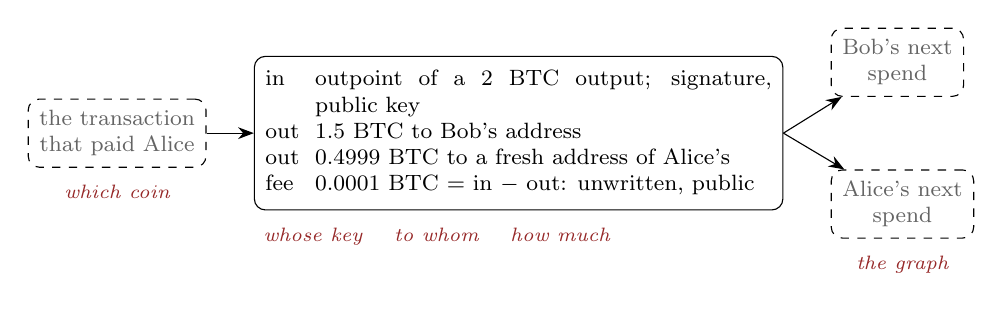
\begin{tikzpicture}[>={Stealth[length=2mm]}, font=\footnotesize,
  box/.style={draw, rounded corners, inner sep=4pt, align=left},
  ext/.style={draw, dashed, rounded corners, inner sep=4pt, align=center,
    text=arbdim},
  tag/.style={font=\scriptsize\itshape, text=arbred, align=center}]
\node[box] (tx) {\hyphenpenalty=10000 \begin{tabular}{@{}l@{\ \ }p{58mm}@{}}
  in  & outpoint of a $2$ BTC output; signature, public key \\
  out & $1.5$ BTC to Bob's address \\
  out & $0.4999$ BTC to a fresh address of Alice's \\
  fee & $0.0001$ BTC $=$ in $-$ out: unwritten, public \\
\end{tabular}};
\node[ext, left=6mm of tx] (prev) {the transaction\\ that paid Alice};
\node[ext, right=6mm of tx.east, yshift=9mm] (bobnext) {Bob's next\\ spend};
\node[ext, right=6mm of tx.east, yshift=-9mm] (alnext) {Alice's next\\ spend};
\draw[->] (prev) -- (tx);
\draw[->] (tx.east) -- (bobnext);
\draw[->] (tx.east) -- (alnext);
\node[tag, below=1mm of prev] {which coin};
\node[tag, below=1mm of alnext] {the graph};
\node[tag, below=1mm of tx.south west, anchor=north west]
  {whose key \quad to whom \quad how much};
\end{tikzpicture}}
\end{center}
\Write
The four rows of the box, in order:
\begin{itemize}
  \item \texttt{in}: outpoint of a $2$ BTC output; signature, public key
  \item \texttt{out}: $1.5$ BTC to Bob's address
  \item \texttt{out}: $0.4999$ BTC to a fresh address of Alice's
  \item \texttt{fee}: $0.0001$ BTC $=$ in $-$ out: unwritten, public
\end{itemize}
\Say
\textbf{Start where the room already is.} Alice holds one $2$ BTC output
and pays Bob $1.5$; the change goes to a fresh address of hers. Walk the
box row by row: the input names an old output by its outpoint and carries
a signature and a public key; each output carries its amount and its
spending condition.

\textbf{The names cost outside information; the graph costs nothing.}
Nobody wrote ``Alice'' or ``Bob'' on the chain, but which coin, whose
key, to whom, how much, and the arrows to the previous and the next spend
are all in the record. The fee is not even written, and it is public.

\textbf{Address reuse and change detection are structural.} Reuse an
address and its history merges. Pay with change and the non-round output
to a fresh address is usually yours. Neither is the fault of a careless
wallet; both follow from what the record has to contain.

\textbf{Keep this shape on the board.} One $2$-coin input, $1.5$ to Bob,
change back: the shielded running example has exactly this shape, with
none of the labels.
\src{\emph{Ironwood Guide}, ``The four requirements on a shielded payment''}
\end{board}

\begin{board}{The validator's four checks}{all four}
\Draw
A pseudocode block in three columns: the code on the left, the check's
number and name in the middle, what the check reads on the right. Six
lines, indented as code; the middle and right columns are filled on the
four checked lines only. Number the checks as you write them.
\Write
\begin{enumerate}
  \item \texttt{validate(tx):}
  \item \texttt{\ \ for input in tx.inputs:}
  \item \texttt{\ \ \ \ coin = utxo[input.prev\_out]}
    \quad (1) coin exists \quad reads the outpoint
  \item \texttt{\ \ \ \ check sig(input.sig, coin.script)}
    \quad (2) authorised \quad reads script and key
  \item \texttt{\ \ \ \ delete utxo[input.prev\_out]}
    \quad (3) not spent twice \quad reads the outpoint
  \item \texttt{\ \ check sum(in) >= sum(out)}
    \quad (4) conserved \quad reads every amount
\end{enumerate}
Under the block: fee $= \Sigma\,\mathrm{in} - \Sigma\,\mathrm{out}$.
\Say
\textbf{In Bitcoin the whole state is one table, the set of unspent
outputs.} A spend is a lookup, a signature check and a deletion. Write the
four checked lines and number them; these four numbers are the spine of
the workshop, and every later board names the check it serves.

\textbf{Every check reads a plaintext field} of the transaction or of the
output it names. Nothing is inferred; everything is looked at. Say what
each line reads as you write it: the outpoint, the script and the key,
the outpoint again, every amount.

\textbf{The fee is the fourth check's slack.} Sum of inputs minus sum of
outputs: not a field, yet public to the satoshi.
\src{\emph{Ironwood Guide}, ``The four requirements on a shielded payment'';
  ``Resting: the note in the commitment tree''}
\end{board}

\begin{board}{Hide a field, lose a check}{all four}
\Draw
Keep the pseudocode of the previous board (or rewrite its four checked
lines with their numbers). Then, one step at a time, in red:
\begin{enumerate}
  \item Circle \texttt{check sum(in) >= sum(out)}; write the first
    line of Write beside it.
  \item Circle \texttt{coin = utxo[input.prev\_out]} and
    \texttt{delete utxo[input.prev\_out]} together; write the second line.
  \item Circle \texttt{check sig(input.sig, coin.script)}; write the
    third line.
  \item Write ``Bob's spend, check 2'' below the block; draw an arrow to
    it from the word \texttt{script} in line 4; write the fourth line.
  \item Box the definition at the bottom of the board.
\end{enumerate}
\Write
\begin{itemize}
  \item hide the amount $\to$ check 4 dies: nothing to add up
  \item hide the input reference $\to$ checks 1 and 3 die: nothing to look
    up, nothing to delete
  \item hide the key $\to$ check 2 dies: nothing to verify against
  \item hide the receiver $\to$ nothing dies here: the output's script is
    what check 2 reads when Bob spends it, so that spend's check 2 dies
\end{itemize}
Boxed: \emph{Privacy, for this workshop: hide the sender, the receiver and
the amount, while a stranger still performs all four checks.}
\Say
\textbf{Take the plaintext away one field at a time and watch what the
node loses.} Hide the amount and check 4 dies: nothing to add up. Hide the
input reference and checks 1 and 3 die together: nothing to look up,
nothing to delete. Hide the key and check 2 dies: nothing to verify
against.

\textbf{Hiding the receiver kills nothing on this transaction.} The
output's script is what check 2 reads when Bob spends it, so it is that
later spend's check 2 that dies. The arrow makes the deferral visible.

\textbf{This is the definition to leave on the board.} Privacy, for this
workshop, means hiding the sender, the receiver and the amount while a
stranger still performs all four checks. Every mechanism to come answers
the same pair of questions: which of the four checks does it restore, and
why can the node no longer do it the Bitcoin way?
\src{\emph{Ironwood Guide}, ``The four requirements on a shielded payment'';
  ``What a node verifies, without ever observing the note''}
\end{board}

\begin{board}{What a privacy design must supply}{all four}
\Draw
A table, three columns: \emph{the validator must} $\mid$ \emph{the tool}
$\mid$ \emph{Bitcoin's version}. Four rows, in this order: accept a claim
about data it cannot see; know the hidden data cannot change under it;
notice the same hidden coin a second time; add up amounts it cannot read.
Fill each row across before starting the next.
\Write
\begin{enumerate}
  \item accept a claim about data it cannot see $\mid$ a zero-knowledge
    proof: the statement public, the witness (the prover's secret input,
    not Bitcoin's witness field) private $\mid$ look at the data
  \item know the hidden data cannot change under it $\mid$ a commitment:
    hiding, and binding $\mid$ the output, in the clear
  \item notice the same hidden coin a second time $\mid$ a nullifier: a
    keyed, one-way tag of the coin, published at spend $\mid$ delete it
    from the set
  \item add up amounts it cannot read $\mid$ a homomorphic commitment:
    sealed envelopes that add $\mid$ add the numbers
\end{enumerate}
Under the table: \emph{the proof checks the claim; the other three tools
make the claim about something fixed, unrepeatable, summable.}
\Say
\textbf{Each dead check names a capability the design must supply.} Read
the table row by row against Bitcoin's version. Where the Bitcoin node
looks at the data, this validator must accept a claim about data it cannot
see: a zero-knowledge proof, statement public, witness private. Say at
once that ``witness'' here is the prover's secret input, not Bitcoin's
witness field.

\textbf{The proof alone is not enough: the claim must be about something
fixed.} Where Bitcoin has the output in the clear, a commitment, hiding
and binding, pins the hidden data so it cannot change under the
validator.

\textbf{Where Bitcoin deletes the coin from the set, a nullifier lets the
validator notice the same hidden coin a second time:} a keyed, one-way tag
of the coin, published at spend.

\textbf{Where Bitcoin adds the numbers, a homomorphic commitment adds
sealed envelopes.} The next board shows the one line that makes it work.

\textbf{Emphasise the division of labour.} The proof checks the claim; the
other three tools make the claim about something fixed, unrepeatable,
summable.
\Avoid
``The proof hides the sender and the receiver.'' On this board the proof
only checks a claim about hidden data; what hides is the commitment's
hiding property and the keyed tag (key re-randomisation joins them on
``Four checks, four mechanisms''). Keep the proof in its column.
\src{\emph{Crypto Guide}, ``Three questions''; ``The sealed envelope'';
  \emph{Ironwood Guide}, ``The nullifier, and the loop back to minting''}
\end{board}

\begin{board}{Sealed envelopes that add}{conserved}
\Write
\[
\bigl([v_1]\,V + [r_1]\,R\bigr) + \bigl([v_2]\,V + [r_2]\,R\bigr)
  = [v_1 + v_2]\,V + [r_1 + r_2]\,R
\]
Beside it: \emph{holds modulo the group order; the $64$-bit range check
lives inside the proof.}
\Say
\textbf{The fourth tool in one line: two commitments add without either
being opened.} Write the sum and point at the right-hand side: the two
sealed envelopes combine into an envelope for the sum of the values, with
the sum of the randomness.

\textbf{The room knows this trick.} It is the Confidential Transactions
trick: amounts hidden, their sum still checkable.

\textbf{Emphasise the gap and where it is closed.} The identity holds only
modulo the group order; here the $64$-bit range check that closes the gap
lives inside the proof.
\src{\emph{Crypto Guide}, ``The Pedersen commitment''; \emph{Ironwood
  Guide}, ``Conservation without disclosure: value commitments and the
  binding signature''; ``The Action statement, formally''}
\end{board}

\begin{board}{Notes versus UTXOs: what a coin is}{authorised, conserved}
\Draw
A table, three columns: (blank) $\mid$ \emph{Bitcoin UTXO} $\mid$
\emph{Zcash note}. Three rows, in this order: owner; value; spending
condition. Fill each row across.
\Write
\begin{enumerate}
  \item owner $\mid$ a script, usually one key hash, on chain $\mid$ an
    address $(d, \pkd)$, inside the note
  \item value $\mid$ the amount, on chain $\mid$ $v \in [0, 2^{64})$
    zatoshi, inside the note
  \item spending condition $\mid$ script: signatures, timelocks, hashlocks
    $\mid$ a key, full stop --- no script, no timelocks, no HTLCs
\end{enumerate}
\Say
\textbf{What a coin is, side by side.} In Bitcoin the owner is a script,
usually one key hash, written on the output, and the value is written
beside it. In Zcash both are fields of the note, an address $(d, \pkd)$
and a value $v$ in $[0, 2^{64})$ zatoshi, and the note is never
published.

\textbf{The spending condition is a key, full stop.} No script, no
timelocks, no HTLCs.

\textbf{Threshold authority exists and is invisible on chain.} It is
FROST, later in the workshop; on chain there is one ordinary signature
under one per-spend key.
\src{\emph{Ironwood Guide}, ``The note and its commitment''; ``Spend
  authorisation: RedPallas re-randomisation''; \emph{FROST Guide}, ``The
  three deployment surfaces''}
\end{board}

\begin{board}{Notes versus UTXOs: what the chain records}{exists, not twice}
\Draw
A table, three columns: (blank) $\mid$ \emph{Bitcoin UTXO} $\mid$
\emph{Zcash note}. Three rows, in this order: on-chain identifier; spent
marker; set structure. Fill each row across.
\Write
\begin{enumerate}
  \item on-chain identifier $\mid$ the outpoint $\mid$ a commitment
    $\cmsym$ to the note, stored as $\cmx$
  \item spent marker $\mid$ removed from the UTXO set $\mid$ a nullifier
    $\nfsym$, published at spend
  \item set structure $\mid$ one set: insert, delete $\mid$ an append-only
    tree of $\cmx$, depth $32$, and a set of $\nfsym$: append only, both
\end{enumerate}
Under the table: \emph{the note never touches the chain.}
\Say
\textbf{What the chain records, side by side.} Bitcoin identifies a coin by
its outpoint; Zcash by a commitment $\cmsym$ to the note, stored as
$\cmx$. Bitcoin marks a coin spent by removing it from the UTXO set; Zcash
by publishing a nullifier $\nfsym$ at spend.

\textbf{The set structures differ in kind.} Bitcoin keeps one set
with insert and delete. Zcash keeps two append-only structures: a tree of
$\cmx$ of depth $32$ and a set of $\nfsym$. Nothing is ever deleted.

\textbf{Emphasise: the note never touches the chain.} Recorded are a
commitment to it, an encrypted copy for its recipient, and at spend a tag
derived from it.
\src{\emph{Ironwood Guide}, ``The note and its commitment''; ``The tree, its
  hash, and its anchors''; ``The nullifier, and the loop back to minting''}
\end{board}

\begin{board}{The three-line mental model}{all four}
\Write
A shielded spend is three claims about a note nobody sees:
\begin{enumerate}
  \item \emph{it exists} --- a commitment to it is a leaf under a public
    root, proved with leaf, position and path all private;
  \item \emph{it is spent now} --- its serial number, the nullifier, is
    revealed, and the chain refuses to see it twice;
  \item \emph{the books balance} --- commitments to the amounts add up to
    the declared net flow.
\end{enumerate}
Under line 1:
\[
R_{\mathrm{mem}} = \bigl\{\, (\underbrace{\mathit{rt}}_{\text{public}};\
  \underbrace{(\cmx,\ i,\ \mathit{path})}_{\text{private}}) \ :\
  \mathsf{Verify}(\mathit{rt}, i, \cmx, \mathit{path}) = \mathsf{accept}
  \,\bigr\}
\]
\Say
\textbf{A shielded spend is three claims about a note nobody sees.} Write
them as three numbered lines. It exists: a commitment to it is a leaf
under a public root, proved with leaf, position and path all private. It
is spent now: its serial number, the nullifier, is revealed, and the chain
refuses to see it twice. The books balance: commitments to the amounts add
up to the declared net flow.

\textbf{Write the membership relation under line 1.} The root is the
public part; the commitment, its index and the path are the private
witness; the relation holds when the path verifies.

\textbf{A Bitcoin spend names its coin and signs; a shielded spend names
nothing.} It proves the first line, reveals the second and signs for the
third. And, as in Bitcoin, the spender signs, under a key the proof ties
to the note: that is check 2.

\textbf{Emphasise:} everything else in the workshop is machinery for these
three lines and for that signature.
\Avoid
Letting the position $i$ migrate into line 2. The index is a private
witness of line 1 only; the nullifier is a tag derived from the note (the
previous board), not from where the note sits in the tree.
\src{\emph{Crypto Guide}, ``Privacy-preserving membership via zero-knowledge
  paths''; ``A shielded spend, end to end''; \emph{Ironwood Guide},
  ``Conservation without disclosure: value commitments and the binding
  signature''}
\end{board}

\begin{board}{Four checks, four mechanisms}{all four}
\Draw
A table, four columns: (number) $\mid$ \emph{the check} $\mid$
\emph{Bitcoin} $\mid$ \emph{shielded Zcash}. Four rows in the order (1),
(3), (4), (2), the order the workshop takes them. Fill each row across.
\Write
\begin{enumerate}
  \item (1) coin exists $\mid$ look the outpoint up in the UTXO set $\mid$
    a commitment in an append-only tree; a membership proof under a
    public root
  \item (3) not spent twice $\mid$ delete it from the set $\mid$ a
    nullifier, published once, refused the second time
  \item (4) conserved $\mid$ add the amounts up $\mid$ value commitments
    that add; a binding signature over their sum
  \item (2) authorised $\mid$ run the script over the signature $\mid$ key
    knowledge proved inside the proof; a signature under a re-randomised
    key
\end{enumerate}
\Say
\textbf{Each right-hand cell names what replaces one Bitcoin check.} Coin
exists: a commitment in an append-only tree and a membership proof under
a public root. Not spent twice: a nullifier, published once, refused the
second time. Conserved: value commitments that add and a binding
signature over their sum. Authorised: key knowledge proved inside the
proof and a signature under a re-randomised key.

\textbf{Why the Bitcoin way is gone was settled on the board ``Hide a
field, lose a check''.} Point back at it. Each part of the workshop
reopens with both questions: which check, and why not the Bitcoin way.

\textbf{Emphasise the order.} Checks 1 and 3 come first, with the data
model; checks 4 and 2 follow, on the running example.
\Avoid
Glossing the re-randomised key as a multiple of $\aksym$. The disguise is
additive; its formula comes later, and this table only names it.
\src{\emph{Ironwood Guide}, ``The four requirements on a shielded payment'';
  ``The Action statement, formally''}
\end{board}

\begin{board}{The route}{all four}
\Write
The ten parts, as a numbered list:
\begin{enumerate}
  \item \textbf{The toolbox} --- each primitive from the Bitcoin instance
    the room already holds.
  \item \textbf{The data model} --- notes, commitments, the tree, the
    nullifier: checks 1 and 3.
  \item \textbf{Keys and addresses} --- who can spend, who can see.
  \item \textbf{The Action statement} --- what the proof proves, clause by
    clause; then a break.
  \item \textbf{Balance and authority} --- checks 4 and 2, on the running
    example.
  \item \textbf{The proof system} --- from a statement to a few kilobytes.
  \item \textbf{Delivery and light clients} --- how Bob finds his money.
  \item \textbf{The transaction and the turnstile} --- the bytes on the
    chain, and the pools.
  \item \textbf{Consensus} --- why one fork wins, what the chain must
    remember.
  \item \textbf{Limits, frontier, takeaways.}
\end{enumerate}
Under the list: \emph{one example threads it: Alice pays Bob $1.5$ ZEC
from a $2$ ZEC note.}
\Say
\textbf{The route follows the checks.} The toolbox first, each primitive
from the Bitcoin instance the room already holds; the data model for
checks 1 and 3; keys and addresses; the Action statement clause by
clause, then the break; balance and authority for checks 4 and 2; the
proof system; delivery; the transaction and the turnstile; consensus;
limits and frontier.

\textbf{One example threads it.} Alice pays Bob $1.5$ ZEC from a $2$ ZEC
note: the Bitcoin shape of the first board, without its labels.

\textbf{Close Part A with the checkpoint.} Put the question on the board
and take answers before giving yours.
\Ask
\emph{Which of the four checks does a nullifier serve, and what breaks if
two different notes could share one?}
\begin{itemize}
  \item Check 3, not spent twice. The nullifier is ``delete from the UTXO
    set'' without naming the coin: published once, refused the second
    time.
  \item Two notes, one nullifier: whichever is spent first burns the other,
    and the second owner's honest spend is refused as a double spend ---
    an attack on earlier designs, in which forged notes could be made to
    share one.
  \item How the chain makes sure no two accepted notes can share one ---
    every new note inherits, as its seed, the serial of the note spent
    beside it --- is Part C's business.
\end{itemize}
\Avoid
``A few hundred bytes'' for the proof: the route says a few kilobytes, and
the proof-system part gives the number. The seed a new note inherits is
the serial of the note spent beside it, not a position in the tree.
\src{\emph{Ironwood Guide}, ``The nullifier, and the loop back to minting''}
\end{board}

%% ---- 02-toolbox.tex
%% Part B --- The toolbox, from Bitcoin's primitives up. Whiteboard notes,
%% drafted from draft/02-toolbox.tex. Every number is the deck's
%% (compute/b_primitives.py, b_proofsizes.py, g_twoadic.py, e_tree.py).

\section{Part B --- The toolbox, from Bitcoin's primitives up}

One board per primitive, or per property of one: what it is in a line,
the Bitcoin instance the room already holds, the Zcash instance, the
property the protocol spends, and where it returns. The check in each
header is the spine; ``all four'' marks a primitive every check rests on.

%% ---------------------------------------------------------------- B1
\begin{board}{Hash functions: one primitive, three notions}{all four}
\Write
\begin{enumerate}
  \item $H \colon \{0,1\}^{*} \to \{0,1\}^{n}$ --- fixed, public,
    compresses
  \item preimage: given $y$, find $x'$ with $H(x') = y$
  \item second preimage: given $x$, find $x' \ne x$ with $H(x') = H(x)$
  \item collision: find any $x \ne x'$ with $H(x) = H(x')$ --- strongest;
    commitments, Merkle trees, Fiat--Shamir
  \item generic: collision $\approx 2^{n/2}$ (birthday), preimage
    $\approx 2^{n}$; $n = 256 \Rightarrow 2^{128}$; RIPEMD-160
    $\Rightarrow 2^{80}$
  \item Bitcoin: SHA-256d (headers, txids);
    $\mathsf{hash160} = \mathrm{RIPEMD160} \circ \mathrm{SHA256}$
    (addresses)
  \item Zcash: keeps all of these (transparent) $+$ three shielded hashes
\end{enumerate}
\Say
\textbf{Start from the primitive the room already trusts.} A hash is a
fixed public function from arbitrary strings to $n$ bits. Write the three
notions in order of strength: preimage, second preimage, collision. In the
collision game the adversary picks both inputs, so it is the strongest
demand --- and the one commitments, Merkle trees and Fiat--Shamir need.

\textbf{The generic costs set the digest sizes.} A collision after about
$2^{n/2}$ evaluations, the birthday bound; a preimage after $2^{n}$. That
is why a $256$-bit digest buys $128$-bit collision security, and why
RIPEMD-160 sits at $2^{80}$.

\textbf{Bitcoin contrast: nothing is taken away.} SHA-256d over every
block header and every txid; $\mathsf{hash160}$ inside addresses. Zcash
keeps every one of those in its transparent layer and adds three hashes
for the shielded one --- next board.
\Ask
Which of the three notions do commitments and Merkle trees lean on?
Collision resistance: the adversary picks both inputs.
\src{\emph{Crypto Guide}, ``Security notions: preimage, second-preimage,
  and collision resistance''; ``The birthday bound on generic collision
  finding''; ``The transparent layer's hashes''}
\end{board}

\begin{board}{Zcash's hashes: SHA-256 is not replaced}{all four}
\Draw
Three columns --- \emph{hash}, \emph{kind}, \emph{deployed use} --- then
four rows, in this order:
\begin{enumerate}
  \item SHA-256d --- bit-oriented, Bitcoin's --- header difficulty filter
    (after Equihash); transparent layer: legacy txids, Base58Check.
  \item BLAKE2b --- bit-oriented; personalised natively, the key prepended
    to the input --- $\mathsf{PRFexpand}$ (the key tree); note-encryption
    KDF; ZIP-244 digests (txid, sighash).
  \item Poseidon --- algebraic: $x \mapsto x^{5}$ over $\Fpp$ --- the
    nullifier PRF, inside the circuit.
  \item Sinsemilla --- algebraic: curve additions on \Pallas{} --- note
    commitment; Merkle node hash, both inside the circuit.
\end{enumerate}
\Write
\begin{enumerate}
  \item Bitcoin's hashes stay where Bitcoin put them
  \item shielded: $+1$ bit-oriented (off the circuit), $+2$ algebraic
    (inside it)
\end{enumerate}
\Say
\textbf{The first row answers the question the room is about to ask.}
SHA-256d is still there: the header difficulty filter after Equihash,
and the transparent layer's legacy txids and Base58Check.

\textbf{Three hashes are added, and the split is by where the work
happens.} BLAKE2b, bit-oriented and personalised natively with the key
prepended, does the work off the circuit: $\mathsf{PRFexpand}$ for the
key tree, the note-encryption KDF, the ZIP-244 txid and sighash digests.
Poseidon, an algebraic hash built on $x \mapsto x^{5}$ over $\Fpp$, is the
nullifier PRF inside the circuit. Sinsemilla, curve additions on \Pallas{},
is the note commitment and the Merkle node hash, both inside the circuit.

\textbf{Emphasise the closing line.} Bitcoin's hashes stay where Bitcoin
put them; the shielded protocol adds one bit-oriented hash for work off
the circuit and two algebraic ones for work inside it. Poseidon and
Sinsemilla return in Part C; BLAKE2b in Parts D, F and H.
\Avoid
``SHA-256 is replaced by BLAKE2b'' --- it is not replaced; it keeps the
header filter and the transparent layer.
\src{\emph{Consensus Guide}, ``Equihash and the memoryless model'';
  \emph{Crypto Guide}, ``The transparent layer's hashes''; ``PRFs from hash
  functions: length extension and keyed BLAKE2''; ``Arithmetisation-friendly
  hashing: Poseidon''; \emph{Ironwood Guide}, ``Sinsemilla: hash,
  commitment, and short forms''}
\end{board}

\begin{board}{Why in-circuit hashing wants algebraic hashes}{exists,
  not twice}
\Write
\begin{enumerate}
  \item proof $=$ polynomial constraints over a prime field; field
    multiplication $=$ 1 constraint; Boolean operation $=$ several $+$
    range checks
  \item SHA-256, BLAKE2: 32-/64-bit words, XOR, shuffles $\Rightarrow$ tens
    of thousands of constraints per evaluation
  \item Poseidon round: $+$ constants; $x^{5}$ (all elements in a full
    round, one in a partial); $\times$ fixed matrix. 2-to-1 hash $\approx$
    a few hundred constraints. Orchard: width 3, 8 full $+$ 56 partial
  \item Sinsemilla, per 10-bit chunk: 1 lookup (table of $2^{10} = 1024$
    points) $+$ 2 incomplete additions; collision $\Rightarrow$ discrete
    log
\end{enumerate}
\Say
\textbf{Why the shielded layer needs hashes of a different kind.} A
zero-knowledge proof re-expresses every step of a computation as
polynomial constraints over a prime field. A field multiplication is one
constraint; a Boolean operation is several, plus range checks.

\textbf{SHA-256 and BLAKE2 are foreign to the field.} They shuffle and
XOR $32$- and $64$-bit words: tens of thousands of constraints per
evaluation.

\textbf{Poseidon keeps the only non-linear step at $x^{5}$.} Add
constants, raise the state to the fifth power --- every element in a full
round, one element in a partial round --- multiply by a fixed matrix. A
$2$-to-$1$ hash costs a few hundred constraints. Orchard's instance: state
width $3$, $8$ full and $56$ partial rounds.

\textbf{Sinsemilla is curve arithmetic, native to the circuit.} Per
$10$-bit chunk, one lookup into a table of $2^{10} = 1024$ hashed-to-curve
points and two incomplete curve additions; its collision resistance
reduces to the discrete logarithm.

\textbf{Bitcoin contrast:} Bitcoin never hashes inside a proof. The first
shielded generation did, with SHA-256, and its prover paid for it.
\Avoid
Timing claims: ``its prover paid for it'' stays qualitative; no seconds or
minutes for the first generation's prover.
\src{\emph{Crypto Guide}, ``Arithmetisation-friendly hashing: Poseidon'';
  ``Sinsemilla: an algebraic hash-based commitment''; \emph{Ironwood Guide},
  ``Why Sinsemilla: in-circuit cost''; ``Lineage: three generations of
  shielded proof''}
\end{board}

%% ---------------------------------------------------------------- B2
\begin{board}{Curves: the same shape, different primes}{all four}
\Write
\begin{enumerate}
  \item $y^{2} = x^{3} + b$ over a prime field; prime-order group, cofactor
    $1$; discrete log $=$ the standing assumption
  \item secp256k1: $b = 7$, $p = 2^{256} - 2^{32} - 977$, $256$-bit prime
    order
  \item \Pallas{}, \Vesta{}: $b = 5$, two $255$-bit primes $p_{\Pallas}$,
    $p_{\Vesta}$; $\#\Pallas = p_{\Vesta}$, $\#\Vesta = p_{\Pallas}$;
    $\approx 126$ bits of DL security
  \item generators: hashed to the curve (secp256k1's base point: a SEC~2
    constant)
  \item \Pallas{}: every point in an Action; \Vesta{}: the proof's
    polynomial commitments
\end{enumerate}
\Say
\textbf{The same shape the room knows.} Short Weierstrass $y^{2} = x^{3}
+ b$ over a prime field; the points form a group of prime order, cofactor
$1$; the discrete logarithm in it is the standing assumption.

\textbf{Bitcoin:} secp256k1, $b = 7$ over $p = 2^{256} - 2^{32} - 977$,
a $256$-bit prime order. The room's keys, ECDSA and BIP-340 live here.

\textbf{Zcash:} \Pallas{} and \Vesta{}, $b = 5$ over two $255$-bit
primes, with the twist on the board: $\#\Pallas = p_{\Vesta}$ and
$\#\Vesta = p_{\Pallas}$ --- the scalar field of each is the base field
of the other. About $126$ bits of discrete-log security.

\textbf{Every generator is hashed to the curve.} The secp256k1 base point
is a SEC~2 constant; every \Pallas{} and \Vesta{} generator the protocol
uses is hashed, so no relation between any two is known to anyone, and
there is no ceremony for this stack. Say the caveat in the same breath:
the Sapling pool still rests on its Groth16 MPC (Part G).

\textbf{Division of labour, explained in Part G:} \Pallas{} carries every
point in an Action --- commitments, nullifier base, keys, ephemeral keys,
signatures; \Vesta{} carries the proof's polynomial commitments.
\Avoid
``No ceremony'' without the Sapling caveat: no ceremony for this stack;
the Sapling pool still rests on its Groth16 MPC.
\src{\emph{Crypto Guide}, ``Instantiation on elliptic curves; the Pasta
  curves''; ``The transparent layer's schemes: ECDSA and BIP-340 over
  secp256k1''; \emph{Math Guide}, ``Pallas and Vesta assembled''}
\end{board}

\begin{board}{Why not secp256k1: two-adicity}{all four}
\Draw
Four columns --- \emph{field}, \emph{bits}, \emph{two-adicity of $p - 1$},
\emph{largest power-of-two domain} --- then four rows, in this order:
\begin{enumerate}
  \item \Pallas{} base field --- $255$ --- $32$ --- $2^{32}$.
  \item \Vesta{} base field --- $255$ --- $32$ --- $2^{32}$.
  \item secp256k1 base field --- $256$ --- $1$ --- $2$.
  \item secp256k1 scalar field --- $256$ --- $6$ --- $64$.
\end{enumerate}
\Write
\begin{enumerate}
  \item $2^{k}$-th roots of unity exist iff $2^{k} \mid p - 1$; largest
    such $k$ $=$ two-adicity
  \item Orchard circuit: $2^{11}$ rows
  \item secp256k1 rows: our own computation, not a volume figure
\end{enumerate}
\Say
\textbf{Why not simply use secp256k1?} A proof system of the PLONK family
interpolates each circuit column over the $2^{k}$-th roots of unity of
its field. Those exist iff $2^{k} \mid p - 1$; the largest such $k$ is
the field's two-adicity.

\textbf{Read the table.} The \Pallas{} and \Vesta{} base fields: $255$
bits, two-adicity $32$, a domain of $2^{32}$. The secp256k1 base field:
two-adicity $1$, a domain of size $2$; its scalar field: $6$, a domain of
$64$.

\textbf{The Orchard circuit has $2^{11}$ rows.} Neither secp256k1 field
offers a domain of that size. The Pasta primes were searched for with
two-adicity $32$ and the cycle as design goals.

\textbf{Label the provenance.} The secp256k1 rows are the deck's own
computation, not a volume figure; say so. Rows, roots of
unity and the polynomial identity return in Part G.
\Ask
Which secp256k1 field could host $2^{11}$ rows? Neither: the largest
domains are $2$ and $64$.
\src{\emph{Math Guide}, ``Roots of unity and evaluation domains'', Remark
  ``Two-adicity and FFT-friendly primes''; ``Base fields, scalar fields, and
  the Pasta cycle''; \emph{Crypto Guide}, ``The transparent layer's schemes:
  ECDSA and BIP-340 over secp256k1''}
\end{board}

%% ---------------------------------------------------------------- B3
\begin{board}{Commitments: a sealed envelope}{exists, conserved}
\Write
\begin{enumerate}
  \item $c = \Comm(m; r)$, trapdoor $r$; hiding: two candidate $m$
    indistinguishable from $c$; binding: no $c$ opens to two $m$
  \item not both perfect; deployed: perfectly hiding, binding under DL
  \item $\Comm(v; r) := [v]\,V + [r]\,R$, with $V, R$ hashed to \Pallas{}
  \item uniform $r \Rightarrow$ uniform point; two openings $\Rightarrow
    \log_{V} R$
  \item Bitcoin: CT's envelope; an address $=$ hash commitment to a
    key/script, opened at spend
  \item Zcash: $\cvsym$ seals the value change (Pedersen, adds); $\cmsym$
    seals the whole note (algebraic hash $+ [\rcm]\,H_{D}$)
\end{enumerate}
\Say
\textbf{A commitment is a sealed envelope.} Commitment $c = \Comm(m; r)$
with a random trapdoor $r$. Hiding: from $c$, two candidate messages are
indistinguishable. Binding: no $c$ opens to two messages. The two cannot
both be perfect; the deployed schemes are perfectly hiding and binding
under the discrete logarithm.

\textbf{Pedersen on \Pallas{}, with $V$ and $R$ hashed to the curve.}
Write $\Comm(v; r) := [v]\,V + [r]\,R$. For uniform $r$ the point is
uniform whatever $v$ is --- that is hiding. Two openings of one $c$ solve
$\log_{V} R$, which nobody holds --- that is binding.

\textbf{Bitcoin contrast.} This envelope is Confidential Transactions';
and an address is already a hash commitment to a public key or a script,
opened at spend.

\textbf{Zcash has two envelopes per Action.} The value commitment
$\cvsym$ seals an Action's value change --- Pedersen, so it adds. The note
commitment $\cmsym$ seals a whole note: an algebraic hash plus a blinding
term $[\rcm]\,H_{D}$ of the same Pedersen shape, over its own hashed
generator, so the circuit recomputes it cheaply.
\Ask
Can the envelope be perfectly hiding and perfectly binding at once? No;
the deployed ones are perfectly hiding and binding under the discrete
logarithm.
\src{\emph{Crypto Guide}, ``Hiding and binding''; ``The Pedersen
  commitment''; ``Sinsemilla: an algebraic hash-based commitment'';
  \emph{Ironwood Guide}, ``Sinsemilla: hash, commitment, and short forms''}
\end{board}

\begin{board}{The envelope adds: the Confidential Transactions
  bridge}{conserved}
\Write
\begin{enumerate}
  \item $\Comm(v_{1}; r_{1}) + \Comm(v_{2}; r_{2})
    = \Comm(v_{1} + v_{2};\ r_{1} + r_{2})$
  \item \[
      \sum \Comm_{\mathrm{in}} - \sum \Comm_{\mathrm{out}}
      = \Bigl[\sum v_{\mathrm{in}} - \sum v_{\mathrm{out}}\Bigr] V
        + [\bar r]\,R
    \]
  \item $V$ term vanishes iff values balance --- modulo the group order;
    range check on every value closes the wrap
  \item CT (Elements): same equation on chain; range proof beside each
    commitment; receiver told the opening; amounts hidden, keys and graph
    clear
  \item here: $64$-bit range check $+$ opening $(v, \rcv)$ $=$ clauses of
    one ZK proof; net trapdoor $\bar r \to$ a signing key
\end{enumerate}
\Say
\textbf{The envelope adds.} Two commitments sum to a commitment to the
summed values under the summed trapdoors. Sum the inputs, subtract the
outputs: the $V$ term carries $\sum v_{\mathrm{in}} - \sum
v_{\mathrm{out}}$ and vanishes exactly when the values balance --- modulo
the group order. A range check on every value closes the wrap.

\textbf{Bitcoin contrast: Confidential Transactions (Elements).} The same
equation on the chain; a range proof beside each commitment; the receiver
is told the opening. Amounts hidden, keys and graph in the clear.

\textbf{Here the equation moves inside the proof.} The $64$-bit range
check and the opening $(v, \rcv)$ are clauses of one zero-knowledge proof,
alongside the sender's authorisation and the receiver's note; the net
trapdoor $\bar r$ becomes a signing key --- the board \emph{Preview: a
signature under a key nobody holds unless the values balance} shows how.
Clause A4 in Part E; the balance walk-through in Part E$'$.
\src{\emph{Crypto Guide}, ``The Pedersen commitment''; ``Binding signatures
  as a proof of knowledge of a discrete logarithm''}
\end{board}

%% ---------------------------------------------------------------- B4
\begin{board}{Merkle trees: from the txid tree to the note commitment
  tree}{exists}
\Draw
\begin{enumerate}
  \item At the top, a rounded box labelled \emph{anchor}.
  \item Under it two circles; under each, two more; under each of those,
    two small boxes --- eight leaves. Label the leaves $\cmx$ left to
    right; draw the eighth dashed and label it $\varnothing$, the empty
    slot.
  \item In red: the third leaf, its parent circle and its grandparent (the
    left level-one circle) --- the spent note and its route to the root.
  \item In green: the sibling at each level of that route --- the fourth
    leaf, the first level-two circle, the right level-one circle.
  \item Legend under the tree: red $=$ the leaf and its route, private;
    green $=$ the siblings, private; the anchor alone is public.
\end{enumerate}
\begin{center}
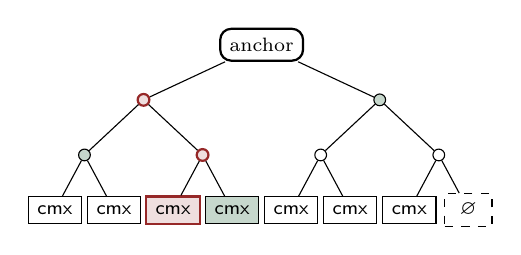
\begin{tikzpicture}[every node/.style={font=\scriptsize},level distance=7mm,
  level 1/.style={sibling distance=30mm},
  level 2/.style={sibling distance=15mm},
  level 3/.style={sibling distance=7.5mm},
  nd/.style={draw,circle,inner sep=1.5pt},
  lf/.style={draw,minimum width=6mm},
  rt/.style={draw=arbred,thick,fill=arbred!15},
  sb/.style={fill=arb!25}]
\node[draw,rounded corners,thick] {anchor}
  child {node[nd,rt] {}
    child {node[nd,sb] {}
      child {node[lf] {\cmx}}
      child {node[lf] {\cmx}}}
    child {node[nd,rt] {}
      child {node[lf,rt] {\cmx}}
      child {node[lf,sb] {\cmx}}}}
  child {node[nd,sb] {}
    child {node[nd] {}
      child {node[lf] {\cmx}}
      child {node[lf] {\cmx}}}
    child {node[nd] {}
      child {node[lf] {\cmx}}
      child {node[lf,dashed] {$\varnothing$}}}};
\end{tikzpicture}
\par
{\scriptsize red: the leaf and its route, private; green: the siblings,
private; the anchor alone is public}
\end{center}
\Write
\begin{enumerate}
  \item Bitcoin: txids pairwise up to the header root; SPV proof $=$ leaf
    $+$ one sibling per level; the leaf (txid) is public
  \item Zcash: leaves $= \cmx$ in creation order; depth $32$, room for
    $2^{32}$ notes; node hash Sinsemilla, tagged with its layer; root after
    each block $=$ that block's \emph{anchor}
  \item membership proof: $32$ siblings $+$ $32$ direction bits, verified
    by $32$ hashes --- inside the proof
\end{enumerate}
\Say
\textbf{Bitcoin's tree the room knows.} Each block hashes its txids
pairwise up to a root in the header; an SPV proof is the leaf plus one
sibling per level --- and the leaf, the txid, is public.

\textbf{Zcash's tree.} The leaves are $\cmx$ in creation order; depth
$32$, room for $2^{32}$ notes; the node hash is Sinsemilla, tagged with
its layer; the root after each block is that block's anchor.

\textbf{A membership proof is $32$ siblings and $32$ direction bits,
verified by $32$ hashes} --- recomputed here inside the proof. Point at
the tree: red is the leaf and its route, private; green the siblings,
private; the anchor alone is public.
\src{\emph{Crypto Guide}, ``Authentication paths and membership proofs'';
  \emph{Ironwood Guide}, ``The tree, its hash, and its anchors''}
\end{board}

\begin{board}{What changes: append only, historical roots, private
  path}{exists}
\Write
\begin{enumerate}
  \item append only: one leaf at a time; frontier $\le 32$ carried labels;
    root updated in $32$ hashes; nothing deleted --- ``deleted'' $=$ a
    separate set
  \item history binding: proof against the root at insertion valid
    forever; consensus accepts the anchor of any earlier main-chain block
  \item private path: (leaf, index, siblings) $=$ witness; anchor $=$
    statement
  \item \[
      R_{\mathrm{mem}} = \bigl\{\,(\mathit{rt};\ (\cmx, i, \mathit{path})) :
        \mathsf{Verify}(\mathit{rt}, i, \cmx, \mathit{path})
        = \mathsf{accept}\,\bigr\}
    \]
  \item Bitcoin SPV names the txid; this proof names only the root
\end{enumerate}
\Say
\textbf{Append only.} One leaf at a time; the frontier --- at most $32$
carried labels --- updates the root in $32$ hashes. Nothing is ever
deleted; the ``deleted'' half of the state is a separate set.

\textbf{History binding.} A proof formed against the root at insertion
stays valid against that root forever, and consensus accepts the anchor
of any earlier main-chain block.

\textbf{Private path.} Revealing (leaf, index, siblings) would say which
note is spent; so the path is a witness of the zero-knowledge proof and
only the anchor is a statement. Write the relation: the statement is the
root $\mathit{rt}$, the witness is $(\cmx, i, \mathit{path})$.

\textbf{Bitcoin contrast:} an SPV proof names the txid it proves; this
proof names only the root and hides the leaf among every leaf beneath it.
The tree, anchors and the nullifier set in Part C; clause A3 in Part E.
\src{\emph{Crypto Guide}, ``Append-only and incrementally updatable trees'';
  ``Privacy-preserving membership via zero-knowledge paths'';
  \emph{Ironwood Guide}, ``The tree, its hash, and its anchors''}
\end{board}

%% ---------------------------------------------------------------- B5
\begin{board}{Pseudorandom functions: a key that fakes randomness}{not
  twice}
\Write
\begin{enumerate}
  \item $F_{k}$ pseudorandom: secret uniform $k$; no efficient adversary
    with oracle access (any inputs, adaptively) tells $F_{k}$ from a
    random function
  \item algorithm public; only $k$ hidden; adversary sees input--output
    pairs, never $k$
  \item Bitcoin: HMAC-SHA512 in BIP-32 child derivation
  \item Zcash, off circuit: BLAKE2b personalised $= \mathsf{PRFexpand}$;
    $\mathsf{sk} \to \asksym, \nksym, \rivk$; later the note's randomness
    from its seed
  \item Zcash, in circuit: $F_{\nksym}(\rho) = \mathsf{PoseidonHash}(\nksym,
    \rho)$ over $\Fpp$; width $3$, S-box $x^{5}$, $8$ full $+$ $56$
    partial rounds
\end{enumerate}
\Say
\textbf{A PRF is a key that fakes randomness.} A keyed function $F_{k}$
is pseudorandom if, for a secret uniform $k$, no efficient adversary with
oracle access --- any inputs, adaptively --- tells $F_{k}$ from a truly
random function. The algorithm is public; only $k$ is hidden; the
adversary sees input--output pairs of her choosing and never $k$.

\textbf{Bitcoin:} HMAC-SHA512 inside BIP-32 child derivation --- a PRF
the room already trusts to make child keys look unrelated.

\textbf{Zcash, off the circuit:} BLAKE2b, personalised, as
$\mathsf{PRFexpand}$ --- one call per sub-secret, $\mathsf{sk} \to
\asksym, \nksym, \rivk$, and later the note's randomness from its seed.
It builds the key ladder in Part D.

\textbf{Zcash, inside the circuit:} Poseidon over $\Fpp$, keyed by its
first input --- $\nksym$ first, $\rho$ second, as written on the board;
state width $3$, S-box $x^{5}$, $8$ full and $56$ partial rounds.
\src{\emph{Crypto Guide}, ``Pseudorandom functions and permutations'';
  ``PRFs from hash functions: length extension and keyed BLAKE2'';
  ``Arithmetisation-friendly hashing: Poseidon''}
\end{board}

\begin{board}{What a nullifier needs from a PRF}{not twice}
\Write
\begin{enumerate}
  \item \[
      \nfsym = \Extract\bigl([\,F_{\nksym}(\rho) + \psi\,]\,G^{\mathsf{nf}}
        + \cmsym\bigr)
    \]
  \item $\Extract$: the $x$-coordinate; $\rho, \psi$: per-note randomness
    fixed at creation; $G^{\mathsf{nf}}$: a hashed generator
  \item uniqueness: all inputs fixed once the note exists $\Rightarrow$
    deterministic; two notes, one tag $\Rightarrow$ DL relation on
    \Pallas{}; no PRF property used (forger holds $\nksym$)
  \item unlinkability: without $\nksym$, $[F_{\nksym}(\rho) + \psi]\,
    G^{\mathsf{nf}}$ masks $\cmsym$ --- Poseidon PRF or DDH on \Pallas{};
    either suffices
  \item Bitcoin: spent marker $=$ the outpoint, unique and public
\end{enumerate}
\Say
\textbf{Preview the nullifier and name what it needs.} Write the formula.
The function $\Extract$ is the $x$-coordinate; $\rho$ and $\psi$ are
per-note randomness fixed at creation (Part C); $G^{\mathsf{nf}}$ is a
hashed generator.

\textbf{Uniqueness.} Every input --- $\nksym$, $\rho$, $\psi$, $\cmsym$
--- is fixed once the note exists, so the tag is deterministic; two
distinct notes sharing a tag yield a discrete-log relation on \Pallas{}.
No PRF property is used here: the forger holds $\nksym$.

\textbf{Unlinkability.} Without $\nksym$ the term $[F_{\nksym}(\rho) +
\psi]\,G^{\mathsf{nf}}$ masks $\cmsym$ with a value that looks random ---
by Poseidon's PRF security or, independently, by DDH on \Pallas{}. Either
assumption suffices.

\textbf{Bitcoin contrast:} the spent marker is the outpoint itself,
unique and public; a nullifier must be unique \emph{and} say nothing. The
two properties are separate --- the checkpoint at the end of the part
turns on that. The nullifier in full in Part C; clause A5 in Part E.
\Ask
Which of the two properties uses the PRF? Only unlinkability; uniqueness
is discrete-log structure, and the forger holds $\nksym$ anyway.
\Avoid
The seed $\rho$ as a tree position: it is per-note randomness fixed at
creation, and the leaf index never enters the nullifier.
\src{\emph{Ironwood Guide}, ``The nullifier, and the loop back to
  minting''; ``Nullifier uniqueness''}
\end{board}

%% ---------------------------------------------------------------- B6
\begin{board}{Key agreement: the ECDH of silent payments}{delivery, not a
  check}
\Write
\begin{enumerate}
  \item base point $P$; secret $a$, public $[a]P$; $\mathrm{Agree}(a, Q) =
    [a]Q$; $[a]([b]P) = [b]([a]P)$
  \item BIP-352: sender's input key $+$ receiver's scan key $\to$ shared
    secret $\to$ tweaks the output key; nothing encrypted
  \item Zcash address: $\pkd = [\ivk]\,\gd$, $\gd$ hashed from the
    diversifier
  \item sender: ephemeral $\esk$ (from the note's seed, $\mathsf{PRFexpand}$);
    publishes $\epk = [\esk]\,\gd$
  \item $\mathsf{s} = [\esk]\,\pkd = [\ivk]\,\epk$
  \item cofactor $1 \Rightarrow$ only on-curve, non-identity check on
    $\epk$
\end{enumerate}
\Say
\textbf{The ECDH the room knows from silent payments.} On a prime-order
curve with base point $P$: a secret $a$, a public $[a]P$, and
$\mathrm{Agree}(a, Q) = [a]Q$, so that $[a]([b]P) = [b]([a]P)$.

\textbf{Bitcoin (BIP-352):} the sender's input key and the receiver's
scan key agree on a secret that tweaks the output key. Nothing is
encrypted; the receiver scans for outputs that decode under the shared
secret.

\textbf{Zcash:} the address carries a static key $\pkd = [\ivk]\,\gd$
over a per-address base $\gd$, itself hashed from the diversifier. The
sender draws an ephemeral $\esk$ --- from the note's seed, by
$\mathsf{PRFexpand}$ --- and publishes $\epk = [\esk]\,\gd$. Both sides
reach $\mathsf{s} = [\esk]\,\pkd = [\ivk]\,\epk$.

\textbf{Static--ephemeral, and why it suits a chain.} The recipient was
never online, and the sender learns nothing beyond the address. Cofactor
$1$ leaves only the on-curve, non-identity check on $\epk$. Note
encryption step by step in Part F.
\src{\emph{Crypto Guide}, ``Elliptic-curve Diffie--Hellman'';
  ``Shielded-note delivery as deployed hybrid encryption'';
  \emph{Ironwood Guide}, ``Sender: one-shot Diffie--Hellman and the AEAD''}
\end{board}

\begin{board}{Encryption on top: KDF, AEAD, wrong-key rejection}{delivery,
  not a check}
\Write
\begin{enumerate}
  \item \[
      K_{\mathrm{enc}} = \mathrm{BLAKE2b}\text{-}256\bigl(
        \text{``}\mathtt{Zcash\_OrchardKDF}\text{''};\ \mathsf{s} \,\|\,
        \epk\bigr)
    \]
  \item AEAD: ChaCha20-Poly1305; $256$-bit key; nonce all zero; associated
    data empty; $128$-bit tag; each key encrypts exactly once
  \item wrong key $\Rightarrow \bot$, except with probability $\approx
    2^{-128}$; not key-committing $\Rightarrow$ recompute $\cmsym$ and
    compare
  \item Bitcoin: nothing encrypted on chain; here recipient, value, memo
    exist on chain only inside the ciphertext
  \item two ciphertexts per Action: to the recipient; to the sender's own
    outgoing key
\end{enumerate}
\Say
\textbf{KDF.} One personalised hash call over the shared secret and
$\epk$; folding $\epk$ in binds the key to this ephemeral.

\textbf{AEAD.} ChaCha20-Poly1305 under the $256$-bit key, nonce all zero
and associated data empty --- safe because each key encrypts exactly once
--- with a $128$-bit tag.

\textbf{Wrong-key rejection is the property the wallet spends.}
Decryption under an independent key returns $\bot$ except with
probability about $2^{-128}$. This is what lets a wallet try every output
on the chain with its own key. The scheme is not key-committing, so the
wallet also recomputes $\cmsym$ from the plaintext and compares.

\textbf{Bitcoin never encrypts anything on chain:} scripts and amounts
are plaintext by design. Here the recipient, the value and the memo exist
on chain only inside the ciphertext. Two ciphertexts per Action: one to
the recipient, one to the sender's own outgoing key. Trial decryption and
compact blocks in Part F.
\Ask
Why is an all-zero nonce safe? Each key encrypts exactly once.
\Avoid
Asked where the sender's outgoing key comes from: not from $\ivk$ ---
Part D. Asked whether that second ciphertext is how the sender finds her
change: no --- Part F.
\src{\emph{Crypto Guide}, ``Key-derivation functions''; ``The
  ChaCha20-Poly1305 AEAD''; \emph{Ironwood Guide}, ``Sender: one-shot
  Diffie--Hellman and the AEAD''}
\end{board}

%% ---------------------------------------------------------------- B7
\begin{board}{Signatures: ECDSA, Schnorr, RedPallas}{authorised}
\Write
\begin{enumerate}
  \item Bitcoin: ECDSA $(r, s)$, secp256k1, DER $+$ sighash-type byte;
    Taproot: BIP-340 Schnorr, $s = k + e\,d$, $e = H(x(R) \,\|\, x(X)
    \,\|\, m)$
  \item Zcash transparent: the same ECDSA (sighash as message, DER,
    low-$s$); no Taproot, no BIP-340
  \item Zcash shielded: RedPallas $=$ Schnorr over \Pallas{}, base point
    $P$ a parameter; $X = [x]P$
  \item \begin{align*}
      \text{Sign:}\quad & r = H(T \,\|\, X \,\|\, m)\ \text{for $80$ fresh
        random bytes $T$},\ R = [r]P, \\
      & c = H(R \,\|\, X \,\|\, m),\quad s = r + c\,x ; \\
      \text{Verify:}\quad & [s]P = R + [c]X
    \end{align*}
    $H$: BLAKE2b-512, personalised, reduced mod the group order
  \item two instantiations, differing only in $P$: $G^{\mathsf{SpendAuth}}$
    and the value-commitment base $R$
\end{enumerate}
\Say
\textbf{Bitcoin's two signatures.} ECDSA $(r, s)$ over secp256k1, DER
plus a sighash-type byte; under Taproot, BIP-340 Schnorr, $s = k + e\,d$
with $e = H(x(R) \,\|\, x(X) \,\|\, m)$.

\textbf{Zcash, transparent: the same ECDSA} --- sighash as message, DER,
low-$s$. No Taproot, no BIP-340 in the transparent layer.

\textbf{Zcash, shielded: RedPallas} --- Schnorr over \Pallas{} with the
base point $P$ a parameter of the scheme. Keys $X = [x]P$. Write Sign and
Verify: the nonce $r$ is hashed from $80$ fresh random bytes $T$ with $X$
and $m$; $R = [r]P$; $c = H(R \,\|\, X \,\|\, m)$; $s = r + c\,x$; verify
$[s]P = R + [c]X$. The hash $H$ is BLAKE2b-512, personalised, reduced
modulo the group order.

\textbf{Two instantiations, differing only in $P$:} the
spend-authorisation base $G^{\mathsf{SpendAuth}}$ and the
value-commitment base $R$. The next three boards use one each.
\src{\emph{Crypto Guide}, ``The transparent layer's schemes: ECDSA and
  BIP-340 over secp256k1''; ``RedDSA: re-randomisable Schnorr for
  Orchard''}
\end{board}

\begin{board}{The need: one spend key per wallet, not per coin}{authorised}
\Write
\begin{enumerate}
  \item Bitcoin: one key per output; reuse $=$ a choice; each reuse links
    two payments
  \item Zcash: one spend validating key per wallet,
    $\aksym = [\asksym]\,G^{\mathsf{SpendAuth}}$
  \item \[
      \ivk = \CommitIvk_{\rivk}\bigl(\Extract(\aksym), \nksym\bigr),
      \qquad \pkd = [\ivk]\,\gd
    \]
  \item un-randomised spend $\Rightarrow$ publishes $\aksym$ for every note
    the wallet ever spends: worse than address reuse, structural
  \item fresh disguise per spend; Schnorr key $= [x]P$, homomorphic
    $\Rightarrow$ shiftable without the secret
\end{enumerate}
\Say
\textbf{Bitcoin: one key per output.} Reuse is a wallet's choice, and each
reuse links two payments.

\textbf{Zcash: one spend validating key per wallet.} The key $\aksym =
[\asksym]\,G^{\mathsf{SpendAuth}}$, and every diversified address shares
it: write $\ivk$ as a commitment to $\Extract(\aksym)$ and $\nksym$, and
$\pkd = [\ivk]\,\gd$.

\textbf{So an un-randomised spend would publish $\aksym$} --- the same key
for every note the wallet ever spends. Linkage worse than address reuse,
and structural rather than chosen.

\textbf{Hence a fresh disguise per spend.} The public key must be
shiftable without the secret; a Schnorr key is the homomorphic image
$[x]P$ of its secret, so it can be. The ladder that makes every address
share $\aksym$: Part D.
\Avoid
Multiplicative re-randomisation: the disguise on the next board is
additive, never $[\alpha]\,\aksym$.
\src{\emph{Crypto Guide}, ``Key re-randomisation and unlinkability'';
  \emph{Ironwood Guide}, ``Viewing keys''; ``Diversified addresses''}
\end{board}

\begin{board}{Key re-randomisation, additive}{authorised}
\Write
\begin{enumerate}
  \item fresh uniform $\alpha$ per spend --- added, never multiplied in
  \item \[
      \rsk := \asksym + \alpha, \qquad
      \rksym := \aksym + [\alpha]\,G^{\mathsf{SpendAuth}}
        = [\rsk]\,G^{\mathsf{SpendAuth}}
    \]
  \item consistency: $(\rsk, \rksym)$ an ordinary key pair
  \item unlinkability: uniform $\alpha \Rightarrow \rksym$ uniform, whatever
    $\aksym$ --- perfect, no assumption; $\alpha$ fresh and secret
  \item signing needs $\asksym$ and $\alpha$; circuit proves $\rksym$
    re-randomises the $\aksym$ in the note's address; node checks the
    signature under $\rksym$
  \item BIP-32 non-hardened child $= \text{pubkey} + [\text{tweak}]\,G$;
    tweak recomputable from the xpub --- $\alpha$ never published
\end{enumerate}
\Say
\textbf{Additive, never multiplicative.} For a fresh uniform $\alpha$ per
spend: $\rsk := \asksym + \alpha$ and $\rksym := \aksym +
[\alpha]\,G^{\mathsf{SpendAuth}} = [\rsk]\,G^{\mathsf{SpendAuth}}$.

\textbf{Consistency.} The pair $(\rsk, \rksym)$ is an ordinary key pair; a
signature under $\rsk$ verifies under $\rksym$.

\textbf{Unlinkability.} For uniform $\alpha$ the key $\rksym$ is uniform
on the group whatever $\aksym$ is --- perfect, no assumption, provided
$\alpha$ is fresh and stays secret.

\textbf{Who does what.} Signing under $\rksym$ needs both $\asksym$ and
$\alpha$. The circuit proves $\rksym$ is a re-randomisation of the
$\aksym$ bound into the note's address; the node checks the signature
under $\rksym$.

\textbf{Bitcoin bridge:} a non-hardened BIP-32 child is $\text{pubkey} +
[\text{tweak}]\,G$ too --- but anyone holding the parent xpub (key, chain
code, index) recomputes its tweak; this one is uniform and never
published. Clauses A6/A7 in Part E; the signature on the wire in Part
E$'$.
\Ask
Who can recompute $\rksym$ from $\aksym$? Nobody without $\alpha$ ---
unlike the BIP-32 tweak, which anyone holding the xpub recomputes.
\Avoid
Multiplicative re-randomisation: $\rksym = \aksym +
[\alpha]\,G^{\mathsf{SpendAuth}}$, never $[\alpha]\,\aksym$.
\src{\emph{Crypto Guide}, ``Key re-randomisation and unlinkability'';
  \emph{Ironwood Guide}, ``Spend authorisation: RedPallas
  re-randomisation''}
\end{board}

\begin{board}{Preview: a signature under a key nobody holds unless the
  values balance}{conserved}
\Write
\begin{enumerate}
  \item \[
      \mathsf{bvk} = \sum \cvsym - [\mathsf{valueBalance}]\,V
      \quad\text{(public)}
    \]
  \item balanced $\Rightarrow$ $V$ terms cancel, $\mathsf{bvk} = [\sum
    \rcv]\,R$, author knows $\mathsf{bsk} = \sum \rcv$
  \item not balanced $\Rightarrow$ $\mathsf{bvk} = [\beta]\,R$ would
    reveal $\log_{R} V$ --- nobody holds it
  \item binding signature: RedPallas under $\mathsf{bsk}$, verified under
    $\mathsf{bvk}$, over the sighash; knowing the log $=$ ``the values
    balance''
  \item range checks in the proof: balance mod group order $\to$ balance
    over the integers
\end{enumerate}
\Say
\textbf{Sum the envelopes and fold in the public balance.} Write
$\mathsf{bvk}$; it is public.

\textbf{Every group element is some multiple of $R$; what matters is who
can compute the multiplier.} If the hidden values balance, the $V$ terms
cancel, $\mathsf{bvk} = [\sum \rcv]\,R$, and the author knows
$\mathsf{bsk} = \sum \rcv$. If not, writing $\mathsf{bvk}$ as any
multiple $[\beta]\,R$ would reveal $\log_{R} V$, which nobody holds.

\textbf{The binding signature.} RedPallas under $\mathsf{bsk}$, verified
under $\mathsf{bvk}$, over the sighash. A Schnorr signature proves
knowledge of a discrete logarithm; here knowing it means ``the values
balance''. Range checks in the proof lift balance modulo the group order
to balance over the integers.

\textbf{Bitcoin's check 4 reads the amounts;} here they stay sealed and a
signature certifies their sum. The running example's balance, in a toy
group, in Part E$'$.
\src{\emph{Crypto Guide}, ``Binding signatures as a proof of knowledge of a
  discrete logarithm''}
\end{board}

%% ---------------------------------------------------------------- B8
\begin{board}{Zero-knowledge proofs, first contact}{all four}
\Write
\begin{enumerate}
  \item relation $R$ of pairs $(x, w)$: statement $x$ public, witness $w$
    private; claim: ``I know $w$ with $(x, w) \in R$''
  \item complete: honest prover with $w$ convinces
  \item sound: no prover convinces on a false $x$ --- \emph{argument} if
    only efficient provers are excluded (price of succinctness)
  \item zero knowledge: a simulator without $w$ reproduces the verifier's
    whole view; nothing beyond $x$ leaks
  \item knowledge sound: whoever convinces can be rewound into
    surrendering $w$
  \item ``some spendable note exists'' --- true for everyone; ``I hold
    one'' --- the claim
\end{enumerate}
\Say
\textbf{Statement, witness, relation.} A relation $R$ of pairs $(x, w)$:
the statement $x$ is public, the witness $w$ private; the claim is ``I
know $w$ with $(x, w) \in R$''.

\textbf{Four properties, written in order.} Complete: an honest prover
holding $w$ convinces. Sound: no prover convinces on a false $x$ --- an
argument if only efficient provers are excluded, the price of
succinctness. Zero knowledge: a simulator without $w$ reproduces the
verifier's whole view; nothing beyond $x$ leaks. Knowledge sound: whoever
convinces can be rewound into surrendering $w$.

\textbf{Knowledge soundness is the one this protocol needs.} ``Some
spendable note exists in the tree'' is true for everyone; ``I hold one''
is the claim.
\Avoid
``The proof hides sender and receiver'': zero knowledge says nothing
beyond $x$ leaks, no more; the board \emph{What the proof hides, and what
it does not} says what keeps the public fields unlinkable.
\src{\emph{Crypto Guide}, ``Languages, relations, and witnesses'';
  ``Interactive protocols, proofs, and arguments''; ``Knowledge soundness
  and extractors''; ``The simulation paradigm and zero knowledge''}
\end{board}

\begin{board}{A signature on a statement}{all four}
\Write
\begin{enumerate}
  \item Fiat--Shamir: challenge $= H(\text{statement} \,\|\,
    \text{transcript so far})$; one string carries the exchange; anyone
    re-derives the challenges
  \item proof of knowledge $+$ Fiat--Shamir $=$ signature
  \item Schnorr $=$ proof of knowledge of $x$ in $X = [x]G$, message folded
    into the challenge hash
  \item Bitcoin: one equation per signature; here: one fixed circuit's
    verifying key against the statement, per proof
\end{enumerate}
\Say
\textbf{Interaction removed by Fiat--Shamir.} Each challenge becomes a
hash of the statement and the transcript so far, so one string carries
the whole exchange and anyone can re-derive the challenges.

\textbf{Proof of knowledge plus Fiat--Shamir equals signature.} The
room's Schnorr signature is exactly this: a proof of knowledge of $x$ in
$X = [x]G$, with the message folded into the challenge hash.

\textbf{Bitcoin contrast:} Bitcoin verifies one equation per signature;
this verifier runs one fixed circuit's verifying key against the
statement, per proof.
\src{\emph{Crypto Guide}, ``The Fiat--Shamir transform: from interactive to
  non-interactive''; ``SNARKs: succinct non-interactive arguments of
  knowledge''}
\end{board}

\begin{board}{A SNARK: succinct, hence an argument}{all four}
\Write
\begin{enumerate}
  \item SNARK $=$ the same move on a whole statement: ``this note is in the
    tree, this nullifier is its, these values balance''
  \item proof size and verifier time sublinear in the computation
  \item Halo 2 as deployed: the proof is succinct; the verifier's linear
    part is shared across a batch
  \item succinct $\Rightarrow$ argument: proof shorter than the witness
    cannot pin it down against an unbounded prover; soundness against
    efficient provers, under an assumption
\end{enumerate}
\Say
\textbf{A SNARK is the same move on a whole statement} --- ``this note is
in the tree, this nullifier is its, these values balance'' --- with the
proof size and the verifier's time sublinear in the computation.

\textbf{Halo 2, as deployed:} the proof is succinct; the verifier's
linear part is shared across a batch of proofs (Part G).

\textbf{Succinctness forces an argument.} A proof shorter than the
witness cannot pin the witness down against an unbounded prover, so
soundness holds against efficient provers, under an assumption. The
statement in Part E; the proof system in Part G.
\Avoid
Timing claims: ``sublinear'' is the claim; no millisecond figure for
verification, no seconds for proving.
\src{\emph{Crypto Guide}, ``SNARKs: succinct non-interactive arguments of
  knowledge''; \emph{Ironwood Guide}, ``Comparative summary''}
\end{board}

\begin{board}{Proof sizes, with units}{all four}
\Draw
Five columns --- \emph{generation}, \emph{system}, \emph{one proof covers},
\emph{bytes}, \emph{running example} --- then three rows, in this order:
\begin{enumerate}
  \item Sprout --- BCTV14 --- one JoinSplit: $2$ in, $2$ out --- $296$ B
    --- $1$ JoinSplit, $296$ B.
  \item Sapling --- Groth16 --- one Spend or one Output description ---
    $192$ B each --- $1$ spend $+$ $2$ outputs, $576$ B.
  \item Orchard --- Halo 2 --- the whole bundle, $a$ Actions ---
    $2720 + 2272\,a$ B --- $a = 2$ in the Ironwood pool, $7264$ B.
\end{enumerate}
\Write
\begin{enumerate}
  \item $a = 1$: $4992$ B; Alice: one proof for both Actions, $4992 + 2272
    = 7264$ B
  \item curves: BN254 $\to$ BLS12-381 $\to$ \Pallas{}/\Vesta{}; pairing
    proofs constant-size; growth to Halo 2 $=$ the price of no trusted
    setup
  \item Sprout's row: its original system; it later moved to Groth16
\end{enumerate}
\Say
\textbf{Sizes with units, one row per generation.} Sprout, BCTV14: one
proof per JoinSplit, $296$ B. Sapling, Groth16: one per Spend and one per
Output description, $192$ B each. Orchard, Halo 2: one proof for the
whole bundle, $2720 + 2272\,a$ bytes --- $4992$ B for $a = 1$.

\textbf{The running example in each.} Sprout: $1$ JoinSplit, $296$ B.
Sapling: $1$ spend $+$ $2$ outputs, $576$ B. Ironwood: $a = 2$, $7264$ B
--- one proof for both Actions, not two: $4992$ bytes plus $2272$ for the
second.

\textbf{Curves, and the price of no setup.} BN254, then BLS12-381, then
\Pallas{}/\Vesta{}. Pairing proofs are constant-size; the growth to Halo 2
is the price of no trusted setup --- for this stack; the Sapling pool
still rests on its Groth16 MPC. Sprout's row is its original system; it
later moved to Groth16. Where the bytes go in Part G; the transaction's
size in Part H.
\Avoid
``A few hundred bytes'' --- say the numbers with units. ``No trusted
setup'' without the Sapling caveat. A minimum-actions constant as the
reason for $a = 2$: the two outputs fix it, and one dummy spend pads the
spend list (Part E).
\src{\emph{Ironwood Guide}, ``Comparative summary''; \emph{Crypto Guide},
  ``SNARKs: succinct non-interactive arguments of knowledge''; protocol
  specification, ``JoinSplit Descriptions''; ``Constants''}
\end{board}

\begin{board}{What the proof hides, and what it does not}{all four}
\Write
\begin{enumerate}
  \item transcript reveals nothing beyond the public inputs: anchor,
    $\cvsym$, $\nfsym$, $\rksym$, $\cmx$, flags --- that is all of ZK
  \item necessary, not sufficient: the public fields must not link on
    their own; the proof cannot help them
  \item $\cmsym$, $\cvsym$: hiding --- uniform for a uniform trapdoor
  \item $\nfsym$: keyed PRF --- random-looking without $\nksym$
  \item $\rksym$: re-randomisation --- uniform for a uniform $\alpha$
  \item $\epk$, ciphertexts: key agreement $+$ KDF $+$ AEAD
  \item Bitcoin signature hides its key's secret, nothing else; here every
    field is a disguise, the proof certifies they are consistent
\end{enumerate}
\Say
\textbf{What zero knowledge buys, exactly.} The transcript reveals
nothing beyond the public inputs of the Action --- anchor, $\cvsym$,
$\nfsym$, $\rksym$, $\cmx$, flags. That is the whole of zero knowledge.

\textbf{Necessary, not sufficient.} The public fields must not link on
their own, and the proof cannot help them.

\textbf{Field by field, what keeps them unlinkable.} The commitments
$\cmsym$, $\cvsym$: hiding --- uniform for a uniform trapdoor. The
nullifier $\nfsym$: the keyed PRF --- random-looking without $\nksym$. The
key $\rksym$: re-randomisation --- uniform for a uniform $\alpha$. The
ephemeral key $\epk$ and the ciphertexts: key agreement plus the KDF and
AEAD.

\textbf{Bitcoin contrast:} a Bitcoin signature hides its key's secret and
nothing else; the transaction around it is plaintext by design. Here every
published field is a disguise, and the proof certifies that the disguises
are consistent.
\Avoid
``The proof hides sender and receiver'': the proof hides the witness; the
hiding of the published fields is the commitments', the PRF's, the
re-randomisation's and the encryption's work.
\src{\emph{Ironwood Guide}, ``Zero knowledge''; \emph{Crypto Guide},
  ``Hiding and binding''; ``Key re-randomisation and unlinkability''}
\end{board}

%% ---------------------------------------------------------------- B9
\begin{board}{The instantiation table}{all four}
\Draw
Four columns --- \emph{primitive}, \emph{Bitcoin}, \emph{Zcash}, \emph{in
the Action; part} --- then nine rows, in this order; ask the room for the
Bitcoin cell before writing the Zcash one:
\begin{enumerate}
  \item hash --- SHA-256d, $\mathsf{hash160}$ --- BLAKE2b; Poseidon;
    Sinsemilla --- keys, $\nfsym$, $\cmx$; C, D.
  \item curve --- secp256k1 --- \Pallas{} (Action), \Vesta{} (proof) ---
    every point; G.
  \item commitment --- CT Pedersen; key/script hash --- $\cvsym$ Pedersen;
    $\cmsym$ Sinsemilla --- $\cvsym$, $\cmx$; C, E.
  \item Merkle tree --- txid tree --- commitment tree, depth $32$ ---
    anchor, A3; C, E.
  \item PRF --- HMAC-SHA512 --- $\mathsf{PRFexpand}$; Poseidon --- $\nfsym$,
    A5; C, D.
  \item key agreement --- BIP-352 ECDH --- ECDH to $\gd$ --- $\epk$; F.
  \item encryption --- none --- ChaCha20-Poly1305 --- ciphertexts; F.
  \item signature --- ECDSA; BIP-340 --- ECDSA (transparent); RedPallas ---
    $\rksym$, two signatures; E, E$'$.
  \item ZK proof --- none --- Halo 2 zk-SNARK per bundle --- the proof; E,
    G.
\end{enumerate}
\Say
\textbf{Close Part B by filling the table row by row.} Every row is a
board already on the wall; the Bitcoin column is the room's, the Zcash
column is this part's, and the final column says where the primitive
lands in the Action and which part returns to it.

\textbf{The last column is the map for the rest of the workshop.} The
data model in Part C, the key ladder in Part D, the statement in Part E,
balance in Part E$'$, delivery in Part F, the proof system in Part G.
\Ask
Checkpoint --- why can't the nullifier simply be the hash of the note
commitment?
\begin{itemize}
  \item The commitment is public: it is the leaf. Anyone could hash every
    leaf and match the results against published nullifiers --- each
    spend would point at its mint, and the transaction graph would return.
  \item Uniqueness would survive (distinct commitments, distinct hashes);
    unlinkability would not. The two properties are separate, and the
    second needs a secret.
  \item Deployed: $\nfsym = \Extract([\,F_{\nksym}(\rho) + \psi\,]\,
    G^{\mathsf{nf}} + \cmsym)$ --- keyed by $\nksym$, so only its holder
    can compute it; the discrete-log structure keeps uniqueness provable
    and defends unlinkability twice over.
\end{itemize}
\Avoid
The seed $\rho$ as a tree position, when writing the deployed formula in
the answer.
\src{\emph{Crypto Guide}, ``The transparent layer's hashes''; ``Instantiation
  on elliptic curves; the Pasta curves''; ``Shielded-note delivery as
  deployed hybrid encryption''; ``RedDSA: re-randomisable Schnorr for
  Orchard''; \emph{Ironwood Guide}, ``The tree, its hash, and its anchors'';
  ``The nullifier, and the loop back to minting''}
\end{board}

%% ---- 03-datamodel.tex
%% Part C --- The data model: whiteboard companion to draft/03-datamodel.tex.
%% Every number is the deck's (compute/c_datamodel.py, compute/ep_actions.py).

\newcommand{\wbCnote}{\ensuremath{\mathbf{n}}}
\newcommand{\wbCLE}[1]{\ensuremath{\mathrm{LE}_{#1}}}
\newcommand{\wbCAcc}{\ensuremath{\mathsf{Acc}}}
\newcommand{\wbCenc}{\ensuremath{C_{\mathrm{enc}}}}
\newcommand{\wbCout}{\ensuremath{C_{\mathrm{out}}}}
\newcommand{\wbCvb}{\ensuremath{v_{\mathrm{balance}}^{\mathsf{Orchard}}}}

%% Reference figure: the deck's commitment tree (depth 3 toy; the real tree
%% has depth 32). Optional argument: none | anchor | leaf | path. Alice's
%% leaf is L2 (p = 2 = 0b010); her route is L2-B-E-root, her siblings L3,
%% A, F.
\newcommand{\wbCTreeMode}{none}
\newcommand{\wbCTreeAnchor}{anchor}
\newcommand{\wbCTreeLeaf}{leaf}
\newcommand{\wbCTreePath}{path}
\newcommand{\wbCTreeFig}[1][none]{%
  \renewcommand{\wbCTreeMode}{#1}%
  \tikzset{wbCroot/.style={},wbCleaf/.style={},wbCroute/.style={},
    wbCsib/.style={},wbCedge/.style={}}%
  \ifx\wbCTreeMode\wbCTreeAnchor\tikzset{wbCroot/.style={chl}}\fi
  \ifx\wbCTreeMode\wbCTreeLeaf\tikzset{wbCleaf/.style={chl}}\fi
  \ifx\wbCTreeMode\wbCTreePath\tikzset{wbCleaf/.style={chl},
    wbCroute/.style={chl},wbCsib/.style={fill=arb!25},
    wbCedge/.style={draw=arbred,very thick}}\fi
  \begin{tikzpicture}[x=6.8mm,y=7mm,every node/.style={font=\scriptsize},
    lf/.style={draw,minimum width=6mm,minimum height=4mm,inner sep=1pt},
    nd/.style={draw,circle,inner sep=1.6pt},
    ed/.style={black!55},
    chl/.style={draw=arbred,very thick,fill=arbred!15}]
  \node[lf] (L0) at (0,0) {\cmx};
  \node[lf] (L1) at (1,0) {\cmx};
  \node[lf,wbCleaf] (L2) at (2,0) {\cmx};
  \node[lf,wbCsib] (L3) at (3,0) {\cmx};
  \node[lf] (L4) at (4,0) {\cmx};
  \node[lf] (L5) at (5,0) {\cmx};
  \node[lf] (L6) at (6,0) {\cmx};
  \node[lf,dashed] (L7) at (7,0) {$\varnothing$};
  \node[nd,wbCsib] (A) at (0.5,1) {};
  \node[nd,wbCroute] (B) at (2.5,1) {};
  \node[nd] (C) at (4.5,1) {};
  \node[nd] (D) at (6.5,1) {};
  \node[nd,wbCroute] (E) at (1.5,2) {};
  \node[nd,wbCsib] (F) at (5.5,2) {};
  \node[draw,rounded corners,fill=arb!15,wbCroot] (R) at (3.5,3) {anchor};
  \draw[ed] (A)--(L0); \draw[ed] (A)--(L1); \draw[ed] (B)--(L3);
  \draw[ed] (C)--(L4); \draw[ed] (C)--(L5); \draw[ed] (D)--(L6);
  \draw[ed] (D)--(L7); \draw[ed] (E)--(A); \draw[ed] (F)--(C);
  \draw[ed] (F)--(D); \draw[ed] (R)--(F);
  \draw[ed,wbCedge] (L2)--(B); \draw[ed,wbCedge] (B)--(E);
  \draw[ed,wbCedge] (E)--(R);
  \ifx\wbCTreeMode\wbCTreeLeaf
    \node[text=arbred,below=1pt of L2] {$p$};\fi
  \ifx\wbCTreeMode\wbCTreePath
    \node[text=arbred,below=1pt of L2] {$p$};\fi
  \end{tikzpicture}}

\section{Part C --- The data model}

\begin{board}{A note: the shielded unit of value}{exists}
\xdef\wbCNoteBoard{\theboard}%
\Draw
The table, one row at a time (field, job, in Bitcoin):
\begin{enumerate}
  \item Header: \emph{field} --- \emph{job} --- \emph{in Bitcoin}.
  \item $(d, \pkd)$ --- the recipient's diversified address: an $88$-bit
    diversifier and a transmission key (Part D) --- \textsf{scriptPubKey}.
  \item $v$ --- the value, $0 \le v < 2^{64}$ zatoshi --- \textsf{amount}.
  \item $\rho$ --- a per-note uniqueness seed, fixed at creation (where it
    comes from: the nullifier, later in this part) --- none.
  \item $\psi$ --- nullifier salt, derived from the note seed
    $\mathsf{rseed}$ --- none.
  \item $\rcm$ --- commitment trapdoor, derived from $\mathsf{rseed}$; for
    an Ironwood note, last and from every other field (Part F) --- none.
\end{enumerate}
\Write
Above the table, the private object:
\[
\wbCnote := (d,\ \pkd,\ v,\ \rho,\ \psi,\ \rcm)
\]
Below it: ``Bitcoin publishes every field of an output in clear; every
field of a note stays with its owner.''
\Say
\textbf{In Bitcoin the coin is the output, and the output is public.} The
node reads \textsf{amount} and \textsf{scriptPubKey} straight off the
chain, and every later check --- exists, authorised, not twice, conserved
--- reads those clear fields. Here the unit of value is a note, and no
field of it is published; every check has to be rebuilt on something
else, and this part builds that something.

\textbf{Six fields, two jobs.} The address $(d, \pkd)$ and the value $v$
are the content, the same information a \textsf{scriptPubKey} and an
\textsf{amount} carry. The other three are machinery: $\rho$ and $\psi$
serve the nullifier, $\rcm$ serves the commitment. The salt $\psi$ and
the trapdoor $\rcm$ derive from one note seed $\mathsf{rseed}$; in an
Ironwood note $\rcm$ is derived last, from every other field (Part F).

\textbf{Type $\rho$ carefully.} It is a per-note uniqueness seed fixed at
creation; where it comes from is the nullifier board later in this part.
Say only that here.

\textbf{The contrast to emphasise:} Bitcoin publishes every field of an
output in clear; every field of a note stays with its owner.
\Avoid
``$\rho$ is the note's position in the tree'' --- it is a seed fixed at
creation, and the leaf index never enters the nullifier (later in
this part).
\src{\emph{Ironwood Guide}, ``The note and its commitment'';
  ``The note seed: Ironwood derivations (lead byte 0x03)''}
\end{board}

\begin{board}{A note: content and machinery}{exists}
\Write
Two columns under the note tuple:
\begin{enumerate}
  \item content: $(d, \pkd)$, $v$
  \item machinery: $\rho$, $\psi$ $\to$ the nullifier; $\rcm$ $\to$
    hiding
  \item Alice: $v = 2$~ZEC $= 2 \cdot 10^{8}$ zatoshi, Ironwood pool, lead
    byte $\mathtt{0x03}$
\end{enumerate}
\Say
\textbf{Content and machinery.} The address and the value are the
content. The seeds $\rho$ and $\psi$ exist only to make the note's
eventual nullifier unique and unpredictable; the trapdoor $\rcm$ makes
the commitment hiding.

\textbf{Alice's note, the running example.} Two ZEC, $2 \cdot 10^{8}$
zatoshi, at one of her own addresses, in the Ironwood pool --- its
plaintext carries lead byte $\mathtt{0x03}$ (Part F).

\textbf{Bitcoin publishes every field of an output; the note itself
never touches the chain.} What does touch the chain comes on the next
boards.
\src{\emph{Ironwood Guide}, ``The note and its commitment'';
  ``The note seed: Ironwood derivations (lead byte 0x03)''}
\end{board}

\begin{board}{Vocabulary: one protocol, two pools}{exists}
\Write
\begin{enumerate}
  \item Orchard \emph{protocol} $=$ the cryptography: curves, Sinsemilla,
    Action circuit, notes, commitments, nullifiers, keys, note encryption
  \item \emph{pool} $=$ one note commitment tree $+$ one nullifier set
    $+$ one public balance row
  \item Ironwood pool: current; all new value enters here; lead byte
    $\mathtt{0x03}$; tree began empty at activation
  \item Orchard pool: legacy; sealed spend-only by three rules
  \item one asset (ZEC), one chain, one transaction format
  \item Bitcoin: P2WPKH beside P2PKH, plus a public total per type
\end{enumerate}
\Say
\textbf{Fix the words before the mechanism.} The Orchard protocol is the
shared cryptography: the curves, Sinsemilla, the Action circuit, notes,
commitments, nullifiers, keys, note encryption. A pool is state: one
note commitment tree, one nullifier set, one public balance row (the
chain value pool balance).

\textbf{Two pools run that protocol.} The Ironwood pool is current: all
new value enters here, its note plaintexts carry lead byte
$\mathtt{0x03}$ (Part F), and its tree began empty at activation. The
Orchard pool is the legacy carrier, sealed to spend-only by three rules
(next board).

\textbf{One asset, one chain, one transaction.} ZEC is the only asset;
one transaction format carries both pools' components (Part H).

\textbf{Bitcoin analogue:} an output type on the same chain --- P2WPKH
beside P2PKH --- if Bitcoin also tracked the total value held in each
type. The running example lives in the Ironwood tree; use the two pool
names consistently from here on.
\Avoid
``the pool is auditable'' --- what is public is the pool's balance row,
not what happens inside the pool.
\src{\emph{Ironwood Guide}, ``Two pools, one protocol''; ``Two pools,
  two trees''; ``Pool balances: ZIP-209 and its Ironwood analogue''}
\end{board}

\begin{board}{The seal: three rules}{conserved}
\Write
Numbered, with the rule's name first:
\begin{enumerate}
  \item \textbf{No issuance}: coinbase carries an \emph{empty} Orchard
    component
  \item \textbf{No circulation}: every Orchard-pool Action has
    $\mathsf{enableCrossAddress} = 0$ (in the verifying key, selected by
    branch)
  \item \textbf{No entry}: per transaction, $\wbCvb \ge 0$
\end{enumerate}
\Say
\textbf{Three consensus rules seal the Orchard pool}, binding every
transaction regardless of its version. No issuance: a coinbase
transaction must carry an empty Orchard component. No circulation: every
Orchard-pool Action has $\mathsf{enableCrossAddress} = 0$, so a spend may
pay only its own receiver. No entry: per transaction the pool's value
balance is at least zero --- net value may leave the pool, never enter.

\textbf{Emphasise where rule two lives.} It is in the Action-circuit
verifying key, which consensus selects by branch, so no transaction
version bypasses it.

\textbf{Why seal it.} Legacy notes are unrecoverable under a quantum
break (Part I); consensus stops their circulation and drains the pool
through a public turnstile (Part H).

\textbf{Bitcoin contrast:} a soft fork that narrows what an output type
may do --- still spendable, but only back to its own key or out of the
type; no longer created by coinbase, no longer funded from outside
(Part E).
\Avoid
``the turnstile makes the pool auditable'' --- the turnstile is a public
exit; it does not audit what the pool holds.
\src{\emph{Ironwood Guide}, ``The seal: three rules''}
\end{board}

\begin{board}{Sinsemilla: a hash built from curve additions}{exists}
\Write
\begin{gather*}
\wbCAcc_0 := Q(D), \qquad
\wbCAcc_{i+1} := (\wbCAcc_i \dotplus P[m_{i+1}]) \dotplus \wbCAcc_i,
  \qquad
\mathsf{Sinsemilla}_D(M) := \wbCAcc_\ell,\\
\mathsf{SinsemillaCommit}_r(D, M) :=
  \mathsf{Sinsemilla}_{D\|\text{-M}}(M) + [r]\,H_D
\end{gather*}
Beneath: ``$M$ in $10$-bit chunks $m_1, \dots, m_\ell$; $\dotplus$ is
incomplete addition; short forms return $\Extract$''.
\Say
\textbf{The chain's record of a note is a commitment built on this
hash, so start with the hash.} Sinsemilla is built from curve additions,
not from bit operations.

\textbf{The mechanism.} Split the message $M$ into $10$-bit chunks. Start
the accumulator at $Q(D)$, a generator fixed by the domain $D$; for each
chunk, add that chunk's generator $P[m_{i+1}]$ to the accumulator, then
add the accumulator again. The hash is the final accumulator. The
commitment form adds $[r]\,H_D$ under a domain suffixed ``-M''. The
addition $\dotplus$ is incomplete --- the plain formula, valid when its
inputs are neither equal nor opposite --- and the short forms return
$\Extract$ of the point.

\textbf{Nothing up any sleeve.} The generators $Q(D)$, $P[0], \dots,
P[2^{10} - 1]$ and $H_D$ are $\GroupHash$ outputs: no known discrete-log
relation among them.

\textbf{Emphasise the assumption.} Collision resistance reduces to
discrete log on Pallas --- nothing beyond what the curve already needs.
\src{\emph{Ironwood Guide}, ``Sinsemilla: hash, commitment, and short
  forms''}
\end{board}

\begin{board}{Why Sinsemilla: in-circuit cost}{exists}
\Write
\begin{enumerate}
  \item per $10$-bit chunk: one table lookup $+$ two additions
  \item bit-oriented hash: field arithmetic $+$ range checks; dominates
    the circuit
  \item Bitcoin: nobody recomputes SHA-256 inside a proof
\end{enumerate}
\Say
\textbf{Bitcoin can afford SHA-256 because nobody recomputes it inside a
proof.} Here the spender must recompute the commitment inside one, so
the hash's in-circuit cost is the whole question.

\textbf{The cost.} One table lookup and two additions per $10$-bit
chunk, native to a circuit with lookups. A bit-oriented hash must be
re-expressed through field arithmetic and range checks, and dominates a
circuit.
\src{\emph{Ironwood Guide}, ``Why Sinsemilla: in-circuit cost'';
  \emph{Crypto Guide}, ``Arithmetisation-friendly hashing: Poseidon''}
\end{board}

\begin{board}{The note commitment: what the chain stores}{exists}
\Draw
Two rows under the formulas:
\begin{enumerate}
  \item on chain --- $\cmx$, one field element (plus a ciphertext,
    Part F)
  \item private --- $d,\ \pkd,\ v,\ \rho,\ \psi,\ \rcm$: recipient,
    amount, seeds, trapdoor
\end{enumerate}
\Write
\begin{gather*}
\cmsym := \NoteCommit_{\rcm}\bigl(\gd^\star \,\|\, \pkd^\star \,\|\,
  \wbCLE{64}(v) \,\|\, \wbCLE{255}(\rho) \,\|\, \wbCLE{255}(\psi)\bigr)
  \in \Ep(\Fpp),\\
\cmx := \Extract(\cmsym) \in \Fpp
\end{gather*}
\Say
\textbf{What the chain stores about a note is one field element.} The
commitment is the Sinsemilla commitment under its own domain, in the
Pallas group; the star is the $32$-byte point encoding. The tree
consumes a field element, hence $\Extract$: the chain sees $\cmx$.

\textbf{Emphasise:} recipient, amount, seeds and trapdoor all stay
private; the chain holds one field element per note (plus a ciphertext,
Part F).
\src{\emph{Ironwood Guide}, ``The note and its commitment'';
  ``Sinsemilla: hash, commitment, and short forms''}
\end{board}

\begin{board}{Hiding, binding, and the CT contrast}{exists}
\Write
Beneath the commitment formula of the previous board:
\begin{enumerate}
  \item hiding: $[\rcm]H_D$ masks the hash --- perfectly for a uniform
    $\rcm$, computationally (PRF) for the seed-derived one
  \item binding: one $\cmsym$ opened as two notes $\Rightarrow$ a
    discrete-log relation
  \item CT: commit to the amount $+$ a range proof beside it; here:
    recipient $+$ amount, opened only inside the proof (Part E)
\end{enumerate}
\Say
\textbf{Hiding and binding.} The term $[\rcm]H_D$ masks the hash ---
perfectly for a uniform $\rcm$, computationally, as a PRF output, for
the seed-derived one. Binding: opening one $\cmsym$ as two notes yields
a discrete-log relation.

\textbf{Contrast with Confidential Transactions.} CT commits to the
amount and publishes a range proof beside it; this commitment covers
recipient and amount, and is opened only inside the zero-knowledge proof
(Part E).
\Avoid
``the proof hides the recipient and the amount'' --- the commitment's
hiding does; the proof adds nothing beyond its statement (Part E).
\src{\emph{Ironwood Guide}, ``The note and its commitment'';
  ``Sinsemilla: hash, commitment, and short forms'';
  \emph{Crypto Guide}, ``Hiding and binding''}
\end{board}

\begin{board}{Two structures that only grow}{exists, not twice}
\xdef\wbCStateBoard{\theboard}%
\Draw
First the table (set, operations), then the tree.
\begin{enumerate}
  \item Bitcoin --- the UTXO set --- insert on output, \textbf{delete} on
    spend.
  \item each pool --- the note commitment tree --- append every $\cmx$;
    a root per block.
  \item (same row group) --- the nullifier set --- insert every $\nfsym$;
    never delete.
  \item Eight small boxes in a row, each labelled $\cmx$; draw the
    eighth dashed and label it $\varnothing$.
  \item A circle above each adjacent pair of boxes, joined to both.
  \item A circle above each adjacent pair of circles, joined to both.
  \item A rounded box at the top labelled \emph{anchor}, joined to the
    two circles below it.
  \item Caption: ``public $\cmx$ leaves; one tree per pool''.
\end{enumerate}
\begin{center}
\wbCTreeFig
\end{center}
\Write
Nothing beyond the table and the figure.
\Say
\textbf{Bitcoin keeps one structure that shrinks; each pool keeps two
that only grow.} The UTXO set inserts on output and deletes on spend.
The note commitment tree appends every $\cmx$ and yields a root per
block; the nullifier set inserts every $\nfsym$ and never deletes.

\textbf{Split the jobs.} The tree expresses existence of value, as the
UTXO set does; stopping a double spend is not its job. The nullifier set
is the ``deleted'' half, and nothing maps a nullifier back to a leaf.

\textbf{Emphasise:} Bitcoin's set forgets a spent coin; these two forget
nothing. The leaves are public $\cmx$ values, and there is one tree per
pool.
\src{\emph{Ironwood Guide}, ``The tree, its hash, and its anchors'';
  ``The nullifier, and the loop back to minting'';
  protocol specification, ``Note Commitment Trees''; ``Nullifier Sets''}
\end{board}

\begin{board}{The tree by the numbers}{exists}
\Write
\begin{enumerate}
  \item depth $32$ $\Rightarrow$ $2^{32}$ leaves, creation order, one
    tree per pool
  \item node $=$ Sinsemilla short hash of ($10$-bit layer tag $\|$
    $255$-bit child $\|$ $255$-bit child) $= 520$ bits $= 52$ chunks
  \item empty position $= 2$, the $x$-coordinate of no Pallas point
  \item Bitcoin txid tree: rebuilt per block, SHA-256d, depth follows
    the transaction count
\end{enumerate}
\Say
\textbf{Depth $32$.} Room for $2^{32}$ leaves, filled in creation order,
one tree per pool for the pool's whole life.

\textbf{Nodes are layer-tagged Sinsemilla short hashes:} a $10$-bit
layer tag and two $255$-bit children, $520$ bits, $52$ chunks.

\textbf{Empty positions hold the sentinel $2$}, the $x$-coordinate of no
Pallas point, so no leaf can collide with ``empty''.

\textbf{Bitcoin contrast:} the txid tree is rebuilt per block with
SHA-256d and its depth follows the transaction count; this tree is one,
fixed in depth, and only ever extended.
\src{\emph{Ironwood Guide}, ``The tree, its hash, and its anchors'';
  protocol specification, ``Note Commitment Trees''}
\end{board}

\begin{board}{Minting: what an output writes to the chain}{exists,
  conserved}
\Write
\begin{enumerate}
  \item output side writes: $\cmx_{\mathrm{new}}$, $\epk$, $\wbCenc$
    (to the recipient), $\wbCout$ (to the sender's outgoing key)
  \item value commitment:
    \[
    \cvsym := [\,v_{\mathrm{old}} - v_{\mathrm{new}}\,]\,V + [\rcv]\,R
    \]
  \item Action 1 mints Bob's note: $v = 1.5$~ZEC $= 1.5 \cdot 10^{8}$
    zatoshi, $\rho_{\mathrm{new}} :=$ the nullifier of Alice's note
  \item on chain: $\cmx$, $\cvsym$, $\epk$, $\wbCenc$, $\wbCout$ ---
    opaque strings
\end{enumerate}
\Say
\textbf{In Bitcoin an output writes \textsf{amount} and
\textsf{scriptPubKey} in clear, and the UTXO set indexes them.} Here an
Action's output side appends $\cmx_{\mathrm{new}}$ to the tree and
attaches an ephemeral key $\epk$ and two ciphertexts: $\wbCenc$ to the
recipient, $\wbCout$ to the sender's own outgoing key (Part F). Nothing
readable about the new note is written.

\textbf{The value is hidden twice.} Once inside $\cmsym$, bound to the
recipient; and the Action's net value $v_{\mathrm{old}} -
v_{\mathrm{new}}$ a second time inside its value commitment $\cvsym$,
whose homomorphism lets a validator check conservation without any
amount (Part E$'$).

\textbf{The running example.} Alice's Action 1 --- the deck's label; wire
order is shuffled (Part E) --- mints Bob's note: $1.5$~ZEC, $1.5 \cdot
10^{8}$ zatoshi, with $\rho_{\mathrm{new}}$ set to the nullifier of
Alice's note. On chain: $\cmx$, $\cvsym$, and the delivery fields $\epk$,
$\wbCenc$, $\wbCout$ --- opaque strings.

\textbf{Emphasise:} the delivery fields are opaque to the validator; only
their owners open them (Part F).
\src{\emph{Ironwood Guide}, ``One Action, one payment: the
  walkthrough''; ``Delivery: the note reaches its owner'';
  ``Conservation without disclosure: value commitments and the binding
  signature''}
\end{board}

\begin{board}{Resting: the frontier and the anchor}{exists}
\Draw
\begin{enumerate}
  \item Redraw the tree of Board~\wbCStateBoard\ (strokes 4--7).
  \item Box the \emph{anchor} node in red, thick.
  \item Caption: ``a Bitcoin input names one outpoint; this spend names
    a tree''.
\end{enumerate}
\begin{center}
\wbCTreeFig[anchor]
\end{center}
\Write
\begin{enumerate}
  \item append on the right $\Rightarrow$ no old root changes; an
    anchor names one fixed tree, for ever
  \item block's anchor $=$ its tree's final root; a transaction's anchor
    $=$ an \emph{earlier} block's
  \item frontier $=$ newest leaf $+$ one sibling root per filled subtree
    along its path
  \item any main-chain block since the pool's activation: no window
\end{enumerate}
\Say
\textbf{A Bitcoin input names one outpoint; this spend names a tree.}
Appending on the right alters no old root, so an anchor names one fixed
historical tree, for ever.

\textbf{Whose root.} A block's anchor is its tree's final root, one per
main-chain block; a transaction's must name an \emph{earlier} block's:
no spend of an unmined note, no mempool chains.

\textbf{The frontier.} A wallet seeds its tree from the frontier: the
newest leaf plus one sibling root per filled subtree along its path ---
enough to append and recompute the root. Its own notes' paths it keeps
as retained nodes and subtree roots (Part F).

\textbf{Emphasise: no window.} Consensus accepts the anchor of any
main-chain block since the pool's activation; proving is decoupled from
broadcast.
\src{\emph{Ironwood Guide}, ``The tree, its hash, and its anchors'';
  ``Anchor choice, reorgs, and the anonymity set''; ``The wallet's
  witness: shardtree, shards, and the cap'';
  \emph{Wallet Guide}, ``Frontiers as scan seeds'';
  protocol specification, ``Action Transfers and their Descriptions''}
\end{board}

\begin{board}{Which anchor a wallet picks}{exists}
\Write
\begin{enumerate}
  \item consensus: no depth mandated; wallet policy
  \item deployed default: newest checkpoint at or below $H - 3$, $H$ the
    target height; per pool, oldest taken
  \item ZIP-315: input availability; fixed depth hides trusted status
    (untrusted $10$ confirmations, trusted $3$)
  \item the Guide: anchor's tree $=$ candidate set; newest admissible
    $=$ largest; a deep anchor fingerprints
  \item old anchor $\ne$ soundness hole; second spend is the
    nullifier's job
\end{enumerate}
\Say
\textbf{Consensus mandates no depth; the choice is wallet policy.} The
deployed default is the newest \emph{checkpoint} at or below $H - 3$,
with $H$ the target height. A checkpoint is a tree state the wallet
stored at a block boundary, one series per pool; the pick is made per
pool and the oldest taken, so checkpoint gaps and that cross-pool
minimum can make the anchor older.

\textbf{Two rationales, attributed separately.} ZIP-315's stated one:
input availability, and a fixed depth hides whether the spent input was
trusted --- untrusted notes wait $10$ confirmations, trusted ones $3$.
The Guide's own argument: the anchor's tree is the candidate set, so the
newest admissible anchor names the largest one, and an idiosyncratically
deep anchor would fingerprint the spender.

\textbf{An old anchor is no soundness hole.} Membership in an older,
smaller tree proves the note was committed even earlier. Stopping a
second spend is the nullifier's job, not the anchor's.

\textbf{Bitcoin has no such choice:} an input names its outpoint,
whatever the tip.
\Avoid
Attributing the anonymity-set argument to ZIP-315 --- it is the Guide's;
ZIP-315 states input availability and hiding the input's trusted status.
\src{\emph{Ironwood Guide}, ``Anchor choice, reorgs, and the anonymity
  set''; \emph{Wallet Guide}, ``Confirmations, trust, and
  spendability''}
\end{board}

\begin{board}{When the anchor vanishes: reorganisations}{exists}
\Write
\begin{enumerate}
  \item reorg strikes the anchoring block $\Rightarrow$ anchor invalid;
    deeper is rarer, never impossible
  \item automatic rollback depth $=$ node policy, not consensus;
    ZIP-218 recommends $600$ blocks for NU7
  \item deployed wallets: truncate to a checkpoint below the fork
    $\to$ rescan $\to$ rebuild; same nullifiers
  \item specified, wallet support pending: re-anchor with txid
    unchanged (ZIP-374 v2; the proof pins the anchor)
\end{enumerate}
\Say
\textbf{A reorganisation that strikes the anchoring block from the main
chain invalidates the anchor.} Deeper anchors make this rarer; no depth
rules it out.

\textbf{Automatic rollback depth is node policy, not consensus.}
ZIP-218 recommends $600$ blocks for NU7. Recovery beyond the node's
retained rollback window requires a different recovery procedure.

\textbf{What deployed wallets do.} Truncate to a checkpoint below the
fork, rescan, and rebuild the transaction. The rebuilt spend reveals the
same nullifiers, because each is a fixed function of its note.

\textbf{What is specified, with wallet support pending.} Re-anchoring a
signed transaction with its txid unchanged: ZIP-374 v2 makes v6 anchors
deferrable, and the proof rather than the signature pins them.

\textbf{Bitcoin contrast:} a reorged transaction stays valid wherever its
inputs survive; here the tree it named may no longer exist.
\src{\emph{Ironwood Guide}, ``Anchor choice, reorgs, and the anonymity
  set''; \emph{Wallet Guide}, ``Reorganisations: truncate and rescan'';
  ``PCZT v2: deferred anchors and the Ironwood bundle''}
\end{board}

\begin{board}{Not a mixer}{exists}
\Write
\begin{enumerate}
  \item candidate set $=$ every leaf of the Ironwood tree under the
    anchor
  \item no participants, no coordinator, no round
  \item CoinJoin: set $=$ one transaction's co-signers; the graph remains
  \item narrows the set: metadata --- dummy or spent leaves, timing,
    fees, transparent components --- not the proof
\end{enumerate}
\Say
\textbf{The candidate set of Alice's spend is every leaf of the Ironwood
tree under her anchor:} everyone's notes since the pool's activation,
when the tree began empty.

\textbf{No participants, no coordinator, no round, nobody to wait for:}
the other leaves' owners never take part.

\textbf{CoinJoin contrast.} There the anonymity set is one transaction's
co-signers, and the graph remains --- every output is a child of the
whole input set.

\textbf{What narrows the set here is metadata, not the proof:} publicly
known dummy or spent leaves, timing, fees, transparent components
(Part H). Tree size alone does not measure it.
\src{\emph{Ironwood Guide}, ``Resting: the note in the commitment
  tree''; ``Anchor choice, reorgs, and the anonymity set'';
  ``Two pools, two trees''}
\end{board}

\begin{board}{The nullifier: a keyed serial number}{not twice}
\Write
\begin{gather*}
\nfsym := \Extract\bigl(\,[\,F_{\nksym}(\rho) + \psi\,]\,
  G^{\mathsf{nf}} + \cmsym\,\bigr) \in \Fpp,\\
G^{\mathsf{nf}} := \GroupHash^{\Pallas}(\mathtt{z.cash:Orchard},\
  \mathtt{K})
\end{gather*}
Then, beneath:
\begin{enumerate}
  \item keyed by $\nksym$; seeded by $\rho$; salted by $\psi$; bound to
    $\cmsym$; $F_{\nksym}$ $=$ Poseidon keyed by $\nksym$
  \item $\rho_{\mathrm{new}} := \nfsym_{\mathrm{old}}$ (the note spent in
    the same Action)
  \item dummy spend: $\rho = \Extract(\text{random Pallas point})$; still
    publishes $\nfsym$
\end{enumerate}
\Say
\textbf{Bitcoin's spent marker is the outpoint, the coin's own name;
this one names nothing.} Write the formula, then read it aloud: keyed by
$\nksym$, the owner's nullifier key; seeded by $\rho$; salted by $\psi$;
bound to $\cmsym$. The PRF $F_{\nksym}$ is Poseidon keyed by $\nksym$, an
algebraic hash the circuit evaluates natively.

\textbf{Where $\rho$ comes from.} Set $\rho_{\mathrm{new}} :=
\nfsym_{\mathrm{old}}$, the nullifier of the note spent in the same
Action --- every note is born from a spend and inherits its nullifier.
This answers the question left open on Board~\wbCNoteBoard.

\textbf{The dummy case.} A dummy spend --- an Action with no real input
--- seeds $\rho$ from $\Extract$ of a random Pallas point, and still
publishes a nullifier.

\textbf{Emphasise:} the nullifier is a keyed serial number, not a
pointer; it names no leaf.
\Avoid
``$\rho$ is the leaf position'' --- it is the parent note's nullifier
(or a random point's $\Extract$ for a dummy). Naming a minimum-actions
constant as the reason for the dummy --- the Action count is set in
Part E.
\src{\emph{Ironwood Guide}, ``The nullifier, and the loop back to
  minting''; \emph{Crypto Guide}, ``Arithmetisation-friendly hashing:
  Poseidon''; protocol specification, ``Dummy Notes (Orchard)''}
\end{board}

\begin{board}{Uniqueness and unlinkability, separately}{not twice}
\Write
\begin{enumerate}
  \item duplicate $\nfsym$ rejected per pool $\Rightarrow$ accepted
    $\rho$ unique within the pool
  \item leaf index never enters $\nfsym$ (private witness of membership
    only)
  \item uniqueness: ingredients fixed at creation; two notes, one
    $\nfsym$ $\Rightarrow$ discrete-log relation on Pallas
  \item unlinkability: without $\nksym$ the masking term looks random ---
    DDH on Pallas, or Poseidon as a PRF
\end{enumerate}
\Say
\textbf{The chain's rule on $\rho$ closes the loop.} Duplicate
nullifiers are rejected per pool, so accepted notes' $\rho$ values are
unique within the pool --- forged notes cannot be made to share a
nullifier.

\textbf{The leaf index never enters.} Position is a private witness of
the membership check, not an input to $\nfsym$.

\textbf{Recall Part B, now with every input in view.} Uniqueness,
because each ingredient is fixed once the note exists and two notes
sharing one $\nfsym$ would yield a discrete-log relation on Pallas.
Unlinkability, because without $\nksym$ the masking term looks random ---
under decisional Diffie--Hellman on Pallas, or independently under
Poseidon as a PRF: either suffices, defence in depth.

\textbf{Bitcoin's marker is unique because it is the coin's name;} this
one is unique because two names would break discrete log.
\Avoid
``the leaf position makes the nullifier unique'' --- position never
enters; uniqueness rests on ingredients fixed at creation and on
discrete log on Pallas.
\src{\emph{Ironwood Guide}, ``The nullifier, and the loop back to
  minting''; ``Nullifier uniqueness''}
\end{board}

\begin{board}{Alice's leaf: the position is a secret}{exists, not twice}
\Draw
\begin{enumerate}
  \item Redraw the tree of Board~\wbCStateBoard\ (strokes 4--7).
  \item Box the third leaf from the left in red, thick; write $p$ in red
    beneath it.
  \item Caption: ``position $p$ and the path stay inside the proof''.
\end{enumerate}
\begin{center}
\wbCTreeFig[leaf]
\end{center}
\Write
\begin{enumerate}
  \item private witness: $p$ and its $32$ siblings; public: the anchor
  \item $\nfsym$ fixed at mint: $\nksym$, $\rho$, $\psi$, $\cmsym$ all
    set; only a holder of $\nksym$ computes it
  \item node at spend: $\nfsym \notin$ set $\Rightarrow$ record $\nfsym$
  \item SPV's Merkle path to a public root, run inside the
    zero-knowledge proof
\end{enumerate}
\Say
\textbf{Alice's $2$~ZEC note sits at position $p$}, recorded by her
wallet when trial decryption succeeded; $p$ and its $32$ siblings are
private witness, only the anchor public.

\textbf{Her nullifier was fixed at mint} --- $\nksym$, $\rho$, $\psi$,
$\cmsym$ are all set --- and only a holder of $\nksym$ can compute it.

\textbf{At spend she reveals $\nfsym$;} the node checks it is not in the
set, then records it. Nothing links $\nfsym$ to the leaf at $p$.

\textbf{The SPV proof you know} --- a Merkle path to a public root ---
runs here inside the zero-knowledge proof. That is the one thing to
leave on the board.
\Ask
Alice's restored wallet has found its old notes. How does it learn which
are spent?

\emph{Answer.} The chain never marks a leaf spent, so the tree cannot
say. With $\nksym$ the wallet computes each note's nullifier and
discards those already in the pool's nullifier set --- compact blocks
carry every $\nfsym$ for this, and to supply $\rho$ when detecting the
note minted beside it (Part F). With the incoming keys alone it sees
notes arrive but cannot tell which have left: spent status is a
capability of $\nksym$ (Part D). Bitcoin: a restored wallet asks the
UTXO set.
\Avoid
``the proof hides the sender and the receiver'' --- the proof runs the
membership check; hiding comes from the commitment, the keyed nullifier
PRF and key re-randomisation (Parts B, E).
\src{\emph{Ironwood Guide}, ``The authentication path from public
  data''; ``The nullifier, and the loop back to minting'';
  ``What a node verifies, without ever observing the note'';
  ``Synchronisation, including from cold storage''}
\end{board}

%% ---- 04-keys.tex
%% Part D --- Keys and addresses: whiteboard companion to draft/04-keys.tex.
%% Numbers: compute/d_keys.py, compute/ep_actions.py (as the deck fragment).

\section{Part D --- Keys and addresses}

\newcommand{\wbDint}[1]{\ensuremath{#1^{\mathsf{int}}}}
\newcommand{\wbDprf}[1]{\ensuremath{\mathsf{PRFexpand}_{#1}}}
\newcommand{\wbDff}{\ensuremath{\mathsf{FF1\text{-}AES256}}}
\newcommand{\wbDgh}{\ensuremath{\GroupHash^{\Pallas}(
  \mathtt{z.cash:Orchard\text{-}gd},\ d)}}

% The ladder reference: the deck's \LadderFig, verbatim, renamed.
\newcommand{\wbDLadderFig}{%
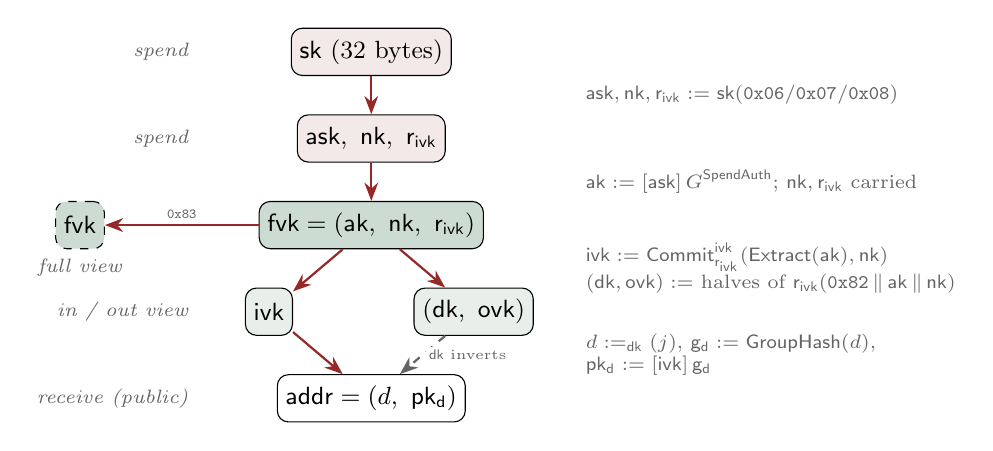
\begin{tikzpicture}[font=\small, x=1cm, y=1cm,
  k/.style={draw, rounded corners, inner sep=3pt, minimum height=6mm,
            anchor=center, fill=arb!10},
  kspend/.style={k, fill=arbred!10},
  kfull/.style={k, fill=arb!22},
  kpub/.style={k, fill=white},
  kint/.style={k, dashed, fill=arb!22},
  tier/.style={font=\scriptsize\itshape, text=arbdim, anchor=east},
  op/.style={font=\scriptsize, text=arbdim, anchor=west, align=left},
  elab/.style={font=\tiny, text=arbdim, inner sep=1pt, fill=white},
  ow/.style={-{Stealth}, thick, arbred},
  inv/.style={-{Stealth}, thick, arbdim, dashed}]
\node[kspend] (sk)    at (0,0)       {$\mathsf{sk}$ (32 bytes)};
\node[kspend] (mid)   at (0,-1.1)    {$\asksym,\ \nksym,\ \rivk$};
\node[kfull]  (fvk)   at (0,-2.2)    {$\fvk = (\aksym,\ \nksym,\ \rivk)$};
\node[kint]   (int)   at (-3.7,-2.2) {$\wbDint{\fvk}$};
\node[k]      (ivk)   at (-1.3,-3.3) {$\ivk$};
\node[k]      (dkovk) at (1.3,-3.3)  {$(\dk,\ \ovk)$};
\node[kpub]   (addr)  at (0,-4.4)    {$\mathsf{addr} = (d,\ \pkd)$};
\draw[ow] (sk)  -- (mid);
\draw[ow] (mid) -- (fvk);
\draw[ow] (fvk) -- (ivk);
\draw[ow] (fvk) -- (dkovk);
\draw[ow] (fvk) -- node[elab, above=1pt]{$\mathtt{0x83}$} (int);
\draw[ow] (ivk) -- (addr);
\draw[inv] (dkovk) -- node[elab, right=1pt]{$\dk$ inverts} (addr);
\node[op] at (2.6,-0.55)
  {$\asksym, \nksym, \rivk := \wbDprf{\mathsf{sk}}
   (\mathtt{0x06} / \mathtt{0x07} / \mathtt{0x08})$};
\node[op] at (2.6,-1.65)
  {$\aksym := [\asksym]\,G^{\mathsf{SpendAuth}}$; $\nksym, \rivk$ carried};
\node[op] at (2.6,-2.75)
  {$\ivk := \CommitIvk_{\rivk}(\Extract(\aksym), \nksym)$\\
   $(\dk, \ovk) :=$ halves of
   $\wbDprf{\rivk}(\mathtt{0x82}\,\|\,\aksym\,\|\,\nksym)$};
\node[op] at (2.6,-3.85)
  {$d := \wbDff_{\dk}(j)$, $\gd := \GroupHash(d)$,\\
   $\pkd := [\ivk]\,\gd$};
\node[tier] at (-2.2,0)    {spend};
\node[tier] at (-2.2,-1.1) {spend};
\node[tier, anchor=north] at (int.south) {full view};
\node[tier] at (-2.2,-3.3) {in / out view};
\node[tier] at (-2.2,-4.4) {receive (public)};
\end{tikzpicture}}

% d_keys.py: seed 32..252 bytes, >= 256 bits entropy; sk 32 bytes = 256 bits
% d_keys.py: hardened offset 2^31 = 2147483648; purpose 32' = 0x80000020
%   (shielded), 44' (transparent); coin type 133; accounts 0..2147483647
% d_keys.py: PRFexpand leads: spend 0x06/0x07/0x08, dk|ovk 0x82, internal
%   0x83, CKD 0x81; path levels below master: 3 (all hardened)
% d_keys.py: transparent path: 5 levels below master, 2 non-hardened;
%   Orchard path: 3 levels, all hardened
\begin{board}{BIP-32 becomes ZIP-32: one seed, two trees}{authorised}
\Write
\begin{enumerate}
  \item one seed: $32$--$252$ bytes, at least $256$ bits of entropy
  \item $(\mathsf{sk}_i, c_i) := \text{halves of }
    \wbDprf{c_{\mathrm{par}}}\bigl(\mathtt{0x81}\,\|\,
    \mathsf{sk}_{\mathrm{par}}\,\|\,i\bigr)$, \quad $i \ge 2^{31}$
  \item transparent:
    $m/44'/133'/\mathit{account}'/\mathit{change}/\mathit{index}$ ---
    two lowest levels non-hardened, xpub at the account
  \item Orchard: $m_{\mathsf{Orchard}}/32'/133'/\mathit{account}'$ ---
    hardened only, chain code discarded at the account, no change level
\end{enumerate}
\Say
\textbf{One seed roots both trees, as one BIP-32 seed roots a Bitcoin
wallet.} A seed of 32 to 252 bytes with at least 256 bits of entropy
roots the transparent tree and the shielded tree, so one backup recovers
every key.

\textbf{Transparent keys keep BIP-44 as the room knows it.} The path is
\[
m/44'/133'/\mathit{account}'/\mathit{change}/\mathit{index},
\]
the two lowest levels non-hardened, an xpub at the account.

\textbf{Orchard keys stop at the account, and every level is hardened.}
Each level applies the formula on the board; the chain code is discarded
at the account. The xpub mode --- a public key deriving child public keys
--- is undefined, so no Orchard extended full viewing key exists.

\textbf{Emphasise: there is no change level.} BIP-44's change branch
separates addresses on a public graph. A shielded change output is
indistinguishable on chain from any other output, so a change subtree
would separate nothing. Where change goes instead is the next two boards.
\src{\emph{Wallet Guide}, ``Wallet seeds''; ``Hardened-only derivation'';
``The standard account path''; ZIP-32, ``Key path levels''}
\end{board}

% d_keys.py: PRFexpand leads: spend 0x06/0x07/0x08, dk|ovk 0x82, internal
%   0x83, CKD 0x81; path levels below master: 3 (all hardened)
% ep_actions.py: amounts: in 200000000 -> Bob 150000000, change 49990000
%   zatoshi (0.4999 ZEC)
\begin{board}{Two scopes per account: external and internal}{authorised}
\Write
\begin{enumerate}
  \item $\wbDint{\rivk} := \mathrm{ToScalar}\bigl(\wbDprf{\rivk}(
    \mathtt{0x83}\,\|\,\aksym\,\|\,\nksym)\bigr)$
  \item $\wbDint{\fvk} := (\aksym,\ \nksym,\ \wbDint{\rivk})$
  \item same \asksym{} spends, same \nksym{} nullifies;
    \ivk, \dk, \ovk{} re-derived
  \item $\fvk \to \wbDint{\fvk}$; \quad $(\dk, \ivk) \to$ external scope
    only
\end{enumerate}
\Say
\textbf{Only \rivk{} changes.} The map $\mathrm{ToScalar}$ reduces the
$512$-bit PRF output modulo the Pallas scalar-field order. The same
\asksym{} spends and the same \nksym{} nullifies in both scopes; \ivk,
\dk{} and \ovk{} are re-derived, so an internal address does not decrypt
under the external \ivk.

\textbf{The internal key follows from the full viewing key.} A full
viewing key sees both scopes. An external $(\dk, \ivk)$ --- a payment
processor --- sees the external scope only, never the change: neither the
internal scope nor any \ovk{} follows from it.

\textbf{The Bitcoin contrast.} BIP-44 separates change by a path level on
a public graph; here the separation is a second full viewing key, and the
change output looks like any other output on chain.
\Avoid
\begin{itemize}
  \item ``The wallet recovers its change through \ovk.'' Change is a note
    to an internal address; the full viewing key sees it because
    $\wbDint{\fvk}$ follows from \fvk, and the internal \ivk{} decrypts it.
  \item ``The pair $(\dk, \ovk)$ comes from \ivk.'' No \ovk{} follows
    from $(\dk, \ivk)$; the pair comes from \fvk{} (the ladder board).
\end{itemize}
\src{\emph{Wallet Guide}, ``Internal keys: change and auto-shielding'';
ZIP-32, ``Orchard internal key derivation''; ZIP-316, ``Deriving Internal
Keys''}
\end{board}

% ep_actions.py: amounts: in 200000000 -> Bob 150000000, change 49990000
%   zatoshi (0.4999 ZEC)
\begin{board}{The internal scope: change and auto-shielding}{authorised}
\Write
\begin{enumerate}
  \item internal addresses $\leftarrow$ change, auto-shielded funds
  \item shielding $=$ moving transparent funds into the pool
    (automatic, to an internal address)
  \item Alice's change: $0.4999$ ZEC $\to$ internal address, index $0$
\end{enumerate}
\Say
\textbf{What BIP-44 puts in the path sits here in the key.} Internal
addresses take change and auto-shielded funds.

\textbf{Define shielding before using the word.} Shielding is moving
transparent funds into the pool; wallets do it automatically, to an
internal address.

\textbf{The running example.} The deployed wallet library (librustzcash)
sends change to the internal address at index $0$: Alice's $0.4999$ ZEC
goes there.

\textbf{The Bitcoin contrast.} A Bitcoin change output sits on the
change branch of a public graph; here the change output is
indistinguishable from any other, and only the internal scope's keys
find it.
\Avoid
\begin{itemize}
  \item ``Change is recovered via \ovk.'' Change is an incoming note to
    the internal address, seen through the internal scope, not through
    the outgoing key.
\end{itemize}
\src{\emph{Wallet Guide}, ``Internal keys: change and auto-shielding'';
\emph{Ironwood Guide}, ``The doors: shielding, coinbase, migration''}
\end{board}

% d_keys.py: sk 32 bytes; PRFexpand leads: spend 0x06/0x07/0x08, dk|ovk
%   0x82, internal 0x83
% d_keys.py: PRFexpand output 512 bits = 64 bytes; dk = first 32 bytes,
%   ovk = last 32 bytes
\begin{board}{The ladder: one secret, graded capabilities}
  {authorised / not twice}
\xdef\wbDLadderBoard{\theboard}%
\Draw
\begin{enumerate}
  \item A column of three boxes down the middle, top to bottom:
    ``$\mathsf{sk}$ (32 bytes)''; ``$\asksym, \nksym, \rivk$'';
    ``$\fvk = (\aksym, \nksym, \rivk)$''.
  \item Under \fvk, two boxes side by side: \ivk{} on the left,
    $(\dk, \ovk)$ on the right; under those, centred, a white box
    ``$\mathsf{addr} = (d, \pkd)$''.
  \item A dashed box ``$\wbDint{\fvk}$'' to the left of \fvk.
  \item Red arrows, one-way: $\mathsf{sk} \to$ middle box $\to \fvk$;
    $\fvk \to \ivk$; $\fvk \to (\dk, \ovk)$; $\ivk \to \mathsf{addr}$;
    and $\fvk \to \wbDint{\fvk}$ leftwards, labelled $\mathtt{0x83}$.
  \item One grey dashed arrow $(\dk, \ovk) \to \mathsf{addr}$, labelled
    ``\dk{} inverts''.
  \item Tier labels in the left margin: \emph{spend} beside the top two
    boxes; \emph{full view} under $\wbDint{\fvk}$; \emph{in / out view}
    beside the \ivk{} row; \emph{receive (public)} beside the address.
  \item The operation beside each rung, from Write below.
\end{enumerate}
\begin{center}
\resizebox{0.6\textwidth}{!}{\wbDLadderFig}
\end{center}
\Write
\begin{enumerate}
  \item $\asksym, \nksym, \rivk := \wbDprf{\mathsf{sk}}
    (\mathtt{0x06} / \mathtt{0x07} / \mathtt{0x08})$
  \item $\aksym := [\asksym]\,G^{\mathsf{SpendAuth}}$; \ $\nksym, \rivk$
    carried
  \item $\ivk := \CommitIvk_{\rivk}(\Extract(\aksym), \nksym)$
  \item $(\dk, \ovk) :=$ halves of
    $\wbDprf{\rivk}(\mathtt{0x82}\,\|\,\aksym\,\|\,\nksym)$
  \item $d := \wbDff_{\dk}(j)$, \ $\gd := \GroupHash(d)$, \
    $\pkd := [\ivk]\,\gd$
\end{enumerate}
\Say
\textbf{Red arrows are one-way.} A rung is handed down without the powers
above it.

\textbf{In Bitcoin, BIP-32 has two rungs, xprv and xpub, and the public
ledger supplies the rest.} Here every rung between is a separate secret
--- full view, incoming view, outgoing view --- and only the address at
the bottom is public.

\textbf{Emphasise: $(\dk, \ovk)$ come from \fvk{} by a PRF, not from
\ivk.} Point at the two downward arrows leaving \fvk: the \ivk{} branch
and the
$(\dk, \ovk)$ branch are siblings.

\textbf{The circuit re-walks $\fvk \to \ivk \to \pkd$ (A7) with \gd{} as
a witness.} The step $j \to d \to \gd$ that produces the witness is
never checked in the circuit; that is the dashed grey edge, and the
diversified-addresses board says why.
\Avoid
\begin{itemize}
  \item ``The pair $(\dk, \ovk)$ is derived from \ivk.'' Both branches
    leave \fvk; the incoming viewing key yields neither.
\end{itemize}
\src{\emph{Ironwood Guide}, ``The capability ladder''; ``Viewing keys'';
``The Action statement, formally''; protocol specification, ``Orchard Key
Components''}
\end{board}

% d_keys.py: PRFexpand leads: spend 0x06/0x07/0x08, dk|ovk 0x82, internal
%   0x83
\begin{board}{What holds the rungs apart}{authorised / not twice}
\Draw
Three columns --- \emph{step} $\mid$ \emph{operation} $\mid$ \emph{why it
is one-way} --- one row at a time:
\begin{enumerate}
  \item $\mathsf{sk} \to (\asksym, \nksym, \rivk)$ $\mid$
    $\wbDprf{\mathsf{sk}}(\mathtt{0x06}/\mathtt{0x07}/\mathtt{0x08})$
    $\mid$ PRF (BLAKE2b)
  \item $\asksym \to \aksym$ $\mid$ $[\asksym]\,G^{\mathsf{SpendAuth}}$
    $\mid$ discrete log on Pallas
  \item $\fvk \to \ivk$ $\mid$ $\CommitIvk_{\rivk}(\Extract(\aksym),
    \nksym)$ $\mid$ hiding under \rivk
  \item $\fvk \to (\dk, \ovk)$ $\mid$ halves of
    $\wbDprf{\rivk}(\mathtt{0x82}\,\|\,\aksym\,\|\,\nksym)$ $\mid$ PRF
  \item $\fvk \to \wbDint{\fvk}$ $\mid$
    $\wbDprf{\rivk}(\mathtt{0x83}\,\|\,\aksym\,\|\,\nksym)$ $\mid$ PRF
  \item $\ivk \to \pkd$ $\mid$ $[\ivk]\,\gd$ $\mid$ discrete log on Pallas
  \item $j \to d$ $\mid$ $\wbDff_{\dk}(j)$ $\mid$ \emph{not} one-way:
    \dk{} inverts it
\end{enumerate}
\Write
\begin{enumerate}
  \item the scalar \ivk: a commitment, not a hash --- binds \emph{and}
    hides $(\aksym, \nksym)$
  \item one \rivk{} keys both $\CommitIvk$ and the $\mathtt{0x82}$ PRF
    $\Rightarrow$ joint assumption once \dk{} or \ovk{} is exposed
  \item a separate \nksym: spent status without spend authority
\end{enumerate}
\Say
\textbf{Three kinds of wall.} A PRF (BLAKE2b) at the top and at the
$\mathtt{0x82}$ and $\mathtt{0x83}$ splits; a discrete logarithm on
Pallas at $\asksym \to \aksym$ and at $\ivk \to \pkd$; a hiding
commitment at $\fvk \to \ivk$.

\textbf{The scalar \ivk{} is a commitment, not a hash, because it must
bind and hide $(\aksym, \nksym)$.} An \ivk{} holder learns neither. Since
\rivk{} also keys the $\mathtt{0x82}$ PRF, hiding rests on a joint
assumption once \dk{} or \ovk{} is exposed.

\textbf{Why a separate \nksym.} Spent status can be delegated without
spend authority: the viewing key holds \nksym, never \asksym.

\textbf{The last row is deliberately not one-way.} The diversifier key
inverts FF1, so the \dk{} holder maps any of its addresses back to an
index. Bitcoin has one wall, xprv to xpub; the rest of its ladder is
public.
\Avoid
\begin{itemize}
  \item ``The pair $(\dk, \ovk)$ comes from \ivk.'' Row~4 starts at
    \fvk.
\end{itemize}
\src{\emph{Ironwood Guide}, ``The capability ladder''; \emph{Wallet Guide},
``Diversified addresses''; protocol specification, ``Orchard Key
Components''}
\end{board}

\begin{board}{Graded capabilities: spend, full view, spent status}
  {authorised / not twice}
\Draw
Four columns --- \emph{capability} $\mid$ \emph{holds} $\mid$ \emph{can}
$\mid$ \emph{cannot} --- one row at a time:
\begin{enumerate}
  \item spend $\mid$ \asksym{} (from $\mathsf{sk}$) $\mid$ authorise
    spends, both scopes $\mid$ ---
  \item full view $\mid$ $\fvk = (\aksym, \nksym, \rivk)$ $\mid$
    everything below, both scopes; every address and its index $\mid$
    spend: \asksym{} is a discrete log away
  \item spent status $\mid$ \nksym{} (inside \fvk) $\mid$ the nullifier
    of a note it holds $\mid$ spend; find notes (needs \ivk)
\end{enumerate}
\Write
\begin{enumerate}
  \item Bitcoin: only the spend row is secret (xprv)
\end{enumerate}
\Say
\textbf{Each row holds strictly less than the one above.} Spend authority
is \asksym, from $\mathsf{sk}$, and it covers both scopes. Full view is
\fvk: everything below it, both scopes, every address and its index ---
but not spending, because \asksym{} is a discrete logarithm away from
\aksym. Spent status is \nksym{} alone: it computes the nullifier of a
note it is handed, and can neither spend nor find notes, which needs
\ivk.

\textbf{Bitcoin keeps only the spend row secret (xprv).} Full view and
spent status are what its public ledger shows to everyone.

\textbf{Emphasise the middle row.} A full viewing key sees everything and
moves nothing.
\src{\emph{Ironwood Guide}, ``The capability ladder''; \emph{Wallet Guide},
``From the account key to addresses: the layer already built''}
\end{board}

% d_keys.py: diversifier 88 bits; addresses per account per scope 2^88
\begin{board}{Graded capabilities: incoming, outgoing, receive}{exists}
\Draw
Same four columns, three more rows:
\begin{enumerate}
  \item incoming view $\mid$ $(\dk, \ivk)$ $\mid$ detect and decrypt
    incoming; derive all $2^{88}$ addresses and invert them to indices
    $\mid$ nullifiers, so spent status; outgoing; the internal scope
  \item outgoing view $\mid$ \ovk{} $\mid$ open $C_{\mathrm{out}}$ of
    what this account and scope sent (a sender may set $\ovk = \bot$:
    then no \ovk{} opens it) $\mid$ incoming; the internal \ovk
  \item receive $\mid$ $(d, \pkd)$ $\mid$ be paid $\mid$ anything else
    --- the only public item
\end{enumerate}
\Write
\begin{enumerate}
  \item every row but the last is a distinct secret
\end{enumerate}
\Say
\textbf{Every row but the last is a distinct secret.} Bitcoin's ledger
collapses everything between xprv and the address into what anyone can
read.

\textbf{The incoming view sees arrivals, not departures.} The pair
$(\dk, \ivk)$ detects and decrypts incoming notes and enumerates all
$2^{88}$ addresses, inverting each to its index; it has no nullifiers,
so no spent status, no outgoing view, and no internal scope.

\textbf{The outgoing view may open nothing.} The key \ovk{} opens
$C_{\mathrm{out}}$ of what this account and scope sent, but a sender may
set $\ovk = \bot$, and then no \ovk{} opens it.

\textbf{Emphasise: the address is the only public item.} It lets one be
paid and does nothing else.
\Avoid
\begin{itemize}
  \item ``The pair $(\dk, \ovk)$ comes from \ivk.'' The incoming row
    holds no \ovk{} and cannot reach one.
\end{itemize}
\src{\emph{Ironwood Guide}, ``The capability ladder''; ``The outgoing
ciphertext''; \emph{Wallet Guide}, ``Raw encodings''; ZIP-316, ``Deriving
Internal Keys''}
\end{board}

\begin{board}{Viewing keys: xpub is the bridge, not the analogue}
  {exists / not twice}
\Write
\begin{enumerate}
  \item xpub $=$ watch-only: enumerates addresses; the public ledger
    supplies incoming, outgoing, spent status --- to anyone
  \item $(\dk, \ivk)$ $=$ watch-only for incoming: enumerates \emph{and}
    decrypts
  \item three differences: (1) nothing visible without the key;
    (2) spent status $=$ \nksym; (3) outgoing $=$ \ovk
  \item ``viewing'' $=$ a capability, not publicity
\end{enumerate}
\Say
\textbf{Start from what the room has: an xpub is a watch-only wallet.} It
enumerates the addresses, and the public ledger supplies incoming,
outgoing and spent status --- to anyone, xpub or not.

\textbf{The pair $(\dk, \ivk)$ is the watch-only wallet for incoming.} It
enumerates the addresses \emph{and} decrypts. Then the three differences,
in order: Bitcoin shows everything regardless, here nothing is visible
without the key, because the outputs are ciphertext; spent status is a
second secret, \nksym, which computes the nullifiers that the chain's
set is matched against; outgoing is a third, \ovk, which opens
$C_{\mathrm{out}}$. The xpub gets both free only because Bitcoin's ledger
is public.

\textbf{Emphasise: ``viewing'' names a capability, not publicity.} Every
viewing key is secret material disclosed deliberately --- to an auditor,
a processor --- and validation needs none of them.
\Avoid
\begin{itemize}
  \item ``The pool is auditable.'' A viewing key discloses one account,
    to whoever its holder chooses; nothing about the pool is readable
    without one, and the validator holds none.
\end{itemize}
\src{\emph{Ironwood Guide}, ``The capability ladder''; ``What a node
verifies, without ever observing the note''; \emph{Wallet Guide},
``Unified viewing keys''}
\end{board}

% d_keys.py: diversifier 88 bits; addresses per account per scope
%   2^88 = 309485009821345068724781056 ~ 3.1e+26; random draws collide near
%   2^44 = 17592186044416
% d_keys.py: raw receiver 11 + 32 = 43 bytes
\begin{board}{Diversified addresses: one key, $2^{88}$ addresses}{exists}
\Write
\begin{enumerate}
  \item $d := \wbDff_{\dk}(j)$
  \item $\gd := \wbDgh$
  \item $\pkd := [\ivk]\,\gd$, \quad $\mathsf{addr} := (d,\ \pkd)$
  \item $2^{88} \approx 3.1 \times 10^{26}$ addresses per key;
    raw receiver $11 + 32 = 43$ bytes
  \item random $88$-bit draws collide near $2^{44}$; FF1 never collides,
    and \dk{} inverts it
\end{enumerate}
\Say
\textbf{Every index works.} Each $j$ of the $2^{88} \approx 3.1 \times
10^{26}$ gives an address: $\GroupHash$ is total (a fixed fallback covers
the identity), so there is no rejection loop. A raw receiver is
$11 + 32 = 43$ bytes, and all of them are spent by one \asksym{} and
found by one \ivk, at no extra scanning cost.

\textbf{A keyed permutation, not a counter and not a hash.} Consecutive
indices scatter over $\{0,1\}^{88}$ and never collide --- random 88-bit
draws would, near $2^{44}$ --- and \dk{} inverts the map, so the wallet
stores nothing per address.

\textbf{Wallet-side only, never in the circuit.} That is why AES is fine
here: the circuit takes \gd{} as a witness (Board~\wbDLadderBoard) and never
sees $j$.

\textbf{The Bitcoin contrast.} An xpub also enumerates addresses; the
difference is what an address reveals, which is the next board.
\src{\emph{Ironwood Guide}, ``Diversified addresses''; \emph{Wallet Guide},
``Diversified addresses''; ``Raw encodings''; \emph{Crypto Guide},
``Format-preserving encryption and FF1''; ZIP-32, ``Orchard key path''}
\end{board}

% d_keys.py: diversifier 88 bits; addresses per account per scope 2^88
\begin{board}{Unlinkable, even to the payer}{exists}
\Write
\begin{enumerate}
  \item $(d, \pkd)$ and $(d', \pkd')$: \ $\pkd = [\ivk]\,\gd$,
    \ $\pkd' = [\ivk]\,\gd'$ \ --- same \ivk?
  \item deciding it $=$ DDH on Pallas, $\GroupHash$ a random oracle
  \item only $(\dk, \ivk)$ can check: re-derive at the decrypted index
  \item never a chosen-diversifier oracle
\end{enumerate}
\Say
\textbf{Two addresses, one question: same \ivk?} Deciding it is a DDH
problem on Pallas with $\GroupHash$ as a random oracle: given two
addresses of different owners and a third derived from one of them, no
one can tell which. Alice, who paid one of Bob's addresses, learns
nothing about the other.

\textbf{Only the holder of $(\dk, \ivk)$ can check}, by re-deriving the
address at the decrypted index under that \ivk.

\textbf{One rule for implementers.} Never offer a chosen-diversifier
oracle --- an address for an attacker's $d$ under your \ivk: it breaks
unlinkability for every address of that \ivk.

\textbf{The Bitcoin contrast, and the thing to emphasise.} Under one
xpub, addresses link on the public graph once spent together (Part~A),
and a leaked xpub links all beneath it, spent or not. Here an address
reveals only itself.
\src{\emph{Wallet Guide}, ``Diversified addresses''; \emph{Ironwood Guide},
``Diversified addresses''; protocol specification,
``$\mathsf{DiversifyHash}^{\mathsf{Sapling}}$ and
$\mathsf{DiversifyHash}^{\mathsf{Orchard}}$ Hash Functions''}
\end{board}

% d_keys.py: typecodes: 0x00 P2PKH, 0x01 P2SH, 0x02 Sapling, 0x03 Orchard;
%   priority = descending typecode
\begin{board}{Unified addresses (ZIP-316): one string, several receivers}
  {exists}
\Write
\begin{enumerate}
  \item typecodes: $\mathtt{0x00}$ P2PKH, $\mathtt{0x01}$ P2SH,
    $\mathtt{0x02}$ Sapling, $\mathtt{0x03}$ Orchard --- at most one
    each, at least one shielded
  \item ascending typecode $\to$ F4Jumble (whole payload, HRP included)
    $\to$ Bech32m
  \item sender: Orchard $>$ Sapling $>$ transparent; may refuse a type,
    never reorder
  \item Orchard receiver $\to$ the Ironwood pool
\end{enumerate}
\Say
\textbf{One string carries at most one receiver per type, with at least
one shielded.} Transparent P2PKH or P2SH ($\mathtt{0x00}$ /
$\mathtt{0x01}$), Sapling ($\mathtt{0x02}$), Orchard ($\mathtt{0x03}$).
Items are encoded in ascending typecode, passed through F4Jumble --- an
unkeyed four-round Feistel permutation of the whole payload, HRP included
--- then Bech32m, so a substituted receiver changes the whole string, not
one region of it.

\textbf{What a sender does.} Use the most preferred receiver it supports:
Orchard over Sapling over transparent. A wallet may refuse a type, never
reorder.

\textbf{Which pool.} An Orchard receiver names the protocol, not a pool,
and all new value enters the Ironwood pool, so a payment to it lands in
the Ironwood tree; the receiver has no string form of its own.

\textbf{The same container with viewing-key items} is a unified full or
incoming viewing key.

\textbf{The Bitcoin contrast.} One Bitcoin address encodes one script
type; here one address lets the sender's wallet choose the pool.
\src{\emph{Wallet Guide}, ``Unified addresses''; ``String encoding:
F4Jumble and Bech32m''; ``Unified viewing keys''; \emph{Ironwood Guide},
``One ladder, both pools''; ZIP-316, ``Encoding of Unified Addresses''}
\end{board}

% d_keys.py: Bob receives 1.5 ZEC = 150000000 zatoshi; Ironwood lead byte
%   0x03; raw receiver 11 + 32 = 43 bytes
% ep_actions.py: amounts: in 200000000 -> Bob 150000000, change 49990000
%   zatoshi (0.4999 ZEC)
% d_keys.py: PRFexpand leads: spend 0x06/0x07/0x08, dk|ovk 0x82, internal
%   0x83
\begin{board}{Bob's address in the example}{exists}
\Write
\begin{enumerate}
  \item $\mathsf{addr}_B = (d_B,\ \pkd)$, $43$ bytes
  \item $\gd := \GroupHash^{\Pallas}(\mathtt{z.cash:Orchard\text{-}gd},\
    d_B)$, \quad $\epk := [\esk]\,\gd$
  \item $\mathbf{n} := (\mathsf{addr}_B,\ 1.5\ \text{ZEC},\ \rho,\ \psi,\
    \rcm)$
  \item on chain: inside \cmsym, inside $C_{\mathrm{enc}}$, as \epk{}
    under a fresh \esk; lead byte $\mathtt{0x03}$
  \item change $0.4999$ ZEC $\to$ Alice's internal address, index $0$
\end{enumerate}
\Say
\textbf{Bob hands Alice a unified address; her wallet takes its Orchard
receiver.} That is $\mathsf{addr}_B = (d_B, \pkd)$, 43 bytes. From it she
derives \gd, then \epk{} under a fresh \esk, and builds the note
$\mathbf{n}$ with $1.5$ ZEC.

\textbf{That is all it learns.} No \ivk, \nksym{} or \aksym, no index
$j$, no link to Bob's other addresses. On chain the address appears only
blinded: inside \cmsym, inside $C_{\mathrm{enc}}$, and as \epk{} under a
fresh \esk.

\textbf{Which tree.} The note is minted in the Ironwood tree, lead byte
$\mathtt{0x03}$; Bob's one \ivk{} trial-decrypts both pools.

\textbf{Her change, $0.4999$ ZEC, goes to her internal address at index
$0$}: no address of hers appears either.

\textbf{The Bitcoin contrast.} Bitcoin displays the script beside the
amount; here neither appears in the clear.
\Ask
Which key does an accountant need to audit a company's incoming
\emph{and} outgoing shielded payments --- and what can they not do with
it?
\begin{itemize}
  \item One unified full viewing key per account. Inside it, \fvk{}
    yields \ivk{} (incoming), \nksym{} (which of those notes are spent)
    and \ovk{} (outgoing) --- for the external scope and, through the
    $\mathtt{0x83}$ step, the internal one, so change is covered too.
  \item Not spend: \asksym{} is a discrete logarithm away from \aksym.
    Not wander into a sibling account: only hardened derivation exists,
    and no Orchard extended full viewing key.
  \item Not read what was sent under some other \ovk, or under none: the
    sender may set $\ovk = \bot$, and then no \ovk{} opens
    $C_{\mathrm{out}}$. Nor anything received by an account they were
    not given.
\end{itemize}
\Avoid
\begin{itemize}
  \item ``The proof hides the receiver.'' The commitment, the ciphertext
    and the fresh \esk{} blind the address; the proof shows the address
    was used consistently (A7).
  \item ``The pair $(\dk, \ovk)$ comes from \ivk.'' The accountant's
    \ovk{} comes from \fvk.
  \item ``Change is recovered via \ovk.'' Change is an incoming note in
    the internal scope; the full viewing key covers it through the
    $\mathtt{0x83}$ step.
\end{itemize}
\src{\emph{Ironwood Guide}, ``Sender: one-shot Diffie--Hellman and the
AEAD''; ``The note and its commitment''; ``One ladder, both pools''; ``The
capability ladder''; ``The outgoing ciphertext''; \emph{Wallet Guide},
``Unified addresses''; ``Internal keys: change and auto-shielding'';
``From the account key to addresses: the layer already built'';
``Unified viewing keys''}
\end{board}

%% ---- 05-statement.tex
%% ---- Part E --- The Action statement: whiteboard companion
\newcommand{\wbEcv}{\ensuremath{\cvsym^{\mathsf{net}}}}
\newcommand{\wbEnf}{\ensuremath{\nfsym_{\mathrm{old}}}}
\newcommand{\wbEanc}{\ensuremath{\mathsf{anchor}}}
\newcommand{\wbEold}[1]{\ensuremath{#1_{\mathrm{old}}}}
\newcommand{\wbEnew}[1]{\ensuremath{#1_{\mathrm{new}}}}
\newcommand{\wbEcenc}{\ensuremath{C_{\mathrm{enc}}}}
\newcommand{\wbEcout}{\ensuremath{C_{\mathrm{out}}}}
\newcommand{\wbEflag}[1]{\ensuremath{\mathsf{#1}}}
\newcommand{\wbEPoseidon}{\ensuremath{\mathsf{Poseidon}}}
\newcommand{\wbEgsa}{\ensuremath{G^{\mathsf{SpendAuth}}}}
\newcommand{\wbEgnf}{\ensuremath{G^{\mathsf{nf}}}}
% \wbEActionBox[field]: the deck's \ActionBox, one Action inside its bundle;
% field in {none, anchor, nf, cv, rk, cmx, proof} is drawn highlighted.
\newcommand{\wbEActionBox}[1][none]{%
  \tikzset{wbEhlnone/.style={}, wbEhlanchor/.style={}, wbEhlnf/.style={},
    wbEhlcv/.style={}, wbEhlrk/.style={}, wbEhlcmx/.style={},
    wbEhlproof/.style={},
    wbEhl#1/.style={draw=arbred, very thick, fill=arbred!15}}%
  \begin{tikzpicture}[font=\scriptsize, x=1cm, y=1cm,
    ebox/.style={draw=black!60, fill=white, rounded corners=2pt,
      inner sep=2.5pt, align=center},
    elab/.style={inner sep=2pt, text=black!60}]
  % the bundle; a second Action behind the first
  \draw[draw=black!50, dashed, rounded corners=3pt]
    (-2.45,-2.45) rectangle (4.75,2.5);
  \node[elab, anchor=north west, text=black!70, font=\scriptsize\bfseries]
    at (-2.45,2.5) {bundle};
  \draw[draw=arb!40, rounded corners=3pt] (-2.0,-2.1) rectangle (2.4,2.1);
  \node[elab, anchor=south east, text=arb!60] at (2.4,2.1) {$\times\,n$};
  \node[draw=arb, thick, fill=white, rounded corners=3pt,
    minimum width=4.4cm, minimum height=3.9cm] (act) at (0,0) {};
  \node[anchor=north west, font=\scriptsize\bfseries, text=arb,
    inner sep=2pt] at (act.north west) {Action};
  \node[draw=arb!60, fill=arb!8, rounded corners=2pt, inner sep=3pt,
    align=center, anchor=north, text width=3.8cm] (wit) at (0,1.62)
    {\textbf{witness} --- never published\\
     old note, new note\\
     Merkle path $+$ position\\
     $\aksym, \nksym, \rivk, \ivk$; $\alpha$, $\rcv$};
  \node[elab, anchor=west] at (-2.15,-0.12) {public, per Action};
  \node[ebox, wbEhlcv, anchor=west] (cv) at (-2.05,-0.58) {$\wbEcv$};
  \node[ebox, wbEhlnf, right=1.2mm of cv] (nf) {$\wbEnf$};
  \node[ebox, wbEhlrk, right=1.2mm of nf] (rk) {$\rksym$};
  \node[ebox, wbEhlcmx, right=1.2mm of rk] (cmx) {$\cmx$};
  \node[ebox, draw=black!40, dashed] (ct) at (0,-1.15)
    {$\epk,\ \wbEcenc,\ \wbEcout$};
  \node[elab, align=center, font=\tiny, text=black!60] at (0,-1.66)
    {delivery ciphertexts --- no in-circuit check;\\
     opened only with $\ivk$/$\ovk$ (\emph{Delivery})};
  % bundle-level fields
  \node[ebox, wbEhlanchor, anchor=west] (anc) at (2.45,1.65) {$\wbEanc$};
  \node[ebox, anchor=west] (flg) at (2.45,1.0) {flags};
  \node[ebox, anchor=west] (vb)  at (2.45,0.35) {$v_{\mathrm{balance}}$};
  \node[ebox, wbEhlproof, anchor=west] (prf) at (2.45,-0.3) {proof};
  \node[ebox, anchor=west] (sas) at (2.45,-0.95) {SpendAuthSigs};
  \node[ebox, anchor=west] (bsg) at (2.45,-1.6) {binding sig};
  \end{tikzpicture}}

\section{Part E --- The Action statement}

\begin{board}{Anatomy of an Action}{all four}
\Draw
\begin{enumerate}
  \item A large dashed rectangle; write \emph{bundle} in its top-left
    corner.
  \item Inside, a solid box labelled \emph{Action} top-left, with a faint
    second box just behind it; write $\times\,n$ at that box's corner.
  \item Top of the Action box, a shaded block: \emph{witness --- never
    published}: old note, new note; Merkle path $+$ position;
    $\aksym, \nksym, \rivk, \ivk$; $\alpha$, $\rcv$.
  \item Below it, a row of four small boxes: $\wbEcv$, $\wbEnf$,
    $\rksym$, $\cmx$; label the row \emph{public, per Action}.
  \item Under the row, a dashed box: $\epk,\ \wbEcenc,\ \wbEcout$;
    caption it \emph{delivery ciphertexts --- no in-circuit check; opened
    only with $\ivk$/$\ovk$ (Delivery)}.
  \item Down the right edge, inside the bundle but outside the Action,
    six boxes top to bottom: $\wbEanc$, flags, $v_{\mathrm{balance}}$,
    proof, SpendAuthSigs, binding sig.
\end{enumerate}
\begin{center}\wbEActionBox\end{center}
\Write
\begin{itemize}
  \item one Action $=$ one old note spent $+$ one new note created
  \item witness (never published): old note, new note, path $+$
    position, $\aksym, \nksym, \rivk, \ivk$, $\alpha$, $\rcv$
  \item rim, per Action: $\wbEcv$, $\wbEnf$, $\rksym$, $\cmx$ --- the four
    the proof binds
  \item dashed: $\epk$, $\wbEcenc$, $\wbEcout$ --- ciphertexts, read by no
    clause
\end{itemize}
\Say
\textbf{Start from the shape.} One Action spends one old note and
creates one new one; the shape is fixed, so an Action never shows which
it ``really'' is.

\textbf{The witness stays inside.} Both notes, the path, the keys,
$\alpha$, $\rcv$ --- never published.

\textbf{Four fields on the rim are what the proof binds.} Per Action:
$\wbEcv$, $\wbEnf$, $\rksym$, $\cmx$.

\textbf{The dashed box is delivery, not verification.} The fields
$\epk$, $\wbEcenc$, $\wbEcout$ are ciphertexts read by no clause; only
$\ivk$ or $\ovk$ opens them (\emph{Delivery and light clients}).

\textbf{Bitcoin contrast.} A Bitcoin input names its coin and shows its
script; a Bitcoin output shows its amount and its script. Here every
field is a commitment, a serial number, a disguised key, or a
ciphertext.
\Avoid
``The proof hides the sender and receiver.'' The fields hide them ---
each is a commitment, a serial number, a disguised key, or a ciphertext;
the proof establishes the statement about them and nothing more.
\src{\emph{Ironwood Guide}, ``One Action, one payment: the walkthrough'';
``The outgoing ciphertext''; ``The Action statement, formally''}
\end{board}

\begin{board}{The bundle around it}{all four}
\Draw
Three columns: \emph{per bundle} $\mid$ \emph{once} $\mid$ \emph{role}.
Rows, in order:
\begin{enumerate}
  \item $\wbEanc$ --- one root, shared by every Action --- the tree the
    spends prove membership in
  \item flags --- $\wbEflag{enableSpends}$, $\wbEflag{enableOutputs}$,
    $\wbEflag{enableCrossAddress}$ --- consensus gates (A8--A10)
  \item $v_{\mathrm{balance}}$ --- signed, cleartext --- net value leaving
    the pool
  \item proof --- one aggregate Halo 2 proof --- covers all $n$ Actions at
    once
  \item binding sig --- one signature --- proves the values balance
  \item (a gap, then) per Action --- SpendAuthSig under $\rksym$ --- the
    owner authorised this spend
\end{enumerate}
\Write
\begin{itemize}
  \item one Action $= 820$ public bytes, $660$ of them ciphertext
  \item Alice: $2$ Actions, one $7264$-byte proof
  \item node checks: proof, anchor, nullifier set, two signatures ---
    never a note
\end{itemize}
\Say
\textbf{The bundle is written once; the Action is repeated.} One anchor
shared by every Action; three flags driving the consensus gates
A8--A10; a signed, cleartext $v_{\mathrm{balance}}$, the net value
leaving the pool; one aggregate Halo 2 proof covering all $n$ Actions
at once; one binding signature proving the values balance. Per Action,
one SpendAuthSig under $\rksym$: the owner authorised this spend.

\textbf{Sizes.} Each Action is $820$ public bytes, $660$ of them
ciphertext; Alice's bundle carries two Actions and one $7264$-byte
proof.

\textbf{What the node touches.} The node checks the proof, the anchor,
the nullifier set, and the two signatures --- and never sees a note.
Both signatures and $v_{\mathrm{balance}}$ return in \emph{Balance and
authority}.
\Avoid
``A few hundred bytes.'' Alice's proof is $7264$ bytes for two Actions,
and each Action adds $820$ public bytes.
\src{\emph{Ironwood Guide}, ``What a node verifies, without ever
observing the note''; ``The v6 transaction and the Ironwood component''}
\end{board}

\begin{board}{Why a spend and an output are fused}{all four}
\Write
\[
n_{\mathrm{act}}(s, o) = \max\bigl(\max(s, o),\, 2\bigr)
\qquad\text{Alice: } s = 1,\ o = 2 \;\Rightarrow\; n_{\mathrm{act}} = 2
\]
\begin{itemize}
  \item spend list and output list each padded to $n_{\mathrm{act}}$;
    floor $2$
  \item Alice: $1$ spend, $2$ outputs (Bob, change) $\Rightarrow$ one
    dummy spend
\end{itemize}
\Say
\textbf{A Bitcoin transaction shows its true input and output counts.}
Here the count is $n_{\mathrm{act}}$, and the fee is computed from that
public count (\emph{The transaction and the turnstile}).

\textbf{Uniformity.} Every Action looks like every other: one spend
slot, one output slot, whatever the payment needed.

\textbf{Padding.} The spend list and the output list are each extended
to $n_{\mathrm{act}}$; the floor is two. Alice's one spend and two
outputs (Bob, change) pad with one dummy spend.

\textbf{Scope.} This count, and the shuffle on the next board, are the
Ironwood component's (cross-address enabled). A sealed Orchard-pool
bundle pads to $s + o$ and pairs each spend with an output to the spent
note's own receiver.
\Avoid
``The dummy is there because of the minimum of two Actions.'' Alice's
$n_{\mathrm{act}} = 2$ comes from her two outputs; the dummy pads the
spend list up to that count. The floor of two is a separate rule that
gives the same number here.
\src{\emph{Wallet Guide}, ``Padding, dummies, and shuffling''; \emph{Ironwood
Guide}, ``Spending under the restriction''}
\end{board}

\begin{board}{Dummies and the shuffle}{all four}
\Write
\begin{itemize}
  \item dummy spend: value $0$, fresh random spending key,
    $\rho = \Extract(\text{random Pallas point})$; still publishes a
    nullifier
  \item dummy output: value $0$, fresh random address,
    $\rho := \wbEnf$ like any output's
  \item shuffle spends and outputs \emph{independently}, then zip
  \item Alice: spend side $\{2\text{ ZEC note}, \text{dummy}\}$; output
    side $\{\text{Bob}, \text{change}\}$
\end{itemize}
\Say
\textbf{A slot with nothing real in it holds a dummy.} A dummy spend is a
zero-value note under a fresh random spending key, its $\rho$ the
$\Extract$ of a random Pallas point; it still publishes a nullifier. A
dummy output is a zero-value note to a fresh random address, its
$\rho := \wbEnf$ like any output's.

\textbf{Shuffle, then zip.} Spends and outputs are shuffled
independently; which spend shares an Action with which output is
random.

\textbf{Alice's bundle.} Her $2$ ZEC note and a dummy on the spend side,
Bob's note and her change on the output side; which pair forms which
Action is the shuffle's choice.

\textbf{Bitcoin contrast.} A Bitcoin input is an input and an output is
an output; here a dummy spend looks exactly like a real one and, like a
real one, publishes a nullifier the pool records.
\Avoid
Writing $\rho$ as the note's position in the tree. The seed $\rho$ is a
per-note uniqueness value: a dummy's is the $\Extract$ of a random
point, an output's is the nullifier of the note spent beside it. Neither
is a leaf index.
\src{\emph{Wallet Guide}, ``Padding, dummies, and shuffling''; \emph{Ironwood
Guide}, ``The nullifier, and the loop back to minting''; protocol
specification, ``Dummy Notes (Orchard)''}
\end{board}

\begin{board}{The statement, in the validator's language}{all four}
\Write
\begin{itemize}
  \item \emph{``Some leaf under this anchor is a note I own; this is its
    serial number; this commitment hides its value change; this signing
    key is a fresh disguise of the owner's --- and I have shown you
    neither the leaf, the note, nor the owner's key.''}
  \item public: $\wbEanc$, $\wbEcv$, $\wbEnf$, $\rksym$, $\cmx$, three
    flags --- $8$ names, $10$ field elements
  \item witness: both notes, path $+$ position, $\aksym$, $\nksym$,
    $\rivk$, $\ivk$, $\alpha$, $\rcv$
  \item relation: ten clauses A1--A10; one verifying key, selected by
    branch; a proof of nine fails
\end{itemize}
\Say
\textbf{Say the statement in the validator's words first.} Read the
quoted sentence off the board.

\textbf{Public inputs.} The anchor, $\wbEcv$, $\wbEnf$, $\rksym$, $\cmx$
and the three flags --- eight names, ten field elements (the two Pallas
points enter by their coordinates). Here $\wbEcv$ and $\wbEnf$ are the
data model's $\cvsym$ and $\nfsym$, marked \emph{net} (this Action's
value change) and \emph{old} (the note spent).

\textbf{Witness.} Both notes, the path and position, $\aksym$, $\nksym$,
$\rivk$, $\ivk$, $\alpha$, $\rcv$.

\textbf{Relation.} Ten clauses, A1--A10, over those inputs. The node's
verifying key fixes exactly these ten, selected by branch; a proof of
nine is a proof for a different circuit, and it fails.

\textbf{Bitcoin contrast --- the one thing to emphasise.} Bitcoin's
validator runs \emph{your} script. This validator runs one verifier
keyed to one fixed circuit; the transaction supplies inputs, never
logic.
\src{\emph{Ironwood Guide}, ``The Action statement, formally''; ``One
circuit, one verifying key''; protocol specification, ``Action Statement
(Orchard)''}
\end{board}

\begin{board}{The ten clauses, ordered by the four checks}{all four}
\Draw
Three columns: \emph{Bitcoin's check} $\mid$ \emph{clause} $\mid$
\emph{what the proof establishes}. Rows, in order:
\begin{enumerate}
  \item coin exists (UTXO lookup) --- A3 --- a Merkle path from
    $\wbEold{\cmsym}$ to the anchor
  \item not spent twice (entry deleted) --- A5 --- $\wbEnf$ is this
    note's serial, keyed by $\nksym$
  \item conserved ($\sum\mathrm{in} \ge \sum\mathrm{out}$) --- A4 ---
    $\wbEcv$ hides $\wbEold{v} - \wbEnew{v}$, both below $2^{64}$
  \item authorised (script $+$ signature) --- A6, A7 --- $\rksym$
    disguises $\aksym$; $\aksym, \nksym$ sit behind the address
  \item (a gap, then) well-formed --- A1, A2 --- both commitments open
    to notes; $\wbEnew{\rho} = \wbEnf$
  \item gated --- A8, A9 --- spends and outputs switched on by the flags
  \item sealed --- A10 --- cross-address transfers switched off, or not
\end{enumerate}
\Write
\begin{itemize}
  \item $4$ Bitcoin checks $\to$ $7$ clauses (A1--A7); $3$ consensus
    gates (A8--A10)
  \item stays with the node: ``has this serial been seen?''
\end{itemize}
\Say
\textbf{Order the clauses by Bitcoin's checks, not by their numbers.}
Fill the top four rows first: existence is a Merkle path (A3), no
double spend is a keyed serial (A5), conservation is a hidden
difference in range (A4), authorisation is a disguised key behind the
address (A6, A7).

\textbf{Then the three rows below the gap.} Well-formed (A1, A2): both
commitments open to notes, and $\wbEnew{\rho} = \wbEnf$. Gated (A8,
A9): spends and outputs switched on by the flags. Sealed (A10):
cross-address transfers switched off, or not.

\textbf{Emphasise.} Four of Bitcoin's checks become seven clauses; three
more are consensus gates the flags drive. The remaining check --- ``has
this serial been seen?'' --- is global history and stays with the node.
\src{\emph{Ironwood Guide}, ``The Action statement, formally''; ``The four
requirements on a shielded payment''; ``What a node verifies, without
ever observing the note''}
\end{board}

\begin{board}{Alice's two Actions against the ten clauses}{all four}
\Draw
Three columns: \emph{clause} $\mid$ \emph{Action 1: $2$ ZEC $\to$ Bob
$1.5$} $\mid$ \emph{Action 2: dummy $\to$ change $0.4999$}. Rows, in
order:
\begin{enumerate}
  \item A1 --- Alice's $2$ ZEC note opens $\wbEold{\cmsym}$ --- a
    zero-value dummy opens $\wbEold{\cmsym}$
  \item A2 --- Bob's note; $\wbEnew{\rho} := \nfsym$ of Alice's note ---
    change note; $\wbEnew{\rho} := \nfsym$ of the dummy
  \item A3 --- a $32$-sibling path to the Ironwood anchor --- gated off:
    $\wbEold{v} = 0$
  \item A4 --- $\wbEcv$ commits to $+0.5$ ZEC --- $\wbEcv$ commits to
    $-0.4999$ ZEC
  \item A5 --- $\nfsym$ of Alice's note, under her $\nksym$ --- $\nfsym$
    of the dummy, under its random $\nksym$
  \item A6 --- $\rksym = \aksym + [\alpha]\,\wbEgsa$, Alice's $\aksym$
    --- the same, the dummy's $\aksym$
  \item A7 --- Alice's $\aksym, \nksym$ sit behind her address --- the
    dummy's key, behind its address
  \item A8, A9 --- both flags set: both products vanish --- the same
  \item A10 --- $\delta = 0$ (Ironwood): nothing constrained --- the same
\end{enumerate}
\Write
\[
+0.5 - 0.4999 = +0.0001\text{ ZEC} = 10\,000\text{ zatoshi} =
\text{fee} = v_{\mathrm{balance}}
\]
\Say
\textbf{Walk the two columns clause by clause.} Action 1 spends Alice's
$2$ ZEC note and creates Bob's $1.5$ ZEC note; Action 2 spends a dummy
and creates her $0.4999$ ZEC change.

\textbf{One row is switched off, one changes sign.} Clause A3 is gated
off for the dummy ($\wbEold{v} = 0$); clause A4 commits to $+0.5$ ZEC
in one Action and $-0.4999$ ZEC in the other. Clause A2 chains
$\wbEnew{\rho} := \nfsym$ of whatever is spent beside the new note ---
Alice's note for Bob's, the dummy for the change.

\textbf{The rest has the same shape in both.} A serial under the
spender's $\nksym$ (A5), a disguise of the spender's $\aksym$ (A6), that
$\aksym, \nksym$ behind the address (A7); both flags set, so both
products vanish (A8, A9); $\delta = 0$ in the Ironwood component, so A10
constrains nothing.

\textbf{The two nets sum to the fee.} The sum $+0.5 - 0.4999 = +0.0001$
ZEC $= 10\,000$ zatoshi is the fee, and the bundle's
$v_{\mathrm{balance}}$ (\emph{Balance and authority}).
\Avoid
Reading $\rho$ as where the note sits in the tree. In the A2 row the new
note's $\rho$ is the nullifier of the note spent in the same Action; the
$32$-sibling path of A3 is a private witness and never enters it.
\src{\emph{Ironwood Guide}, ``The Action statement, formally''; \emph{Wallet
Guide}, ``Padding, dummies, and shuffling''; ``The conventional fee''}
\end{board}

\begin{board}{What Alice's public fields carry}{all four}
\Draw
Three columns: \emph{field} $\mid$ \emph{Action 1} $\mid$ \emph{Action
2}. Rows, in order:
\begin{enumerate}
  \item $\wbEcv$ --- $+0.5$ ZEC under a fresh $\rcv$ --- $-0.4999$ ZEC
    under a fresh $\rcv$
  \item $\wbEnf$ --- Alice's note's serial: the note is retired --- the
    dummy's serial, recorded all the same
  \item $\rksym$ --- a fresh disguise of Alice's $\aksym$ --- a fresh
    disguise of the dummy's $\aksym$
  \item $\cmx$ --- Bob's $1.5$ ZEC note --- Alice's $0.4999$ ZEC change
    note, at her internal address
  \item $\epk, \wbEcenc$ --- to Bob's $\pkd$; opened with his $\ivk$ ---
    to Alice's internal $\pkd$; found with $\ivk^{\mathsf{int}}$
  \item $\wbEcout$ --- under Alice's $\ovk$: she can re-read it --- no
    $\ovk$ for change (wallet default): unrecoverable
  \item (a gap, then) bundle --- one Ironwood anchor; flags $(1, 1, 1)$;
    $v_{\mathrm{balance}} = +10\,000$ zatoshi; one proof; two
    SpendAuthSigs; one binding signature
\end{enumerate}
\Write
\begin{itemize}
  \item which is ``Action 1'' on the wire: the shuffle decides
  \item $2$ nullifiers, $2$ commitments: every two-Action bundle
\end{itemize}
\Say
\textbf{Read the wire, field by field.} The commitment $\wbEcv$ is
$+0.5$ ZEC in one Action and $-0.4999$ ZEC in the other, each under a
fresh $\rcv$. The serial $\wbEnf$ retires Alice's note in one; in the
other it is the dummy's, recorded all the same. The key $\rksym$ is a
fresh disguise of Alice's $\aksym$, or of the dummy's. The commitment
$\cmx$ is Bob's $1.5$ ZEC note, or Alice's $0.4999$ ZEC change note at
her internal address.

\textbf{Delivery.} The pair $\epk, \wbEcenc$ goes to Bob's $\pkd$,
opened with his $\ivk$, and to Alice's internal $\pkd$, found with
$\ivk^{\mathsf{int}}$. The ciphertext $\wbEcout$ under Alice's $\ovk$
lets her re-read what she sent Bob; the change has no $\ovk$ (wallet
default) and its $\wbEcout$ is unrecoverable.

\textbf{Bundle.} One Ironwood anchor; flags $(1, 1, 1)$;
$v_{\mathrm{balance}} = +10\,000$ zatoshi; one proof; two
SpendAuthSigs; one binding signature.

\textbf{Emphasise.} Which of the two is ``Action 1'' on the wire is
decided by the shuffle. Two nullifiers, two commitments: the shape of
every two-Action bundle.
\Avoid
``Alice recovers her change through $\ovk$.'' She finds it with
$\ivk^{\mathsf{int}}$; the change's $\wbEcout$ is written without an
$\ovk$ and is unrecoverable.
\src{\emph{Ironwood Guide}, ``The outgoing ciphertext''; \emph{Wallet
Guide}, ``Padding, dummies, and shuffling''; ``Internal keys: change and
auto-shielding''; ``Executing the proposal''}
\end{board}

\begin{board}{Coin exists --- A3, the path to the anchor}{exists}
\Draw
\begin{enumerate}
  \item Keep Board 1's box up (or redraw it: bundle, Action, witness
    block, four rim fields, six bundle fields).
  \item Box the $\wbEanc$ field on the right edge in red.
\end{enumerate}
\begin{center}\wbEActionBox[anchor]\end{center}
\Write
\begin{itemize}
  \item fold $\Extract(\wbEold{\cmsym})$ up $32$ witnessed siblings to
    $\mathsf{root}$
  \item $\wbEold{v} \cdot (\mathsf{root} - \wbEanc) = 0$
  \item witness: siblings, position bits; public: $\wbEanc$, one per
    bundle
\end{itemize}
\Say
\textbf{Bitcoin looks the coin up in the UTXO set, and so names it.}
This clause says only ``some leaf under this anchor'': the candidate set
is the Ironwood tree under the anchor.

\textbf{Mechanism.} Fold $\Extract(\wbEold{\cmsym})$ up $32$ witnessed
siblings to $\mathsf{root}$; then $\wbEold{v} \cdot (\mathsf{root} -
\wbEanc) = 0$. The witness is the siblings and the position bits; the
public part is the anchor, one per bundle.

\textbf{The dummy gate.} A zero-value dummy skips the check by
arithmetic, not by a flag.
\Ask
``Which of the four checks?'' --- coin exists.
\src{\emph{Ironwood Guide}, ``The tree, its hash, and its anchors'';
``Anchor choice, reorgs, and the anonymity set''; ``The Action
statement, formally''}
\end{board}

\begin{board}{No double spend --- A5, the nullifier}{not twice}
\Draw
Same box as Board 1; box the $\wbEnf$ field on the rim in red.
\begin{center}\wbEActionBox[nf]\end{center}
\Write
\[
\wbEnf = \Extract\bigl([\,\wbEPoseidon_{\nksym}(\wbEold{\rho}) +
  \wbEold{\psi}\,]\,\wbEgnf + \wbEold{\cmsym}\bigr)
\]
\begin{itemize}
  \item three lines: membership (A3), serial (A5), balance (A4)
\end{itemize}
\Say
\textbf{Bitcoin deletes the entry; here an unlinkable serial is added.}

\textbf{Mechanism.} Clause A5 binds the published serial to the spent
note under the witnessed $\nksym$; otherwise a spender could invent a
fresh serial per spend and the set would never repeat.

\textbf{What the proof cannot do.} ``Seen before?'' is global history:
the node checks the set, the proof cannot.

\textbf{The opening's three lines.} Membership (A3), serial (A5),
balance (A4, \emph{Balance and authority}).
\Ask
``Which check?'' --- not spent twice.
\Avoid
Calling $\rho$ the note's tree position. The formula takes the note's
seed $\rho$ and $\psi$ under $\nksym$; the leaf index is a private
witness of A3 and never enters the nullifier.
\src{\emph{Ironwood Guide}, ``The nullifier, and the loop back to
minting''; ``What a node verifies, without ever observing the note''}
\end{board}

\begin{board}{Authorised --- the linkage problem first}{authorised}
\Write
\begin{gather*}
\ivk = \CommitIvk_{\rivk}\bigl(\Extract(\aksym), \nksym\bigr), \qquad
\pkd = [\ivk]\,\gd \quad\text{for every } d
\end{gather*}
\begin{itemize}
  \item one $\aksym$ per wallet, not per coin
  \item publish $\aksym$ $+$ signature $\Rightarrow$ every spend, from
    every address, linked
  \item needed: a fresh key per spend that still proves the same secret
\end{itemize}
\Say
\textbf{One spend key $\aksym$ per wallet, not per coin.} Every
diversified address shares it through $\ivk$ (\emph{Keys and
addresses}).

\textbf{The obvious design fails.} Publish $\aksym$ and a signature
under it, and every spend the wallet ever makes is stamped with one
key: every note it spends, from every address, linked.

\textbf{Bitcoin contrast.} Bitcoin's version of this is address reuse,
and it is optional. Here it would be structural.

\textbf{Needed.} A key that is fresh for every spend and still proves
the same secret.
\src{\emph{Crypto Guide}, ``Key re-randomisation and unlinkability'';
\emph{Ironwood Guide}, ``Spend authorisation: RedPallas
re-randomisation''}
\end{board}

\begin{board}{Authorised --- A6, a disguised key}{authorised}
\Draw
Same box as Board 1; box the $\rksym$ field on the rim in red.
\begin{center}\wbEActionBox[rk]\end{center}
\Write
\[
\rksym = \aksym + [\alpha]\,\wbEgsa, \qquad \rsk = \asksym + \alpha
\]
\begin{itemize}
  \item circuit checks the shift; node checks a signature under $\rksym$
  \item uniform $\alpha$ $\Rightarrow$ uniform $\rksym$, whatever
    $\aksym$
\end{itemize}
\Say
\textbf{Mechanism.} Clause A6: the published key is $\aksym$ shifted by
a fresh, secret $\alpha$. The circuit checks the shift; the node checks
a signature under $\rksym$ (\emph{Balance and authority}).

\textbf{Why it is unlinkable.} Uniform $\alpha$ makes $\rksym$ uniform
whatever $\aksym$ is.

\textbf{The Bitcoin bridge.} Schnorr with a per-spend tweak: a
non-hardened BIP-32 child whose tweak is uniform and never published.
\Ask
``Which check?'' --- authorised.
\Avoid
The multiplicative form $\rksym = [\alpha]\,\aksym$. The
re-randomisation is additive:
$\rksym = \aksym + [\alpha]\,\wbEgsa$ and $\rsk = \asksym + \alpha$.
Write it that way, never a variant.
{\emergencystretch=1.5em
\src{\emph{Ironwood Guide}, ``Spend authorisation: RedPallas
re-randomisation''; \emph{Crypto Guide}, ``Key re-randomisation and
unlinkability''}\par}
\end{board}

\begin{board}{Authorised --- A7, one identity behind the address}{authorised}
\Write
\begin{gather*}
\ivk = \CommitIvk_{\rivk}\bigl(\Extract(\aksym), \nksym\bigr), \qquad
\wbEold{\pkd} = [\ivk]\,\wbEold{\gd}
\end{gather*}
\begin{itemize}
  \item one identity: signs (A6), nullifies (A5), is paid (A7)
  \item circuit: the key is the owner's; signature under $\rksym$: the
    spender holds it
\end{itemize}
\Say
\textbf{Clause A6 alone proves a disguise of some $\aksym$.} Clause A7
ties that $\aksym$, and the $\nksym$ of A5, to the spent note's address
by the ladder of \emph{Keys and addresses}.

\textbf{One identity.} It signs (A6), nullifies (A5), and is paid (A7):
the same secret behind all three, and none of them published.

\textbf{Authority is split in two.} The circuit proves the key is the
owner's; the signature under $\rksym$ proves the spender holds it
(\emph{Balance and authority}).

\textbf{Bitcoin contrast.} In Bitcoin a P2PKH address \emph{is} the
key's hash, so ``this key matches this coin'' is one hash comparison in
the clear. Here the address is a commitment to the key, and the match
is proved.
\src{\emph{Ironwood Guide}, ``The Action statement, formally''; ``Spend
authorisation: RedPallas re-randomisation''}
\end{board}

\begin{board}{Well-formed --- A1 and A2, both notes really are
  notes}{well-formed}
\Write
\begin{gather*}
\wbEold{\cmsym} = \NoteCommit_{\wbEold{\rcm}}(\mathbf{n}_{\mathrm{old}}),
\qquad
\Extract\bigl(\NoteCommit_{\wbEnew{\rcm}}(\mathbf{n}_{\mathrm{new}})\bigr)
= \cmx, \\
\text{with } \wbEnew{\rho} := \wbEnf .
\end{gather*}
\begin{itemize}
  \item note $=$ address, value, $\rho$, $\psi$; commitment binding
    $\Rightarrow$ one leaf, one note
  \item chain stores only $\cmx$
\end{itemize}
\Say
\textbf{A Bitcoin output is plaintext: well-formed means it parses.}
Here the note is hidden, so ``this commitment opens to a note'' must be
proved.

\textbf{Clause A1.} The object being spent opens as a note --- address,
value, $\rho$, $\psi$ --- under the witnessed $\rcm$; the commitment is
binding, so one leaf cannot be reopened as a second note.

\textbf{Clause A2.} The created note is committed the same way, and the
chain stores only $\cmx$.

\textbf{Emphasise: the chain $\wbEnew{\rho} := \wbEnf$ is enforced
here.} The new note's seed is the serial this Action reveals, so
accepted seeds are unique within the pool and two notes cannot share a
nullifier.
\Avoid
Treating $\rho$ as a tree position. The seed $\rho$ is part of the note ---
fixed at creation as the nullifier of the note spent beside it --- not
where the note lands in the tree.
\src{\emph{Ironwood Guide}, ``The note and its commitment''; ``The
nullifier, and the loop back to minting''; ``The Action statement,
formally''}
\end{board}

\begin{board}{Conserved --- A4, the value commitment}{conserved}
\Draw
Same box as Board 1; box the $\wbEcv$ field on the rim in red.
\begin{center}\wbEActionBox[cv]\end{center}
\Write
\[
\wbEcv = [\wbEold{v} - \wbEnew{v}]\,V + [\rcv]\,R, \qquad
\wbEold{v}, \wbEnew{v} \in [0, 2^{64}),\quad \text{sign} \in \{-1, +1\}
\]
\begin{itemize}
  \item group order $\approx 2^{254}$: a value near the order is a small
    negative one
\end{itemize}
\Say
\textbf{Bitcoin checks $\sum\mathrm{in} \ge \sum\mathrm{out}$ on amounts
it can read; here they are hidden.} Clause A4 commits to this Action's
value \emph{change} under a fresh trapdoor $\rcv$; the bundle sums these
(\emph{Balance and authority}).

\textbf{The range is the point.} The sum lives in a group of order about
$2^{254}$, where a value near the order is a small negative one.
Unbounded, the books would ``balance'' while minting.

\textbf{Elements contrast.} Elements' range proof exists for the same
reason; here it lives inside the Action proof, with the opening.
\Ask
``Which check?'' --- conserved.
\src{\emph{Ironwood Guide}, ``Conservation without disclosure: value
commitments and the binding signature''; ``Balance preservation''}
\end{board}

\begin{board}{Gated --- A8 and A9, the flags}{gated}
\Write
\begin{gather*}
\wbEold{v} \cdot (1 - \wbEflag{enableSpends}) = 0, \qquad
\wbEnew{v} \cdot (1 - \wbEflag{enableOutputs}) = 0
\end{gather*}
\begin{itemize}
  \item flag clear $\Rightarrow$ only value $0$ passes
  \item coinbase: $\wbEflag{enableSpends} = 0$; Alice: both flags set
\end{itemize}
\Say
\textbf{Bitcoin's coinbase has one null input by format.} Here the same
rule is arithmetic on a hidden value --- the only way to gate what the
node cannot read.

\textbf{Mechanism.} The flags are bundle-level bits the node supplies as
public inputs; the circuit only multiplies. With a flag clear, only a
zero value passes: a cleared $\wbEflag{enableSpends}$ admits dummies and
nothing else.

\textbf{Coinbase.} A coinbase must clear $\wbEflag{enableSpends}$: its
Actions spend dummies and create the block's shielded reward. Ordinary
bundles set both flags, as Alice's does.
\src{\emph{Ironwood Guide}, ``The Action statement, formally''; ``The
doors: shielding, coinbase, migration''; ``Flags, public inputs, and
circuit parameters''}
\end{board}

\begin{board}{Sealed --- A10, the cross-address gate}{sealed}
\Write
\begin{gather*}
\delta \cdot \bigl(x(\wbEold{\gd}) - x(\wbEnew{\gd})\bigr) = 0,\quad
\delta \cdot \bigl(y(\wbEold{\gd}) - y(\wbEnew{\gd})\bigr) = 0, \\
\delta \cdot \bigl(x(\wbEold{\pkd}) - x(\wbEnew{\pkd})\bigr) = 0,\quad
\delta \cdot \bigl(y(\wbEold{\pkd}) - y(\wbEnew{\pkd})\bigr) = 0
\end{gather*}
\begin{itemize}
  \item $\delta := \wbEflag{disableCrossAddress}$, the tenth public
    input; on the wire negated as $\wbEflag{enableCrossAddress}$, bit
    $2$ of the flags byte
  \item Ironwood $\mathtt{0b111}$: $\delta = 0$ (Alice); Orchard pool
    $\mathtt{0b011}$: $\delta = 1$
\end{itemize}
\Say
\textbf{The tenth public input.} The flag
$\delta := \wbEflag{disableCrossAddress}$ is the last of the ten. On the
wire it travels negated, as $\wbEflag{enableCrossAddress}$, bit $2$ of
the flags byte.

\textbf{Mechanism.} With $\delta = 1$ the four products force the new
note to pay the spent note's own receiver, as full points. With
$\delta = 0$ they vanish.

\textbf{The two pools.} The Ironwood component sets the bit
($\mathtt{0b111}$): Alice's bundle has $\delta = 0$. An Orchard-pool
component must clear it ($\mathtt{0b011}$): $\delta = 1$.

\textbf{Bitcoin contrast.} The shape is A3's product gate again, on four
more rows. A Bitcoin output type cannot be told ``pay only yourself'';
this one can.
\src{\emph{Ironwood Guide}, ``The cross-address restriction (A10)'';
``Flags, public inputs, and circuit parameters''}
\end{board}

\begin{board}{The seal: three rules, and two checks that are not
  clauses}{sealed}
\Write
\begin{itemize}
  \item \textbf{No issuance} --- coinbase: empty Orchard component
  \item \textbf{No circulation} --- every Orchard-pool Action:
    $\wbEflag{enableCrossAddress} = 0$
  \item \textbf{No entry} --- per transaction:
    $v_{\mathrm{balance}}^{\mathsf{Orchard}} \ge 0$
  \item not clauses: canonical encodings; $\rksym \ne$ identity
\end{itemize}
\Say
\textbf{Three rules, by name.} No issuance: a coinbase carries an empty
Orchard component. No circulation: every Orchard-pool Action has
$\wbEflag{enableCrossAddress} = 0$, so A10 confines its output to the
spent note's own receiver --- enforced by the verifying key consensus
selects by branch, so it binds whatever the transaction version. No
entry: per transaction, $v_{\mathrm{balance}}^{\mathsf{Orchard}} \ge 0$;
value may leave the pool, never enter.

\textbf{How a sealed-pool note pays anyone.} By \emph{leaving}: the
value exits through a positive $v_{\mathrm{balance}}$, and the output
slot holds a zero-value note to the spent note's own receiver.

\textbf{Not clauses.} Before the proof, the node parses: every field
element and point canonically encoded, and $\rksym$ not the identity.
Consensus rules, not relation.

\textbf{Bitcoin contrast.} A Bitcoin soft fork narrows what a script
may do, in the clear; this seal narrows what a hidden note may do, by a
public flag the circuit reads.
\Ask
Checkpoint, then the break --- leave the question on the board.
``Which clause would you delete to counterfeit, and what stops you?''
--- Delete A3 and spend a note nobody minted; delete A4's range and wrap
a subtraction into new value; delete A1 and reopen one leaf as two
notes; delete A5 and spend one note under a fresh serial each time.
What stops you: the circuit is fixed, and consensus selects its
verifying key by branch. A proof of a weaker statement is a proof for a
different circuit, and no node holds that key.
\src{\emph{Ironwood Guide}, ``The seal: three rules''; ``Spending under
the restriction''; ``What a node verifies, without ever observing the
note''. Checkpoint: \emph{Ironwood Guide}, ``Guarantees provided by a
valid Action proof''; ``One circuit, one verifying key''}
\end{board}

%% ---- 06-balance.tex
%% ---- Part E' --- Balance and authority, on the running example
%% Whiteboard companion to draft/06-balance.tex. Local macros carry \wbEp.
\newcommand{\wbEpbvk}{\ensuremath{\mathsf{bvk}}}
\newcommand{\wbEpbsk}{\ensuremath{\mathsf{bsk}}}
\newcommand{\wbEpvbal}{\ensuremath{v_{\mathrm{balance}}}}
\newcommand{\wbEpvold}{\ensuremath{v_{\mathrm{old}}}}
\newcommand{\wbEpvnew}{\ensuremath{v_{\mathrm{new}}}}
\newcommand{\wbEpSA}{\ensuremath{G^{\mathsf{SpendAuth}}}}
\newcommand{\wbEpZ}{\ensuremath{\mathbb{Z}}}

\section{Part E' --- Balance and authority, on the running example}

\begin{board}{Conservation: the envelopes add}{conserved}
\Draw
The table, header first, one note per row, computed values as given:
\begin{enumerate}
\item Header: note $\mid$ $v$ (units) $\mid$ $r$ $\mid$ $C(v; r)$.
\item Alice's, 2 ZEC $\mid$ 20\,000 $\mid$ 4\,321 $\mid$ 56\,457.
\item Bob's, 1.5 ZEC $\mid$ 15\,000 $\mid$ 1\,234 $\mid$ 53\,037.
\item change, 0.4999 ZEC $\mid$ 4\,999 $\mid$ 9\,876 $\mid$ 12\,555.
\end{enumerate}
\Write
\begin{enumerate}
\item Commitment: $C(v; r) := [v]\,V + [r]\,R$; nobody knows $\log_V R$.
\item Toy group: $\wbEpZ_q$, $q = 65\,537$, $V = 7$, $R = 11$;
  one unit $= 10^4$ zatoshi $=$ the fee.
\item Then the table above.
\item Cancellation:
  $C_A - C_B - C_c - [1]\,V = 56\,395
  = [\,4\,321 - 1\,234 - 9\,876\,]\,R = [58\,748]\,R$.
\end{enumerate}
\Say
\textbf{Bitcoin's node adds up amounts it can read; here the amounts sit
inside commitments.} Part B's $\Comm(v; r)$ is written $C(v; r)$ from
here on: $[v]\,V + [r]\,R$, with $V$ and $R$ hashed to Pallas so that
nobody knows $\log_V R$. On the board the stand-in is the additive group
$\wbEpZ_q$ with $q = 65\,537$, $V = 7$, $R = 11$; one unit is $10^4$
zatoshi, which is the fee. Logs are free in this toy; on Pallas they are
not.

\textbf{Write the three notes and subtract.} Alice's note minus Bob's,
minus the change, minus one unit of fee under $V$: the $V$-components
cancel because the values do. What survives is a commitment to zero
under the net randomness, $[58\,748]\,R$.

\textbf{The one thing to emphasise: only the author who drew the three
$r$ knows that net randomness.} That knowledge is what the next boards
turn into a signature.
\src{\emph{Ironwood Guide}, ``Conservation without disclosure: value
commitments and the binding signature''; \emph{Crypto Guide}, ``The
Pedersen commitment''}
\end{board}

\begin{board}{Conservation: per Action, not per output}{conserved}
\Write
\begin{enumerate}
\item Bitcoin: three amounts, read and subtracted.
\item Confidential Transactions: one commitment per input and per
  output; the two sums differ by the fee.
\item Here, one commitment per Action:
  $\cvsym := [\wbEpvold - \wbEpvnew]\,V + [\rcv]\,R$.
\item Alice: two envelopes for three notes, plus \wbEpvbal{} beside
  them.
\end{enumerate}
\Say
\textbf{Bitcoin subtracts three amounts it reads.} Confidential
Transactions keep that shape with one commitment per input and one per
output, and the two sums must differ by the fee.

\textbf{Here the unit is the Action, so the commitment is already a
net.} Each Action commits to its spend minus its output, $\wbEpvold -
\wbEpvnew$, under a fresh trapdoor \rcv. Alice's bundle therefore
publishes two envelopes for three notes and declares the net flow
\wbEpvbal{} beside them.
\src{\emph{Ironwood Guide}, ``Conservation without disclosure: value
commitments and the binding signature''; \emph{Crypto Guide}, ``The
Pedersen commitment''}
\end{board}

\begin{board}{Cancellation is modular: why A4 range-checks}{conserved}
\Write
\begin{enumerate}
\item Wrap-around: $C(q + 3;\, 5) = C(3;\, 5) = 76$; $q$ units
  $= 6.5537$ ZEC.
\item Counterfeit change: $4\,999 + q = 70\,536$ units $= 7.0536$ ZEC
  from a 2 ZEC note.
\item Same envelope: $C(70\,536;\, 9\,876) = 12\,555 = C(4\,999;\,
  9\,876)$.
\item Toy cancellation accepts it: $20\,000 - 15\,000 - 70\,536 - 1 =
  -65\,537 \equiv 0 \pmod q$.
\item A4: $\wbEpvold, \wbEpvnew \in [0, 2^{64})$,
  $\mathrm{sign} \in \{-1, +1\}$; Pallas order: 255 bits.
\end{enumerate}
\Say
\textbf{The sum cancels modulo the group order, and a value at the order
commits like zero.} Show it: $C(q + 3;\, 5)$ equals $C(3;\, 5)$, both
76, and $q$ units is 6.5537 ZEC.

\textbf{So the toy accepts a counterfeit.} Change of $4\,999 + q =
70\,536$ units, 7.0536 ZEC, out of a 2 ZEC note: the commitment does not
move, $12\,555$ either way, and the value sum is $-65\,537$, which is
$0 \bmod q$.

\textbf{A4 closes the gap inside the Action proof.} Old and new values
lie in $[0, 2^{64})$ and the sign is $\pm 1$, so every net value is a
small signed integer; the Pallas order has 255 bits, and a bundle's
bounded sum of bounded values cannot reach it.

\textbf{The contrast.} Elements attaches a range proof to each output.
Here the range check is one clause of the statement the Action proof
already carries. Bitcoin reads each amount and bounds it.
\src{\emph{Ironwood Guide}, ``The Action statement, formally'';
``Balance preservation''; \emph{Crypto Guide}, ``The Pedersen
commitment''}
\end{board}

\begin{board}{The binding signature: a key only a balanced author
  knows}{conserved}
\Write
\begin{enumerate}
\item Per Action (A4): $\cvsym = [\wbEpvold - \wbEpvnew]\,V +
  [\rcv]\,R$.
\item Sum over the bundle:
  $\sum_i \cvsym_i = \bigl[\sum_i (\wbEpvold - \wbEpvnew)_i\bigr]\,V +
  [\wbEpbsk]\,R$, \quad $\wbEpbsk := \sum_i \rcv_i$.
\item Subtract the declared flow:
  $\wbEpbvk := \sum_i \cvsym_i - [\wbEpvbal]\,V$.
\item Balanced $\iff \wbEpbvk = [\wbEpbsk]\,R$.
\end{enumerate}
\Say
\textbf{Sum the Action commitments and subtract the declared net flow.}
The $V$-component carries the net value difference, the $R$-component
carries the sum of trapdoors, \wbEpbsk. Taking away $[\wbEpvbal]\,V$
leaves a pure $R$-multiple exactly when the books balance.

\textbf{The key \wbEpbvk{} is public: every node recomputes it from the
wire.} Its secret \wbEpbsk{} is a sum of trapdoors only the author drew,
and it is a discrete log of \wbEpbvk{} only when the books balance;
otherwise finding one means finding $\log_R V$.

\textbf{The binding signature is RedPallas under \wbEpbvk{} on base
$R$.} That is a Schnorr proof of knowledge of \wbEpbsk, hence of
balance, revealing no amount and not \wbEpbsk{} itself.

\textbf{The contrast.} Bitcoin's check is arithmetic on amounts it
reads; this one is a signature check under a key derived from
commitments.
\src{\emph{Ironwood Guide}, ``Conservation without disclosure: value
commitments and the binding signature''; ``Balance preservation'';
\emph{Crypto Guide}, ``Binding signatures as a proof of knowledge of a
discrete logarithm''}
\end{board}

\begin{board}{The one public amount: \wbEpvbal}{conserved}
\Write
\begin{enumerate}
\item Field \wbEpvbal: cleartext, signed, one per pool; positive $=$
  value leaving the pool.
\item Fully shielded: $\sum_i (\wbEpvold - \wbEpvnew)_i = \mathrm{fee}$,
  so $\wbEpvbal = \mathrm{fee}$.
\item Bitcoin's implicit $\sum \mathrm{in} - \sum \mathrm{out} =
  \mathrm{fee}$ becomes a public, signed number.
\item Alice: $\wbEpvbal = +10\,000$ zatoshi.
\item Transparent outputs: paid from a positive \wbEpvbal.
  Shielding: a negative one.
\end{enumerate}
\Say
\textbf{One amount in the bundle is cleartext: \wbEpvbal, signed, one
per pool, positive when value leaves the pool.} Fully shielded, the only
value leaving is the fee, so the sum of the per-Action nets is the fee
and \wbEpvbal{} is the fee. Bitcoin's implicit ``inputs minus outputs
equals fee'' becomes a public, signed number. Alice's reads $+10\,000$
zatoshi.

\textbf{The transparent leg enters through the same field.} Transparent
outputs are paid from a positive \wbEpvbal; shielding funds a negative
one, its Actions spending dummies and creating real notes. The crossing
amount is public; the receiving note is not.

\textbf{The contrast.} Bitcoin's fee is reconstructed by looking up
every input. Fully shielded, as Alice's is, the balancing field is the
one amount the transaction states, and it is the fee; with a transparent
leg the fee is again a difference of public amounts, as in Bitcoin.
\Avoid
``The pool is auditable'' --- \wbEpvbal{} is one transaction's crossing,
and the pool's balance row is the public sum of such crossings; nothing
inside the pool is audited.
\src{\emph{Ironwood Guide}, ``Conservation without disclosure: value
commitments and the binding signature''; ``The doors: shielding,
coinbase, migration''; \emph{Wallet Guide}, ``The conventional fee''}
\end{board}

\begin{board}{Authorisation on the wire: two signatures, one
  scheme}{authorised}
\Draw
The table, header first, one signature per row:
\begin{enumerate}
\item Header: (blank) $\mid$ per $\mid$ base $P$ and key $X$ $\mid$
  knowing $x$ means.
\item SpendAuthSig $\mid$ Action $\mid$ \wbEpSA, $\rksym = \aksym +
  [\alpha]\,\wbEpSA$ $\mid$ authority: $\rsk = \asksym + \alpha$.
\item binding signature $\mid$ pool $\mid$ $R$, $\wbEpbvk = \sum \cvsym
  - [\wbEpvbal]\,V$ $\mid$ balance: $\wbEpbsk = \sum \rcv$.
\end{enumerate}
\Write
\begin{enumerate}
\item RedPallas: Schnorr on Pallas, base point $P$ a parameter.
\item Key: $X = [x]\,P$.
\item Signature: $(N, s)$, $32 + 32 = 64$ bytes.
\item Verifies iff $[s]\,P = N + [c]\,X$, \quad $c = H(N \,\|\, X
  \,\|\, m)$.
\item Note: $N$ is Part B's $R$, renamed; $R$ stays the commitment base.
\item Then the table above.
\end{enumerate}
\Say
\textbf{Both signatures in the bundle are one scheme.} RedPallas is
Schnorr on Pallas with the base point a parameter: key $X = [x]\,P$, a
64-byte signature $(N, s)$, verified by $[s]\,P = N + [c]\,X$ with $c =
H(N \,\|\, X \,\|\, m)$. The nonce commitment is Part B's $R$ renamed to
$N$, so that $R$ can stay the commitment base.

\textbf{Two instantiations, two bases, two secrets.} Per Action, under
\wbEpSA{} with key $\rksym = \aksym + [\alpha]\,\wbEpSA$, knowing the
secret $\rsk = \asksym + \alpha$ means authority. Per pool, under $R$
with key $\wbEpbvk = \sum \cvsym - [\wbEpvbal]\,V$, knowing the secret
$\wbEpbsk = \sum \rcv$ means balance.
\Avoid
Multiplicative re-randomisation --- the key is $\aksym + [\alpha]\,
\wbEpSA$ and the secret $\asksym + \alpha$, never $[\alpha]\,\aksym$.
\src{\emph{Ironwood Guide}, ``Spend authorisation: RedPallas
re-randomisation''; ``The v6 transaction and the Ironwood component'';
\emph{Crypto Guide}, ``RedDSA: re-randomisable Schnorr for Orchard''}
\end{board}

\begin{board}{Authorisation on the wire: who checks what}{authorised}
\Write
\begin{enumerate}
\item Circuit: \rksym{} is a shift of the \aksym{} welded into the spent
  note's address (A6, A7) --- hidden pedigree.
\item Node: SpendAuthSig verifies under \rksym{} --- public approval.
\item Signing needs $\asksym + \alpha$: both, or nothing.
\item One \aksym{} behind every address of the wallet $\Rightarrow$ a
  fresh \rksym{} per spend.
\end{enumerate}
\Say
\textbf{Division of labour.} The circuit checks the key's pedigree,
which must stay hidden: \rksym{} is a shift of the \aksym{} welded into
the spent note's address, clauses A6 and A7. The node checks the
signature, which is public: the holder of that key approved this
transaction. Signing needs $\asksym + \alpha$ --- both, or nothing.

\textbf{The contrast.} Bitcoin uses the coin's own key, in the script
or hashed there, revealed at its one spend; reuse links only if the
address was reused. Here one \aksym{} stands behind every address of
the wallet, so an un-randomised spend would publish it at every note
the wallet ever spends.

\textbf{Hence a fresh, uniformly distributed \rksym{} per spend},
unlinkable to \aksym{} and to every other \rksym.
\Avoid
Multiplicative re-randomisation --- the shift is additive, $\aksym +
[\alpha]\,\wbEpSA$, never $[\alpha]\,\aksym$.
\src{\emph{Ironwood Guide}, ``Spend authorisation: RedPallas
re-randomisation''; \emph{Crypto Guide}, ``Key re-randomi\-sation and
unlinkability''}
\end{board}

\begin{board}{What the signatures sign}{authorised}
\Write
\begin{enumerate}
\item Message $m$ = the ZIP-244 signature digest: a tree of personalised
  BLAKE2b hashes, one node per transaction component.
\item Covers all effecting data (everything under the txid): per Action
  \nfsym, \cmx, \cvsym, \rksym, ciphertexts; the flags; \wbEpvbal; the
  branch identifier.
\item Sighash type fixed at ALL: no ANYONECANPAY, SINGLE, NONE.
\item From v6 the anchor is authorizing data: pinned by the proof (A3),
  committed by the block (Part H).
\item No transparent inputs $\Rightarrow$ signature digest $=$ txid.
\end{enumerate}
\Say
\textbf{Every shielded signature in the transaction signs one message.}
That message is the ZIP-244 signature digest, a tree of personalised
BLAKE2b hashes, one node per transaction component.

\textbf{It commits to all effecting data --- everything under the
txid.} Each Action's \nfsym, \cmx, \cvsym, \rksym{} and ciphertexts,
the flags, \wbEpvbal, and the branch identifier of the network upgrade.
No Action can be altered or transplanted into another transaction.

\textbf{For the shielded signatures the sighash type is fixed at ALL.}
Nothing like ANYONECANPAY, SINGLE or NONE: one message, all of it, for
the spend-authorisation and binding signatures alike.

\textbf{One field the digest used to cover no longer is.} From v6 the
anchor joins the proofs and signatures in authorizing data. The proof
pins it as a public input, clause A3, and the block commits to
authorizing data (Part H); a transaction can be re-anchored without
changing its txid --- specified (ZIP-374 v2), wallet support pending
(Part H).

\textbf{The contrast.} Without transparent inputs, the signature digest
is the txid. Bitcoin's sighash byte chooses coverage per input; so do
Zcash's transparent inputs, but every shielded signature covers all of
it.
\Avoid
``The signature pins the anchor'' --- from v6 the digest does not cover
the anchor; the proof pins it as a public input.
\src{\emph{Ironwood Guide}, ``What the signatures sign: ZIP-244 digests
and their v6 form''; \emph{Wallet Guide}, ``Build order and
signatures''}
\end{board}

\begin{board}{Alice's two Actions}{conserved, authorised}
\Draw
The table, header first, then one row per field, top to bottom:
\begin{enumerate}
\item Header: (blank) $\mid$ Action 1 $\mid$ Action 2.
\item spent note, \wbEpvold{} $\mid$ Alice's, 2 ZEC $\mid$ dummy, $0$:
  A3 gated off.
\item created note, \wbEpvnew{} $\mid$ Bob's, 1.5 ZEC $\mid$ change,
  0.4999 ZEC, internal address.
\item $\wbEpvold - \wbEpvnew$ $\mid$ $+0.5$ ZEC $\mid$ $-0.4999$ ZEC.
\item \nfsym{} $\mid$ Alice's note's $\mid$ the dummy's.
\item \rksym, SpendAuthSig $\mid$ $\aksym + [\alpha_1]\,\wbEpSA$, Alice
  signs $\mid$ a throwaway key's, it signs.
\item toy \cvsym{} $\mid$ $C(+5\,000;\, 3\,141) = 4\,014$ $\mid$
  $C(-4\,999;\, 2\,718) = 60\,442$.
\end{enumerate}
\Write
\begin{enumerate}
\item Action count: $n_{\mathrm{act}} = \max(\max(1, 2), 2) = 2$.
\item Fee: $5\,000 \cdot \max(2, 2) = 10\,000$ zatoshi $= \wbEpvbal$.
\end{enumerate}
\Say
\textbf{Two outputs force two Actions, so one dummy spend pads the
spend list.} The count is $\max(\max(1, 2), 2) = 2$: one real spend,
two outputs, floor of two. The dummy is a zero-value note under a fresh
random spending key, its $\rho$ the \Extract{} of a random point; it
still publishes a nullifier and still signs.

\textbf{Read the table column by column.} Action 1 spends Alice's 2 ZEC
note and creates Bob's 1.5 ZEC note, net $+0.5$ ZEC, nullifier Alice's
note's, signed under $\aksym + [\alpha_1]\,\wbEpSA$. Action 2 spends
the dummy, with A3 gated off, and creates the 0.4999 ZEC change at
Alice's internal address, net $-0.4999$ ZEC, nullifier the dummy's,
signed under a throwaway key. The toy commitments are $4\,014$ and
$60\,442$.

\textbf{The fee is $5\,000 \cdot \max(2, 2) = 10\,000$ zatoshi, and
that is \wbEpvbal.} The change goes to Alice's internal address,
derived from her own keys and never published.
\Avoid
\begin{itemize}
\item A minimum-Actions constant as the reason for the dummy --- the two
  outputs already force the count, $\max(1, 2) = 2$, before the floor of
  two applies.
\item The dummy's $\rho$ as a tree position --- it is the \Extract{} of
  a random point, a per-note uniqueness seed.
\item ``Alice recovers her change via \ovk'' --- the change is an
  ordinary note to her internal address; how she finds it is Part F's.
\end{itemize}
\src{\emph{Wallet Guide}, ``Padding, dummies, and shuffling''; ``The
conventional fee''; ``Internal keys: change and auto-shielding'';
protocol specification, ``Dummy Notes (Orchard)''}
\end{board}

\begin{board}{The bundle balances, however it is shuffled}{conserved}
\Write
\begin{enumerate}
\item Pairing shown: $\sum \cvsym = 4\,014 + 60\,442 = 64\,456$.
\item Key: $\wbEpbvk = 64\,456 - [1]\,V = 64\,449 = [5\,859]\,R$.
\item Secret: $\wbEpbsk = 3\,141 + 2\,718 = 5\,859$.
\item Other pairing: $\cvsym = 8\,484$ and $55\,972$; same $\sum \cvsym
  = 64\,456$, same \wbEpbvk, same \wbEpbsk.
\end{enumerate}
\Say
\textbf{Check the pairing shown in the toy.} The two commitments sum to
$64\,456$; subtract one unit of fee under $V$ and \wbEpbvk{} is
$64\,449$, which is $[5\,859]\,R$; and \wbEpbsk{} is $3\,141 + 2\,718 =
5\,859$. The key and the secret agree.

\textbf{Now pair the other way: Alice's note with the change, the dummy
with Bob.} The commitments become $8\,484$ and $55\,972$, but the sum is
the same $64\,456$, the same \wbEpbvk, the same \wbEpbsk. Balance is a
property of the bundle, not of the pairing.

\textbf{That is why the shuffle costs nothing.} Spends and outputs are
padded, shuffled independently, and zipped; each Action draws its own
\rcv{} and $\alpha$, the dummy included, so nothing on the wire says
which Action is the dummy.

\textbf{The contrast.} Bitcoin: one input naming the 2-coin output, two
outputs, and the change tell --- one round amount and one not. Here:
two Actions of one shape and a fee.
\Ask
Checkpoint: what does the validator learn from Alice's bundle?

\emph{Answer.} That the four checks pass: the anchor is a main-chain
root and the proof verifies (exists); two nullifiers are absent from
the set (not twice); two SpendAuthSigs verify under $\rksym_1,
\rksym_2$ (authorised); the binding signature verifies under the
recomputed \wbEpbvk{} (conserved). The metadata: two Actions;
$\wbEpvbal = +10\,000$ zatoshi, hence the fee; the anchor; two
nullifiers, two \cmx, two ciphertext pairs; $1\,640$ bytes of Actions,
a $7\,264$-byte proof, three 64-byte signatures; when it arrived. Not:
who, to whom, the amounts, which leaf, or which Action is the dummy ---
or whether either is.
\Avoid
\begin{itemize}
\item ``A few hundred bytes'' --- the proof is $7\,264$ bytes for two
  Actions, the Actions $1\,640$, the signatures three times 64.
\item ``The proof hides sender and receiver'' --- say what the validator
  does not learn, as listed; the hiding is the commitments', the keyed
  nullifier's and the re-randomised key's, not the proof's.
\end{itemize}
\src{\emph{Wallet Guide}, ``Padding, dummies, and shuffling''; ``Build
order and signatures''; \emph{Ironwood Guide}, ``Conservation without
disclosure: value commitments and the binding signature''. Checkpoint:
\emph{Ironwood Guide}, ``What a node verifies, without ever observing
the note''; ``One Action, one payment: the walkthrough''; ``The v6
transaction and the Ironwood component''}
\end{board}

%% ---- 07-proofs.tex
%% Part G --- The proof system. Drafted from draft/07-proofs.tex; every
%% number is that fragment's (compute/g_toy.py, b_ipa.py, g_twoadic.py,
%% g_sizes.py, ep_actions.py).
\section{Part G --- The proof system}

% Deck macros, renamed: \GZH, \Glo, \Ghi, \GInstanceFig.
\newcommand{\wbGZH}{\ensuremath{Z_H}}
\newcommand{\wbGlo}[1]{\ensuremath{#1_{\mathrm{lo}}}}
\newcommand{\wbGhi}[1]{\ensuremath{#1_{\mathrm{hi}}}}
\newcommand{\wbGInstanceFig}{%
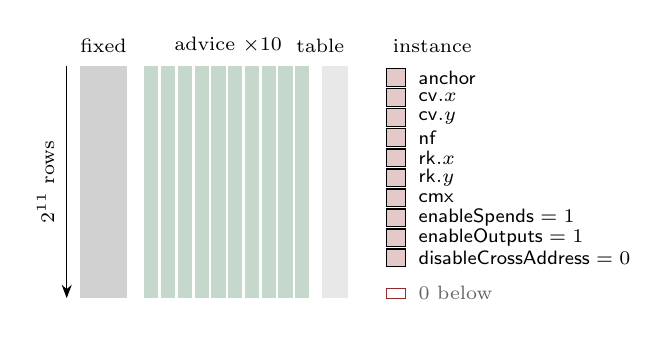
\begin{tikzpicture}[x=0.82cm,y=0.82cm,font=\scriptsize]
  \fill[arbdim!30] (0,0) rectangle ++(0.74,3.6);
  \node[anchor=south] at (0.37,3.65) {fixed};
  \foreach \i in {0,...,9}
    {\fill[arb!25] (1.0+\i*0.26,0) rectangle ++(0.22,3.6);}
  \node[anchor=south] at (2.3,3.65) {advice $\times 10$};
  \fill[arbdim!15] (3.75,0) rectangle ++(0.4,3.6);
  \node[anchor=south east] at (4.25,3.65) {table};
  \foreach \i in {0,...,9}
    {\draw[fill=arbred!25] (4.75,3.28-\i*0.31) rectangle ++(0.3,0.27);}
  \draw[arbred] (4.75,0) rectangle ++(0.3,0.15);
  \node[anchor=south west] at (4.7,3.65) {instance};
  \foreach \i/\l in {0/$\mathsf{anchor}$,1/$\cvsym.x$,2/$\cvsym.y$,
      3/$\nfsym$,4/$\rksym.x$,5/$\rksym.y$,6/$\cmx$,
      7/$\mathsf{enableSpends} = 1$,8/$\mathsf{enableOutputs} = 1$,
      9/$\mathsf{disableCrossAddress} = 0$}
    {\node[anchor=west] at (5.1,3.415-\i*0.31) {\l};}
  \node[anchor=west,text=arbdim] at (5.1,0.075) {$0$ below};
  \draw[-{Stealth}] (-0.2,3.6) -- (-0.2,0)
    node[midway,left=1pt,rotate=90,anchor=south] {$2^{11}$ rows};
\end{tikzpicture}}

\begin{board}{A zk-SNARK, precisely enough}{all four checks}
\Write
\begin{enumerate}
  \item Relation $R$: public statement $x$, private witness $w$.
  \item[] $\mathrm{Prove}(x, w) \to \pi, \qquad
    \mathrm{Verify}(x, \pi) \in \{0, 1\}$
  \item Knowledge sound: an extractor pulls a $w$ with $(x, w) \in R$
    out of any convincing prover.
  \item Zero knowledge: a simulator given only $x$ reproduces $\pi$.
  \item Schnorr $=$ proof of knowledge of $\log_G X$. SNARK $=$ the
    same, for any relation.
\end{enumerate}
\Say
\textbf{In Bitcoin the validator holds everything it checks.} The
witness sits in the transaction; the node re-runs the script and checks
the signature against data in front of it. Here the validator holds
only the public statement $x$ and a short string $\pi$; the witness $w$
never leaves the prover.

\textbf{Knowledge soundness is the property to insist on.} Plain
soundness would allow ``a spendable note exists'' --- other people's
notes exist. The extractor is the point: from any prover that convinces
the verifier, a $w$ with $(x, w) \in R$ can be pulled out, so the
prover must \emph{hold} one.

\textbf{Zero knowledge is the other half.} A simulator given only $x$
reproduces $\pi$: the proof adds nothing beyond the statement. What
that does and does not buy is the next board.

\textbf{The contrast to emphasise.} A Schnorr signature is already a
proof of knowledge, for the one relation ``I know $\log_G X$''. A SNARK
is the same guarantee for any relation --- here the ten clauses of the
Action statement.
\Avoid
``The proof hides the sender and the receiver.'' The proof hides the
witness; whether the published fields can be linked is a separate
question (next board).
\src{\emph{Crypto Guide}, ``SNARKs: succinct non-interactive arguments of
knowledge''; ``Knowledge soundness and extractors''; ``The simulation
paradigm and zero knowledge''}
\end{board}

\begin{board}{Zero knowledge: what $\pi$ hides, and what it does not}
  {all four checks}
\Write
\begin{enumerate}
  \item Whatever a verifier learns from $\pi$, a simulator produces
    from $x$ alone.
  \item Published: $\nfsym$, $\rksym$, $\cvsym$, $\cmx$.
  \item Unlinkable because of: commitment hiding, the keyed nullifier
    PRF, key re-randomisation --- not $\pi$.
  \item Zero knowledge: necessary, not sufficient. A perfect proof
    beside $\nfsym = \cmx$ hides nothing.
\end{enumerate}
\Say
\textbf{The proof reveals nothing beyond the public inputs.} That is
the whole content of zero knowledge: whatever a verifier learns from
$\pi$, a simulator produces from $x$ alone.

\textbf{But the public inputs are published.} The nullifier, the
re-randomised key, the value commitment, the note commitment all go on
chain. That they cannot be linked back to the note and the key rests on
other assumptions --- commitment hiding, the keyed nullifier PRF, key
re-randomisation, from Parts C and E --- not on $\pi$.

\textbf{Zero knowledge is necessary, not sufficient.} Put a perfect
proof beside a nullifier equal to $\cmx$ and it hides nothing.

\textbf{The contrast.} Bitcoin's witness is the secret's public shadow:
a signature, a script preimage. Here the witness never leaves the
prover, and the shadow is the public-input tuple, unlinkable for
reasons the proof does not supply.
\Avoid
``The proof hides the sender and the receiver.'' Unlinkability of the
published tuple is bought by hiding commitments, the keyed PRF and
re-randomisation, not by $\pi$.
\src{\emph{Crypto Guide}, ``The simulation paradigm and zero
knowledge''; \emph{Ironwood Guide}, ``Zero knowledge''}
\end{board}

\begin{board}{Succinct, and non-interactive}{all four checks}
\Write
\begin{enumerate}
  \item Succinct: proof size logarithmic in the circuit ---
    commitments and openings, never the polynomials. One linear MSM,
    shared across a batch.
  \item[] $\text{challenge} := \mathrm{Hash}(\text{everything sent so
    far})$ \quad (Fiat--Shamir)
  \item Proof of knowledge $+$ Fiat--Shamir $=$ signature.
\end{enumerate}
\Say
\textbf{Succinct means the polynomials never travel.} The proof is
logarithmic in the circuit: commitments and openings only. Halo 2's
verifier still pays one linear multi-scalar multiplication, shared
across a batch; it is a SNARK in the proof-size sense.

\textbf{Non-interactive means the coin is a hash.} Wherever a live
verifier would toss a coin, the prover computes the challenge as a hash
of everything sent so far, statement and every commitment included. A
commitment is an input of the hash, so it is fixed before the
challenge that tests it exists. The proof becomes one static object;
verification recomputes the hashes and runs the same checks.

\textbf{The contrast.} A full node that has never met Alice verifies
her Action long after it was made, from the proof string alone.
Schnorr is Fiat--Shamir applied to the log relation: proof of
knowledge plus Fiat--Shamir is a signature; a SNARK is the same recipe,
kept short.
\Avoid
Verification-time figures. The deck says $O(\log n)$ per proof plus one
shared linear MSM, nothing in milliseconds.
\src{\emph{Crypto Guide}, ``SNARKs: succinct non-interactive arguments of
knowledge''; ``The Fiat--Shamir transform: from interactive to
non-interactive''; \emph{Halo 2 Guide}, ``Removing the verifier: the
Fiat--Shamir transform''}
\end{board}

\begin{board}{Arithmetisation: the claim becomes a table}
  {all four checks}
\Draw
Rule eleven columns; brace $a, b, c$ as \emph{advice}, $q_M \dots q_C$
as \emph{fixed}, $\mathrm{PI}$ as \emph{instance}. Write the rows top to
bottom:
\begin{center}\small
\begin{tabular}{@{}c ccc ccccc c l@{}}
\toprule
& \multicolumn{3}{c}{advice} & \multicolumn{5}{c}{fixed} & instance & \\
\cmidrule(lr){2-4}\cmidrule(lr){5-9}\cmidrule(lr){10-10}
row & $a$ & $b$ & $c$ & $q_M$ & $q_L$ & $q_R$ & $q_O$ & $q_C$
  & $\mathrm{PI}$ & gate \\
\midrule
0 & 3 & 3 & 9 & 1 & 0 & 0 & $-1$ & 0 & 0 & $x \cdot x = x^2$ \\
1 & 9 & 3 & 27 & 1 & 0 & 0 & $-1$ & 0 & 0 & $x^2 \cdot x = x^3$ \\
2 & 27 & 3 & 30 & 0 & 1 & 1 & $-1$ & 0 & 0 & $x^3 + x = s$ \\
3 & 30 & 0 & 0 & 0 & 1 & 0 & 0 & 5 & $-35$ & $s + 5 = 35$ \\
\bottomrule
\end{tabular}
\end{center}
\Write
\begin{enumerate}
  \item Toy claim: ``I know $x$ with $x^3 + x + 5 = 35$'' over
    $\F_{97}$ ($x = 3$).
  \item[] $q_M\, a\, b + q_L\, a + q_R\, b + q_O\, c + q_C +
    \mathrm{PI} = 0$ \quad on every row
  \item Copy constraints: $a_0 = b_0 = b_1 = b_2$, $c_0 = a_1$,
    $c_1 = a_2$, $c_2 = a_3$.
  \item Range check $=$ lookup into a table, not algebra.
\end{enumerate}
\Say
\textbf{The Action statement in miniature.} ``I know $x$ with
$x^3 + x + 5 = 35$'' over $\F_{97}$; the answer is $3$. One operation
per row, one gate equation evaluated on every row.

\textbf{Three kinds of column.} Advice is the prover's secret trace.
Fixed columns are the circuit: the selectors pick which operation a row
performs. The instance column carries the public $35$.

\textbf{Wiring and lookups.} Copy constraints wire the rows: the $x$ in
row 0 is the $x$ in rows 1 and 2, and each row's output feeds the next.
A range check is not algebra; it is a lookup into a table.

\textbf{The contrast.} Bitcoin Script is executed by every validator; a
circuit is never executed, only checked.
\Ask
Which column does the verifier never see? --- Advice: the prover's
trace. Fixed columns are the circuit, known to everyone; the instance
column is the public $35$.
\src{\emph{Halo 2 Guide}, ``From computation to a grid of constraints'';
``Proving a value sits in a table: lookups''; ``PLONKish
arithmetisation''}
\end{board}

\begin{board}{Rows become polynomials}{all four checks}
\Write
\begin{enumerate}
  \item Roots of unity in $\F_{97}$: $\omega = 22$, $\omega^2 = 96 =
    -1$, $\omega^4 = 1$; row $i$ lives at $\omega^i \in H = \{1, 22,
    96, 75\}$.
  \item[] $a(1) = 3,\ a(22) = 9,\ a(96) = 27,\ a(75) = 30
    \ \Longrightarrow\ a(X) = 90 + 61X + 22X^2 + 24X^3$
  \item[] $G(X) := q_M a b + q_L a + q_R b + q_O c + q_C + \mathrm{PI},
    \qquad \deg G \le 9$
  \item[] every gate holds $\iff G(\omega^i) = 0$ for all $i$
    $\iff G$ vanishes on $H$
\end{enumerate}
\Say
\textbf{Name the rows by roots of unity.} In $\F_{97}$ the number $22$
is a fourth root of unity, so the four rows live at $1, 22, 96, 75$.

\textbf{Interpolate each column.} The advice column $a$ becomes the
unique polynomial of degree below $4$ through its four values. Four
numbers in, four coefficients out: the column \emph{is} the polynomial,
sampled at the rows. Likewise $b$, $c$ and the public columns.

\textbf{Substitute into the gate.} The polynomial $G$ has degree at most
$9$, and $G(\omega^i)$ is exactly row $i$'s gate equation. So every
gate holds if and only if $G$ vanishes on $H$.

\textbf{The contrast.} A Merkle root also folds many rows into one
object, but it opens one leaf at a time; a polynomial can be probed
anywhere.
\src{\emph{Halo 2 Guide}, ``From the grid to polynomials''}
\end{board}

\begin{board}{All rows at once: one identity, or none}{all four checks}
\Write
\begin{enumerate}
  \item[] $\wbGZH(X) := \prod_{h \in H}(X - h) = X^4 - 1$
  \item[] $G$ vanishes on $H \iff \wbGZH \mid G \iff G = t \cdot
    \wbGZH$
  \item Honest: $\deg G = 9$, $\deg t = 5$, remainder $0$.
  \item Cheat, $c_0 = 10$: row $0$ reads $3 \cdot 3 - 10 = -1 \neq 0$,
    so $\wbGZH \nmid G^{*}$.
  \item[] $D(X) := G^{*}(X) - t^{*}(X)\, \wbGZH(X) =
    24\,(1 + X + X^2 + X^3) \neq 0$
\end{enumerate}
\Say
\textbf{The vanishing polynomial.} The polynomial that is zero exactly
on the rows is $X^4 - 1$. By the factor theorem, applied four times,
$G$ vanishes on $H$ if and only if $\wbGZH$ divides $G$, that is, $G =
t \cdot \wbGZH$ for some quotient $t$.

\textbf{Honest and dishonest traces.} The honest trace divides exactly:
degree $9$ over degree $4$, quotient of degree $5$, remainder zero. Let
the prover claim $x^2 = 10$ and write $c_0 = 10$: row $0$'s gate no
longer holds, $\wbGZH$ no longer divides $G^{*}$, and the Euclidean
division leaves the remainder $24(1 + X + X^2 + X^3)$.

\textbf{The one thing to keep.} A correct computation \emph{is} a
polynomial identity; a wrong one cannot be. The copy constraints get
the same treatment (a running product that equals $1$ when the wiring
holds and, at random challenges, almost never otherwise), and so do
lookups.

\textbf{The contrast.} Bitcoin's validator checks each input's script
on its own; here every row collapses into one identity that holds
everywhere or fails almost everywhere.
\src{\emph{Halo 2 Guide}, ``From vanishing to a single identity'';
``Enforcing the wiring: the permutation argument''}
\end{board}

\begin{board}{One random point: the protocol}{all four checks}
\Write
\begin{enumerate}
  \item Prover commits to $a, b, c$ and $t$; verifier knows $q_M,
    \dots, q_C$ and $\mathrm{PI}$.
  \item Transcript hash draws $z \in \F$ (Fiat--Shamir; BLAKE2b in the
    deployed transcript).
  \item Prover opens $a(z), b(z), c(z), t(z)$ with short proofs.
  \item Verifier forms $G(z)$, computes $\wbGZH(z) = z^4 - 1$, checks
  \item[] $G(z) \overset{?}{=} t(z)\, \wbGZH(z)$
  \item Honest, $z = 20$: $\wbGZH(20) = 46$, $t(20) = 67$, $G(20) = 75
    = 67 \cdot 46$. \checkmark
\end{enumerate}
\Say
\textbf{Four moves.} The prover commits to the advice columns and the
quotient; the fixed and instance columns the verifier already knows.
The transcript hash draws a random point $z$. The prover opens the
committed polynomials at $z$, with short proofs that these are the
committed values. The verifier assembles $G(z)$ from the openings,
computes $z^4 - 1$ itself, and checks one field equation.

\textbf{Run the numbers.} At $z = 20$: $\wbGZH(20) = 46$, $t(20) =
67$, and $G(20) = 75$, which is $67 \cdot 46$ in $\F_{97}$. Every honest
prover passes at every $z$, because $G = t\,\wbGZH$ holds as
polynomials.

\textbf{The contrast.} Bitcoin's validator re-executes the script; this
one evaluates one equation at one point.
\src{\emph{Halo 2 Guide}, ``Why checking one random point is a proof'';
``Removing the verifier: the Fiat--Shamir transform''; ``The complete
Halo 2 protocol''}
\end{board}

\begin{board}{One random point: why a lie is caught}{all four checks}
\Write
\begin{enumerate}
  \item Cheat: $D := G^{*} - t^{*} \wbGZH \neq 0$, frozen before $z$ is
    drawn.
  \item[] $\Pr_{z}[\text{cheat accepted}] = \Pr_z[D(z) = 0] \le
    \dfrac{\deg D}{|\F|}$ \quad (Schwartz--Zippel)
  \item Roots of $D = 24(1 + X + X^2 + X^3)$: $\{22, 75, 96\}$;
    $3/97$ for that $t^{*}$, $9/97$ for any admissible $t^{*}$.
  \item At $z = 20$: $G^{*}(20) = 20$ but $t^{*}(20)\,\wbGZH(20) =
    64$. Caught.
  \item Over $\Fpp$, $\deg D \approx 2^{14}$: about $2^{-240}$; the
    discrete-log layer gives about $126$ bits.
\end{enumerate}
\Say
\textbf{The lie is frozen first.} The commitments pin $G^{*}$ and
$t^{*}$ before $z$ is drawn, so the difference $D$ is a fixed nonzero
polynomial. The check passes exactly when $D(z) = 0$, and a nonzero
polynomial has at most $\deg D$ roots --- Schwartz--Zippel.

\textbf{On the toy.} For the $c_0 = 10$ cheat the roots are $22$, $75$
and $96$: the three rows where the tampered gate still held. That is
$3/97$ for this quotient, $9/97$ for any admissible one. At $z = 20$
the two sides read $20$ and $64$: caught.

\textbf{At scale.} Over $\Fpp$ with $\deg D$ around $2^{14}$ the term is
about $2^{-240}$. That is one Schwartz--Zippel term, not the system's
security level; the discrete-log layer gives about $126$ bits.

\textbf{The one thing to keep.} A false statement is too rigid to hide:
it disagrees with the truth almost everywhere, and one probe lands
where it disagrees. Bitcoin never needs this; its validator sees the
data.
\Ask
Why $3/97$ for this cheat but $9/97$ in general? --- This $D$ has
exactly three roots, the rows where the tampered gate still held; the
general bound is $\deg D \le 9$.
\Avoid
Quoting $2^{-240}$ as the security level. It is one Schwartz--Zippel
term; the system rests on discrete log at about $126$ bits.
\src{\emph{Halo 2 Guide}, ``Why checking one random point is a proof'';
\emph{Math Guide}, ``The Schwartz--Zippel lemma''}
\end{board}

\begin{board}{Committing to a polynomial: the problem}{all four checks}
\Write
\begin{enumerate}
  \item Needed: a short commitment $P$ to $f$, and a short proof that
    $f(x) = v$ at a drawn $x$ for the committed $f$.
  \item[] $P = \Comm(f; r) = \ip{\vec a}{\vec G} + [r]\,H \in \G$
  \item One Vesta point for $2^{11}$ coefficients. Binding under
    discrete log; hiding by $[r]H$; no secret behind $\vec G$.
  \item Merkle: one entry in $\log_2 d$ hashes. IPA: a combination of
    all entries in $2\log_2 d$ points.
\end{enumerate}
\Say
\textbf{The random point needs the polynomials fixed first.} The
argument on the last two boards assumed the polynomials were pinned
before $z$ was drawn. So we need a short commitment to $f$, and a short
proof that $f(x) = v$ at a drawn point for the committed $f$.

\textbf{Pedersen, vectorised.} Commit to the coefficient vector with
generators $\vec G$ and $H$ hashed into existence: one Vesta point
stands for $2^{11}$ coefficients. Binding under discrete log, hiding by
the $[r]H$ term, and no secret behind $\vec G$.

\textbf{The contrast.} A Merkle root also commits to a vector, and
opens one entry in $\log_2 d$ hashes; the next board opens a linear
combination of \emph{all} entries in $2\log_2 d$ points.
\src{\emph{Halo 2 Guide}, ``Why the prover cannot wriggle: binding
commitments''; \emph{Crypto Guide}, ``Polynomial commitment schemes'';
``Hashing to a curve point''}
\end{board}

\begin{board}{Committing to a polynomial: the opening claim}
  {all four checks}
\Write
\begin{enumerate}
  \item[] $f(x) = \ip{\vec a}{\vec b(x)}, \qquad \vec b(x) := (1, x,
    x^2, \dots, x^{d-1})$
  \item[] $P + [v]\,U = \ip{\vec a}{\vec G} + [r]\,H +
    [\ip{\vec a}{\vec b}]\,U$
  \item Sending $\vec a$: $d$ elements. Inner-product argument:
    $2\log_2 d$ points, $22$ for $d = 2^{11}$.
\end{enumerate}
\Say
\textbf{Evaluation is an inner product.} The value $f(x)$ is the
coefficient vector dotted with the public vector of powers of $x$.

\textbf{Fold the claimed value into the commitment.} With a second
hashed generator $U$, the opening claim becomes one group equation:
$P + [v]U$ equals the commitment plus the inner product times $U$.

\textbf{The cost.} Sending $\vec a$ would cost $d$ elements. The
inner-product argument --- the Bulletproofs family you know from range
proofs --- proves the inner product in $2\log_2 d$ points: $22$ for
$d = 2^{11}$.

\textbf{The contrast.} A Merkle proof names one leaf; an IPA opening is
one number computed from every coefficient, at a point chosen after
they were fixed.
\Ask
How many points does the opening cost for $d = 2^{11}$? ---
$2 \log_2 d = 22$.
\src{\emph{Halo 2 Guide}, ``The inner-product polynomial commitment'';
\emph{Crypto Guide}, ``Polynomial commitment schemes''}
\end{board}

\begin{board}{The inner-product argument: one fold}{all four checks}
\Write
\begin{enumerate}
  \item Split: $\vec a = (\wbGlo{\vec a}, \wbGhi{\vec a})$, likewise
    $\vec G$ and $\vec b$.
  \item[] $L := \ip{\wbGlo{\vec a}}{\wbGhi{\vec G}} + [\ell]\,H
      + [\ip{\wbGlo{\vec a}}{\wbGhi{\vec b}}]\,U$
  \item[] $R := \ip{\wbGhi{\vec a}}{\wbGlo{\vec G}} + [r_R]\,H
      + [\ip{\wbGhi{\vec a}}{\wbGlo{\vec b}}]\,U$
  \item Challenge $u$; fold:
  \item[] $\vec a' := u\,\wbGlo{\vec a} + u^{-1}\wbGhi{\vec a}, \quad
    \vec G' := u^{-1}\wbGlo{\vec G} + u\,\wbGhi{\vec G}, \quad
    \vec b' := u^{-1}\wbGlo{\vec b} + u\,\wbGhi{\vec b}$
  \item[] $\ip{\vec a'}{\vec G'} = \ip{\vec a}{\vec G} +
    u^2 \ip{\wbGlo{\vec a}}{\wbGhi{\vec G}} +
    u^{-2} \ip{\wbGhi{\vec a}}{\wbGlo{\vec G}}$
  \item[] $P + [v]\,U + [u^2]\,L + [u^{-2}]\,R
    = \ip{\vec a'}{\vec G'} + [r + u^2 \ell + u^{-2} r_R]\,H
    + [\ip{\vec a'}{\vec b'}]\,U$
\end{enumerate}
\Say
\textbf{Halve everything.} Split each vector into a low and a high
half and publish the two cross terms $L$ and $R$: low $\vec a$ against
high $\vec G$ and $\vec b$, and the reverse, each with its own blinder.

\textbf{Fold with a challenge.} Draw $u$ and fold, both parties in
step: the prover folds $\vec a$ with weights $(u, u^{-1})$, the
verifier folds $\vec G$ and $\vec b$ with the inverse weights.

\textbf{Multiply out.} The folded inner product is the old one plus
$u^2$ times one cross term plus $u^{-2}$ times the other, and the same
for $\vec b$. So the old claim plus $[u^2]L + [u^{-2}]R$ is the same
claim at half the length. The verifier updates $\vec G'$ and $\vec b'$
by public arithmetic and never sees $\vec a$.

\textbf{The contrast.} This is the textbook (Bulletproofs) form; a
Bulletproofs range proof folds its vectors by exactly this move.
\Avoid
Presenting $[u^2]L + [u^{-2}]R$ as the deployed accumulation; it is the
textbook form. The deployed rescaling comes two boards on.
\src{\emph{Halo 2 Guide}, ``The inner-product polynomial commitment'',
Construction ``IPA-based polynomial commitment''}
\end{board}

\begin{board}{The inner-product argument: the recursion}
  {all four checks}
\Write
\begin{enumerate}
  \item After $k = \log_2 d$ rounds every vector has length $1$.
  \item Proof: $2k$ points $(L_j, R_j)$, final scalar $a$, blinder
    $r^{*} = r + \sum_j (u_j^2 \ell_j + u_j^{-2} r_j)$.
  \item[] $P + [v]\,U + \sum_{j=1}^{k}\bigl([u_j^2]\,L_j +
    [u_j^{-2}]\,R_j\bigr) \overset{?}{=} [a]\,G^{(0)} + [r^{*}]\,H +
    [a \cdot b^{(0)}]\,U$
  \item[] $b^{(0)} = \prod_{\ell}(u_\ell^{-1} + u_\ell\,
    x^{2^{\ell-1}})$ \quad $O(\log d)$ field operations
  \item[] $G^{(0)} = \ip{\vec s}{\vec G}$ \quad an MSM of length $d$
\end{enumerate}
\Say
\textbf{Fold until one element remains.} After $\log_2 d$ rounds every
vector has length one. The proof is the $2k$ cross terms, the final
scalar $a$, and the aggregated blinder. The verifier accumulates the
cross terms into the commitment and checks one group equation.

\textbf{Two verifier costs.} The scalar $b^{(0)}$ is a product of
$\log d$ factors --- cheap. The point $G^{(0)}$ is a multi-scalar
multiplication of length $d$ --- the one linear step. The node shares
it across a batch; recursion would defer it into an accumulator, which
is not deployed.

\textbf{Why it binds.} Two openings of one commitment would exhibit a
non-trivial discrete-log relation among $\vec G, H$ on Vesta; an
extractor rewinds three challenges per round.

\textbf{The contrast.} A Bitcoin signature check costs a fixed handful
of group operations; an IPA opening is logarithmic in size but ends in
a circuit-sized wall of group arithmetic.
\Avoid
Claiming recursion or accumulation is deployed. The node verifies each
proof directly and shares the MSM across a batch.
\src{\emph{Halo 2 Guide}, ``The inner-product polynomial commitment'';
``Accumulation and the Halo trick''; \emph{Crypto Guide}, ``Polynomial
commitment schemes''}
\end{board}

\begin{board}{What the fold hides, and the deployed normalisation}
  {all four checks}
\Write
\begin{enumerate}
  \item Folding alone is not zero knowledge: the final $a$ is a
    challenge-dependent linear form in the coefficients.
  \item Deployed: mask $f$ by a random polynomial vanishing at the
    opening point, commit as $S$, draw two more challenges, then fold.
  \item Deployed weights: $(1, u_j^{-1})$ on coefficients, $(1, u_j)$
    on $\vec b$ and $\vec G$; accumulate $[u_j^{-1}]\,L_j + [u_j]\,R_j$.
  \item Same $2k$ points, plus $S$ and two final scalars.
\end{enumerate}
\Say
\textbf{Folding alone leaks.} The final scalar $a$ is a linear form in
the coefficients whose weights the challenges fix; blinding $P$ and the
round points hides those points, not $a$.

\textbf{The deployed fix.} The opening first masks $f$ by a random
polynomial vanishing at the opening point, commits to the mask as $S$,
draws two further challenges, and only then folds.

\textbf{The deployed rescaling.} The fold weights are $(1, u_j^{-1})$
on the coefficients and $(1, u_j)$ on $\vec b$ and $\vec G$, and the
verifier accumulates $[u_j^{-1}]L_j + [u_j]R_j$. The two conventions
are related by per-round rescaling; the previous board's form is the
textbook one, and the deployed proof carries the same $2k$ points plus
$S$ and two final scalars.

\textbf{The contrast.} A Bitcoin signature exposes its public key by
design; here even the last scalar of an opening must be masked.
\src{\emph{Halo 2 Guide}, ``The inner-product polynomial commitment'',
Remarks ``Folding alone is not zero knowledge'', ``The deployed IPA
normalisation''}
\end{board}

\begin{board}{The fold by hand: two rounds}{all four checks}
\Draw
Write the setup line first, then the table, one round per row:
\begin{center}\small
\begin{tabular}{@{}l ccc ccc c@{}}
\toprule
round & $L_j$ & $R_j$ & $u_j$ & $\vec a'$ & $\vec b'$ & $\vec G'$
  & fold check \\
\midrule
$j = 2$ ($\ell_2, r_2 = 19, 23$) & $13$ & $4$ & $3$ & $(15, 68)$
  & $(92, 82)$ & $(48, 22)$ & $25 = 25$ \\
$j = 1$ ($\ell_1, r_1 = 29, 31$) & $52$ & $58$ & $5$ & $(11)$ & $(21)$
  & $(42)$ & $12 = 12$ \\
\bottomrule
\end{tabular}
\end{center}
\Write
\begin{enumerate}
  \item Toy: $p(X) = 5 + X + X^3$ opened at $x = 3$, so $v = 35$.
    Group: $\mathbb{Z}_{97}$ written additively, $[k]G = kG \bmod 97$.
  \item[] $\vec a = (5, 1, 0, 1), \quad \vec b = (1, 3, 9, 27), \quad
    \vec G = (2, 3, 5, 7)$
  \item[] $H = 11, \quad U = 13, \quad r = 17, \qquad
    P = \ip{\vec a}{\vec G} + [r]H = 13$
  \item Fold check per row: $\ip{\vec a'}{\vec G'} + [r^{*}]H +
    [\ip{\vec a'}{\vec b'}]U = P + [v]U + [u^2]L + [u^{-2}]R$.
\end{enumerate}
\Say
\textbf{The Halo 2 Guide's symbolic example, with numbers.} The toy
polynomial $5 + X + X^3$ is opened at $x = 3$, so the claimed value is
$35$. The stand-in group is $\mathbb{Z}_{97}$ written additively: a
``point'' is a residue and a scalar multiple is a product mod $97$. It
has no discrete-log hardness, only the fold's algebra.

\textbf{Round two, then round one.} With four coefficients there are
two rounds. Each row shows the cross terms, the challenge, the three
folded vectors, and the fold check: the folded claim on the left equals
the accumulated commitment on the right --- $25 = 25$, then $12 = 12$.

\textbf{The one thing to keep.} Each row's check is exactly the
one-fold identity from three boards back, instantiated.
\Avoid
Calling $\mathbb{Z}_{97}$ a curve, or claiming the toy is binding or
hiding. Anyone can divide in $\mathbb{Z}_{97}$; the numbers show only
the algebra.
\src{\emph{Halo 2 Guide}, ``The inner-product polynomial commitment''}
\end{board}

\begin{board}{The fold by hand: the final check}{all four checks}
\Write
\begin{enumerate}
  \item Prover sends $a = 11$ and $r^{*} = 30$.
  \item[] $\vec s = (u_1^{-1}u_2^{-1},\ u_1 u_2^{-1},\ u_1^{-1}u_2,\
    u_1 u_2) = (13, 34, 20, 15), \qquad G^{(0)} = \ip{\vec s}{\vec G}
    = 42$
  \item[] $b^{(0)} = g(x; u_1, u_2) = (u_1^{-1} + u_1 x)(u_2^{-1} + u_2
    x^2) = 21$
  \item[] $P + [v]U + [u_1^2]L_1 + [u_1^{-2}]R_1 + [u_2^2]L_2 +
    [u_2^{-2}]R_2 = 12$
  \item[] $[a]\,G^{(0)} + [r^{*}]\,H + [a \cdot b^{(0)}]\,U = 12$
\end{enumerate}
\Say
\textbf{The verifier works from the challenges alone.} It builds the
weight vector $\vec s$ from products of the challenges and their
inverses, takes the inner product with $\vec G$ to get $G^{(0)} = 42$,
and evaluates the folded $b$ polynomial to get $b^{(0)} = 21$.

\textbf{Compare the two sides.} The accumulated commitment comes to
$12$; the prover's claimed side comes to $12$. Equal: accepted.

\textbf{What travelled.} Four coefficients were never sent; four points
and two scalars were.

\textbf{The contrast, and the caveat.} In $\mathbb{Z}_{97}$ anyone can
divide, so nothing here is hidden or binding; on Vesta the same
equations are, and $G^{(0)}$ is a length-$2^{11}$ multi-scalar
multiplication.
\src{\emph{Halo 2 Guide}, ``The inner-product polynomial commitment''}
\end{board}

\begin{board}{Fields and curves in the deployed circuit}
  {all four checks}
\Write
\begin{enumerate}
  \item Native field: $\Fpp$, the \emph{base} field of Pallas.
  \item Native points: $\cmsym$, $\rksym$, $\cvsym$, $\aksym$, $\pkd$
    --- coordinates in $\Fpp$, group law by native arithmetic.
  \item Column polynomials committed on Vesta, whose \emph{scalar}
    field is exactly $\Fpp$.
\end{enumerate}
\Say
\textbf{The circuit computes in Pallas's base field.} The points the
statement handles --- the note commitment, the re-randomised key, the
value commitment, the spend key, the diversified key --- have
coordinates there, so the group law is native arithmetic, not emulated.

\textbf{The commitments live on the other curve.} The column
polynomials are committed on Vesta, whose scalar field is exactly
$\Fpp$: the coefficients are the circuit's own field elements.

\textbf{The contrast.} Bitcoin's secp256k1 is one curve doing one job:
its validator verifies signatures, never circuits. And its base field,
as the two-adicity board shows, cannot even host the prover's
evaluation domain.
\src{\emph{Ironwood Guide}, ``Flags, public inputs, and circuit
parameters''; \emph{Math Guide}, ``Base fields, scalar fields, and the
Pasta cycle''}
\end{board}

\begin{board}{The Pasta cycle, once}{all four checks}
\Write
\begin{enumerate}
  \item Pallas over $\Fpp$ has order $p_{\Vesta}$; Vesta over $\Fpv$
    has order $p_{\Pallas}$.
  \item Vesta-committed proof: Vesta points, coordinates in $\Fpv$
    $\to$ verified natively by a circuit over $\Fpv$, committed on
    Pallas.
  \item Its proof: Pallas points, coordinates in $\Fpp$ $\to$ verified
    natively by a circuit over $\Fpp$, committed on Vesta.
  \item Not deployed: the node verifies each bundle's proof directly
    and batches the deferred MSMs.
\end{enumerate}
\Say
\textbf{Each curve's scalar field is the other's base field.} That is
the whole definition of the cycle.

\textbf{Why that lets a verifier be a circuit.} A Vesta-committed proof
is Vesta points with coordinates in Vesta's base field, which is
Pallas's scalar field; the circuit that verifies it natively is one
over that field, committed on Pallas. That circuit's proof is Pallas
points with coordinates in $\Fpp$, verified natively by a circuit over
$\Fpp$, committed on Vesta. Proofs alternate between the two curves,
each verifier a circuit, so one proof can attest to the previous one.

\textbf{Not deployed.} The node verifies each bundle's proof directly
and batches the deferred multi-scalar multiplications.

\textbf{The contrast.} Bitcoin needs no such pair; a signature is
verified by arithmetic, not by another proof.
\Avoid
Presenting recursion as deployed. Say the cycle once, then say
``batched''.
\src{\emph{Halo 2 Guide}, ``A cycle of curves for efficient native
recursion''; ``Accumulation and the Halo trick''; \emph{Math Guide},
``Base fields, scalar fields, and the Pasta cycle''}
\end{board}

\begin{board}{Why not Bitcoin's curve: two-adicity}{all four checks}
\Draw
Write the table, one field per row:
\begin{center}\small
\begin{tabular}{@{}lccc@{}}
\toprule
field & bits & two-adicity of $p - 1$ & largest domain \\
\midrule
$\Fpp$ (Pallas base) & $255$ & $32$ & $2^{32}$ \\
$\Fpv$ (Vesta base) & $255$ & $32$ & $2^{32}$ \\
secp256k1 base field & $256$ & $1$ & $2$ \\
secp256k1 scalar field & $256$ & $6$ & $64$ \\
\bottomrule
\end{tabular}
\end{center}
\Write
\begin{enumerate}
  \item Interpolating over $n = 2^{11}$ rows needs a primitive
    $2^{11}$-th root of unity: $2^{11} \mid p - 1$.
  \item Quotient FFTs run on $8n = 2^{14}$ points at the deployed gate
    degree.
  \item Two-adicity: the largest $k$ with $2^k \mid p - 1$.
  \item Bitcoin's prime $p = 2^{256} - 2^{32} - 977$: $p - 1$ is twice
    an odd number, a domain of two points.
\end{enumerate}
\Say
\textbf{Interpolation needs roots of unity.} Naming $2^{11}$ rows by
roots of unity needs a primitive $2^{11}$-th root, so $2^{11}$ must
divide $p - 1$; the prover's quotient FFTs run on $2^{14}$ points. The
largest power of two dividing $p - 1$ is the field's two-adicity.

\textbf{The Pasta primes were designed for this.} Two-adicity exactly
$32$ in both, so domains of every size up to $2^{32}$.

\textbf{Bitcoin's prime was not.} The secp256k1 curve buys its
implementation speed from $a = 0$; its prime $2^{256} - 2^{32} - 977$
was not chosen for evaluation domains: $p - 1$ is twice an odd number,
so the largest domain has two points. The scalar field manages $64$.

\textbf{Attribution.} The Pasta two-adicity is the Math Guide's, the
prime values the protocol specification's (``Pallas and Vesta''); the
secp256k1 rows are our own computation, not a volume figure.
\Ask
Could secp256k1's base field host even the four-row toy? --- No:
two-adicity $1$, largest domain two points.
\src{\emph{Math Guide}, ``Pallas and Vesta assembled'', Remark
``Two-adicity and FFT-friendly primes''; \emph{Crypto Guide}, ``The
transparent layer's schemes: ECDSA and BIP-340 over secp256k1'';
\emph{Halo 2 Guide}, ``The complete Halo 2 protocol''}
\end{board}

\begin{board}{Trust: what a ceremony is, and why there is none}
  {conserved}
\Write
\begin{enumerate}
  \item[] $pp = \bigl([\tau^0]G, [\tau^1]G, \dots, [\tau^d]G,
    \dots\bigr), \qquad \tau \text{ destroyed}$
  \item Whoever keeps $\tau$ forges: for any $C$, $z$, $y$,
  \item[] $\pi := [(\tau - z)^{-1}]\,(C - [y]G)$ \quad passes, no
    polynomial behind it --- the toxic waste.
  \item Groth16: secrets per circuit. MPC: safe if \emph{one}
    participant destroyed their share. The Sapling pool still rests on
    that.
  \item Bound (ZIP-209): each pool's chain value balance is public and
    may not go negative $\Rightarrow$ counterfeit capped at the pool's
    exit.
  \item Orchard, Ironwood: IPA generators hashed from a public domain
    tag; nothing to leak, nothing to destroy.
\end{enumerate}
\Say
\textbf{Pairing SNARKs bake a secret into the parameters.} The
pairing-based commitment (KZG) shows the shape: the parameters are
powers of a secret $\tau$ in the group, and $\tau$ must be destroyed.
Whoever keeps it forges an opening for any commitment, point and value
--- with no polynomial behind it. That is the toxic waste. Groth16's
secrets are per circuit.

\textbf{The ceremony, and what still rests on it.} A multiparty
ceremony keeps the waste unknown provided one participant destroyed
their share. The Sapling pool still rests on that assumption.

\textbf{The bound.} Under ZIP-209 each pool's chain value balance is
public and may not go negative, so a forged Sapling proof creates value
only inside the Sapling pool and can withdraw at most what that pool
publicly holds --- the turnstile, Part H.

\textbf{Orchard and Ironwood.} The IPA generators are hashed from a
public domain tag: nothing to leak, nothing to destroy; binding rests
on discrete log alone. Bitcoin never had a setup; Sapling has one;
Orchard returns to none.
\Avoid
``No ceremony'' without the Sapling caveat: the Sapling pool still
rests on its MPC. ``The pool is auditable'': the balance is public, but
counterfeit inside the pool is undetectable; the bound acts at the
exit.
\src{\emph{Crypto Guide}, ``Polynomial commitment schemes''; ``SNARKs:
succinct non-interactive arguments of knowledge''; \emph{Halo 2 Guide},
``The ``Halo'' in Halo 2: deferring the expensive check'';
\emph{Ironwood Guide}, ``Pool balances: ZIP-209 and its Ironwood
analogue''}
\end{board}

\begin{board}{Three generations}{all four checks}
\Draw
Three columns, Sprout, Sapling, Orchard and Ironwood; write the rows
top to bottom:
\begin{center}\small
\begin{tabular}{@{}llll@{}}
\toprule
& Sprout & Sapling & Orchard, Ironwood \\
\midrule
SNARK & BCTV14 (original) & Groth16 & Halo 2 \\
curve & BN254 & BLS12-381, Jubjub in-circuit & Pallas, Vesta \\
setup & six-party MPC & large MPC & none \\
hash in circuit & SHA-256 & Pedersen & Sinsemilla \\
proof & 296 B & 192 B & $2720 + 2272a$ B \\
verification & constant & three pairings & $O(\log n)$ + shared MSM \\
\bottomrule
\end{tabular}
\end{center}
\Write
\begin{enumerate}
  \item Sprout: BCTV14 soundness flaw found after deployment; re-proved
    with Groth16, deprecated.
  \item Sapling: Groth16 over BLS12-381, Jubjub inside the circuit.
  \item Orchard: proof grows because transparency costs $2\log_2 n$
    points.
\end{enumerate}
\Say
\textbf{Sprout.} A soundness flaw in BCTV14, found after deployment,
would have allowed undetected counterfeiting; Sprout was re-proved with
Groth16 and deprecated.

\textbf{Sapling.} Groth16 over BLS12-381, Jubjub inside the circuit: a
far faster prover, a per-circuit ceremony, no curve cycle.

\textbf{Orchard and Ironwood.} Halo 2 on Pallas and Vesta, no setup.
The proof grew because transparency costs $2\log_2 n$ points.

\textbf{The contrast.} Bitcoin changed its signature scheme once, by
opt-in; Zcash has carried shielded payments through three proof
systems, each with its own pool --- the third with two, Orchard and
Ironwood, on one circuit.
\Avoid
Years. ``A few hundred bytes'': the sizes are $296$ B, $192$ B, and
$2720 + 2272a$ B, with units. ``No ceremony'' as a blanket statement:
Sapling's still stands.
\src{\emph{Ironwood Guide}, ``Lineage: three generations of shielded
proof''; ``Comparative summary''}
\end{board}

\begin{board}{The Orchard circuit by the numbers}{all four checks}
\Draw
Two columns, label then value; write the rows top to bottom:
\begin{center}\small
\begin{tabular}{@{}ll@{}}
\toprule
rows & $2^{11} = 2048$; one fixed circuit, every Action an instance \\
columns & ten advice, fixed columns, a Sinsemilla lookup table \\
proof per bundle & $2720 + 2272\,a$ B: $4992$ for one Action, $7264$
  for Alice's two \\
of which IPA & $22$ pair points and one blinding commitment, $32$ B
  each \\
proving & a few seconds on commodity hardware \\
verifying & $O(\log n)$ per proof, plus one MSM shared across a batch \\
\bottomrule
\end{tabular}
\end{center}
\Write
\begin{enumerate}
  \item One aggregate proof per bundle: per-Action term $=$ that
    Action's column commitments and evaluations; constant term $=$ the
    shared quotient, multipoint and IPA data.
  \item Spend-auth signature: $64$ B. One-Action proof: $78$
    signatures' worth.
\end{enumerate}
\Say
\textbf{One circuit, one proof per bundle.} The circuit has $2^{11}$
rows and ten advice columns; every Action is an instance of it. One
aggregate proof covers all of a bundle's Actions: the per-Action term
is that Action's column commitments and evaluations, the constant term
the shared quotient, multipoint and IPA data --- $4992$ bytes for one
Action, $7264$ for Alice's two.

\textbf{Where the bytes go.} Of the constant term, the IPA is $22$
pair points and one blinding commitment at $32$ bytes each. A
spend-auth signature is $64$ bytes; a one-Action proof is $78$
signatures' worth.

\textbf{Costs.} Proving takes a few seconds on commodity hardware;
verifying is logarithmic per proof plus one MSM shared across a batch.

\textbf{The contrast.} Bitcoin's witness cost is per input and grows
with the script it satisfies; here it is per bundle, logarithmic in the
circuit, and independent of the anonymity set.
\Avoid
``A few hundred bytes'': it is $4992$ B for one Action. Millisecond
verification figures: the deck states only $O(\log n)$ plus the shared
MSM. ``A few seconds'' is the only timing phrase.
\src{\emph{Ironwood Guide}, ``Flags, public inputs, and circuit
parameters''; ``The v6 transaction and the Ironwood component'';
\emph{Halo 2 Guide}, ``The complete Halo 2 protocol''}
\end{board}

\begin{board}{Five gadget families, three circuit versions}
  {all four checks}
\Write
\begin{enumerate}
  \item ECC: $\rksym = \aksym + [\alpha]\,G^{\mathsf{SpendAuth}}$ (A6),
    $\pkd = [\ivk]\,\gd$ (A7), $\cvsym$ (A4), the nullifier's point
    (A5).
  \item Sinsemilla: generator table as a lookup; per $10$-bit chunk one
    lookup and two incomplete additions; $\NoteCommit$ (A1, A2),
    $\CommitIvk$ (A7).
  \item Merkle path: $32$ layer-tagged hashes, a conditional swap per
    layer by one bit of the position, root $=$ anchor gated by
    $v_{\mathrm{old}}$ (A3).
  \item Poseidon: the nullifier PRF; only non-linearity $x \mapsto x^5$
    (A5).
  \item Decomposition: $v \in [0, 2^{64})$ and the sign bit (A4);
    canonicity of witnessed encodings.
  \item Three versions: original, a correction, the Ironwood circuit
    with the cross-address input. Verifying key selected by branch.
\end{enumerate}
\Say
\textbf{Five families carry the ten clauses.} The Pallas group law
does the key re-randomisation, the diversified key, the value
commitment and the nullifier's point. Sinsemilla, with its generator
table as a lookup, carries both note commitments and the ivk
commitment. The Merkle gadget walks $32$ layer-tagged hashes with a
conditional swap per layer, root equal to the anchor, gated by
$v_{\mathrm{old}}$. Poseidon is the nullifier PRF, its only
non-linearity $x \mapsto x^5$. Decomposition does the $64$-bit range
check, the sign bit, and canonicity of witnessed encodings --- distinct
from the node's parsing of public encodings, Part E.

\textbf{Three versions, one key per branch.} The original circuit, a
correction, and the Ironwood circuit with the cross-address input;
consensus selects the verifying key by branch, so every Action in
either pool now verifies against the Ironwood key.

\textbf{The contrast.} Bitcoin's validator runs whatever script an
output declares; this one runs a verifier keyed to one fixed circuit.
\Avoid
Multiplicative re-randomisation: it is $\aksym + [\alpha]\,G$, never
$[\alpha]\,\aksym$. The position as $\rho$: the position is a private
witness of the Merkle gadget and never enters the nullifier.
\src{\emph{Ironwood Guide}, ``The gadget set''; ``One circuit, one
verifying key''}
\end{board}

\begin{board}{Alice's Action as an instance}{all four checks}
\Draw
\begin{enumerate}
  \item A tall grid: one grey column at the left, labelled
    \emph{fixed}; ten thin green columns, labelled \emph{advice}
    $\times 10$; a light grey column, labelled \emph{table}.
  \item A vertical arrow down the left edge, labelled $2^{11}$ rows.
  \item To the right, one narrow column of ten red cells, labelled
    \emph{instance}, with one small empty cell at the bottom marked
    ``$0$ below''.
  \item Label the ten cells top to bottom: $\mathsf{anchor}$,
    $\cvsym.x$, $\cvsym.y$, $\nfsym$, $\rksym.x$, $\rksym.y$, $\cmx$,
    $\mathsf{enableSpends} = 1$, $\mathsf{enableOutputs} = 1$,
    $\mathsf{disableCrossAddress} = 0$.
\end{enumerate}
\begin{center}
\wbGInstanceFig
\end{center}
\Write
\begin{enumerate}
  \item Instance (Action 1: $2$ ZEC $\to$ Bob $1.5$): eight public
    inputs, ten field elements; points by coordinates; flags as the
    Ironwood component sets them.
  \item Advice: both notes; $32$ siblings and the position; $\aksym$,
    $\nksym$, $\rivk$, $\ivk$; $\alpha$; $\rcv$;
    $(\mathrm{magnitude}, \mathrm{sign}) = (50\,000\,000, +1)$.
  \item Copy constraints tie each instance cell to the advice cell
    holding the same value.
\end{enumerate}
\Say
\textbf{The public column, for Alice's first Action.} Eight named
public inputs make ten field elements: the two points enter by their
coordinates, and the three flags as the Ironwood component sets them.
Below the tenth cell the column is zero.

\textbf{The advice cells hold everything secret.} Both notes, the
$32$ siblings and the position, the keys $\aksym$, $\nksym$, $\rivk$,
$\ivk$, the re-randomiser $\alpha$, the value-commitment trapdoor
$\rcv$, and the value as magnitude and sign: $50\,000\,000$ and $+1$.

\textbf{How the public column binds.} Copy constraints tie each
instance cell to the advice cell holding the same value; the verifier
computes the instance commitment itself, so a proof for other values
fails the opening.

\textbf{The contrast.} Bitcoin's witness --- scriptSig or witness field
--- is in the clear; here the witness fills advice cells nobody reads.
\Ask
Checkpoint: what could a holder of the Sapling ceremony's toxic waste
do, what stops the analogue in Orchard, and what bounds the damage?
\begin{itemize}
  \item Forge accepting Sapling proofs of false statements: counterfeit
    inside the Sapling pool, invisible to every verifier. Not decrypt
    notes --- soundness and zero knowledge are separate guarantees.
  \item In Orchard there is no trapdoor to hold: the generators are
    hashed, and binding reduces to discrete log.
  \item Under ZIP-209 each pool's chain value balance is public, and a
    block that would drive it negative is invalid --- counterfeit is
    capped at the pool's exit.
\end{itemize}
\Avoid
``The proof hides sender and receiver'': the instance tuple is public
and unlinkable for reasons outside $\pi$. Answering the checkpoint with
``decrypt notes'': toxic waste breaks soundness, not zero knowledge.
``The pool is auditable'': the bound acts at the exit, not inside.
\src{\emph{Ironwood Guide}, ``The Action statement, formally'';
\emph{Halo 2 Guide}, ``Instance columns and binding the public
statement''; checkpoint: \emph{Crypto Guide}, ``SNARKs: succinct
non-interactive arguments of knowledge''; \emph{Ironwood Guide}, ``Pool
balances: ZIP-209 and its Ironwood analogue''}
\end{board}

%% ---- 08-delivery.tex
%% Part F --- Delivery and light clients (whiteboard companion)
%% Drafted from the verified deck fragment draft/08-delivery.tex.
%% Numbers: compute/f_delivery.py, compute/f_lightclient.py, compute/f_rcm.py.

\newcommand{\wbFenc}{\ensuremath{C_{\mathrm{enc}}}}
\newcommand{\wbFout}{\ensuremath{C_{\mathrm{out}}}}
\newcommand{\wbFnp}{\ensuremath{\mathsf{np}}}
\newcommand{\wbFrseed}{\ensuremath{\mathsf{rseed}}}
\newcommand{\wbFock}{\ensuremath{\mathsf{ock}}}
\newcommand{\wbFpre}{\ensuremath{\mathsf{pre}_{\rcm}}}
\newcommand{\wbFivkint}{\ensuremath{\ivk^{\mathsf{int}}}}
\newcommand{\wbFkenc}{\ensuremath{K_{\mathrm{enc}}}}

\section{Part F --- Delivery and light clients}

\begin{board}{The note plaintext: what travels to Bob}{exists}
\Write
\begin{enumerate}
  \item $\wbFnp := (\mathtt{0x03},\ d,\ v,\ \wbFrseed,\ \mathsf{memo})$
  \item $1 + 11 + 8 + 32 + 512 = 564$ bytes
  \item $\wbFrseed \to \esk$ \quad
    ($\mathsf{PRFexpand}_{\wbFrseed}(\mathtt{0x04} \,\|\, \rho)$)
  \item $\wbFrseed \to \psi$ \quad
    ($\mathsf{PRFexpand}_{\wbFrseed}(\mathtt{0x09} \,\|\, \rho)$)
  \item $\wbFrseed \to \rcm$ \quad (next board)
  \item $\rho := \nfsym_{\mathrm{old}}$
\end{enumerate}
\Say
\textbf{The chain stores only \cmx; the note itself must still reach
Bob.} In Bitcoin the output is the note: amount and script sit on chain
and the recipient's wallet reads them there. Here the chain holds a
commitment, so Alice has to deliver the opening herself. What she sends
is the note plaintext.

\textbf{The lead byte names the format.} Byte $\mathtt{0x03}$ is the
Ironwood note, the only value the Ironwood pool admits.

\textbf{The 32-byte seed is the note's whole randomness.} Three
$\mathsf{PRFexpand}$ calls keyed by \wbFrseed, each under its own domain
byte, yield \esk, $\psi$ and \rcm{} (next board); with $\rho :=
\nfsym_{\mathrm{old}}$ the seed is bound to its Action.

\textbf{The memo never appears in the clear.} It is 512 bytes of
sender-chosen data, encrypted with the rest.

\textbf{Bitcoin contrast.} An output shows its amount and script to
everyone, and an OP\_RETURN note is public.
\Avoid
\begin{itemize}
  \item Calling $\rho$ a tree position. It is the per-note uniqueness
    seed, here the nullifier of the note spent in the same Action; the
    leaf index never enters it.
\end{itemize}
\src{\emph{Ironwood Guide}, ``Sender: one-shot Diffie--Hellman and the
  AEAD''; ``The note seed: Ironwood derivations (lead byte $\mathtt{0x03}$)'';
  protocol specification, ``Note Plaintexts and Memo Fields''}
\end{board}

\begin{board}{The Ironwood trapdoor: one hash over every note field}{exists}
\Write
\begin{enumerate}
  \item Ironwood pool ($\mathtt{0x03}$):
    $\rcm := \mathrm{ToScalar}\bigl(\mathsf{PRFexpand}_{\wbFrseed}(
      \wbFpre)\bigr)$
  \item $\wbFpre := \mathtt{0x0B} \,\|\, \gd^\star \,\|\, \pkd^\star
    \,\|\, \mathrm{LE}_{64}(v) \,\|\, \mathrm{LE}_{256}(\rho) \,\|\,
    \mathrm{LE}_{256}(\psi)$
  \item $1 + 32 + 32 + 8 + 32 + 32 = 137$ bytes
  \item Orchard pool ($\mathtt{0x02}$):
    $\rcm := \mathrm{ToScalar}\bigl(\mathsf{PRFexpand}_{\wbFrseed}(
      \mathtt{0x05} \,\|\, \mathrm{LE}_{256}(\rho))\bigr)$
  \item $1 + 32 = 33$ bytes
\end{enumerate}
\Say
\textbf{This is the one note-level difference between the pools: how
\rcm{} leaves the seed.} Everything else about the note is shared.

\textbf{Every note field enters the Ironwood trapdoor.} The preimage is
137 bytes against 33, so \rcm{} is derived last, after $\psi$. The
commitment itself is unchanged: same \NoteCommit, same tree
construction, each pool its own instance (ZIP-229).

\textbf{Only the trapdoor differs.} Both pools' notes carry \esk{} and
$\psi$ byte-identically, and the lead byte says which derivation
applies.

\textbf{Bitcoin contrast.} A Bitcoin output has no trapdoor at all:
there is nothing hidden to bind.
\src{\emph{Ironwood Guide}, ``The note seed: Ironwood derivations (lead
  byte $\mathtt{0x03}$)''; ``Lead bytes across pools and the legacy
  derivation''}
\end{board}

\begin{board}{Why the detour through BLAKE2b: post-quantum binding}{exists}
\Write
\begin{enumerate}
  \item Sinsemilla binding $=$ discrete log $\to$ falls to a quantum
    computer
  \item $\mathsf{PRFexpand}$ as a random oracle; every field enters
    $\wbFpre$
  \item derivation $+$ \NoteCommit{} $=$ post-quantum binding
  \item \emph{provided a verifier checks the derivation} --- no deployed
    clause does
  \item Ironwood note: recoverable; Orchard-/Sapling-pool note: not
\end{enumerate}
\Say
\textbf{The commitment's binding is a discrete-log assumption.}
Sinsemilla collision resistance is what binds \NoteCommit, and a large
quantum computer breaks it (Part I). Once it falls, \NoteCommit{} alone
binds nothing.

\textbf{The detour puts every field through a random oracle.} Model
$\mathsf{PRFexpand}$ as one. Every field enters $\wbFpre$, so any change
to a committed note re-randomises \rcm; landing two honestly derived
note--trapdoor pairs on one commitment is a collision event in the
oracle, with no group structure for Shor.

\textbf{The composite is post-quantum binding --- provided a verifier
checks the derivation.} No deployed Action clause does; the claim is
conditional on that future check. Say the condition every time.

\textbf{This is what makes an Ironwood note recoverable}, and no
Orchard- or Sapling-pool note. Parts H and I return to it.

\textbf{Bitcoin contrast.} Nothing in a Bitcoin output is hidden, so
nothing must stay bound after a break; here the hidden note must.
\src{\emph{Ironwood Guide}, ``The note seed: Ironwood derivations (lead
  byte $\mathtt{0x03}$)''; ``ZIP-2005: quantum recoverability''}
\end{board}

\begin{board}{Sealing the note: one-shot Diffie--Hellman, then an AEAD}{exists}
\Write
\begin{enumerate}
  \item Bob's address $(d, \pkd)$, \quad $\gd = \GroupHash(d)$, \quad
    $\pkd = [\ivk]\,\gd$
  \item $\epk := [\esk]\,\gd$
  \item $\mathsf{s} := [\esk]\,\pkd$
  \item $\wbFkenc := \mathsf{KDF}(\mathsf{s},\ \epk)$
  \item $\wbFenc := \mathsf{Enc}_{\wbFkenc}(\wbFnp)$ \quad
    $564 + 16\text{-byte tag} = 580$ bytes
  \item $[\ivk]\,\epk = [\ivk][\esk]\,\gd = [\esk]\,\pkd = \mathsf{s}$
\end{enumerate}
\Say
\textbf{Alice holds Bob's address.} The address is $(d, \pkd)$ with
$\pkd = [\ivk]\,\gd$ and $\gd = \GroupHash(d)$. With \esk{} drawn from
\wbFrseed{} she runs a key agreement to the diversified base.

\textbf{The primitives.} The KDF is BLAKE2b-256 over the encodings of
$\mathsf{s}$ and \epk; the AEAD is ChaCha20-Poly1305 under a fixed
all-zero nonce and empty associated data: a fresh key for every note.

\textbf{Why Bob can open it.} The holder of \ivk{} computes
$[\ivk]\,\epk = [\ivk][\esk]\,\gd = [\esk]\,\pkd = \mathsf{s}$, and so
does the sender, who knows \esk; either recovers \wbFkenc{} from the
published pair $(\epk, \wbFenc)$.

\textbf{Bitcoin contrast.} BIP-352 runs the same ECDH with the input keys
standing in for \esk{} --- no \epk{} is published --- to derive an
output key the chain then shows in the clear; here the shared secret
encrypts the note, amount and memo included.
\src{\emph{Ironwood Guide}, ``Sender: one-shot Diffie--Hellman and the
  AEAD''; protocol specification, ``In-band secret distribution (Sapling
  and Orchard)''}
\end{board}

\begin{board}{The second ciphertext: the sender's own copy}{exists}
\Write
\begin{enumerate}
  \item $\wbFock := \mathrm{BLAKE2b\text{-}256}\bigl(\ovk \,\|\, \cvsym
    \,\|\, \cmx \,\|\, \epk\bigr)$
  \item $\wbFout := \mathsf{Enc}_{\wbFock}(\pkd,\ \esk)$ \quad
    $64 + 16 = 80$ bytes
  \item \ovk{} holder: $\mathsf{s} = [\esk]\,\pkd$ $\to$ reads the note
    as Bob does
  \item $\ovk = \bot$ $\to$ random bytes under a random key
  \item Action publishes $(\epk, \wbFenc, \wbFout)$ beside
    $\cvsym, \nfsym, \rksym, \cmx$
\end{enumerate}
\Say
\textbf{One ciphertext serves Bob; a second can serve Alice's books.}
Given an outgoing viewing key, the pair $(\pkd, \esk)$ is sealed under
the outgoing cipher key.

\textbf{Eighty bytes buy a sent history.} From $(\pkd, \esk)$ the holder
of \ovk{} re-derives $\mathsf{s} = [\esk]\,\pkd$ and reads the note as
Bob does.

\textbf{The key pins the copy to its Action.} Binding \cvsym, \cmx,
\epk{} into \wbFock{} ties \wbFout{} to its own Action; with $\ovk =
\bot$ the sender seals random bytes under a random key instead, and no
outgoing key ever opens it.

\textbf{The node never opens any of the three.} The Action publishes
$(\epk, \wbFenc, \wbFout)$ beside $\cvsym, \nfsym, \rksym, \cmx$; no
clause of the Action statement mentions them.

\textbf{Bitcoin contrast.} A Bitcoin sender needs no copy: the chain is
the copy. Here a wallet's sent history exists only if it kept a key that
reads it.
\Avoid
\begin{itemize}
  \item ``The proof hides sender and receiver.'' The proof says nothing
    about the three ciphertexts; no clause mentions them.
  \item Deriving \ovk{} from \ivk. The outgoing key derives from \fvk{}
    beside \ivk{} (Part D), not from the incoming key.
\end{itemize}
\src{\emph{Ironwood Guide}, ``The outgoing ciphertext''; ``What a node
  verifies, without ever observing the note''; protocol specification,
  ``Decryption using an Outgoing Viewing Key (Sapling and Orchard)''}
\end{board}

\begin{board}{Finding your money: detection is successful decryption}{exists}
\Write
\begin{enumerate}
  \item for \emph{every} Orchard-protocol output:
  \item $\mathsf{s} := [\ivk]\,\epk$, \quad
    $\wbFkenc := \mathsf{KDF}(\mathsf{s},\ \epk)$, \quad
    $\wbFnp := \mathsf{Dec}_{\wbFkenc}(\wbFenc)$
  \item tag rejects a wrong key $\to$ an open is a \emph{candidate}
  \item check 1: \esk{} from \wbFrseed, \quad $[\esk]\,\gd = \epk$
  \item check 2: note from $(d, v, \wbFrseed)$ and
    $\rho := \nfsym_{\mathrm{old}}$, \quad
    $\Extract(\NoteCommit_{\rcm}(\ldots)) = \cmx$
  \item cost: one key agreement per output per \ivk{} $+$ every
    output's bandwidth
\end{enumerate}
\Say
\textbf{Nothing on chain names a recipient.} A Bitcoin wallet asks for
its addresses' outputs, a lookup over public scripts. Here no field
names Bob, so there is nothing to ask for: his wallet trial-decrypts
every Orchard-protocol output with \ivk.

\textbf{An open is a candidate, not yet a note.} The AEAD tag rejects a
wrong key; two re-derivations close the obvious forgeries. The \esk{}
from \wbFrseed{} must give $[\esk]\,\gd = \epk$, and the note rebuilt
from $(d, v, \wbFrseed)$ and the Action's own $\rho :=
\nfsym_{\mathrm{old}}$ must give $\Extract(\NoteCommit_{\rcm}(\ldots))
= \cmx$.

\textbf{The cost is a count, not a clock.} One key agreement per output
for each \ivk, plus the bandwidth of every output. One \ivk{} scans both
pools.

\textbf{Bitcoin contrast.} The Bitcoin wallet's lookup is over public
scripts; here the ``lookup'' is a decryption attempt on every output.
\Avoid
\begin{itemize}
  \item Timing claims. The slide gives the cost as a count of key
    agreements and bytes; put no seconds on the board.
\end{itemize}
\src{\emph{Ironwood Guide}, ``Recipient: trial decryption and
  re-derivation''; \emph{Wallet Guide}, ``Compact blocks (ZIP-307)'';
  protocol specification, ``Decryption using an Incoming Viewing Key
  (Sapling and Orchard)''}
\end{board}

\begin{board}{Compact blocks (ZIP-307): what a light client downloads}{exists,
  not twice}
\Draw
\begin{enumerate}
  \item Top row, left to right, four adjoining solid boxes:
    ``$\mathtt{0x03}$ 1'', ``$d$ 11'', ``$v$ 8'', ``\wbFrseed{} 32''.
  \item Continue the row with two dashed boxes: ``memo 512'', ``tag 16''.
  \item Bracket the four solid boxes from above: ``52-byte prefix of
    \wbFenc: kept''.
  \item Bracket the two dashed boxes from below: ``528 bytes dropped''.
  \item Second row, three solid boxes: ``\nfsym{} 32'', ``\cmx{} 32'',
    ``\epk{} 32''; to their right write ``$+$ prefix $= 148$ of the
    Action's 820 bytes''.
\end{enumerate}
\begin{center}
\resizebox{0.6\textwidth}{!}{%
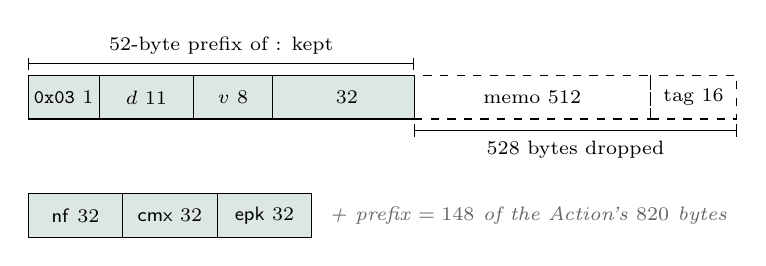
\begin{tikzpicture}[every node/.style={font=\scriptsize},
  b/.style={draw,minimum height=5.5mm,inner sep=2pt,outer sep=0pt,
    anchor=west}]
\node[b,fill=arb!15,minimum width=9mm] (l) at (0,0) {$\mathtt{0x03}$ 1};
\node[b,fill=arb!15,minimum width=12mm] (d) at (l.east) {$d$ 11};
\node[b,fill=arb!15,minimum width=10mm] (v) at (d.east) {$v$ 8};
\node[b,fill=arb!15,minimum width=18mm] (r) at (v.east) {\wbFrseed{} 32};
\node[b,dashed,minimum width=30mm] (m) at (r.east) {memo 512};
\node[b,dashed,minimum width=11mm] (t) at (m.east) {tag 16};
\draw[|-|] ([yshift=1.5mm]l.north west) -- ([yshift=1.5mm]r.north east)
  node[midway,above] {$52$-byte prefix of \wbFenc: kept};
\draw[|-|] ([yshift=-1.5mm]m.south west) -- ([yshift=-1.5mm]t.south east)
  node[midway,below] {$528$ bytes dropped};
\node[b,fill=arb!15,minimum width=12mm] (nf) at (0,-1.5) {\nfsym{} 32};
\node[b,fill=arb!15,minimum width=12mm] (cm) at (nf.east) {\cmx{} 32};
\node[b,fill=arb!15,minimum width=12mm] (ep) at (cm.east) {\epk{} 32};
\node[anchor=west,font=\scriptsize\itshape,text=arbdim] at (ep.east)
  {\ + prefix $= 148$ of the Action's $820$ bytes};
\end{tikzpicture}}
\end{center}
\Write
\begin{enumerate}
  \item compact Action $= \nfsym \,\|\, \cmx \,\|\, \epk \,\|\,
    \wbFenc[0..52)$
  \item $3 \cdot 32 + 52 = 148$ of $820$ bytes
  \item dropped: memo, tag, \wbFout, \cvsym, \rksym, anchor, proof,
    signatures
  \item per block, per pool: end-of-block tree size
\end{enumerate}
\Say
\textbf{What does a light client need from each block?} A compact block
keeps only what three tasks need: detect a payment, detect a spend of
one's own notes, update witnesses.

\textbf{Per Action: \nfsym, \cmx, \epk, and the 52-byte prefix.} Dropped:
memo, tag, \wbFout, \cvsym, \rksym, anchor, proof, signatures ---
528 bytes of \wbFenc{} alone. The compact Action is 148 of the Action's
820 bytes. Each block also states its end-of-block tree size per pool.

\textbf{Bitcoin contrast.} An SPV client downloads headers and asks for
what matches; this client downloads every compact block in range and
asks for no particular output.
\Avoid
\begin{itemize}
  \item ``A few hundred bytes'' for the Action. The Action is 820 bytes;
    its compact form is 148.
\end{itemize}
\src{\emph{Wallet Guide}, ``Compact blocks (ZIP-307)''; ``The deployed
  messages''; ``Omissions and fetch-on-detect''; \emph{Ironwood Guide},
  ``Synchronisation, including from cold storage''}
\end{board}

\begin{board}{Accepting a note without its tag}{exists}
\Write
\begin{enumerate}
  \item $\wbFnp := \mathsf{ciphertext}[0..52) \;\oplus\;
    \mathsf{ChaCha20}_{\wbFkenc}(\mathrm{nonce} = 0)[64..116)$
  \item bare keystream, past block $0$ (the tag key's block)
  \item accept iff: 1. the 52 bytes parse as a compact note plaintext;
    2. recomputed commitment $=$ served \cmx; 3. \esk{} from \wbFrseed{}
    reproduces \epk
  \item commitment binding stands in for the tag
\end{enumerate}
\Say
\textbf{Truncation at 52 bytes discards the Poly1305 tag.} A compact
decryption cannot be authenticated the AEAD way, so the wallet applies
the bare keystream, past block $0$, which the full AEAD reserves for the
tag key.

\textbf{The commitment stands in for the tag.} The wallet accepts iff
the 52 bytes parse as a compact note plaintext, the recomputed
commitment equals the served \cmx, and the \esk{} re-derived from
\wbFrseed{} reproduces \epk. Bob holds neither \cvsym{} nor the binding
signature, so commitment binding is what he relies on: under binding,
no sender can make Bob accept a note the chain did not commit to.

\textbf{Bitcoin contrast.} BIP-37 hands each peer a Bloom filter of the
wallet's scripts; BIP-157 matches a per-block filter locally, then
fetches the matching blocks. Here the ``filter'' is \ivk, applied to
every block, and no match is ever requested.
\src{\emph{Wallet Guide}, ``Compact trial decryption'';\\
  \emph{Ironwood Guide}, ``Recipient: trial decryption and re-derivation''}
\end{board}

\begin{board}{Leaks, in both directions}{none --- privacy of the scan}
\Write
\begin{enumerate}
  \item scan stage: \textbf{less} --- every compact block in range
    fetched; server sees range bounds $+$ timing, never a per-block
    match
  \item after detection: \textbf{more} --- full-transaction fetch names
    an exact txid (BIP-157: a whole block)
  \item ZIP-307 on that fetch: decoys (SHOULD); every transaction of
    any block touched (SHOULD); tell the user (MUST)
  \item deployed libraries: no decoy policy
\end{enumerate}
\Say
\textbf{At the scan stage, less.} Every compact block in a range is
fetched whether or not anything inside opens; the server sees range
bounds and timing, never a per-block match. A BIP-157 client reveals
each block it fetches after a filter hit.

\textbf{After detection, more.} The memo and \wbFout{} live in the full
transaction, which compact blocks omit; fetching it names an exact txid,
where a BIP-157 client names a whole block.

\textbf{ZIP-307 attaches three requirements to that fetch.} Obscure
interest with uninteresting transactions (SHOULD), fetch every
transaction of any block touched (SHOULD), tell the user (MUST). The
deployed client and server libraries ship no decoy policy.

\textbf{Structural, not accidental.} A client that asks for ranges
reveals where it stopped; one that fetches what it detected reveals what
it detected.
\src{\emph{Wallet Guide}, ``Omissions and fetch-on-detect''; ``Leaks in the
  deployed pattern''}
\end{board}

\begin{board}{Placing the note: a position from public data}{exists,
  not twice}
\Write
\begin{enumerate}
  \item $\mathrm{pos}(\text{output } i \text{ of } tx) =
    \text{start-of-block size} + \mathrm{offset}(tx) + i$
  \item start size $=$ stated end-of-block size $-$ the block's own
    outputs
  \item $\mathrm{offset}(tx) =$ outputs of the block's earlier
    transactions
  \item append \emph{every} \cmx; mark own
  \item spend: every compact \nfsym{} vs own unspent nullifiers, locally
\end{enumerate}
\Say
\textbf{Trial decryption tells Bob that an output is his; the tree needs
to know where.} The position is arithmetic on public data, never a
replay: the start size is the stated end-of-block size minus the block's
own outputs, and the offset counts the outputs of the block's earlier
transactions.

\textbf{The size is load-bearing, not a convenience.} The wallet appends
every \cmx{} --- Bob's and everyone else's --- and marks its own; a note
without a position has no witness.

\textbf{A spend of Bob's note is detected the same way.} Every compact
nullifier is compared against the wallet's own unspent nullifiers,
locally.

\textbf{Bitcoin contrast.} An SPV client's branch arrives because its
filter (BIP-37), its block fetch (BIP-157), or --- on Electrum --- the
txid itself named its interest. Bob names nothing; his position is his
own arithmetic.
\Avoid
\begin{itemize}
  \item Calling $\rho$ a tree position. The position is this arithmetic
    on public sizes; $\rho$ never enters it, and the leaf index never
    enters the nullifier.
\end{itemize}
\src{\emph{Wallet Guide}, ``Scanning: spends, positions, and tree sizes'';
  \emph{Ironwood Guide}, ``Synchronisation, including from cold storage''}
\end{board}

\begin{board}{Shards and the cap: a witness without the whole tree}{exists}
\Draw
\begin{enumerate}
  \item Bottom row, five boxes left to right: ``shard 0'', ``shard 1'',
    ``shard 2'', ``shard 3 (Bob's)'' (thick, red, two lines), ``empty
    $\cdots$'' (dashed).
  \item Above each box a small circle, its root; Bob's red, the empty
    one dashed; one stroke from each box up to its circle.
  \item Pair the roots: one circle above shards 0--1, one above 2--3, a
    dashed one above the empty root; join each pair.
  \item One circle above the two pairs; join; a rounded box ``anchor''
    at the top, joined to that circle and dashed to the empty branch.
  \item Right margin, level with the rows: ``$2^{16}$ leaves each'',
    ``one 32-byte root each'', ``the 16-level cap''.
\end{enumerate}
\begin{center}
\resizebox{0.6\textwidth}{!}{%
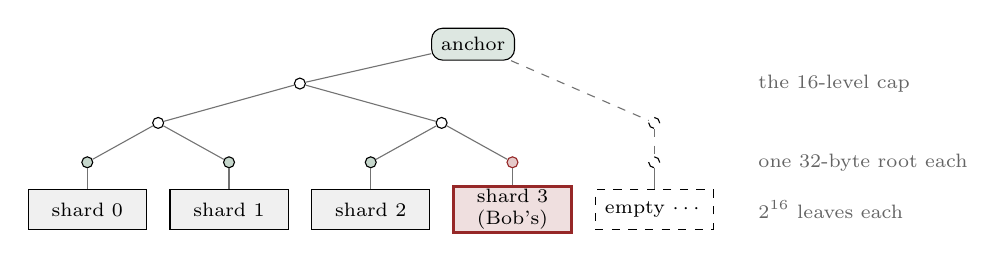
\begin{tikzpicture}[x=1mm,y=1mm,every node/.style={font=\scriptsize},
  sh/.style={draw,minimum width=15mm,minimum height=5mm,inner sep=1pt,
    align=center},
  rt/.style={draw,circle,inner sep=1.4pt},
  ed/.style={black!55}]
\node[sh,fill=black!6] (s0) at (0,0) {shard $0$};
\node[sh,fill=black!6] (s1) at (18,0) {shard $1$};
\node[sh,fill=black!6] (s2) at (36,0) {shard $2$};
\node[sh,fill=arbred!15,draw=arbred,very thick] (s3) at (54,0)
  {shard $3$\\ (Bob's)};
\node[sh,dashed] (s4) at (72,0) {empty $\cdots$};
\node[rt,fill=arb!25] (r0) at (0,6) {};
\node[rt,fill=arb!25] (r1) at (18,6) {};
\node[rt,fill=arb!25] (r2) at (36,6) {};
\node[rt,fill=arbred!25,draw=arbred] (r3) at (54,6) {};
\node[rt,dashed] (r4) at (72,6) {};
\node[rt] (a) at (9,11) {}; \node[rt] (b) at (45,11) {};
\node[rt,dashed] (c) at (72,11) {};
\node[rt] (e) at (27,16) {};
\node[draw,rounded corners,fill=arb!15] (R) at (49,21) {anchor};
\foreach \i in {0,...,4} {\draw[ed] (s\i) -- (r\i);}
\draw[ed] (a)--(r0); \draw[ed] (a)--(r1); \draw[ed] (b)--(r2);
\draw[ed] (b)--(r3); \draw[ed,dashed] (c)--(r4);
\draw[ed] (e)--(a); \draw[ed] (e)--(b); \draw[ed] (R)--(e);
\draw[ed,dashed] (R)--(c);
\node[anchor=west,text=arbdim] at (84,0) {$2^{16}$ leaves each};
\node[anchor=west,text=arbdim] at (84,6) {one $32$-byte root each};
\node[anchor=west,text=arbdim] at (84,16) {the $16$-level cap};
\end{tikzpicture}}
\end{center}
\Write
\begin{enumerate}
  \item depth 32, cut at 16: shards of $2^{16}$ leaves, at most $2^{16}$
    of them, 16-level cap of shard roots
  \item own shard $+$ unfinished tip shard: hashed from leaves
  \item every completed shard: one root from the server
  \item path: low 16 siblings from leaves, high 16 from roots
  \item unbegun shard $=$ per-level constant
\end{enumerate}
\Say
\textbf{Cut the depth-32 tree at half depth.} Shards of $2^{16}$ leaves,
at most $2^{16}$ of them, under a 16-level cap of shard roots.

\textbf{Bob hashes his own shard and takes the rest as roots.} He
hashes his own shard from its leaves and takes every completed shard as
one root from the server; the unfinished tip shard, like his own, is
scanned from leaves. Low 16 siblings come from leaves, high 16 from
roots; an unbegun shard is a per-level constant.

\textbf{Bitcoin contrast.} An SPV client is handed one branch by its
peer. Bob folds his own from public roots and asks for nothing ---
asking for one note's path would say which note is his. Only the anchor
is ever public.
\src{\emph{Ironwood Guide}, ``The wallet's witness: shardtree, shards,
  and the cap''; \emph{Wallet Guide}, ``Client state: shards, cap, and
  retention''}
\end{board}

\begin{board}{Checkpoints: the tree as of a block}{exists}
\Write
\begin{enumerate}
  \item checkpoint at height $h$ $=$ last-leaf position as of block $h$
    $+$ marks dropped since the previous one
  \item uses: fold a path against block $h$'s root; truncate to it on a
    reorganisation
  \item \emph{shared} $=$ present in every pool's tree at that height
  \item bounded recent set $+$ durable ones exempt from pruning
  \item a block appending nothing need not create one
\end{enumerate}
\Say
\textbf{A checkpoint is the wallet's record of its tree at a block
boundary.} It holds the position of the last leaf as of that block, plus
the marks dropped since the previous one, and is identified by the
block's height.

\textbf{Two uses.} Fold a path against that block's root, so a witness
can target any checkpointed block; and truncate the tree back to it
when a reorganisation strikes.

\textbf{Shared means present in every pool's tree.} When one tree gains
a checkpoint at a height, the others gain one too, so a single height
names a state of every tree. A bounded recent set is kept, plus durable
ones exempt from pruning; a block that appends nothing need not create
one.

\textbf{Bitcoin contrast.} Bitcoin Core's checkpoints are hard-coded
block hashes inside the node; these are wallet-local tree snapshots that
consensus never sees.
\src{\emph{Ironwood Guide}, ``The wallet's witness: shardtree, shards,
  and the cap''; \emph{Wallet Guide}, ``Client state: shards, cap, and
  retention''; ``Reorganisation detection and recovery''}
\end{board}

\begin{board}{The frontier as the scan seed}{exists}
\Write
\begin{enumerate}
  \item frontier of a tree of size $n$ $=$ rightmost path: last leaf $+$
    one sibling hash per filled subtree up to the root
  \item wallet birth: frontier of the block \emph{before} the birthday
  \item batch seed: chain state of the block before it, checked against
    the first block's own end-of-block size
  \item contradiction $\to$ batch mis-sequenced; size contradicted by
    the block's contents $=$ continuity error $\to$ reorganisation path
  \item note tree-ready: own shard's block extent $+$ tip range scanned
\end{enumerate}
\Say
\textbf{A frontier is the rightmost path of a tree.} The last leaf plus
one sibling hash per filled subtree on its way to the root: enough to
keep appending, and enough to seed a shard tree.

\textbf{A wallet is born from the frontier of the block before its
birthday.} That frontier summarises every earlier commitment, so no
block below the birthday is ever replayed.

\textbf{Every scanned batch is seeded and checked before any tree is
touched.} The seed is the chain state of the block before the batch,
checked against the first block's own end-of-block size; a contradiction
rejects the batch as mis-sequenced. A size the block's own contents
contradict is the continuity error --- the reorganisation path.

\textbf{A found note is tree-ready before the whole history is.} Once
its own shard's block extent and the tip range are scanned, it is ready.

\textbf{Bitcoin contrast.} A restored Bitcoin wallet also rescans from
its birthday, but needs no tree state: the UTXO set is public, and a
peer answers a filter, or an Electrum server answers by address.
\src{\emph{Wallet Guide}, ``Frontiers as scan seeds''; ``The account
  birthday''; ``Shard completion and spendability''}
\end{board}

\begin{board}{What the server learns: the schedule}{none --- privacy of
  the scan}
\Draw
Three columns: observable, reveals, mitigation status. Rows in order:
\begin{enumerate}
  \item peer IP, connection timing --- endpoint, activity windows --- Tor
    capability; deployment unknown
  \item lowest range start --- approximate account birthday --- none
  \item range boundaries --- scan state and progress --- bucketing
    proposed, unimplemented
\end{enumerate}
\Write
\begin{enumerate}
  \item keys never travel; requests do
  \item ZIP-307's goal: payment-detection privacy against an
    honest-but-curious proxy; spending out of scope
\end{enumerate}
\Say
\textbf{Keys never travel; requests do.} ZIP-307's stated goal is
payment-detection privacy against an honest-but-curious proxy; spending
is outside its scope.

\textbf{The schedule is what leaks.} The peer address and connection
timing give the endpoint and its activity windows; the lowest range
start gives an approximate account birthday; the range boundaries give
scan state and progress. A Tor capability exists, with deployment
unknown; bucketing is proposed and unimplemented; for the birthday
there is nothing.

\textbf{Bitcoin contrast.} A BIP-157 client shows a peer the same kind
of schedule --- which filter ranges it pulls, and when --- and then
every block it fetches on top. Here the content holds and the schedule
leaks.
\src{\emph{Wallet Guide}, ``The stated security model''; ``What never leaves
  the device''; ``Leaks in the deployed pattern''; ``Deployed
  mitigations''}
\end{board}

\begin{board}{What the server learns: the content channels}{none ---
  privacy of the scan}
\Draw
Same three columns. Rows in order:
\begin{enumerate}
  \item fetch after detection --- \textbf{transactions of interest} ---
    decoys a SHOULD; no library policy
  \item submission via the server --- the whole transaction, linked to
    origin --- circuit isolation; deployment unknown
  \item transparent-address calls --- addresses outright --- jitter
    (one-use addresses only)
\end{enumerate}
\Write
\begin{enumerate}
  \item detection stays on the device
  \item three requests carry content, each sent only after the wallet
    decided to
\end{enumerate}
\Say
\textbf{Detection stays on the device; three kinds of request carry
content anyway.} Each is sent only after the wallet itself decided to.

\textbf{The rows.} A fetch after detection names the transactions of
interest, and decoys are a SHOULD with no library policy. A submission
through the server hands it the whole transaction, linked to origin;
circuit isolation exists, deployment unknown. Transparent-address calls
give addresses outright; jitter covers one-use addresses only.

\textbf{Bitcoin contrast.} A BIP-37 client leaks its addresses up to the
false-positive rate, a BIP-157 client its matched blocks; here content
leaks only through what the wallet sends after detecting.
\src{\emph{Wallet Guide}, ``What never leaves the device''; ``Leaks in the
  deployed pattern''; ``The submission channel''; ``Deployed
  mitigations''}
\end{board}

\begin{board}{Mitigations that ship, and the structural reading}{none ---
  privacy of the scan}
\Write
\begin{enumerate}
  \item no request carries key material: heights, hashes, txids,
    transparent addresses, raw transactions only
  \item Tor client with circuit isolation: in the wallet library;
    default routing not determinable
  \item jitter: exponential intervals, shuffled order --- ephemeral
    (ZIP-320) address checks only; none for fetch-on-detect
  \item bucketing: range start rounded down to a multiple of $N$ ---
    ZIP-307's proposal, unimplemented
\end{enumerate}
\Say
\textbf{The baseline holds.} Across the whole service surface no request
carries key material --- only heights, hashes, txids, transparent
addresses, and raw transactions. Trial decryption and nullifier matching
run on the device.

\textbf{Transport.} A Tor client with circuit isolation exists in the
wallet library, so submission need not share a circuit with scanning;
whether any deployed wallet routes through it by default is not
determinable from the sources.

\textbf{Timing.} Exponentially distributed intervals in a shuffled order
--- only for the checks on ephemeral addresses, the one-use transparent
addresses of ZIP-320 payments (Part H). No jitter exists for the
shielded fetch-on-detect.

\textbf{Bucketing} --- rounding a range start down to a multiple of $N$
--- is ZIP-307's own proposal, unimplemented.

\textbf{The reading.} None of this is a property of compact-block
contents, and none of it is inevitable; Tor, bucketing, jitter, and
cover traffic can each change it.
\src{\emph{Wallet Guide}, ``What never leaves the device''; ``Deployed
  mitigations''; ``Summary, and the structural reading''}
\end{board}

\begin{board}{Spending from a light client: the witness and the
  anchor}{exists}
\Write
\begin{enumerate}
  \item witness: 32 siblings, folded on the device from own shard's
    leaves $+$ other shards' roots, against a checkpointed block
  \item the path $=$ private input of the membership clause
  \item anchor: any main-chain root since the pool's activation, no
    window
  \item proving decoupled from broadcasting; appending alters no old
    root
  \item older anchor: no soundness hole; a second spend is the
    nullifier's problem
\end{enumerate}
\Say
\textbf{The witness is folded on the device.} Bob's 32 siblings come
from his shard's leaves and the other shards' roots, against a
checkpointed block; the path is the private input of the membership
clause.

\textbf{The anchor, recalled from Part C.} Any main-chain block's root
since the pool's activation is admissible, no window, so proving is
decoupled from broadcasting; appending alters no old root; an older
anchor is no soundness hole, and a second spend is the nullifier's
problem.

\textbf{Bitcoin contrast.} A Bitcoin input names one txid and index,
and the validator looks it up. The anchor names a tree; the path into
it never leaves the device.
\src{\emph{Ironwood Guide}, ``Anchor choice, reorgs, and the anonymity
  set''; ``The wallet's witness: shardtree, shards, and the cap''}
\end{board}

\begin{board}{Which anchor: the wallet's policy, and whose reasons}{exists}
\Write
\begin{enumerate}
  \item $H$ $=$ target height $=$ tip $+ 1$
  \item anchor $=$ newest shared checkpoint at or below $H - 3$
    (wallet policy, not consensus)
  \item spendable: 3 confirmations trusted, 10 untrusted, from the
    mined block; shard fully scanned; note's block at or below the
    anchor
\end{enumerate}
\Say
\textbf{The anchor is the newest shared checkpoint at or below $H - 3$.}
Here $H$ is the target height, one above the tip. This is wallet
policy, not consensus; ZIP-315's stated reasons and the Guide's
anonymity-set argument are Part C's.

\textbf{Spendable under the same policy.} Three confirmations for
trusted notes, ten for untrusted, counted from the mined block; the
note's shard fully scanned; and its block at or below the anchor.

\textbf{Bitcoin contrast.} A Bitcoin wallet also waits for
confirmations, but which block it ``anchors'' to is nobody's business,
because the input is named either way.
\Avoid
\begin{itemize}
  \item Presenting $H - 3$ as a consensus rule. Consensus admits any
    main-chain anchor since the pool's activation; $H - 3$ is ZIP-315
    wallet policy.
  \item The anonymity-set argument as ZIP-315's. It is the Guide's;
    ZIP-315 states its own reasons (Part C).
\end{itemize}
\src{\emph{Ironwood Guide}, ``Anchor choice, reorgs, and the anonymity
  set''; \emph{Wallet Guide}, ``Confirmations, trust, and spendability'';
  ``Executing the proposal''}
\end{board}

\begin{board}{Expiry and broadcast}{not twice}
\Write
\begin{enumerate}
  \item expiry height (ZIP-203): $0$ $=$ none; included above it $\to$
    block invalid
  \item ZIP-218 recommendation: target $+ 120$
  \item store $\to$ lock inputs $\to$ broadcast, one call
  \item expired unmined $\to$ inputs released, notes spendable again
\end{enumerate}
\Say
\textbf{Every transaction carries an expiry height.} Zero means none; a
block that includes it above that height is invalid. ZIP-218 recommends
target $+ 120$; a uniform delta, like a uniform fee, is not a fingerprint.

\textbf{Store, then broadcast.} The wallet persists the transaction and
locks its inputs before the network sees it, then submits it in one
call. Once expired unmined, it releases its inputs: the notes are
spendable again.

\textbf{Bitcoin contrast.} A stuck transaction has no consensus expiry
--- mempools drop it by policy after a timeout, or RBF or CPFP bumps it.
Here it expires by rule, and its inputs come free.
\src{\emph{Wallet Guide}, ``Expiry (ZIP-203)''; ``Store, then
  broadcast''; ``Expiry and fund availability''}
\end{board}

\begin{board}{The reorganisation case}{exists, not twice}
\Write
\begin{enumerate}
  \item reorganisation past the anchoring block $\to$ anchor invalid
  \item $\to$ truncate to a checkpoint, rescan, rebuild
  \item rebuilt transaction re-reveals the \emph{same} nullifiers
    (deterministic derivation)
  \item re-anchoring, txid unchanged: specified (ZIP-374 v2, anchors in
    authorizing data); wallet support pending
\end{enumerate}
\Say
\textbf{A reorganisation past the anchoring block invalidates the
anchor.} The wallet truncates to a checkpoint, rescans, and rebuilds.

\textbf{The rebuilt transaction re-reveals the same nullifiers.} Their
derivation is deterministic: the notes are the same, so the serial
numbers are.

\textbf{Re-anchoring with the txid unchanged is specified}, in ZIP-374
v2 with anchors in authorizing data; wallet support is pending.

\textbf{Bitcoin contrast.} A reorganised Bitcoin transaction is simply
mined again, since it names its inputs and no anchor. Here a struck
anchor means a rebuild.
\src{\emph{Wallet Guide}, ``Reorganisations: truncate and rescan'';
  ``PCZT v2: deferred anchors and the Ironwood bundle''}
\end{board}

\begin{board}{Three openings on Alice's transaction}{exists}
\Draw
Four columns: ciphertext, opened by, with, yields. Rows in order:
\begin{enumerate}
  \item Action 1, \wbFenc{} --- Bob --- \ivk{} --- $(d,\ 1.5\
    \text{ZEC},\ \wbFrseed)$; the memo, once fetched
  \item Action 2, \wbFenc{} --- Alice --- \wbFivkint{} --- change
    $0.4999$ ZEC, at her internal address
  \item Action 1, \wbFout{} --- Alice --- \ovk{} --- $(\pkd, \esk)$,
    hence Bob's note as he reads it
  \item Action 2, \wbFout{} --- nobody --- (no key) --- random: the
    wallet default seals change under no \ovk
\end{enumerate}
\Write
\begin{enumerate}
  \item Bob: \cmx{} and \epk{} check, position recorded; with \nksym{} a
    nullifier absent from the set; from a stranger: untrusted, 10
    confirmations
  \item Alice: change by trial decryption under \wbFivkint, never
    through \ovk; internal notes trusted: 3 confirmations
  \item Alice: \wbFout{} $\to$ what she sent Bob (sent history; an
    auditor's, given \ovk)
\end{enumerate}
\Say
\textbf{Bob's opening.} His \cmx{} and \epk{} checks pass and the
position is recorded; with \nksym{} he derives a nullifier absent from
the set. From a stranger the note is untrusted: ten confirmations.

\textbf{Alice's change.} She finds it by trial decryption under the
internal scope, never through an outgoing key; internal notes are
trusted: three confirmations.

\textbf{Alice's sent history.} She re-reads what she sent Bob through
\wbFout{} --- her sent history, and an auditor's, given \ovk. The
change Action's \wbFout{} opens for nobody: the wallet default seals
change under no \ovk.

\textbf{Bitcoin contrast.} Bob's payment and Alice's change are the two
outputs everyone reads, and a memo would be an OP\_RETURN.
\Ask
Checkpoint: Bob's light client holds \ivk{} and the 52-byte prefixes:
what can the server still infer, and what would a Bitcoin SPV client
have given away instead?
\begin{itemize}
  \item Still inferred: the endpoint and when it is active; the earliest
    range start, about his birthday; the range bounds, his progress; the
    exact txid, if he fetches the full transaction for the memo; the
    whole transaction before broadcast, if he submits through the same
    server.
  \item Never: which outputs opened, their values, or \ivk{} itself.
  \item A BIP-37 client hands each peer a Bloom filter of its scripts:
    addresses, balance, and graph, up to the false-positive rate. A
    BIP-157 client narrows that to the blocks it fetches after a match
    --- still by asking.
\end{itemize}
\Avoid
\begin{itemize}
  \item Change recovered via \ovk. Alice's change is found by trial
    decryption under \wbFivkint; the wallet default seals change under
    no \ovk{} at all.
  \item A minimum-Actions constant as the reason for the dummy. Action 2
    exists because two outputs need two Actions (Part E); the dummy
    pads the spend list.
  \item Deriving \ovk{} from \ivk. Both derive from \fvk{} (Part D),
    neither from the other.
\end{itemize}
\src{\emph{Ironwood Guide}, ``Recipient: trial decryption and
  re-derivation''; ``The outgoing ciphertext''; \emph{Wallet Guide},
  ``Internal keys: change and auto-shielding''; ``Executing the
  proposal''; ``Confirmations, trust, and spendability''. Checkpoint:
  \emph{Wallet Guide}, ``What never leaves the device''; ``Leaks in the deployed
  pattern''; ``The submission channel''}
\end{board}

%% ---- 09-chain.tex
%% Whiteboard companion, Part H --- The transaction and the turnstile.
%% Drafted from the verified deck fragment draft/09-chain.tex; numbers
%% from compute/h_txsize.py, h_sighash.py, h_pools.py, h_fee.py,
%% h_pczt.py, b_seal.py (outputs pasted above each board, as in the deck).
\newcommand{\wbHvb}{\ensuremath{v_{\mathrm{balance}}}}
\newcommand{\wbHvbi}{\ensuremath{v_{\mathrm{balance}}^{\mathsf{Ironwood}}}}
\newcommand{\wbHvbo}{\ensuremath{v_{\mathrm{balance}}^{\mathsf{Orchard}}}}
\newcommand{\wbHd}[1]{\ensuremath{d_{\mathrm{#1}}}}

\section{Part H --- The transaction and the turnstile}

% compute/h_txsize.py:
%   OrchardAction = 820 B; header = 20 B; signature = 64 B
%   P2PKH input = 150 B; P2PKH output = 34 B
%   proof(a) = 2720 + 2272a: a=1 -> 4992 B; a=2 -> 7264 B
%   Alice v6 (2 Ironwood Actions, all else empty) = 9166 B; proof share =
%   79.2%; sizeProofs compactSize = 3 B
\begin{board}{A v6 transaction beside a Bitcoin transaction}{all four}
\Draw
Two columns headed \emph{Bitcoin} and \emph{Zcash v6}; write the rows
top to bottom:
\begin{enumerate}
  \item header --- version, lock time $\mid$ $+$ version group, branch
    id, expiry height: $20$~B in all
  \item inputs --- outpoint, scriptSig, sequence $\mid$ the same bytes;
    ECDSA over secp256k1, no Taproot; the scriptSig outside the txid
  \item outputs --- value, scriptPubKey $\mid$ the same bytes
  \item Sapling bundle --- --- $\mid$ spends, outputs, Groth16 proofs
  \item Orchard bundle --- --- $\mid$ Actions of the sealed pool
  \item Ironwood component --- --- $\mid$ $a$ Actions at $820$~B; flags,
    \wbHvbi, anchor; one proof of $2720 + 2272a$~B; $a + 1$ signatures
    at $64$~B
\end{enumerate}
\Write
\begin{itemize}
  \item Proof: $2720 + 2272a$~B; for $a = 2$: $7264$~B
  \item Alice: $a = 2$ Actions, $7264$ proof bytes, $9166$ bytes in all
  \item ``One ledger, one transaction type, one asset''
\end{itemize}
\Say
\textbf{In Bitcoin the node reads every field of the transaction: the
header, the inputs, the outputs.} A Zcash v6 transaction keeps those three
parts. The header gains a version group, a branch id and an expiry
height, twenty bytes in all; the inputs are the same bytes, still signed
with ECDSA over secp256k1, no Taproot, the scriptSig outside the txid; the
outputs are the same bytes.

\textbf{The shielded parts are components beside the transparent ones.}
The Sapling bundle carries spends, outputs and Groth16 proofs; the
Orchard bundle carries Actions of the sealed pool; the Ironwood component
carries $a$ Actions at $820$ bytes each, the flags, the balancing field
\wbHvbi, the anchor, one proof of $2720 + 2272a$ bytes and $a + 1$
signatures of $64$ bytes.

\textbf{Alice's payment fills the last component alone.} Two Actions,
$7264$ proof bytes, $9166$ bytes in all; the transparent, Sapling and
Orchard parts are empty.

\textbf{Emphasise: one ledger, one transaction type, one asset.} The
shielded parts are components of the one transaction, not a second
ledger.
\Avoid
Never ``a few hundred bytes'': the numbers are $820$~B per Action, one
proof of $7264$~B for Alice's two Actions, $9166$~B in all.
\src{\emph{Ironwood Guide}, ``The v6 transaction and the Ironwood
  component''; \emph{Crypto Guide}, ``The transparent layer's schemes:
  ECDSA and BIP-340 over secp256k1''}
\end{board}

% compute/h_sighash.py:
%   txid children: v5 4 (hdr, trans, Sap, Orch); v6 5 (+ Irw)
%   signature digest = txid tree with d_trans -> d_transSig; no transparent
%   inputs => identical
\begin{board}{Effecting data, authorizing data: the SegWit shape}{authorised}
\Write
\begin{itemize}
  \item Effecting data $=$ everything under the txid: header; transparent
    outpoints, sequences, outputs; every Action's public fields; flags;
    balancing fields
  \item Authorizing data $=$ what attests to it: proofs, signatures; from
    v6 the three anchors; each scriptSig
  \item Bitcoin: txid $=$ SHA-256d(bytes); SegWit moves the witness out,
    re-commits it through the coinbase
  \item v6: txid $=$ BLAKE2b-256 tree over effecting data;
    $\mathsf{hashAuthDataRoot} \to \mathsf{hashBlockCommitments}$
    (ZIP-244)
  \item Re-anchoring, txid unchanged: specified (ZIP-374 v2), wallet
    support pending
  \item NU7 permits v5 and v6, not v4; the Orchard-pool seal applies
\end{itemize}
\Say
\textbf{Bitcoin's txid is SHA-256d of the bytes, and SegWit moved the
witness out of them,} re-committed through the coinbase. Zcash applies
the same move to everything that attests rather than effects.

\textbf{Effecting data is everything under the txid.} The header; the
transparent outpoints, sequences and outputs; every Action's public
fields; the flags; the balancing fields. Each scriptSig is authorizing
data --- SegWit's move, applied to the legacy input. Authorizing data is
what attests to the effecting data: proofs and signatures, and from v6
the three anchors.

\textbf{A v6 txid is a BLAKE2b-256 tree over the effecting data alone.}
ZIP-244 re-commits the authorizing data through
$\mathsf{hashAuthDataRoot}$, folded into the header's
$\mathsf{hashBlockCommitments}$. Recomputing a proof or a signature
changes nothing the identifier names.

\textbf{Because the anchor is authorizing data, a v6 transaction can be
re-anchored with its txid unchanged:} its membership proof rebased onto a
later root. Say both halves: specified (ZIP-374 v2), wallet support
pending.

\textbf{NU7 permits versions v5 and v6, not v4} (draft ZIP-259).
The Orchard-pool seal applies independently of the version.
\Avoid
Do not present same-txid re-anchoring as deployed: it is specified
(ZIP-374 v2), wallet support pending.
\src{\emph{Ironwood Guide}, ``What the signatures sign: ZIP-244 digests
  and their v6 form''; ``The v6 transaction and the Ironwood component'';
  \emph{Crypto Guide}, ``The transparent layer's hashes'';
  \emph{FlyClient Guide}, ``Why an authorising-data root exists'';
  \emph{Wallet Guide}, ``PCZT v2: deferred anchors and the Ironwood
  bundle''}
\end{board}

% compute/h_sighash.py:
%   node = BLAKE2b-256, 32 B; personalisation carries the 4-byte branch id
%   txid children: v5 4 (hdr, trans, Sap, Orch); v6 5 (+ Irw)
%   signature digest = txid tree with d_trans -> d_transSig; no transparent
%   inputs => identical
%   per-Action partition of C_enc: compact [0:52], memo [52:564], tail
%   [564:]
\begin{board}{The sighash (ZIP-244): a tree of digests}{authorised}
\Draw
\begin{enumerate}
  \item Top centre, one box:
    \begin{gather*}
      \mathsf{txidDigest} = \mathrm{BLAKE2b}\text{-}256\bigl(
        \texttt{ZcashTxHash\_}\,\|\,\mathsf{branchid},\\
        \wbHd{hdr}\,\|\,\wbHd{trans}\,\|\,\wbHd{Sap}\,\|\,
        \wbHd{Orch}\,\|\,\wbHd{Irw}\bigr)
    \end{gather*}
  \item Below it, five boxes left to right, a line from the root to each:
    \wbHd{hdr} (version, expiry); \wbHd{trans} (prevouts, sequences,
    outputs); \wbHd{Sap}; \wbHd{Orch}; \wbHd{Irw} (per Action $\nfsym$,
    $\cmx$, $\epk$, $C_{\mathrm{enc}}$, $\cvsym$, $\rksym$,
    $C_{\mathrm{out}}$; then flags, \wbHvbi).
  \item Under \wbHd{trans}, in red, a box \wbHd{transSig}: hash\_type;
    all inputs' prevouts, amounts, scriptPubKeys, sequences; the outputs;
    the one input signed (transparent signatures only). A dashed red
    arrow from \wbHd{trans} down to it, labelled ``signature digest''.
  \item Bottom right, a dashed red box outside the tree: ``authorizing
    data, outside the tree: proofs, signatures, the anchors''.
\end{enumerate}
\begin{center}
\resizebox{0.6\textwidth}{!}{%
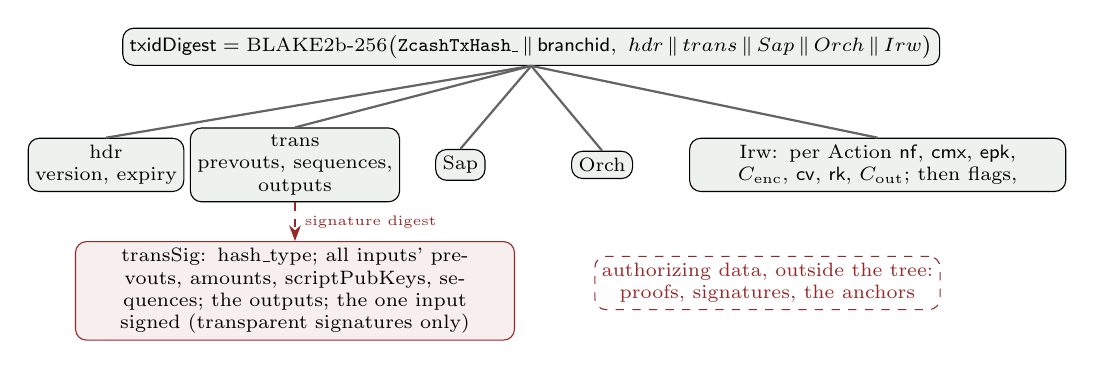
\begin{tikzpicture}[x=1mm,y=1mm,font=\scriptsize,
  nd/.style={draw,rounded corners,inner sep=2.5pt,align=center,fill=arb!8},
  sig/.style={draw,rounded corners,inner sep=2.5pt,align=center,
    fill=arbred!8,draw=arbred},
  auth/.style={draw,dashed,rounded corners,inner sep=2.5pt,align=center,
    draw=arbred,text=arbred},
  e/.style={-,thick,arbdim}]
\node[nd] (root) at (0,0) {$\mathsf{txidDigest} = \mathrm{BLAKE2b}%
  \text{-}256\bigl(\texttt{ZcashTxHash\_}\,\|\,\mathsf{branchid},\
  \wbHd{hdr}\,\|\,\wbHd{trans}\,\|\,\wbHd{Sap}\,\|\,\wbHd{Orch}\,\|\,%
  \wbHd{Irw}\bigr)$};
\node[nd] (hdr) at (-54,-15) {\wbHd{hdr}\\version, expiry};
\node[nd] (tr) at (-30,-15) {\wbHd{trans}\\prevouts, sequences,\\outputs};
\node[nd] (sap) at (-9,-15) {\wbHd{Sap}};
\node[nd] (orch) at (9,-15) {\wbHd{Orch}};
\node[nd,text width=46mm] (irw) at (44,-15) {\wbHd{Irw}: per Action
  $\nfsym$, $\cmx$, $\epk$, $C_{\mathrm{enc}}$, $\cvsym$, $\rksym$,
  $C_{\mathrm{out}}$; then flags, \wbHvbi};
\foreach \c in {hdr,tr,sap,orch,irw} \draw[e] (root.south) -- (\c.north);
\node[sig,text width=54mm] (trs) at (-30,-31) {\wbHd{transSig}:
  hash\_type; all inputs' prevouts, amounts, scriptPubKeys, sequences;
  the outputs; the one input signed (transparent signatures only)};
\draw[-{Stealth[length=2mm]},arbred,dashed] (tr.south) -- (trs.north)
  node[midway,right,font=\tiny,text=arbred]{signature digest};
\node[auth] (au) at (30,-30) {authorizing data, outside the tree:\\
  proofs, signatures, the anchors};
\end{tikzpicture}}
\end{center}
\Write
\begin{itemize}
  \item Every node $=$ one BLAKE2b-256 under its own personalisation; the
    root's carries the branch id
  \item Signature digest $=$ the txid tree with $\wbHd{trans} \to
    \wbHd{transSig}$
  \item No transparent inputs $\Rightarrow$ signature digest $=$ txid
\end{itemize}
\Say
\textbf{Every node of the tree is one BLAKE2b-256 under its own
personalisation.} The root's personalisation carries the branch id, so
the same bytes have a different identity on a parallel chain.

\textbf{The five children are the header digest, the transparent digest,
and one per shielded component.} The Ironwood child commits, per Action,
to $\nfsym$, $\cmx$, $\epk$, $C_{\mathrm{enc}}$, $\cvsym$, $\rksym$ and
$C_{\mathrm{out}}$, then to the flags and \wbHvbi.

\textbf{The signature digest is this tree with \wbHd{trans} swapped for
\wbHd{transSig}.} That child carries the hash\_type, all inputs'
prevouts, amounts, scriptPubKeys and sequences, the outputs, and the one
input being signed --- transparent signatures only. A transaction with
no transparent inputs has nothing to swap: its signature digest \emph{is}
its txid.

\textbf{Emphasise what sits outside the tree:} proofs, signatures, the
anchors --- authorizing data, committed through
$\mathsf{hashAuthDataRoot}$ instead.
\src{\emph{Ironwood Guide}, ``What the signatures sign: ZIP-244 digests
  and their v6 form''; \emph{Wallet Guide}, ``Serialisation and the
  transaction identifier''}
\end{board}

% compute/h_sighash.py:
%   transparent hash_type values: 0x01, 0x02, 0x03, 0x81, 0x82, 0x83 (6;
%   ANYONECANPAY = 0x80 flag); Sapling/Orchard/Ironwood signatures:
%   SIGHASH_ALL = 0x01 always
% compute/h_fee.py: nullifiers = 2; commitments = 2 (one each per Action)
\begin{board}{What the shielded signatures sign}{authorised}
\Write
\begin{itemize}
  \item Per Action: spend-authorisation signature under \rksym; per
    bundle: binding signature under $\mathsf{bvk}$ --- both sign the
    signature digest: every Action's $\nfsym$, $\cmx$, $\cvsym$,
    $\rksym$, ciphertexts; the flags; \wbHvb
  \item Bitcoin hash\_type: ALL, NONE, SINGLE, each with or without
    ANYONECANPAY: six; a transparent Zcash input: exactly those six
  \item Taproot's SIGHASH\_DEFAULT (a seventh spelling of ALL): not in
    ZIP-244
  \item Shielded: SIGHASH\_ALL, always; no shielded ANYONECANPAY
  \item Anchor: not under the signature from v6; the proof carries it as
    a public input (A3)
  \item Alice: no transparent inputs $\Rightarrow$ $2$ spend-auth $+$ $1$
    binding signature all sign her txid
\end{itemize}
\Say
\textbf{In Bitcoin each signer picks a hash\_type.} ALL, NONE, SINGLE,
each with or without ANYONECANPAY: six meaningful values. Taproot adds
SIGHASH\_DEFAULT as a seventh spelling of ALL, which ZIP-244 does not
define. A transparent Zcash input is restricted by consensus to exactly
those six.

\textbf{A shielded signature has one: SIGHASH\_ALL, always.} Each
Action's signature under \rksym{} (spend authorisation) and the bundle's
signature under $\mathsf{bvk}$ (binding) sign the signature digest: every
Action's $\nfsym$, $\cmx$, $\cvsym$, $\rksym$ and ciphertexts, the flags,
\wbHvb. No Action can be transplanted into another transaction, no field
altered. There is no shielded ANYONECANPAY.

\textbf{The anchor is not under the signature from v6, and does not need
to be.} The proof carries it as a public input, clause A3: the signature
attests to the spend, the proof pins the tree.

\textbf{Alice has no transparent inputs.} Her two spend-authorisation
signatures and her binding signature all sign her txid.
\src{\emph{Ironwood Guide}, ``What the signatures sign: ZIP-244 digests
  and their v6 form''; ``What a node verifies, without ever observing the
  note''; \emph{Wallet Guide}, ``Signing''; ``Proving''}
\end{board}

% compute/h_pools.py:
%   fees: shielding 15000, unshielding 15000 zatoshi
%   valueBalanceIronwood: shielding -999985000 = -9.99985 ZEC;
%   unshielding +999985000 = +9.99985 ZEC
\begin{board}{Pools and the doors}{conserved}
\Draw
\begin{enumerate}
  \item Three boxes in a row: \emph{Orchard pool (sealed)} on the left,
    in red; \emph{Ironwood pool} in the centre; \emph{Sapling pool} on
    the right.
  \item Below the Ironwood pool a fourth box, \emph{transparent}.
  \item Above the Ironwood pool the words \emph{coinbase (issuance)},
    with an arrow down into it.
  \item An arrow Orchard $\to$ Ironwood labelled \emph{turnstile}; an
    arrow Sapling $\to$ Ironwood labelled \emph{migration}.
  \item Two vertical arrows between transparent and Ironwood: up,
    labelled \emph{shielding: $\wbHvb < 0$}; down, labelled
    \emph{unshielding: $\wbHvb > 0$}.
  \item Bottom right, a note: ``every arrow: amount public; Sapling's own
    doors omitted: only the Orchard pool is sealed''.
\end{enumerate}
\begin{center}
\resizebox{0.6\textwidth}{!}{%
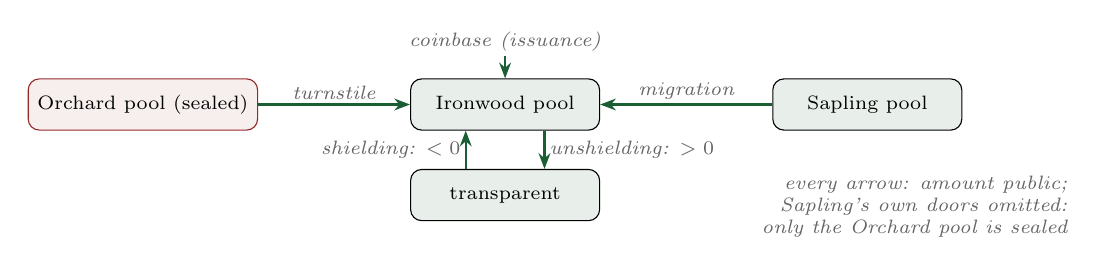
\begin{tikzpicture}[x=1mm,y=1mm,
  pool/.style={draw,rounded corners,minimum width=24mm,minimum height=6.5mm,
    fill=arb!10,font=\scriptsize},
  sealed/.style={pool,fill=arbred!8,draw=arbred},
  flow/.style={-{Stealth[length=2mm]},thick,arb},
  lbl/.style={font=\scriptsize\itshape,text=arbdim,inner sep=1.5pt}]
\node[sealed] (o) at (-46,0) {Orchard pool (sealed)};
\node[pool] (i) at (0,0) {Ironwood pool};
\node[pool] (s) at (46,0) {Sapling pool};
\node[pool] (t) at (0,-11.5) {transparent};
\node[lbl] (cb) at (0,8) {coinbase (issuance)};
\draw[flow] (o) -- (i) node[midway,above,lbl]{turnstile};
\draw[flow] (s) -- (i) node[midway,above,lbl]{migration};
\draw[flow] (cb) -- (i);
\draw[flow] ([xshift=-5mm]t.north) -- ([xshift=-5mm]i.south)
  node[midway,left,lbl]{shielding: $\wbHvb < 0$};
\draw[flow] ([xshift=5mm]i.south) -- ([xshift=5mm]t.north)
  node[midway,right,lbl]{unshielding: $\wbHvb > 0$};
\node[lbl,align=right] at (52,-13) {every arrow: amount public;\\
  Sapling's own doors omitted:\\only the Orchard pool is sealed};
\end{tikzpicture}}
\end{center}
\Write
\begin{itemize}
  \item Shielding: transparent inputs fund $\wbHvbi < 0$; the Actions
    spend dummies, create real notes. Alice shields $10$ ZEC:
    $\wbHvbi = -9.99985$ ZEC printed; her new note not
  \item Coinbase: issuance enters a shielded pool directly; every shielded
    coinbase output decrypts under the all-zero \ovk
  \item Migration: Sapling $\to$ Ironwood; Orchard $\to$ Ironwood through
    the turnstile; both balancing fields cleartext
\end{itemize}
\Say
\textbf{Bitcoin has one pool and needs no doors.} Zcash has several, and
value crosses between them only through doors that print the amount.

\textbf{Shielding.} Transparent inputs fund a negative \wbHvbi; the
Actions spend dummies and create real notes. Alice shields $10$ ZEC:
$\wbHvbi = -9.99985$ ZEC is printed, her new note is not. Wallets shield
automatically, to an internal address.

\textbf{Coinbase.} Issuance enters a shielded pool directly, but every
shielded coinbase output must decrypt under the all-zero \ovk: anyone can
read what issuance entered which pool.

\textbf{Migration.} Sapling or the sealed Orchard pool to Ironwood, the
latter through the turnstile; both balancing fields are cleartext.

\textbf{Emphasise: every arrow on the board prints its amount.} Only the
Orchard pool is sealed; Sapling's own doors are left off the drawing.
\src{\emph{Ironwood Guide}, ``The doors: shielding, coinbase, migration'';
  ``The turnstile and migration''}
\end{board}

% compute/h_pools.py:
%   Alice's deposit = 999985000 = 9.99985 ZEC; Bob's output = 999970000 =
%   9.9997 ZEC = 10 ZEC less two fees
%   pool balance after both, if the pool held only Alice's deposit: 0
%   zatoshi; one zatoshi more out -> -1 -> a block containing Bob's spend
%   would be invalid
\begin{board}{The turnstile (ZIP-209): audited at the boundary}{conserved}
\Write
\begin{itemize}
  \item $\mathsf{balance}_{P} := -\sum_{\mathrm{tx}}
    \wbHvb^{P}(\mathrm{tx}) \ge 0$ in every block, for
    $P \in \{\mathsf{Sap}, \mathsf{Orch}, \mathsf{Irw}\}$
  \item Sprout: $\sum \mathtt{vpub\_old} - \sum \mathtt{vpub\_new}$;
    transparent: the UTXO sum; lockbox: its accrued subsidy
  \item A block driving any balance negative, or the total past
    $\mathsf{MAX\_MONEY}$: invalid
  \item Inside a pool: counterfeit undetectable. At the exit: capped at
    what the pool publicly holds
  \item Example: pool holds only Alice's $9.99985$ ZEC; Bob's $+9.99985$
    ZEC exit empties it exactly; one zatoshi more $\Rightarrow$ block
    invalid
\end{itemize}
\Say
\textbf{Bitcoin audits by summing every coin.} Inside a shielded pool no
check sums the notes, so a counterfeit is undetectable there. Sprout's
original proof system had exactly such a flaw (Part G): a forged proof
mints silently.

\textbf{The mechanism is a public balance per pool, checked at the
door.} The balance of pool $P$ is minus the sum of its balancing fields
over every transaction, and it must stay non-negative in every block, for
the Sapling, Orchard and Ironwood pools. Every pool has a public balance
under this rule: Sprout's is $\sum \mathtt{vpub\_old} - \sum
\mathtt{vpub\_new}$, the transparent pool's the UTXO sum, the lockbox's
its accrued subsidy. A block driving any negative, or the total past
$\mathsf{MAX\_MONEY}$, is invalid.

\textbf{At the exit the damage is capped.} A forger can withdraw at most
what the pool publicly holds. The Sapling pool still rests on its Groth16
ceremony; the turnstile bounds it.

\textbf{On the running example:} had the Ironwood pool held only Alice's
deposit of $9.99985$ ZEC, Bob's $+9.99985$ ZEC exit would empty it
exactly; one zatoshi more and his block is invalid.

\textbf{Emphasise: Zcash audits each pool at its door,} not inside.
\Avoid
Never ``the pool is auditable'': nothing sums the notes inside; only the
balance at the door is public, and a counterfeit inside is undetectable
until it tries to leave. Never ``no ceremony'' without the caveat: the
Sapling pool still rests on its Groth16 ceremony, bounded by the
turnstile.
\src{\emph{Ironwood Guide}, ``Pool balances: ZIP-209 and its Ironwood
  analogue''; ``The turnstile and migration''; ``Prospective breaks: the
  discrete-log integrity stack''; ``Lineage: three generations of
  shielded proof''; ZIP-209; protocol specification, ``Chain Value Pool
  Balances''}
\end{board}

% compute/b_seal.py:
%   flags byte: Orchard 0b011 (bit 2 = 0b100 clear), Ironwood 0b111 (bit 2
%   set)
\begin{board}{Why the Orchard pool is sealed}{conserved}
\Write
\begin{itemize}
  \item Three rules: no issuance; no circulation
    ($\mathsf{enableCrossAddress} = 0$); no entry ($\wbHvbo \ge 0$) ---
    whatever the transaction version
  \item Legacy note, lead byte $\mathtt{0x02}$: not quantum-recoverable.
    Ironwood note, lead byte $\mathtt{0x03}$, hashed \rcm: recoverable
  \item Orchard pool balance can only fall; every exit metered in
    cleartext by \wbHvbo
  \item Bitcoin never retires an output type; a P2PK coin spends forever
\end{itemize}
\Say
\textbf{Bitcoin never retires an output type; a P2PK coin spends
forever.} Here a pool can be sealed by three rules and drained through a
metered gate.

\textbf{The seal is the three rules of Parts C and E.} They bind
whatever the transaction version: no issuance; no circulation,
$\mathsf{enableCrossAddress} = 0$; no entry, $\wbHvbo \ge 0$.

\textbf{The reason is Part F's one note-level difference.} A legacy note,
lead byte $\mathtt{0x02}$, is not quantum-recoverable; an Ironwood note,
lead byte $\mathtt{0x03}$ with the hashed \rcm, is. So consensus stops
the old notes circulating and funnels their value out through the
turnstile, while owners can still spend what they hold.

\textbf{The turnstile is the seal's accounting shape.} The Orchard pool's
balance can only fall, every exit metered in cleartext by \wbHvbo, so the
legacy pool drains through a public gate.
\src{\emph{Ironwood Guide}, ``The seal: three rules''; ``One circuit,
  one verifying key''; ``ZIP-2005: quantum recoverability''; ``Pool
  balances: ZIP-209 and its Ironwood analogue''}
\end{board}

% compute/h_fee.py:
%   Actions = 2; logical_actions = 2; fee = 5000 * max(2, 2) = 10000 zatoshi
%   one-Action shape padded to two: fee unchanged = 10000
%   shielding, 1 P2PKH input + 2 Actions: logical = 3 -> fee 15000
\begin{board}{Fees (ZIP-317): a function of the public shape}{conserved}
\Write
\begin{align*}
  \mathit{fee} &= 5000 \cdot \max(2,\ \mathit{logical\_actions})
  \quad\text{zatoshi} \\[2pt]
  \mathit{logical\_actions} &=
  \max\Bigl(\Bigl\lceil \tfrac{\text{in bytes}}{150} \Bigr\rceil,
            \Bigl\lceil \tfrac{\text{out bytes}}{34} \Bigr\rceil\Bigr)
  + 2\,\mathit{nJoinSplit}_{\mathrm{Sprout}} \\
  &\quad + \max(\mathit{spends}, \mathit{outputs})_{\mathrm{Sap}}
  + \mathit{nActions}_{\mathrm{Orch}}
  + \mathit{nActions}_{\mathrm{Irw}}
\end{align*}
\begin{itemize}
  \item Divisors: standard P2PKH input $150$~B, output $34$~B
  \item Alice: two Actions, $5000 \cdot \max(2, 2) = 10\,000$ zatoshi
  \item One Action padded to two: $10\,000$, the same
  \item Shielding with one P2PKH input: $1 + 2 = 3$ actions, $15\,000$
\end{itemize}
\Say
\textbf{In Bitcoin the node reads the fee by subtraction, inputs minus
outputs, both in plaintext.} Here the amounts are hidden, so the fee must
be a function of what is public: the shape of the transaction.

\textbf{The fee is $5000$ zatoshi per logical action, with a floor of
two.} Logical actions count, per pool: transparent, the larger of input
bytes over $150$ and output bytes over $34$, each rounded up; two per
Sprout JoinSplit; Sapling, the larger of spends and outputs; Orchard and
Ironwood, the number of Actions. Sum them.

\textbf{The divisors are the standard P2PKH input and output.} One
typical transparent input or output weighs one action, and a fatter
script pays in proportion. An Action spends one note \emph{and} creates
one, so it is counted once --- charging inputs and outputs separately
would tax the padding.

\textbf{Alice pays $10\,000$ zatoshi:} two Actions, $5000 \cdot \max(2,
2)$. A one-Action payment padded to two pays the same. A shielding
transaction with one P2PKH input counts $1 + 2 = 3$ actions and pays
$15\,000$.
\Avoid
Do not give the fee's floor of two as the reason for Alice's dummy: she
has two Actions because she has two outputs (Bob and her change); the
dummy pads her single spend to match. The floor is the fee's grace
window, not the padding rule.
\src{\emph{Wallet Guide}, ``The conventional fee''; ``The fee is computed
  on padded counts''}
\end{board}

% compute/h_fee.py:
%   ZIP-317 template: block_unpaid_action_limit = 50; weight_ratio_cap = 4
\begin{board}{Fees (ZIP-317): why a convention, and who enforces
  it}{conserved}
\Write
\begin{itemize}
  \item Computable from public fields alone
  \item Uniform across wallets: not a fingerprint; padding to two is free
    (grace window $= 2$)
  \item A convention, not consensus: relay at least the fee; template by
    fee ratio, capped at $4\times$; at most $50$ unpaid actions per block
  \item Bitcoin: a market --- bid per virtual byte and coin selection
    vary; both fingerprints
\end{itemize}
\Say
\textbf{Bitcoin runs a fee market.} The bid per virtual byte, and the
coin selection behind it, vary by wallet and moment --- and both are read
as fingerprints. Zcash flattens the market on purpose.

\textbf{Computable from public fields alone.} A fee that depended on
which notes were spent or what change came back would print that data in
the amount paid.

\textbf{Uniform across wallets.} Every wallet is expected to pay exactly
this fee, so the fee is not a fingerprint. Padding to two Actions is free
by design: the grace window is two.

\textbf{A convention, not consensus.} Nodes relay transactions paying at
least it; the recommended block template picks among those by fee ratio,
capped at $4\times$, and admits at most $50$ unpaid actions per block.
Overpaying beyond $4\times$ buys no further priority.
\src{\emph{Wallet Guide}, ``The conventional fee''; ``Relay, mempool,
  and block template''}
\end{board}

% compute/h_fee.py:
%   Actions = 2; logical_actions = 2; fee = 5000 * max(2, 2) = 10000 zatoshi
%   change = 49990000 zatoshi = 0.4999 ZEC; valueBalanceIronwood = +10000
%   zatoshi = fee
%   nullifiers = 2; commitments = 2 (one each per Action)
% compute/h_txsize.py: Alice v6 = 9166 B, proof 7264 B (79.2%)
\begin{board}{The public face of Alice's transaction}{all four}
\Draw
Two columns, \emph{public field} and \emph{Alice pays Bob $1.5$ ZEC from
a $2$ ZEC note}; write the rows top to bottom:
\begin{enumerate}
  \item version --- v6; transparent, Sapling and Orchard parts empty
  \item Ironwood Actions --- $2$ (one real spend, one dummy; shuffled)
  \item nullifiers, commitments --- $2$ and $2$
  \item \wbHvbi{} --- $+10\,000$ zatoshi $=$ the fee
  \item anchor --- the Ironwood root at the newest shared checkpoint at or
    below $H - 3$
  \item expiry --- target height $+\,120$ blocks, about $50$ minutes
  \item signatures --- $2$ spend-authorisation $+$ $1$ binding
  \item size --- $9166$ bytes, $7264$ of them proof
\end{enumerate}
\Write
\begin{itemize}
  \item Bitcoin prints: input coin, both amounts, both scripts, fee by
    subtraction
  \item Here printed: the fee alone, as \wbHvbi
  \item Inside the commitments: $2$ ZEC, $1.5$ ZEC, $0.4999$ ZEC change,
    both addresses
\end{itemize}
\Say
\textbf{Bitcoin prints the same payment as the input coin, both amounts,
both scripts and, by subtraction, the fee.} Here the fee alone is
printed, as \wbHvbi.

\textbf{Walk the table.} Version v6, with the transparent, Sapling and
Orchard parts empty. Two Ironwood Actions, one real spend and one dummy,
shuffled. Two nullifiers and two commitments. The balancing field
$+10\,000$ zatoshi, which is the fee. The anchor is the Ironwood root at
the newest shared checkpoint at or below $H - 3$. ZIP-218 recommends expiry
at target height $+\,120$ blocks, about $50$ minutes. Two spend-authorisation signatures
and one binding signature. Then $9166$ bytes, $7264$ of them proof.

\textbf{Emphasise what stays inside the commitments:} the $2$ ZEC, the
$1.5$ ZEC, the $0.4999$ ZEC change and both addresses.
\Avoid
Never ``the proof hides sender and receiver'': the amounts and addresses
stay inside the commitments; the proof only attests to the statement.
Never ``a few hundred bytes'': $9166$ bytes, $7264$ of them proof. Do not
give a two-Action minimum as the reason for the dummy: two outputs need
two Actions, and the dummy pads the single spend.
\src{\emph{Ironwood Guide}, ``The v6 transaction and the Ironwood
  component''; ``Anchor choice, reorgs, and the anonymity set'';
  ``Conservation without disclosure: value commitments and the binding
  signature''; \emph{Wallet Guide}, ``Padding, dummies, and shuffling'';
  ``Expiry (ZIP-203)''}
\end{board}

\begin{board}{The privacy sliders: pool, address type, timing}{all four}
\Write
\begin{itemize}
  \item Pool: transparent leg prints its amount as \wbHvb; fully shielded
    prints the fee and nothing else
  \item Address type: unified address $=$ bundle of receivers; wallet
    MUST use the most preferred it supports: Orchard-protocol (Ironwood
    pool) $>$ Sapling $>$ transparent. TEX address $\Rightarrow$ two
    transactions via an ephemeral transparent output, both public
  \item Timing: ZIP-218 recommends expiry $=$ target $+\,120$ blocks.
    Migration: denominations $m \cdot 10^{k}$ ZEC, $m \in \{1, 2, 5\}$;
    anchors and expiries from shared grids
  \item ``Uniformity is the strategy''
\end{itemize}
\Say
\textbf{Bitcoin has the address-type slider and the timing slider; it has
no pool slider, because it has one plaintext ledger.}

\textbf{Pool.} A transparent leg prints its amount as \wbHvb; fully
shielded prints the fee and nothing else. The slider is the sender's, set
by which funds and which receiver she uses.

\textbf{Address type.} A unified address bundles receivers; the sender's
wallet MUST use the most preferred one it supports: Orchard-protocol,
into the Ironwood pool, over Sapling over transparent. A TEX address
demands transparent funds, so the wallet builds two transactions through
an ephemeral transparent output --- both public.

\textbf{Timing.} ZIP-218 recommends expiry at target $+\,120$ blocks:
an idiosyncratic delta fingerprints a transaction as an
idiosyncratic fee would. Migration wallets split value into canonical
denominations $m \cdot 10^{k}$ ZEC, $m \in \{1, 2, 5\}$, and draw anchors
and expiries from shared grids for the same reason.

\textbf{Emphasise: uniformity is the strategy.} The defaults protect only
while everyone keeps them.
\src{\emph{Wallet Guide}, ``Unified addresses''; ``Input selection'';
  ``Expiry (ZIP-203)''; \emph{Ironwood Guide}, ``Scheduled
  Orchard-to-Ironwood migration (ZIP-318)''}
\end{board}

% compute/h_pczt.py:
%   ZIP-374 roles: 10 -> Creator, Constructor, IO Finalizer, Updater,
%   Prover, Signer, Combiner, Redactor, Spend Finalizer, Transaction
%   Extractor
%   PSBT roles (BIP 174/370): 7; roles PCZT adds: IO Finalizer, Prover,
%   Redactor
\begin{board}{PSBT $\to$ PCZT (ZIP-374): the unfinished
  transaction}{authorised}
\Write
\begin{itemize}
  \item PSBT (BIP-174 $+$ BIP-370): Creator, Constructor, Updater, Signer,
    Combiner, Input Finalizer, Transaction Extractor
  \item PSBT cannot carry shielded: no shielded spends/outputs; no proof
    distinct from a signature; tolerates unknown fields
  \item PCZT $=$ PSBT roles $+$ IO Finalizer, Redactor, Prover; ten roles
  \item ``Proving is delegated, signing is not''
\end{itemize}
\Say
\textbf{Bitcoin passes an unfinished transaction between roles: PSBT.}
BIP-174, plus BIP-370's Constructor: Creator, Constructor, Updater,
Signer, Combiner, Input Finalizer, Transaction Extractor. Hardware
wallets and multisig live on it.

\textbf{A PSBT cannot carry a shielded transaction.} No representation
for shielded spends and outputs; no notion of a proof distinct from a
signature; and it tolerates unknown fields --- unacceptable for a signer
that must understand everything it authorises.

\textbf{A PCZT keeps the PSBT role structure and adds Zcash's own.} Among
them an IO Finalizer, which declares the inputs and outputs complete and
derives the binding-signature key; a Redactor, which strips what later
parties need not see; and a Prover. Ten roles in all.

\textbf{Emphasise: proving is delegated, signing is not.} The Prover has
no PSBT counterpart because a hardware signer cannot compute a Halo 2
proof, and a proof needs no spending key. Signers can be fully offline;
the format carries everything they need.
\Avoid
No timing claims: say that a hardware signer cannot compute a Halo 2
proof, not how long a proof takes anywhere.
\src{\emph{Wallet Guide}, ``Partially created transactions (PCZT)'';
  ``Roles and lifecycle''}
\end{board}

% compute/h_pczt.py:
%   Signer holds/needs (5): ask; alpha; rk (to check ask + alpha); sighash
%   (computed from the effecting data); the spend's public fields and,
%   unless redacted, the note fields to verify nf, cv, cmx
%   Prover needs (6): fvk; recipient, value, rho, rseed; witness; alpha;
%   rcv; anchor; no spending key
\begin{board}{Signer versus Prover}{authorised}
\Draw
Two columns headed \emph{Signer} and \emph{Prover}; write the rows top to
bottom:
\begin{enumerate}
  \item holds --- \asksym{}, spend authority $\mid$ \fvk{}, no spending
    key
  \item reads from the PCZT --- $\alpha$, \rksym; the spend's public
    fields and, unless redacted, its note fields $\mid$ the note ($\gd$,
    $\pkd$, $v$, $\rho$, $\mathsf{rseed}$), the witness, $\alpha$, \rcv,
    the anchor
  \item computes --- the sighash from the effecting data; $\rsk = \asksym
    + \alpha$, checks it matches \rksym, signs $\mid$ one Halo 2 proof
    over all Actions; anchor and flags as public inputs
  \item verifies first --- $\nfsym$, $\cvsym$, $\cmx$ against the note
    fields: exactly what it authorises $\mid$ \fvk{} owns each note;
    $\rho_{\mathrm{new}} = \nfsym_{\mathrm{old}}$
  \item learns --- what it signs $\mid$ the notes' private data, not
    authority
\end{enumerate}
\Write
\begin{itemize}
  \item $\rsk = \asksym + \alpha$; check against \rksym{} before signing
  \item $\rho_{\mathrm{new}} = \nfsym_{\mathrm{old}}$
  \item Either role runs without the other; the Prover never sees
    \asksym; the Signer may see the note data, or have it redacted
\end{itemize}
\Say
\textbf{In Bitcoin there is no proof distinct from the signature, so the
signer is the only role that attests.} Here proof and signature are
separate artefacts with separate secrets, and the table shows how little
the two roles share.

\textbf{The Signer holds \asksym, the spend authority.} It reads $\alpha$
and \rksym{} from the PCZT, plus the spend's public fields and, unless
redacted, its note fields. It computes the sighash from the effecting
data and $\rsk = \asksym + \alpha$, checks that this matches \rksym, and
signs. Before signing it verifies $\nfsym$, $\cvsym$ and $\cmx$ against
the note fields: exactly what it authorises. It learns what it signs.

\textbf{The Prover holds \fvk{} and no spending key.} It reads the note
($\gd$, $\pkd$, $v$, $\rho$, $\mathsf{rseed}$), the witness, $\alpha$,
\rcv{} and the anchor. It computes one Halo 2 proof over all Actions,
with the anchor and flags as public inputs. First it checks that \fvk{}
owns each note and that $\rho_{\mathrm{new}} = \nfsym_{\mathrm{old}}$. It
learns the notes' private data, not authority.

\textbf{Emphasise:} either role can run without the other; the Prover
never sees \asksym; the Signer may see the note data, or have it
redacted.
\Avoid
Re-randomisation is additive: $\rsk = \asksym + \alpha$, never
$[\alpha]\cdot\aksym$. The seed $\rho$ is a per-note uniqueness value,
$\rho_{\mathrm{new}} = \nfsym_{\mathrm{old}}$, not the note's position in
the tree.
\src{\emph{Wallet Guide}, ``Signing''; ``Proving''}
\end{board}

% compute/h_pczt.py: ZIP-374 roles: 10; roles PCZT adds: IO Finalizer,
%   Prover, Redactor
% compute/h_pools.py:
%   fees: shielding 15000, unshielding 15000 zatoshi
%   Alice's deposit = 999985000 = 9.99985 ZEC; Bob's output = 999970000 =
%   9.9997 ZEC = 10 ZEC less two fees
%   valueBalanceIronwood: shielding -999985000 = -9.99985 ZEC;
%   unshielding +999985000 = +9.99985 ZEC
\begin{board}{PCZT: where it stands}{authorised}
\Write
\begin{itemize}
  \item From v6: signatures commit to no anchor $\Rightarrow$ sign today,
    anchor, witness and prove at broadcast
  \item Delegating the Prover reveals note data, never spend authority;
    a Redactor strips what a later party need not see
  \item Bins: ZIP Draft; format released as a library; deployed wallet
    pipeline drives the roles end to end (Ironwood sent-output records
    not yet stored: backend gap)
  \item $+$ FROST (Part I): ``no script, so no multisig and no hardware
    wallets'' --- closed
\end{itemize}
\Say
\textbf{From v6 the Signer and the Prover are independent even of the
anchor.} Signatures commit to no anchor, so a wallet can sign today and
anchor, witness and prove at broadcast.

\textbf{Delegating the Prover reveals the notes' private data to the
delegate, never spend authority.} A Redactor strips what a later party
need not see.

\textbf{Bins.} The ZIP is Draft; the format is released as a library; the
deployed wallet pipeline drives the roles end to end --- it builds the
PCZT, hands it out for proving and signing, and extracts and stores the
result. Ironwood sent-output records are not yet stored: a backend gap,
not a format limit.

\textbf{Emphasise: with FROST threshold signing (Part I) this closes the
objection ``no script, so no multisig and no hardware wallets''.} The
roles carry both.
\Ask
Alice shields $10$ ZEC; the next day Bob unshields $9.9997$ ZEC. What can
a chain analyst conclude, and what can they not?

\emph{Conclude.} Two cleartext balancing fields, exact to the zatoshi:
$-9.99985$ ZEC entered, $+9.99985$ ZEC left --- $10$ ZEC less two
conventional fees of $15\,000$ zatoshi; the heights; the transparent
addresses on each side; that the amounts match exactly and the times are
close.

\emph{Not conclude.} That Bob's coins were Alice's. Her commitment hides
her note; his nullifier is keyed by his \nksym; his candidate set is
every leaf under his anchor. Her note may still be resting.

Bitcoin would have handed over the path; Zcash hands over a correlation.
Canonical denominations and shared timing grids exist because that
correlation is evidence.
\Avoid
Never ``the pool is auditable'': the analyst reads two door amounts and a
correlation, nothing inside the pool.
\src{\emph{Wallet Guide}, ``Partially created transactions (PCZT)'';
  ``Combining, redaction, and privacy''; ``The deployed wallet
  pipeline''; ``PCZT v2: deferred anchors and the Ironwood bundle'';
  \emph{Ironwood Guide}, ``The doors: shielding, coinbase, migration'';
  ``Anchor choice, reorgs, and the anonymity set''; ``The nullifier, and
  the loop back to minting''; ``Scheduled Orchard-to-Ironwood migration
  (ZIP-318)''}
\end{board}

%% ---- 10-consensus.tex
%% Whiteboard companion, Part K --- Consensus: why one fork wins, and what
%% the chain must remember. Drafted from the verified deck fragment
%% draft/10-consensus.tex; numbers from compute/k_catchup.py (outputs
%% pasted above each board, as in the deck).

%% Block tree: two panels, tied branches and their resolution.
\newcommand{\wbKtree}{%
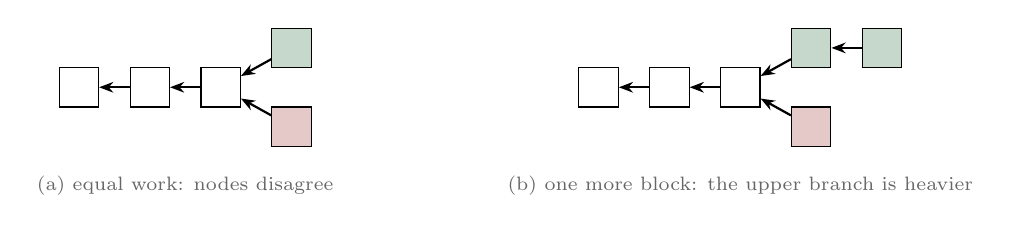
\begin{tikzpicture}[
  blk/.style={draw, rectangle, minimum width=5mm, minimum height=5mm,
    inner sep=0pt, fill=white},
  hon/.style={blk, fill=arb!25},
  att/.style={blk, fill=arbred!25},
  lnk/.style={-{Stealth[length=1.8mm]}, thick},
  lbl/.style={font=\scriptsize, text=black!60},
]
\begin{scope}
\node[blk] (g) at (0,0) {};
\node[blk] (b1) at (0.9,0) {};
\node[blk] (b2) at (1.8,0) {};
\node[hon] (c1) at (2.7,0.5) {};
\node[att] (d1) at (2.7,-0.5) {};
\draw[lnk] (b1) -- (g); \draw[lnk] (b2) -- (b1);
\draw[lnk] (c1) -- (b2); \draw[lnk] (d1) -- (b2);
\node[lbl, anchor=north] at (1.35,-1.0) {(a) equal work: nodes disagree};
\end{scope}
\begin{scope}[xshift=6.6cm]
\node[blk] (g) at (0,0) {};
\node[blk] (b1) at (0.9,0) {};
\node[blk] (b2) at (1.8,0) {};
\node[hon] (c1) at (2.7,0.5) {};
\node[hon] (c2) at (3.6,0.5) {};
\node[att] (d1) at (2.7,-0.5) {};
\draw[lnk] (b1) -- (g); \draw[lnk] (b2) -- (b1);
\draw[lnk] (c1) -- (b2); \draw[lnk] (c2) -- (c1); \draw[lnk] (d1) -- (b2);
\node[lbl, anchor=north] at (1.8,-1.0) {(b) one more block: the upper
  branch is heavier};
\end{scope}
\end{tikzpicture}}

%% The deficit walk: two seeded runs from z = 2 (compute/k_catchup.py).
\newcommand{\wbKwalk}{%
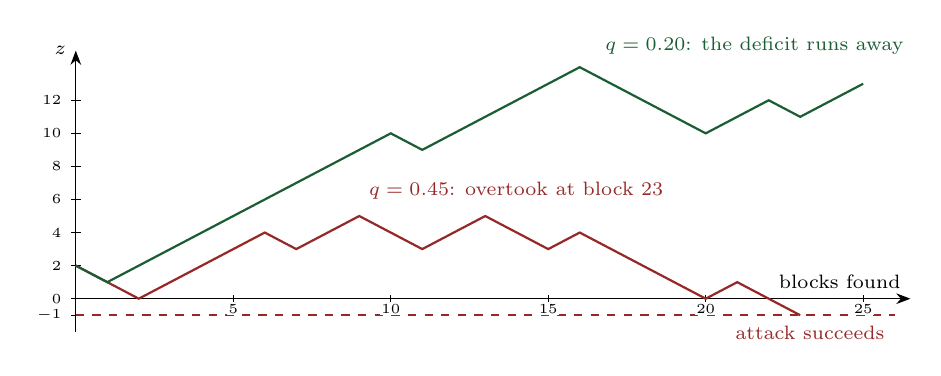
\begin{tikzpicture}[x=0.40cm, y=0.21cm]
\draw[-{Stealth[length=1.8mm]}] (0,-2) -- (0,15)
  node[left, font=\scriptsize] {$z$};
\draw[-{Stealth[length=1.8mm]}] (0,0) -- (26.5,0)
  node[above left, font=\scriptsize] {blocks found};
\foreach \y in {-1, 0, 2, 4, 6, 8, 10, 12}
  \draw (0.15,\y) -- (-0.15,\y) node[left, font=\tiny] {$\y$};
\draw[dashed, thick, arbred] (0,-1) -- (26,-1)
  node[below left, font=\scriptsize, text=arbred] {attack succeeds};
\foreach \x in {5, 10, 15, 20, 25}
  \draw (\x,0.2) -- (\x,-0.2) node[below, font=\tiny, fill=white,
    inner sep=0.6pt] {$\x$};
\draw[thick, arbred] plot coordinates {(0,2) (1,1) (2,0) (3,1) (4,2)
  (5,3) (6,4) (7,3) (8,4) (9,5) (10,4) (11,3) (12,4) (13,5) (14,4)
  (15,3) (16,4) (17,3) (18,2) (19,1) (20,0) (21,1) (22,0) (23,-1)};
\node[font=\scriptsize, text=arbred, anchor=south west] at (9,5.4)
  {$q = 0.45$: overtook at block $23$};
\draw[thick, arb] plot coordinates {(0,2) (1,1) (2,2) (3,3) (4,4) (5,5)
  (6,6) (7,7) (8,8) (9,9) (10,10) (11,9) (12,10) (13,11) (14,12) (15,13)
  (16,14) (17,13) (18,12) (19,11) (20,10) (21,11) (22,12) (23,11)
  (24,12) (25,13)};
\node[font=\scriptsize, text=arb, anchor=south west] at (16.5,14.2)
  {$q = 0.20$: the deficit runs away};
\end{tikzpicture}}

\section{Part K --- Consensus: why one fork wins, and what the chain
  must remember}

\begin{board}{Bitcoin's chain rule, weighed in work}{not twice}
\Draw
\begin{enumerate}
  \item Panel (a): three white boxes in a row; an arrow from the second
    box back to the first and from the third back to the second (a block
    points at its parent).
  \item Right of the third box, two boxes one above the other, the upper
    shaded green, the lower shaded red; an arrow from each back to the
    third box.
  \item Caption under the panel: ``(a) equal work: nodes disagree''.
  \item Panel (b), to the right: the same five boxes, plus a sixth green
    box right of the upper green one, with an arrow back to it.
  \item Caption: ``(b) one more block: the upper branch is heavier''.
\end{enumerate}
\begin{center}
\resizebox{0.6\textwidth}{!}{\wbKtree}
\end{center}
\Write
\begin{itemize}
  \item work of a block $= \lfloor 2^{256} /
    (\mathsf{ToTarget}(\mathtt{nBits}) + 1) \rfloor$
  \item best valid chain $=$ greatest total work; ties $\to$ the block
    received first
  \item ``longest'' $=$ ``most work'' only at constant difficulty
  \item nothing marks a chain as final
\end{itemize}
\Say
\textbf{In Bitcoin every block names its parent, so the node holds a
tree of blocks,} and Zcash keeps the same rule. Each branch is one
consistent history, and sibling branches may conflict.

\textbf{A branch is weighed in work, not counted in blocks.} The work
of a block is the first line on the board; the best valid chain has the
greatest total work; ties go to the block received first.

\textbf{Bitcoin: the same rule.} ``Longest'' equals ``most work'' only
at constant difficulty.

\textbf{Emphasise: nothing marks a chain as final.} A heavier branch
wins however deep the fork; the rest of this part measures how likely
that is.
\Avoid
``Ties go to the block received first'' as deployed behaviour: that is
the specification's rule and Rosenfeld's; the deployed node departs
from it (the departure board, later in this part).
\src{\emph{Consensus Guide}, ``Work, and the best chain''; protocol
  specification, ``The Block Chain''; ``Definition of Work''}
\end{board}

\begin{board}{Two double-spends; consensus answers one}{not twice}
\Write
\begin{itemize}
  \item same chain: two spends of one note $\Rightarrow$ the same
    $\nfsym$ twice $\Rightarrow$ invalid by rule; no race, no
    probability
  \item chain level: pay on the chain everyone sees, then replace that
    chain; no proof rules it out, only the proof-of-work race bounds it
  \item Bitcoin: the same two attacks; a UTXO lookup there, a nullifier
    lookup here
\end{itemize}
\Say
\textbf{In Bitcoin the node stops a double spend in two places: a UTXO
lookup on the chain it holds, and the work rule between chains.} Both
attacks exist here; the first changes shape and the second does not.

\textbf{On the same chain, two spends of one note reveal the same
nullifier,} and a repeated nullifier is invalid by rule (Part C, and
the nullifier-set board later in this part). No race, no probability.

\textbf{At the chain level the attacker pays the merchant on the chain
everyone sees, then replaces that chain} with one in which the payment
never happened. No proof rules this out; only the proof-of-work race
bounds it.

\textbf{Emphasise:} the same two attacks as Bitcoin. The first is a
UTXO lookup there and a nullifier lookup here; the second is what this
part measures.
\src{\emph{Consensus Guide}, ``Scope, sources, and the two
  double-spends''}
\end{board}

\begin{board}{The attack}{not twice}
\Write
\begin{enumerate}
  \item broadcast the payment to the merchant
  \item mine a secret branch from the last pre-payment block, carrying a
    conflicting payment to yourself
  \item wait until the merchant ships at $n$ confirmations
  \item extend the secret branch until it carries more work, then
    release it
\end{enumerate}
Under the list: ``step 4 breaks no validity rule --- does the secret
branch ever get ahead?''
\Say
\textbf{Bitcoin's whitepaper analyses this attack in its \S11,
approximately.} Meni Rosenfeld's \emph{Analysis of hashrate-based
double-spending} is the exact counterpart, and this part follows it
throughout.

\textbf{Four steps.} Broadcast the payment; mine a secret branch from
the last pre-payment block carrying a conflicting payment to yourself;
wait until the merchant ships at $n$ confirmations; extend the secret
branch until it carries more work, then release it --- a well-formed
chain, merely a different one.

\textbf{Emphasise: nothing in step 4 breaks a validity rule.} The only
question is probabilistic: does the secret branch ever get ahead? From
here on its odds are computed exactly.
\src{\emph{Consensus Guide}, ``The attack''}
\end{board}

% compute/k_catchup.py:
%   K2 attribution: P[next block is the attacker's] = q; independent
\begin{board}{The model: memoryless clocks}{not twice}
\Write
\begin{itemize}
  \item $\Pr[X > t] = e^{-\lambda t}$; \quad
    $\Pr[X > s + t \mid X > s] = \Pr[X > t]$
  \item two clocks: $\Pr[X < Y] = \lambda / (\lambda + \mu)$; the winner
    is independent of the winning time
  \item honest rate $p / T_0$, attacker rate $q / T_0$, $p + q = 1$;
    both restart at every block
  \item next block is the attacker's with probability $q$, independently
    of everything before
  \item block attribution $=$ an i.i.d.\ $p/q$ coin sequence; $T_0$
    drops out of every answer
\end{itemize}
\Say
\textbf{Bitcoin's whitepaper races an honest and an attacking hashrate;
this is Rosenfeld's version of that race, with the two assumptions he
makes explicit} --- constant hashrates and constant difficulty.

\textbf{An exponential clock of rate $\lambda$ is memoryless:} having
waited $s$ says nothing about the wait still to come. Two clocks race:
the rate-$\lambda$ clock rings first with probability $\lambda /
(\lambda + \mu)$, and which clock rang is independent of when it rang.

\textbf{Put the honest network at rate $p / T_0$ and the attacker at
$q / T_0$,} with $T_0$ the network's mean block time and $p + q = 1$;
both restart at every block. Then the next block is the attacker's with
probability $q$, independently of everything before.

\textbf{Emphasise: block attribution is an i.i.d.\ coin sequence, and
$T_0$ drops out of every answer.} How well Equihash fits the model is a
deployment question (the rails, later in this part).
\src{\emph{Consensus Guide}, ``Memoryless clocks and the attribution
  sequence''; ``Playing catch-up''}
\end{board}

% compute/k_catchup.py:
%   K2 negative binomial, q = 1/5, n = 6: P(0)=0.262144 P(1)=0.314573
%   P(2)=0.220201 P(3)=0.117441 P(4)=0.052848 P(5)=0.021139 P(6)=0.007751
%   P(m>=6)=0.011654
\begin{board}{The negative binomial law}{not twice}
\Write
\begin{itemize}
  \item $m =$ attacker blocks found strictly before the honest network's
    $n$-th block
  \item $P(m) = \binom{m + n - 1}{m}\, p^{n} q^{m}$, \quad
    $m = 0, 1, 2, \ldots$
  \item first-to-$n$ race: $H_n$ or $A_n$; no tie;
    $\Pr[H_n] + \Pr[A_n] = 1$
  \item $q = 1/5$, $n = 6$: $P(0) = 0.262144$, $P(1) = 0.314573$,
    $P(2) = 0.220201$, \dots, $P(5) = 0.021139$;
    $\Pr[m \geq 6] = 0.011654$
\end{itemize}
\Say
\textbf{Bitcoin's whitepaper approximates the attacker's progress by a
Poisson; here is the exact law.} Let $m$ be the number of attacker
blocks found strictly before the honest network's $n$-th block.

\textbf{The $(m+n)$-th trial is the $n$-th honest success,} and the $m$
attacker blocks sit among the first $m + n - 1$ trials in any order:
$P(m) = \binom{m + n - 1}{m} p^{n} q^{m}$.

\textbf{The same coin sequence is a first-to-$n$ race.} Either the
honest side reaches $n$ first ($H_n$) or the attacker does ($A_n$);
counts advance one at a time, so there is no tie and the two
probabilities sum to one.

\textbf{Write the running numbers:} at $q = 1/5$, $n = 6$, the six
probabilities and the tail $\Pr[m \geq 6] = 0.011654$; they return in
the worked race. The Poisson stand-in gets its own board after that
race.
\src{\emph{Consensus Guide}, ``The negative binomial law''}
\end{board}

% compute/k_catchup.py:
%   K3 catch-up a_z = (q/p)^(z+1), z >= 0, q < p; a_z = 1 otherwise
\begin{board}{The catch-up theorem (Rosenfeld \S3)}{not twice}
\Write
\begin{itemize}
  \item $z =$ the honest lead in blocks; up $1$ with probability $p$,
    down $1$ with probability $q$; success $=$ $z$ reaches $-1$
    (strictly ahead)
\end{itemize}
\[
  a_z \;=\; \Pr[\text{walk from } z \text{ ever reaches } -1]
  \;=\;
  \begin{cases}
    1 & z < 0 \text{ or } q \geq p,\\[2pt]
    (q/p)^{\,z+1} & z \geq 0 \text{ and } q < p.
  \end{cases}
\]
\begin{itemize}
  \item each block of deficit multiplies the chance by $q/p$
  \item $q \geq p$: overtake with probability $1$ from any finite
    deficit
  \item whitepaper: $(q/p)^{z}$ --- breakeven scoring, no pre-mined
    block
\end{itemize}
\Say
\textbf{Bitcoin's whitepaper asks how an attacker $z$ blocks behind ever
catches up; Rosenfeld answers exactly.} Let $z$ be the honest lead in
blocks. Each block moves $z$ up by $1$ with probability $p$, down by $1$
with probability $q$. The attack succeeds the moment $z$ reaches $-1$:
strictly ahead.

\textbf{For $q < p$ the chance is $(q/p)^{z+1}$; otherwise it is $1$.}
Each block of deficit multiplies the chance by $q/p$: two forks cannot
compete for long, and one quickly wins.

\textbf{At $q \geq p$ the attacker overtakes with probability $1$ from
any finite deficit;} no confirmation count defends.

\textbf{Bitcoin: the whitepaper writes $(q/p)^{z}$.} It scores success
at breakeven and banks no pre-mined block; the two conventions cancel
term for term, shown on the confirmations boards.
\Avoid
The whitepaper's $(q/p)^{z}$ as this board's theorem: the theorem is
Rosenfeld's --- success at $-1$, strictly ahead, exponent $z + 1$.
\src{\emph{Consensus Guide}, ``Playing catch-up''}
\end{board}

\begin{board}{Proof idea: a walk between two barriers}{not twice}
\Write
\begin{gather*}
  h_N(z) = p\, h_N(z+1) + q\, h_N(z-1), \qquad
  h_N(-1) = 1,\quad h_N(N) = 0 \\
  p\,t^{2} - t + q \;=\; p\,(t - 1)\,(t - q/p) \\
  q \neq p:\quad
  h_N(z) \;=\; \frac{(q/p)^{z} - (q/p)^{N}}{(q/p)^{-1} - (q/p)^{N}}
  \;\xrightarrow{\;N \to \infty\;}\;
  \begin{cases}
    (q/p)^{\,z+1} & q < p,\\
    1 & q > p,
  \end{cases} \\
  q = p:\quad h_N(z) = (N - z)/(N + 1) \to 1
\end{gather*}
\Say
\textbf{Absorb the walk at $-1$ and at a far barrier $N > z$,} and let
$h_N(z)$ be the chance of reaching $-1$ first. Condition on the first
step: up with probability $p$, down with probability $q$; the boundary
values are $h_N(-1) = 1$ and $h_N(N) = 0$.

\textbf{Try $t^{z}$.} It solves the recurrence exactly when $t$ is a
root of $p t^{2} - t + q$, which factors as $p (t - 1)(t - q/p)$; the
two boundary values then fix $h_N(z)$ for $q \neq p$.

\textbf{Send $N$ to infinity.} For $q < p$ the limit is $(q/p)^{z+1}$;
for $q > p$ it is $1$; for $q = p$ the double root gives
$(N - z)/(N + 1) \to 1$.

\textbf{Emphasise why the limit is legitimate:} the events ``reach $-1$
before $N$'' increase to ``ever reach $-1$''.
\src{\emph{Consensus Guide}, ``Playing catch-up''}
\end{board}

% compute/k_catchup.py:
%   K4 decay q=0.10: q/p=1/9, a_0=1/9=0.1111, a_1=0.0123, a_5=1.88e-06
%   K4 decay q=0.30: q/p=3/7, a_0=3/7=0.4286, a_1=0.1837, a_5=6.20e-03
%   K4 walk q=0.45 seed 0: (0,2) (1,1) (2,0) (3,1) (4,2) (5,3) (6,4) (7,3)
%   (8,4) (9,5) (10,4) (11,3) (12,4) (13,5) (14,4) (15,3) (16,4) (17,3)
%   (18,2) (19,1) (20,0) (21,1) (22,0) (23,-1)
%   K4 walk q=0.20 seed 0: (0,2) (1,1) (2,2) (3,3) (4,4) (5,5) (6,6) (7,7)
%   (8,8) (9,9) (10,10) (11,9) (12,10) (13,11) (14,12) (15,13) (16,14)
%   (17,13) (18,12) (19,11) (20,10) (21,11) (22,12) (23,11) (24,12) (25,13)
%   K4 from deficit 13 at q=0.20: a_13 = (1/4)^14 = 3.7e-09
\begin{board}{The deficit walk}{not twice}
\Draw
\begin{enumerate}
  \item Axes: horizontal ``blocks found'' with ticks at $5, 10, 15, 20,
    25$; vertical $z$ from $-2$ to $15$ with ticks at $-1, 0, 2, 4,
    \ldots, 12$.
  \item A dashed red line across at $z = -1$, labelled ``attack
    succeeds''.
  \item The red run, $q = 0.45$: start at $z = 2$; down to $0$ by block
    $2$; up to $5$ by block $9$; wander between $3$ and $5$ until block
    $16$; fall to $0$ at block $20$; cross to $-1$ at block $23$. Label
    it ``$q = 0.45$: overtook at block $23$''.
  \item The green run, $q = 0.20$: start at $z = 2$; dip to $1$ at
    block $1$; climb one per block to $10$ at block $10$; wobble up to
    $14$ at block $16$; drift back to $10$ at block $20$; end at $13$ at
    block $25$. Label it ``$q = 0.20$: the deficit runs away''.
\end{enumerate}
\begin{center}
\resizebox{0.6\textwidth}{!}{\wbKwalk}
\end{center}
\Write
\begin{itemize}
  \item from deficit $13$ at $q = 0.20$: $(1/4)^{14} \approx 3.7 \times
    10^{-9}$
  \item $q = 10\%$: $a_0 = 1/9 \approx 0.1111$, \quad $a_5 \approx 1.88
    \times 10^{-6}$
  \item $q = 30\%$: $a_0 = 3/7 \approx 0.4286$, \quad $a_5 \approx 6.20
    \times 10^{-3}$
\end{itemize}
\Say
\textbf{Two seeded runs from $z = 2$ show the theorem in motion.} At
$q = 0.45$ this run reaches $-1$ after $23$ blocks; at $q = 0.20$ the
deficit runs to $13$, from which the chance of ever returning is
$(1/4)^{14} \approx 3.7 \times 10^{-9}$.

\textbf{Write the decay anchors.} At $q = 10\%$ the ratio $q/p$ is
$1/9$: $a_0 \approx 0.1111$ and $a_5 \approx 1.88 \times 10^{-6}$. At
$q = 30\%$ the ratio is $3/7$: $a_0 \approx 0.4286$ and $a_5 \approx
6.20 \times 10^{-3}$.

\textbf{Emphasise:} every block of deficit multiplies the chance by
$q/p$; at $q = 0.20$ the deficit runs away.
\src{\emph{Consensus Guide}, ``Playing catch-up''}
\end{board}

% compute/k_catchup.py:
%   K5 convention z = n - m - 1
\begin{board}{Waiting for confirmations: the pre-mined block}{not twice}
\Write
\begin{itemize}
  \item the merchant ships after $n$ confirmations; one attacker block
    banked before scoring; $m$ further attacker blocks
  \item $z = n - m - 1$
\end{itemize}
\[
  r(q, n)
  \;=\; \underbrace{\sum_{m=0}^{n-1} P(m)\,(q/p)^{\,n-m}}_{
    \text{behind: must catch up}}
  \;+\; \underbrace{\sum_{m \geq n} P(m)}_{\text{already ahead}}
\]
\begin{itemize}
  \item $r = 1$ when $q \geq p$ (every catch-up factor is $1$)
  \item no banked block: walk starts at $n - m$, every probability
    shrinks
\end{itemize}
\Say
\textbf{In Bitcoin the merchant ships after $n$ confirmations, and the
whitepaper computes the odds approximately;} this is the same question,
answered exactly over the next boards.

\textbf{Rosenfeld banks one attacker block before the race is scored,}
so with $m$ further attacker blocks the walk starts at $z = n - m - 1$.

\textbf{Average the catch-up probability over the negative binomial
$m$.} With $m \leq n - 1$ the attacker is behind and must catch up from
$z$; with $m \geq n$ he is already ahead. And $r = 1$ when $q \geq p$,
since every catch-up factor is then $1$.

\textbf{Emphasise: the convention is a modelling choice.} With no
banked block the walk starts at $n - m$ and every probability shrinks.
\src{\emph{Consensus Guide}, ``Waiting for confirmations''}
\end{board}

\begin{board}{Rosenfeld eq.~(1): the closed forms}{not twice}
\Write
\[
  \binom{m+n-1}{m}\, p^{n} q^{m} \left( \frac{q}{p} \right)^{\!n-m}
  \;=\; \binom{m+n-1}{m}\, p^{m} q^{n}
\]
\begin{gather*}
  r(q, n)
  \;=\; 1 - \sum_{m=0}^{n-1} \binom{m+n-1}{m}
        \bigl( p^{n} q^{m} - p^{m} q^{n} \bigr) \\
  \;=\; 2 \sum_{m=0}^{n-1} \binom{m+n-1}{m} p^{m} q^{n}
  \;=\; 2 \Pr[A_n]
\end{gather*}
Under it: ``race doubling: catch-up half $=$ already-ahead half''.
\Say
\textbf{Each catch-up term transforms exactly} (the first line on the
board) into the probability that the attacker's $n$-th block arrives
while the honest side holds $m$. Summed over $m \leq n - 1$ this is
$\Pr[A_n]$, and so is the already-ahead tail.

\textbf{Hence the two closed forms:} one minus a sum of differences, or
twice $\Pr[A_n]$.

\textbf{Emphasise the race doubling.} Under the one-pre-mined-block
convention the catch-up half equals the already-ahead half exactly; the
double-spend probability is twice the chance of winning a first-to-$n$
race, and at $q = p$ each half is $\tfrac12$, giving $r = 1$
continuously.
\src{\emph{Consensus Guide}, ``Waiting for confirmations''}
\end{board}

% compute/k_catchup.py:
%   K5 rows m, P(m), a_(5-m), product:
%   K5   m=0: 0.262144 0.000244 0.000064
%   K5   m=1: 0.314573 0.000977 0.000307
%   K5   m=2: 0.220201 0.003906 0.000860
%   K5   m=3: 0.117441 0.015625 0.001835
%   K5   m=4: 0.052848 0.062500 0.003303
%   K5   m=5: 0.021139 0.250000 0.005285
%   K5 catch-up half=0.011654 already-ahead half=0.011654
%   r(1/5, 6)=0.023308 = 2.3308%
\begin{board}{A full race, exactly: $q = 1/5$, $n = 6$}{not twice}
\Draw
Four columns; write the rows top to bottom:
\begin{enumerate}
  \item $m$ \quad $P(m)$ \quad $a_{5-m} = 4^{-(6-m)}$ \quad product
  \item $0$ \quad $0.262144$ \quad $0.000244$ \quad $0.000064$
  \item $1$ \quad $0.314573$ \quad $0.000977$ \quad $0.000307$
  \item $2$ \quad $0.220201$ \quad $0.003906$ \quad $0.000860$
  \item $3$ \quad $0.117441$ \quad $0.015625$ \quad $0.001835$
  \item $4$ \quad $0.052848$ \quad $0.062500$ \quad $0.003303$
  \item $5$ \quad $0.021139$ \quad $0.250000$ \quad $0.005285$
  \item catch-up half \quad $0.011654$
  \item already-ahead half, $\Pr[m \geq 6]$ \quad $0.011654$
  \item $r(1/5,\, 6)$ \quad $0.023308$
\end{enumerate}
\Write
\begin{itemize}
  \item deficit starts at $z = 5 - m$; catch-up factor $4^{-(6-m)}$
  \item the halves agree to every digit; closed form gives the same
    $0.023308$
  \item six confirmations, $20\%$ adversary: $2.33\%$ strict-overtake
    risk
\end{itemize}
\Say
\textbf{Six confirmations is Bitcoin's folk number; here is what it
buys, exactly.} Every entry is an exact rational, printed to six
decimals; the deficit starts at $z = 5 - m$ and the catch-up factor is
$4^{-(6-m)}$.

\textbf{Fill the table row by row,} multiplying each $P(m)$ from the
negative binomial board by its catch-up factor. The products sum to
$0.011654$; the already-ahead tail $\Pr[m \geq 6]$ is $0.011654$ too.

\textbf{The two halves agree to every digit, as the race doubling says
they must;} the closed form gives the same $0.023308$.

\textbf{Emphasise:} a merchant who ships after six confirmations
against a possible twenty-percent adversary carries a $2.33\%$
strict-overtake risk.
\src{\emph{Consensus Guide}, ``Waiting for confirmations''}
\end{board}

% compute/k_catchup.py:
%   K5 Satoshi q=0.10 n=6: whitepaper 0.0243% exact 0.0591%
%   K5 Satoshi q=0.30 n=6: whitepaper 13.2111% exact 15.6450%
%   K5 Satoshi q=0.10 n=10: whitepaper 0.0001% exact 0.0008%
\begin{board}{Satoshi's approximation}{not twice}
\Draw
Four columns; write the rows top to bottom:
\begin{enumerate}
  \item $q$ \quad $n$ \quad whitepaper \quad exact
  \item $10\%$ \quad $6$ \quad $0.0243\%$ \quad $0.0591\%$
  \item $30\%$ \quad $6$ \quad $13.211\%$ \quad $15.645\%$
  \item $10\%$ \quad $10$ \quad $0.0001\%$ \quad $0.0008\%$
\end{enumerate}
\Write
\begin{itemize}
  \item Poisson, mean $\lambda = nq/p$: $\Pr[k] = e^{-\lambda}
    \lambda^{k} / k!$
  \item no pre-mined block, success at breakeven: catch-up factor again
    $(q/p)^{n-m}$, term for term
  \item the conventions cancel; the Poisson step is the entire gap
\end{itemize}
\Say
\textbf{The whitepaper computes the same quantity with one approximation
and two offsetting conventions.} The attacker's progress is taken as
Poisson with mean $\lambda = nq/p$.

\textbf{No block is pre-mined, but success is scored at breakeven rather
than strictly ahead,} so the catch-up factor is again $(q/p)^{n-m}$,
term for term. The conventions cancel and the Poisson step is the
entire gap.

\textbf{In each pair on the board the approximation understates the
risk;} the direction is not uniform over all $(q, n)$.

\textbf{Emphasise:} the reason to prefer the negative binomial is that
it is exact under the stated assumptions.
\Avoid
The whitepaper's $(q/p)^{z}$ as the theorem: it is the breakeven,
no-banked-block convention; the catch-up board's theorem is Rosenfeld's
$(q/p)^{z+1}$.
\src{\emph{Consensus Guide}, ``Waiting for confirmations''}
\end{board}

% NU7 timing and risk: research/check_nu7.py.
\begin{board}{Blocks, not time}{not twice}
\Write
\begin{itemize}
  \item $r(q, n)$ contains no $T_0$: security per confirmation depends
    on block counts alone
  \item NU7 $25$-second blocks; Bitcoin $600$
  \item thirty minutes $= 3$ Bitcoin or $72$ Zcash confirmations
    (nominal); under a $10\%$ attack either wait $\approx 33.3$ min
    (public blocks arrive at rate $p$)
  \item $r(0.1, 3) = 1.712\%$ \quad versus \quad $r(0.1, 72) \approx
    9.35 \times 10^{-34}$
  \item caveat: no network in the model; faster blocks raise honest
    self-orphaning, which effectively raises $q$
\end{itemize}
\Say
\textbf{The catch-up formula contains neither $T_0$ nor any other time
scale:} a deficit's security is a function of block counts alone. Two
chains with the same $q$ offer identical security per confirmation ---
and therefore different security per minute.

\textbf{NU7 targets $25$-second blocks; Bitcoin $600$.} Thirty minutes
buys $3$ Bitcoin confirmations or $72$ Zcash ones in nominal expected
time; under a $10\%$ withholding attack either wait takes about $33.3$
minutes, since public blocks arrive at rate $p$.

\textbf{Conditional on those counts, at $q = 10\%$:} $r(0.1, 3) =
1.712\%$ against $r(0.1, 72) \approx 9.35 \times 10^{-34}$ under the
model's fixed-hash-share assumption.

\textbf{Emphasise the caveat: the model has no network.} Faster blocks
make honest blocks race one another and self-orphan, which effectively
raises $q$; the comparison holds $q$ fixed.
\Avoid
A per-minute security claim beyond the board: the comparison holds $q$
fixed, and the model has no network.
\src{\emph{Consensus Guide}, ``Playing catch-up''; ``Zcash time:
  25-second blocks''}
\end{board}

% compute/k_catchup.py:
%   K6 r(q, n) percent, n = 1, 3, 6, 10:
%   K6   q= 2%: n=1:4.000 n=3:0.016 n=6:5.4e-06 n=10:1.6e-10
%   K6   q= 5%: n=1:10.000 n=3:0.232 n=6:0.0012 n=10:1.2e-06
%   K6   q=10%: n=1:20.000 n=3:1.712 n=6:0.059 n=10:0.0008
%   K6   q=20%: n=1:40.000 n=3:11.584 n=6:2.331 n=10:0.316
%   K6   q=30%: n=1:60.000 n=3:32.616 n=6:15.645 n=10:6.511
%   K6   q=40%: n=1:80.000 n=3:63.488 n=6:49.300 n=10:37.218
%   K6   q=45%: n=1:90.000 n=3:81.375 n=6:73.375 n=10:65.793
%   K6   q=50%: n=1:100.000 n=3:100.000 n=6:100.000 n=10:100.000
%   K8 wallet policy: r(0.1,3)=1.7120% r(0.1,10)=0.0008% r(0.2,10)=0.3158%
\begin{board}{What the numbers say: $r(q, n)$ in percent}{not twice}
\Draw
Five columns; write the rows top to bottom:
\begin{enumerate}
  \item $q$ \quad $n{=}1$ \quad $n{=}3$ \quad $n{=}6$ \quad $n{=}10$
  \item $2\%$ \quad $4.000$ \quad $0.016$ \quad $5.4\cdot10^{-6}$ \quad
    $1.6\cdot10^{-10}$
  \item $5\%$ \quad $10.000$ \quad $0.232$ \quad $0.0012$ \quad
    $1.2\cdot10^{-6}$
  \item $10\%$ \quad $20.000$ \quad $1.712$ \quad $0.059$ \quad $0.0008$
  \item $20\%$ \quad $40.000$ \quad $11.584$ \quad $2.331$ \quad $0.316$
  \item $30\%$ \quad $60.000$ \quad $32.616$ \quad $15.645$ \quad
    $6.511$
  \item $40\%$ \quad $80.000$ \quad $63.488$ \quad $49.300$ \quad
    $37.218$
  \item $45\%$ \quad $90.000$ \quad $81.375$ \quad $73.375$ \quad
    $65.793$
  \item $50\%$ \quad $100$ for every $n$
\end{enumerate}
\Write
\begin{itemize}
  \item box the columns $n = 3$ and $n = 10$: deployed wallet defaults,
    $3$ trusted / $10$ untrusted
  \item $10\%$ adversary: $1.712\%$ at three, $0.0008\%$ at ten; $20\%$
    adversary: $0.316\%$ at ten
  \item every fixed count $=$ a $(q, \varepsilon)$ policy
\end{itemize}
\Say
\textbf{Bitcoin says ``nothing is special about six''; here is the
whole table.} The columns $n = 3$ and $n = 10$ are the deployed wallet
defaults: three confirmations for trusted outputs, ten for untrusted
ones.

\textbf{Read the wallet rows.} Three confirmations assign a $10\%$
adversary $1.712\%$; ten assign the same adversary $0.0008\%$, and a
$20\%$ adversary $0.316\%$.

\textbf{Emphasise: every fixed count is a $(q, \varepsilon)$ policy}
--- an assumed adversary and an accepted risk --- not a law of nature.

\textbf{Bitcoin's six} assumes an attacker below $10\%$ and a tolerable
risk below $0.1\%$; both figures are arbitrary.
\src{\emph{Consensus Guide}, ``Waiting for confirmations''; ``What the
  numbers say''; ``Wallet confirmation policy''}
\end{board}

% compute/k_catchup.py:
%   K6 least n with r < 10%, 1%, 0.1%:
%   K6   q= 5%:   2   3   4
%   K6   q=10%:   2   4   6
%   K6   q=20%:   4   8  13
%   K6   q=30%:   9  20  32
%   K6   q=40%:  34  82 133
%   K6   q=45%: 135 331 539  (3.74 h)
\begin{board}{Pick the adversary and the risk; read off $n$}{not twice}
\Draw
Four columns; write the rows top to bottom:
\begin{enumerate}
  \item $q$ \quad $r < 10\%$ \quad $r < 1\%$ \quad $r < 0.1\%$
  \item $5\%$ \quad $2$ \quad $3$ \quad $4$
  \item $10\%$ \quad $2$ \quad $4$ \quad $6$
  \item $20\%$ \quad $4$ \quad $8$ \quad $13$
  \item $30\%$ \quad $9$ \quad $20$ \quad $32$
  \item $40\%$ \quad $34$ \quad $82$ \quad $133$
  \item $45\%$ \quad $135$ \quad $331$ \quad $539$
\end{enumerate}
\Write
\begin{itemize}
  \item least $n$ with $r(q, n)$ below target: logarithmic in the
    inverse risk, explosive in $q$
  \item $10\%$ attacker $\to$ $6$ confirmations; $45\%$ attacker $\to$
    $539$ ($\approx 3.74$ h of $25$-second blocks)
  \item no finite count is final: $r(q, n) \geq 2q^{n} > 0$
  \item $r(1/2, n) = 1$ for every $n$: required $n \to \infty$ as
    $q \uparrow 1/2$
\end{itemize}
\Say
\textbf{Turn the table round: pick the adversary and the risk, and read
off $n$.} The least $n$ pushing $r(q, n)$ below each target is
logarithmic in the inverse risk and explosive in $q$. A $10\%$ attacker
is answered by $6$ confirmations, a $45\%$ attacker by $539$ --- about
$3.74$ hours of $25$-second blocks.

\textbf{No finite count is final:} $r(q, n) \geq 2q^{n} > 0$, since the
attacker may simply find the first $n$ blocks.

\textbf{Divergence at the majority line:} the required $n$ tends to
infinity as $q \uparrow 1/2$, because $r(1/2, n) = 1$ for every $n$.

\textbf{Bitcoin: the same table, the same shape;} only the wall-clock
price of a row differs.
\src{\emph{Consensus Guide}, ``What the numbers say''}
\end{board}

% compute/k_catchup.py:
%   v_max = floor(o/k B (1-r)/r) = floor(4 B (1-r)/r)
\begin{board}{The economics: when the attack pays}{not twice}
\Write
\begin{itemize}
  \item $k$ merchants at $v$ each; goods worth $\alpha v$ to the
    attacker; give up after $o$ vain blocks; block income $B$
\end{itemize}
\[
  k\alpha v - (1 - r)(kv + oB)
  \;=\; kv(\alpha + r - 1) - (1 - r)\,oB
\]
\[
  v \;\leq\; \frac{o\,(1 - r)\,B}{k\,(\alpha + r - 1)}
  \;\overset{\alpha = 1}{=}\;
  \frac{o}{k} \cdot \frac{B\,(1 - r)}{r}
\]
\begin{itemize}
  \item $B$ is the miner's block income after subsidy and fee allocation;
    measure exposure in units of $B$
  \item Bitcoin (Rosenfeld): $B = 25$ BTC, $o = 20$, $k = 5$,
    $\alpha = 1$: $v \leq 100\,(1/r - 1)$ BTC; here
    $\lfloor 4B(1 - r)/r \rfloor$
\end{itemize}
\Say
\textbf{Rosenfeld's profitability question is Bitcoin's; only the cost
unit changes.} The attacker targets $k$ merchants at $v$ each; the
goods are worth $\alpha v$ to him; he gives up after $o$ vain blocks;
each of his blocks would have earned the block income $B$.

\textbf{Expected profit over not attacking} is $k\alpha v - (1 - r)(kv
+ oB)$, non-positive whenever $v$ is at most $o(1 - r)B / k(\alpha + r
- 1)$; at $\alpha = 1$ that is $(o/k) \cdot B(1 - r)/r$.

\textbf{The cost unit is the miner's block income after subsidy and fee
allocation.} Exposure scales linearly with $B$. Expressing the payment in
units of $B$ separates the security calculation from the issuance schedule.

\textbf{Bitcoin:} Rosenfeld's $B = 25$ BTC with $o = 20$, $k = 5$,
$\alpha = 1$ gives $v \leq 100\,(1/r - 1)$ BTC; the same choices here
give $\lfloor 4B(1 - r)/r \rfloor$.
\src{\emph{Consensus Guide}, ``The economics of the attack'';
  ``Reward-normalised exposure''; protocol specification, ``Calculating Block
  Subsidy, Funding Streams, Lockbox Disbursement, and Founders'
  Reward''; ``ZIP 214 Funding Streams''; ZIP-1016}
\end{board}

% compute/k_catchup.py:
\begin{board}{The largest payment the modelled attack cannot profit
  from}{not twice}
\Draw
Seven columns; write the rows top to bottom:
\begin{enumerate}
  \item $q$ \quad $n{=}1$ \quad $2$ \quad $4$ \quad $6$ \quad $8$ \quad
    $10$
  \item $5\%$ \quad $36$ \quad $271$ \quad $10{,}327$ \quad $344{,}743$
    \quad $10{,}931{,}506$ \quad $336{,}737{,}801$
  \item $10\%$ \quad $16$ \quad $67$ \quad $729$ \quad $6{,}759$ \quad
    $59{,}475$ \quad $508{,}917$
  \item $20\%$ \quad $6$ \quad $15$ \quad $55$ \quad $167$ \quad $467$
    \quad $1{,}262$
  \item $30\%$ \quad $2$ \quad $5$ \quad $11$ \quad $21$ \quad $35$
    \quad $57$
  \item $40\%$ \quad $1$ \quad $1$ \quad $2$ \quad $4$ \quad $5$ \quad
    $6$
\end{enumerate}
\Write
\begin{itemize}
  \item whole block-income units: $\lfloor 4(1 - r)/r \rfloor$
  \item heuristic: unlimited-horizon $r(q, n)$ stands in for the
    $o = 20$ stopping rule
  \item $30\%$ attacker, six confirmations: $21$ whole units of $B$
\end{itemize}
\Say
\textbf{Measure the payment in units of block income.} The entries are
whole units $\lfloor 4(1-r)/r\rfloor$ --- heuristic, as in Rosenfeld's
table: the unlimited-horizon $r(q, n)$ stands in for the
$o = 20$ stopping rule.

\textbf{Read one cell.} Against a $30\%$ attacker, six confirmations
admit $21$ whole units of $B$ under this heuristic.

\textbf{Emphasise:} patience buys safety exponentially; the required
count grows only logarithmically in the value at stake.

\textbf{Bitcoin:} the same table with $B = 25$ BTC is Rosenfeld's
Table 2.
\src{\emph{Consensus Guide}, ``Reward-normalised exposure''}
\end{board}

\begin{board}{Majority is a different problem}{not twice}
\Write
\begin{itemize}
  \item $q = p$: strict overtake certain, zero drift, no lasting
    monopoly
  \item $q > p$: double-spend at no cost beyond normal mining; reject
    every other miner's blocks; exclude transactions at will
  \item confirmation policy is not the defence; the cost of assembling
    the majority is, and it lies outside this model
\end{itemize}
\Say
\textbf{At $q = p$ strict overtake is certain, but the walk has zero
drift;} that alone gives no lasting monopoly.

\textbf{Past $q = p$ the attacker double-spends at no cost beyond normal
mining,} rejects every other miner's blocks to take the whole issuance,
and excludes transactions at will --- an attempt to destroy the
currency, motivated from outside it.

\textbf{Emphasise: confirmation policy is not the defence there.} The
defence is the cost of assembling the majority, which lies outside this
model.

\textbf{Bitcoin:} Rosenfeld's remark is about Bitcoin; nothing in it
depends on the chain.
\src{\emph{Consensus Guide}, ``Reward-normalised exposure''}
\end{board}

% compute/k_catchup.py:
%   NU7 averaging window 102, damping 4, clamps 16%/32%; Equihash (200, 9)
%   K8 r(q, 100): q=0.3:3.68e-09 q=0.4:4.32e-03 q=0.45:1.57e-01
%   K8 wallet policy: r(0.1,3)=1.7120% r(0.1,10)=0.0008% r(0.2,10)=0.3158%
\begin{board}{NU7 rails}{not twice}
\Draw
Three columns, \emph{Rail}, \emph{Value}, \emph{Standing}; write the
rows top to bottom:
\begin{enumerate}
  \item reorg window --- $600$ blocks ($\approx 4.17$ h) --- ZIP-218
    node-policy recommendation
  \item coinbase maturity --- $100$ blocks ($\approx 41.7$ min), transparent ---
    consensus
  \item difficulty --- every block; window $102$, damping $4$, clamp
    $16\%$/$32\%$ --- consensus
  \item proof of work --- Equihash $(200, 9)$, SHA-256d filter ---
    consensus
  \item wallet waits --- $3$ trusted / $10$ untrusted; anchor $\leq
    H - 3$ --- wallet policy
\end{enumerate}
\Write
\begin{itemize}
  \item transparent coinbase outputs, $n = 100$: $r(0.3, 100) \approx 3.7 \times
    10^{-9}$, \; $r(0.4, 100) \approx 0.43\%$, \; $r(0.45, 100) \approx
    15.7\%$
  \item the window caps automatic rollback, not the theory
\end{itemize}
\Say
\textbf{Coinbase maturity and the memoryless race are inherited from Bitcoin;
per-block retargeting and the block spacing are not.}

\textbf{Walk the table.} ZIP-218 recommends a $600$-block automatic
rollback window, about $4.17$ hours; this is node policy, not consensus.
The consensus maturity rule for transparent coinbase outputs is $100$
blocks, about $41.7$ minutes. Difficulty moves every block over a
$102$-block window with
damping $4$ and clamps of $16\%$ and $32\%$. Proof of work is Equihash
$(200, 9)$ behind the SHA-256d filter. Wallets wait $3$ confirmations
for trusted outputs and $10$ for untrusted ones, anchoring at or below
$H - 3$.

\textbf{For transparent coinbase outputs, $n = 100$:} $r(0.3, 100)
\approx 3.7 \times 10^{-9}$, $r(0.4, 100) \approx 0.43\%$, yet
$r(0.45, 100) \approx 15.7\%$ --- porous near the majority line, as
every fixed count must be.

\textbf{Emphasise: the window caps automatic rollback, not the theory.}
A fork rooted below it needs operator intervention.
\Avoid
Do not present the recommended $600$-block window as a consensus rule or
an established implementation default.
\src{\emph{Consensus Guide}, ``Difficulty in motion''; ``Reorg rails,
  maturity, and the finality floor''; ``Wallet confirmation policy'';
  protocol specification, ``Transaction Consensus Rules'';
  ``Difficulty adjustment''; ``Proof of Work''; draft ZIP-315}
\end{board}

\begin{board}{NU7: time and state}{draft, 23 September 2026}
\Write
\[
  \text{target spacing}:\quad 25\,\mathrm{s}
\]
\[
  \text{difficulty window}:\quad 102\cdot25 = 2550\,\mathrm{s}
\]
\[
  \text{expiry recommendation}:\quad
  120\cdot25 = 3000\,\mathrm{s}
\]
\Say
The NU7 deployment draft retains transaction formats v5 and v6, rejects v4,
and selects the halving-preserving Network Sustainability Mechanism.
That mechanism keeps the scheduled subsidy and adds delayed reissuance of
funds removed from circulation. The timing and reserve derivations are in
the \emph{Consensus Guide}, ``NU7: 25-second blocks and bounded shielded
work''.
\Avoid
Do not call the draft active: activation heights remain unassigned.
Expiry is a wallet recommendation, not a consensus default.
\src{\href{https://github.com/zcash/zips/pull/1363}{ZIP-259};
  \href{https://zips.z.cash/zip-0218}{ZIP-218};
  \href{https://github.com/zcash/zips/pull/1354}{ZIP-237}}
\end{board}

\begin{board}{Where the deployed rule departs from the model}{not twice}
\Write
\begin{itemize}
  \item tie-break: specification and Rosenfeld $=$ first seen; Zebra
    $=$ the larger tip hash (no arrival times tracked)
  \item $r(q, n)$: exact for the strict-overtake model; a lower bound
    if only the tie-break is replaced by Zebra's; not a bound on the
    full deployed process
  \item Equihash: each candidate solution $=$ a fresh SHA-256d lottery;
    headers are the model's Bernoulli trials; granularity per solver
    run against the NU7 target spacing of $25$ seconds
\end{itemize}
\Say
\textbf{Bitcoin's nodes keep the first-seen rule; the deployed Zcash
node does not.} The specification and Rosenfeld break equal-work ties
first-seen. Zebra downloads blocks in parallel and tracks no arrival
times, so it prefers the larger tip hash --- its own documentation
calls this a departure from the consensus rules.

\textbf{What that does to $r$.} At equal work an attacker whose private
tip hash wins may reveal at once; the strict-overtake boundary $z = -1$
does not count that success. So $r(q, n)$ is exact for the
strict-overtake model and a lower bound if only the tie-break is
replaced by Zebra's --- not a bound on the full deployed process, where
difficulty moves and rollback is capped.

\textbf{Equihash and memorylessness.} Each candidate solution faces a
fresh SHA-256d lottery, so headers are the Bernoulli trials of the
model; what Equihash changes is granularity --- candidates arrive per
solver run, and the exponential clock is good only while a run is short
against the NU7 target spacing of $25$ seconds.

\textbf{Emphasise the Bitcoin contrast:} its hash trials are the
model's ideal.
\Avoid
The first-seen tie-break as deployed: it is the specification's and
Rosenfeld's; Zebra breaks equal-work ties by the larger tip hash.
\src{\emph{Consensus Guide}, ``Chain selection and the tie-break''; ``Equihash
  and the memoryless model''}
\end{board}

\begin{board}{What consensus adds for shielded state: the nullifier
  set}{not twice}
\Write
\begin{itemize}
  \item ``A nullifier MUST NOT repeat either within a transaction, or
    across transactions in a valid block chain.''
  \item pools' nullifiers ``considered disjoint, even if they have the
    same bit pattern''
  \item in block order, per transaction: check $\nfsym_{\mathrm{old}}
    \notin$ set $\;\to\;$ record $\nfsym_{\mathrm{old}}$ $\;\to\;$
    append $\cmx_{\mathrm{new}}$
  \item the one check that cannot sit inside a proof
  \item sets per pool (ZIP-229): $\rho_{\mathrm{new}} :=
    \nfsym_{\mathrm{old}}$ unique pool-locally, not globally
\end{itemize}
\Say
\textbf{In Bitcoin the node looks the outpoint up in the UTXO set, an
ordered, stateful check against the whole history.} Here the note is
never named, so the node checks a serial number instead.

\textbf{The specification's rule, verbatim:} ``A nullifier MUST NOT
repeat either within a transaction, or across transactions in a valid
block chain.'' Each pool's nullifiers are ``considered disjoint, even if
they have the same bit pattern''.

\textbf{The check is stateful and ordered.} Transactions apply in block
order; each $\nfsym_{\mathrm{old}}$ is tested against the set as it
stands, then recorded, then each $\cmx_{\mathrm{new}}$ is appended. The
next spender proves membership against the new root; a second spend of
the same note fails.

\textbf{Emphasise: this is the one check that cannot sit inside a
proof,} because it concerns the global history, not one transaction.
Sets are per pool (ZIP-229), so uniqueness of $\rho_{\mathrm{new}} :=
\nfsym_{\mathrm{old}}$ is pool-local, not global.

\textbf{Bitcoin:} the UTXO set is the same kind of ordered stateful
check; here the set records serial numbers that name no output.
\Avoid
Calling $\rho$ a tree position: it is a per-note uniqueness seed, set at
creation as $\rho_{\mathrm{new}} := \nfsym_{\mathrm{old}}$.
\src{protocol specification, ``Nullifier Sets''; \emph{Ironwood Guide},
  ``What a node verifies, without ever observing the note''; ``The
  nullifier, and the loop back to minting''}
\end{board}

\begin{board}{Anchors, balances, and no mempool chains}{exists,
  conserved}
\Write
\begin{itemize}
  \item anchor ``MUST refer to some earlier block's final'' treestate of
    its pool; never mid-block; any main-chain block since the pool's
    activation; $H - 3$ is wallet policy
  \item no spend of an unmined note: not an output of its own
    transaction; not under any earlier block's final root
  \item Bitcoin: mempool chains spend unconfirmed outputs; here only the
    transparent layer keeps that
  \item specified route: ZIP-374 deferrable v6 anchors --- sign now,
    fill the anchor after mining; signatures commit to neither anchor
    nor witness
  \item balances: each pool's chain value balance public; a block that
    would drive one negative is invalid (ZIP-209); every crossing $=$ a
    public row
\end{itemize}
\Say
\textbf{Anchors.} The bundle's anchor ``MUST refer to some earlier
block's final'' treestate for its pool --- never a mid-block state, and
any main-chain block since the pool's activation qualifies; the depth
$H - 3$ is wallet policy.

\textbf{No spend of an unmined note.} An Action cannot spend an output
of its own transaction, and a note mined in this block is under no
earlier block's final root. Bitcoin lets a mempool chain spend
unconfirmed outputs; a shielded note cannot be spent until it is mined
(the transparent layer keeps Bitcoin's rule).

\textbf{The specified route.} ZIP-374 makes v6 anchors deferrable: sign
a spend of a not-yet-mined note now, fill the anchor after the note is
mined; signatures commit to neither anchor nor witness.

\textbf{Balances.} Each pool's chain value balance is public and a
block that would drive one negative is invalid (ZIP-209); every
crossing writes a public row.
\Avoid
``The pool is auditable'': what is public is each pool's chain value
balance and the crossings, and a block that would drive a balance
negative is invalid; nothing inside the pool is audited. Deferred
anchors as deployed: ZIP-374 is the specified route.
\src{protocol specification, ``Transactions and Treestates'';
  ``Action Transfers and their Descriptions''; \emph{Ironwood Guide},
  ``Anchor choice, reorgs, and the anonymity set''; ``Pool balances:
  ZIP-209 and its Ironwood analogue'';
  \emph{Wallet Guide}, ``PCZT v2: deferred anchors and the Ironwood
  bundle''}
\end{board}

% compute/k_catchup.py:
%   K6   q=20%: n=1:40.000 n=3:11.584 n=6:2.331 n=10:0.316
%   K8 wallet policy: r(0.1,3)=1.7120% r(0.1,10)=0.0008% r(0.2,10)=0.3158%
\begin{board}{Reorganisation of shielded state}{exists, not twice}
\Write
\begin{itemize}
  \item trees, nullifier sets, pool balances $=$ chain state; a reorg
    rolls all three back with the blocks
  \item reorg reaches the anchoring block $\Rightarrow$ anchor struck,
    transaction with it
  \item rebuild spends the same notes; nullifier derivation is
    deterministic $\Rightarrow$ the same nullifiers again
  \item Bitcoin: re-broadcast unchanged; here: rebuild the proof against
    a surviving root
\end{itemize}
\Say
\textbf{In Bitcoin a transaction struck by a reorganisation is simply
re-broadcast unchanged.} Here, once the fork reaches the anchoring
block, the proof must be rebuilt against a surviving root.

\textbf{Trees, nullifier sets, and pool balances are chain state;} a
reorganisation rolls all three back together with the blocks.

\textbf{A reorganisation reaching the anchoring block strikes the anchor
and the transaction with it.} The rebuild spends the same notes, and
nullifier derivation is deterministic, so it re-reveals the same
nullifiers (the rebuild, truncate-and-rescan, and ZIP-374's
re-anchoring: Part C).

\textbf{Emphasise:} the rebuild spends the same notes, so the same
nullifiers reappear --- say that, and no more.
\Ask
A merchant sees Alice's shielded payment at one confirmation. Which of
the two double-spends is she exposed to, and what does the catch-up
theorem say about waiting?

\emph{Answer.} Not the same-chain one: a second spend of Alice's note
reveals the same nullifier, and the set rejects it by rule, at any
depth. The chain-level one: a secret branch may replace the block she
saw. At $n = 1$ a $20\%$ adversary succeeds in $40\%$ of runs; each
added confirmation drops the risk by a roughly constant factor, and
$r(0.2, 10) = 0.316\%$. Waiting works in blocks, not minutes; it never
reaches zero, and it stops working at $q = 1/2$.
\Avoid
``The attempts are linked'' as a volume fact; and same-txid
re-anchoring as deployed --- it is specified (ZIP-374 v2), wallet
support pending.
\src{\emph{Ironwood Guide}, ``Anchor choice, reorgs, and the anonymity
  set''; \emph{Wallet Guide}, ``Reorganisations: truncate and rescan'';
  protocol specification, ``Transactions and Treestates''; ``Nullifier
  Sets''; \emph{Consensus Guide}, ``Playing catch-up''; ``What the
  numbers say''}
\end{board}

%% ---- 11-close.tex
%% Part I --- Limits, frontier, takeaways (whiteboard companion)
\newcommand{\wbICenc}{\ensuremath{C_{\mathrm{enc}}}}

\section{Part I --- Limits, frontier, takeaways}

% compute/ep_actions.py:
%   Actions: 2 (requested spends 1, outputs 2, padded to MIN_ACTIONS = 2)
%   fee = 5000 * max(2, 2) = 10000 zatoshi
%   amounts: in 200000000 -> Bob 150000000, change 49990000 zatoshi (0.4999 ZEC)
%   valueBalance = +10000 zatoshi = fee
%   public per Action: nf, cmx, cv, rk, epk, C_enc, C_out -> 2 nullifiers,
%     2 commitments
\begin{board}{Limits: what the theorem leaves public}{none --- privacy of
  the graph}
\Write
\begin{enumerate}
  \item Heading: \emph{hidden} --- note contents; the spend-to-note link.
  \item Heading: \emph{public} --- public balance; component and Action
    counts; any transparent leg; timing; address reuse; voluntary
    disclosures; wallet and network metadata.
  \item Alice's bundle, in the clear: 2 Actions, 1 anchor, 2 nullifiers,
    2 commitments, $\mathrm{valueBalance} = +10\,000$ zatoshi = the fee.
  \item Below: ``candidate set = the tree under the anchor; effective set
    $\le$ that''.
\end{enumerate}
\Say
\textbf{The end-to-end theorem says what is hidden, and nothing more.}
It hides the note contents and the link from a spend to the note it
consumes. Everything else on the transaction is an envelope the theorem
never claimed to seal.

\textbf{Read the envelope off Alice's bundle.} Two Actions, one anchor,
two nullifiers, two commitments, and a valueBalance of $+10\,000$
zatoshi. That last number is her fee, in the clear: a fully shielded
transaction still publishes what it paid the miner.

\textbf{The anonymity set is smaller than the tree.} The candidate set
is every leaf under the anchor, but leaves publicly known to be dummy
or spent, and other transaction metadata, shrink the effective set;
tree size alone does not measure it. And an idiosyncratically old
anchor fingerprints the spender.

\textbf{The contrast.} In Bitcoin the graph itself is published. Here
the graph is gone and the envelope stays: counts, fee, anchor, timing.
\Avoid
``The proof hides the sender and receiver'': the proof adds nothing
beyond the statement; the hiding comes from commitment hiding, the keyed
nullifier PRF and key re-randomisation. ``The anonymity set is the tree'':
the tree is only the candidate set.
\src{\emph{Ironwood Guide}, ``Composition: the end-to-end theorem'';
``Resting: the note in the commitment tree''; ``Anchor choice, reorgs,
and the anonymity set''}
\end{board}

\begin{board}{Limits: the light client's server}{none --- privacy of the
  scan}
\Write
\begin{enumerate}
  \item Goal (ZIP-307): ``an honest-but-curious server must not learn
    which transactions are a wallet's''.
  \item ``Keys never travel; requests do.''
  \item Leak 1: fetch-on-detect names a txid.
  \item Leak 2: the submission channel links the transaction to its
    origin.
  \item Bitcoin column: scan $<$ BIP-157; fetch after a hit $>$
    BIP-157 (one txid, not a block).
\end{enumerate}
\Say
\textbf{The stated goal is one sentence.} ZIP-307 asks that an
honest-but-curious server not learn which transactions are a wallet's.
The keys never leave the device; the requests do, and the requests are
the leak. The full inventory is in the delivery part; two leaks survive
the shipped mitigations.

\textbf{Leak one: the fetch after a hit.} A scan is issued with exact
range bounds and no per-block match, so the scan itself reveals only
its bounds. But the memo is not in the compact block, so after a hit the wallet
fetches the full transaction --- and that request names exactly one
txid. ZIP-307 asks for decoy fetches as a SHOULD; the reference library
does not supply them.

\textbf{Leak two: the submission channel.} A wallet that broadcasts
through the same server hands it the whole transaction before the
network sees it, tied to the session that scanned. Circuit isolation
exists in the client library; whether any deployment uses it is unknown.

\textbf{The contrast runs both ways.} The scan leaks less than a BIP-157
client, which names each block it fetches after a filter hit. The fetch
after a hit leaks more: one txid, not a block.
\src{\emph{Wallet Guide}, ``The stated security model''; ``Leaks in the
deployed pattern''; ``The submission channel''; ``Deployed mitigations''}
\end{board}

% compute/d_keys.py:
%   seed: 32..252 bytes, >= 256 bits entropy; sk 32 bytes = 256 bits
%   diversifier 88 bits; addresses per account per scope 2^88
\begin{board}{Limits: custody is a key}{authorised}
\Write
\begin{enumerate}
  \item The note: $(\mathsf{addr}, v, \rho, \psi, \rcm)$ --- ``no
    script''.
  \item Spending condition: knowledge of \asksym, proved through
    \rksym{} (A6, A7).
  \item Seed $S$: $32$ to $252$ bytes, $\ge 256$ bits of entropy
    (ZIP-32).
  \item Wallet layer: FROST = $t$-of-$n$ over \asksym; PCZT = signer
    holds \asksym, prover computes the proof.
\end{enumerate}
\Say
\textbf{A note carries no script.} Its five fields are an address, a
value, a per-note uniqueness seed and two pieces of randomness. The
only spending condition is knowledge of \asksym, proved through
\rksym{} by clauses A6 and A7.
Whoever holds \asksym{} spends, and nothing below it on the ladder
recovers it.

\textbf{Every key descends from one seed.} ZIP-32 requires $32$ to
$252$ bytes with at least $256$ bits of entropy. A weak seed is a weak
link for every key at once, and a brute-force search over weak seeds
runs against many wallets simultaneously.

\textbf{What script gave Bitcoin moves into the wallet layer.}
Threshold authority is FROST: $t$-of-$n$ over \asksym, and the verifier
is untouched. Hardware and offline signers use PCZT: a signer holds
\asksym{} but cannot compute a Halo 2 proof, so proving is a separate
role.

\textbf{The contrast.} Bitcoin's spending conditions live in script and
every validator runs them --- multisig, timelocks, hash locks. Here the
condition is fixed by the circuit and discharged by one signature.
\Avoid
``No script means no multisig and no hardware wallets'': FROST and PCZT
answer both, in the wallet layer. The re-randomisation behind \rksym{}
is additive, never $[\alpha]\cdot\aksym$.
\src{\emph{Ironwood Guide}, ``The note and its commitment''; ``The
capability ladder''; \emph{Wallet Guide}, ``Wallet seeds''; ``Partially
created transactions (PCZT)''; \emph{FROST Guide}, ``Scope''}
\end{board}

\begin{board}{Quantum: two kinds of break}{privacy, then all four}
\Draw
\begin{enumerate}
  \item A long horizontal arrow, left to right; label the head ``time''.
  \item Two dots on it: one a sixth of the way along, labelled
    ``recorded today''; one two thirds along, labelled ``CRQC exists''.
  \item Just above the axis, a red arrow from the CRQC dot pointing
    \emph{left} back to the first dot; label it ``retroactive: recorded
    $(\epk, \wbICenc)$ opened''.
  \item Higher up, a green arrow from the CRQC dot pointing \emph{right}
    towards the end of the axis; label it ``prospective: a forged object must be
    \emph{accepted}''.
  \item A dashed vertical line just left of the CRQC dot, labelled
    ``switch-off'' at its top.
\end{enumerate}
\begin{center}
\resizebox{0.6\textwidth}{!}{%
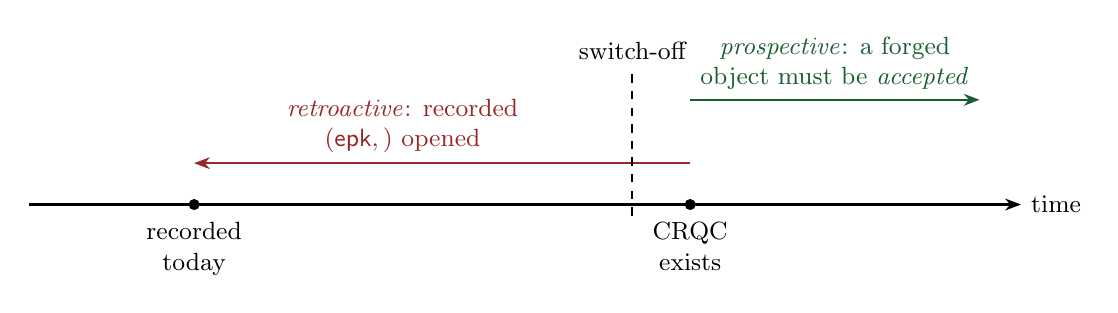
\begin{tikzpicture}[x=1.05cm, y=0.7cm, >={Stealth[length=2mm]},
  lab/.style={font=\small, align=center}]
\draw[->, thick] (0,0) -- (12,0) node[right, font=\small] {time};
\fill (2,0) circle (2pt);
\node[lab, below=3pt] at (2,0) {recorded\\today};
\fill (8,0) circle (2pt);
\node[lab, below=3pt] at (8,0) {CRQC\\exists};
\draw[<-, thick, arbred] (2,0.75) -- (8,0.75)
  node[pos=0.42, above, lab] {\emph{retroactive}: recorded\\
  $(\epk, \wbICenc)$ opened};
\draw[->, thick, arb] (8,1.9) -- (11.5,1.9)
  node[midway, above, lab] {\emph{prospective}: a forged\\object must
  be \emph{accepted}};
\draw[dashed, thick] (7.3,-0.2) -- (7.3,2.45) node[above, font=\small]
  {switch-off};
\end{tikzpicture}}
\end{center}
\Write
\begin{enumerate}
  \item ``CRQC = a quantum computer running Shor at scale: discrete logs
    in polynomial time; every group assumption falls.''
  \item Under the red arrow: ``exploitable the day the adversary exists''.
  \item Under the green arrow: ``a validator must \emph{accept} the
    forgery; switch off first''.
  \item Bottom line: ``Orchard, both pools: one retroactive break''.
\end{enumerate}
\Say
\textbf{Start from the adversary, not the calendar.} A CRQC runs Shor's
algorithm at scale and takes discrete logarithms in polynomial time.
Every group assumption in this workshop falls together, so asking
\emph{whether} is unproductive; the useful axis is reversibility.

\textbf{Retroactive breaks act on data already recorded.} The red arrow
runs backwards: what is on chain today is exploitable the day the
adversary exists, and no later consensus change can help. Prospective
breaks need a validator to \emph{accept} a forged object; switching the
mechanism off before that day removes acceptance. That is the dashed
line.

\textbf{Orchard, in both pools, has one retroactive break} --- the note
encryption, next board. Everything else on the integrity stack is
prospective.

\textbf{The contrast.} Bitcoin has no ciphertext to open, but a
silent-payment scan key has the same retroactive shape, and an exposed
public key is the prospective case.
\Avoid
Any date for the CRQC or for switch-off: the axis is an ordering, not a
calendar.
\src{\emph{Ironwood Guide}, ``The reversibility taxonomy and the
epistemic bins''; \emph{Crypto Guide}, ``The quantum caveat: Shor's
algorithm''}
\end{board}

\begin{board}{Retroactive: harvest now, decrypt later}{none --- privacy
  of the note}
\Write
\begin{enumerate}
  \item Published per Action: $(\epk, \wbICenc)$.
  \item The one discrete-log link: Diffie--Hellman between \esk{} and
    \pkd; ``KDF and AEAD above it are symmetric''.
  \item The attack, as one line:
    \[
    \ivk = \log_{\gd}\pkd
    \quad\Longrightarrow\quad
    K = \mathrm{KDF}\bigl([\ivk]\,\epk, \ldots\bigr)
    \]
  \item ``One logarithm per \ivk{} scope, then the recipient's own
    trial-decryption loop over the recorded chain.''
  \item Recovered per note: $(d, v, \mathsf{rseed}, \mathsf{memo})$ ---
    past and future.
  \item Example: Bob's $1.5$ ZEC and the memo.
\end{enumerate}
\Say
\textbf{Each Action publishes an ephemeral key and a ciphertext.} Their
confidentiality rests on exactly one discrete-log link, the
Diffie--Hellman between \esk{} and \pkd. The KDF and the AEAD above it
are symmetric and are not the weak layer.

\textbf{The attack is one logarithm and then honest work.} An adversary
holding a recipient's address computes $\ivk = \log_{\gd}\pkd$ once ---
one logarithm for the lifetime of that \ivk{} scope --- and then runs
the recipient's own trial-decryption loop over the recorded chain. For
every Action, $[\ivk]\,\epk$ feeds the KDF. Out comes every $(d, v,
\mathsf{rseed}, \mathsf{memo})$ ever sent to any diversified address
sharing that \ivk, past and future alike.

\textbf{Bring it back to the example.} Bob's address went to Alice.
Whoever else holds that address can one day read the $1.5$ ZEC and the
memo. Storage today, the logarithm later: harvest now, decrypt later.
\Avoid
``The solved \ivk{} yields \dk{} and \ovk'': those are derived from
\fvk, not from \ivk. Any claim that the KDF or the AEAD is the weak
layer.
\src{\emph{Ironwood Guide}, ``The retroactive break: harvest now, decrypt
later''}
\end{board}

\begin{board}{Retroactive: two limits, and the bin}{none --- privacy of
  the note}
\Write
\begin{enumerate}
  \item Limit 1: ``\ivk{} views, never spends; \asksym{} not exposed''.
  \item Limit 2: ``keyed by the address: no $(d, \pkd)$, no base \gd,
    no target \pkd''.
  \item Bin: \emph{open problem} --- ``nothing deployed or specified
    protects even future ciphertexts (ZIP-2005 non-requirement);
    recorded ones unrepairable''.
  \item Bitcoin column: silent payments --- one logarithm of the scan
    key replays the scan; amount and memo never hidden.
\end{enumerate}
\Say
\textbf{Two limits bound the damage.} First, \ivk{} is a viewing
capability: no spend authority is conferred, and \asksym{} is not
exposed --- its exposure is the prospective case. Second, the attack is
keyed by the address. Without $(d, \pkd)$ the adversary has neither the
base \gd{} nor the target \pkd, and no known efficient generic route
recovers the plaintext from the ciphertext alone.

\textbf{The bin is open problem.} Nothing deployed and nothing specified
protects even future ciphertexts; ZIP-2005 excludes privacy by an
explicit non-requirement. The recorded ciphertexts are unrepairable by
construction: any upgrade alters only ciphertexts not yet created.

\textbf{The contrast.} Bitcoin has no ciphertext to open, but silent
payments carry the same shape: one logarithm of the published scan key
replays the recipient's scan over recorded history and links everything
that address ever received. There is no analogue for the amount and the
memo, because Bitcoin never hid them.
\Avoid
``ZIP-2005 fixes this'': it repairs binding, not privacy. Deriving
$(\dk, \ovk)$ from \ivk.
\src{\emph{Ironwood Guide}, ``The retroactive break: harvest now, decrypt
later''; ZIP-2005, ``Non-requirements''}
\end{board}

\begin{board}{Prospective: the discrete-log integrity stack}{all four}
\Draw
Two columns, ``construction'' and ``with the generators' logarithms
known''; write the rows in this order:
\begin{enumerate}
  \item Sinsemilla binding (\NoteCommit, \CommitIvk): a second note under
    an on-chain \cmx{} --- balance breaks silently, turnstile-bounded; a
    second $(\aksym, \nksym)$ for the same \ivk{} --- a spendability
    forgery.
  \item Value commitment, binding signature: any \cvsym{} reopens to any
    value; a solved $\mathsf{bvk}$ forges the signature --- inflation,
    turnstile-bounded.
  \item Spend authorisation (RedPallas): one logarithm of \aksym{} or of
    any published \rksym{} forges spend authority; theft still needs a
    witness or a proof forgery.
  \item Proof soundness (IPA on Vesta): commitment equivocation; the
    knowledge-soundness reduction no longer holds.
\end{enumerate}
\Write
Under the table: ``recorded \cvsym{} perfectly hiding; $\alpha$ masks
\rksym; transcripts simulatable; without the address, no generic route
to these secrets''.
\Say
\textbf{Shor invalidates the reductions; it does not turn them into
attacks by itself.} Each construction gets its own concrete
consequence, so take the four rows one at a time.

\textbf{Sinsemilla loses binding first.} With the generators'
logarithms known, a second note opens under an on-chain \cmx: balance
breaks silently, bounded only by the turnstile. A second $(\aksym,
\nksym)$ pair for the same \ivk{} is a spendability forgery.

\textbf{Value commitments and the binding signature follow.} Any
\cvsym{} reopens to any value, and a solved $\mathsf{bvk}$ forges the
binding signature: inflation, again turnstile-bounded. For spend
authorisation, one logarithm of \aksym{} or of any published \rksym{}
forges authority --- but theft still needs a witness or a proof forgery.
For proof soundness, the IPA commitment can be equivocated and the
knowledge-soundness reduction no longer holds.

\textbf{What the recorded fields still do not give away.} Recorded
\cvsym{} values stay perfectly hiding, $\alpha$ masks \rksym, and
transcripts are simulatable. Without the address, no generic route
pulls these secrets from the recorded fields.
\Avoid
``Turnstile-bounded means detected'': a counterfeit inside a pool is
undetectable; the turnstile caps what can leave. ``The pool is
auditable.''
\src{\emph{Ironwood Guide}, ``Prospective breaks: the discrete-log
integrity stack''}
\end{board}

\begin{board}{Why the integrity breaks are prospective}{all four}
\Write
\begin{enumerate}
  \item ``A forged object --- proof, signature, commitment opening ---
    must be \emph{accepted}, at current height under current rules.''
  \item ``Switch off before the CRQC $\Rightarrow$ no acceptance; history
    anchored by chain work and upgrade policy.''
  \item Residue 1: switch-off must precede the \emph{first} forgery.
  \item Residue 2: honest funds inside a disabled pool need a way out
    $\Rightarrow$ ZIP-2005.
\end{enumerate}
\Say
\textbf{Every integrity attack has to be accepted by a validator.} A
forged proof, signature or commitment opening is worthless until a node
takes it, and acceptance happens at current height under current rules.
That is what makes the four rows prospective.

\textbf{So switching off first works.} Disabling the discrete-log pools
before a CRQC exists removes acceptance of new transactions under those
rules; settled history stays anchored by chain work and upgrade policy.

\textbf{Two residues.} The switch-off must precede the \emph{first}
forgery --- an attack landed inside the window is not repaired
afterwards. And honest funds inside a disabled pool need another way
out. That second residue is the problem ZIP-2005 exists to solve.

\textbf{The contrast.} Bitcoin has the same shape: ECDSA and Schnorr
fall to one logarithm of an exposed public key, and the forged spend
must still be mined.
\Avoid
A schedule for the switch-off: none is specified.
\src{\emph{Ironwood Guide}, ``Prospective breaks: the discrete-log
integrity stack''; \emph{Crypto Guide}, ``The quantum caveat: Shor's
algorithm''}
\end{board}

% compute/i_limits.py:
%   grover: 2^256 classical preimage evaluations -> ~2^128 quantum
%   bht collision: 2^(n/3) = 2^85 queries (needs ~2^92 bits of QRAM; not
%     the slide's number)
\begin{board}{The symmetric backbone survives}{authorised}
\Write
\begin{enumerate}
  \item BLAKE2b: $\mathsf{PRFexpand}$ (every key and note-randomness
    derivation), KDF, outgoing cipher key, RedPallas challenge, ZIP-244
    digests; ZIP-32 Orchard tree hardened-only.
  \item Poseidon: the nullifier PRF, keyed by \nksym{} --- a heuristic,
    classically and quantumly alike.
  \item Grover:
    \[
    2^{256} \text{ classical evaluations} \;\longrightarrow\;
    \approx 2^{128} \text{ quantum ones}
    \]
  \item ``Best implementable generic collision attack: still the
    classical parallel one.''
  \item Bottom line: ``ownership stays \emph{provable} after it stops
    being \emph{enforceable}''.
\end{enumerate}
\Say
\textbf{Two primitive families carry no discrete-log structure.}
BLAKE2b serves $\mathsf{PRFexpand}$, hence every key and
note-randomness derivation, the KDF, the outgoing cipher key, the
RedPallas challenge and the ZIP-244 digests; the ZIP-32 Orchard tree is
hardened-only and built entirely from it. Poseidon serves the nullifier
PRF keyed by \nksym{}, a cryptanalytic heuristic classically and
quantumly alike.

\textbf{Only generic speedups apply.} Grover halves preimage security:
$2^{256}$ classical evaluations become about $2^{128}$ quantum ones.
The best implementable generic collision attack remains the classical
parallel one.

\textbf{The load-bearing consequence.} A seed holder can still prove,
by re-executing the hardened derivations, that their keys descend from
their seed. Ownership stays provable after the assumption that made it
enforceable has fallen. That is the fact ZIP-2005 builds on.

\textbf{The contrast.} SHA-256 and hardened BIP-32 derivation stand on
the same ground.
\src{\emph{Ironwood Guide}, ``Primitives facing only generic speedups'';
\emph{Crypto Guide}, ``The quantum caveat: Shor's algorithm''}
\end{board}

% compute/b_quantum.py:
%   log2 N = log2 p_Vesta = 254.0000
%   q = 2^60: log2(q^3/N) = -74.0; log2(q^2/N) = -134.0
%   pre_rcm = 1+32+32+8+32+32 = 137 bytes
\begin{board}{ZIP-2005: the hashed trapdoor}{exists}
\Write
\begin{enumerate}
  \item The Ironwood derivation, written out in full:
    \[
    \rcm := \mathrm{ToScalar}\bigl(\mathsf{PRFexpand}_{\mathsf{rseed}}(
    \mathtt{0x0B} \,\|\, \gd^\star \,\|\, \pkd^\star \,\|\,
    \mathrm{LE}_{64}(v) \,\|\, \mathrm{LE}_{256}(\rho) \,\|\,
    \mathrm{LE}_{256}(\psi))\bigr)
    \]
  \item Under it: ``$137$-byte preimage --- every note field traverses
    BLAKE2b into the trapdoor''.
  \item ``Under a CRQC, \NoteCommit{} alone is not binding.''
  \item ``$\mathsf{PRFexpand}$ as a random oracle: two honest notes on
    one commitment = a collision event; bound $O(q^3/N)$, about
    $2^{-74}$ at $q = 2^{60}$.''
  \item ``Post-quantum binding \emph{provided a verifier checks the
    derivation} --- no deployed clause does.''
  \item Legacy $\mathtt{0x02}$ notes: $\mathtt{0x05} \,\|\, \rho$ only
    $\Rightarrow$ unrecoverable $\Rightarrow$ the seal.
\end{enumerate}
\Say
\textbf{Recall the one note-level difference between the pools.} An
Ironwood note derives its trapdoor \rcm{} by hashing every note field:
a $137$-byte preimage through BLAKE2b, tagged $\mathtt{0x0B}$.

\textbf{Why that matters under a CRQC.} The commitment \NoteCommit{}
alone is not binding once Sinsemilla's collision resistance falls, and
it is the first thing to fall. Model $\mathsf{PRFexpand}$ as a random oracle:
opening one commitment to two honestly derived notes becomes a
collision-type event with no group structure for Shor to exploit. The
bound is $O(q^3/N)$ in the QROM, about $2^{-74}$ at $q = 2^{60}$
queries.

\textbf{The binding is conditional.} The composite is post-quantum
binding \emph{provided a verifier checks the derivation}. No deployed
clause does --- the circuit checks the commitment, not the derivation
behind its trapdoor. That check is the Recovery Statement's job.

\textbf{Legacy notes hash only $\mathtt{0x05} \,\|\, \rho$.} They are
unrecoverable, and that is why the Orchard pool is sealed.

\textbf{The contrast.} Bitcoin ownership is a public key exposed at
spend. The hardened derivation behind it is symmetric too, but no rule
reads it; the exposed key alone decides a spend.
\Avoid
Treating $\rho$ in the preimage as a tree position: it is the per-note
uniqueness seed. ``ZIP-2005 makes Orchard quantum-secure.''
\src{\emph{Ironwood Guide}, ``The note seed: Ironwood derivations (lead
byte $\mathtt{0x03}$)''; ``ZIP-2005: quantum recoverability''; ``The
seal: three rules''}
\end{board}

% compute/b_quantum.py:
%   Recovery Statement cost: 7 BLAKE2b-512 compressions, 1 BLAKE3
%     compression, 2 Sinsemilla commitments, 2 Pallas scalar
%     multiplications, 1 Merkle path
\begin{board}{Recoverability, not resistance}{exists; authorised}
\Write
\begin{enumerate}
  \item Heading: ``Recovery Statement --- proved one day, post-quantum
    proof system, re-hashed tree''.
  \item The chain of claims, top to bottom: key derivations from
    $\mathsf{sk}$; $\ivk = \CommitIvk$; $\pkd = [\ivk]\,\gd$; $\psi$ and
    \rcm{} derivations; the commitment; a membership path; the
    nullifier; the $\alpha$ re-randomisation.
  \item Cost: $7$ BLAKE2b-512 compressions, $1$ BLAKE3 compression, $2$
    Sinsemilla commitments, $2$ Pallas scalar multiplications, a Merkle
    path.
  \item Box: ``binding only; privacy unchanged; opens no ciphertext''.
\end{enumerate}
\Say
\textbf{The Recovery Statement is what a holder would one day prove.}
In a post-quantum proof system, over a re-hashed tree, the holder shows
the whole chain: the key derivations from $\mathsf{sk}$, $\ivk =
\CommitIvk$, $\pkd = [\ivk]\,\gd$, the $\psi$ and \rcm{} derivations,
the commitment, a membership path, the nullifier, and the $\alpha$
re-randomisation.

\textbf{The cost is mostly hashing.} Seven BLAKE2b-512 compressions,
one BLAKE3 compression, two Sinsemilla commitments, two Pallas scalar
multiplications and a Merkle path.

\textbf{Binding only, privacy unchanged.} The statement proves, with no
group assumption, that one seed derives a committed note, its nullifier
and its \rksym. It opens no ciphertext; the harvested corpus is
untouched by it.
\Avoid
``Quantum resistance'': the strategy is recoverability. The statement
does not exist as a deployed proof; it is what would be proved.
\src{\emph{Ironwood Guide}, ``ZIP-2005: quantum recoverability'';
``Strategy: recoverability, not resistance''}
\end{board}

\begin{board}{ZIP-2005: deployed, specified, designed, open}
  {exists; authorised}
\Draw
Four rows, one bin each, written top to bottom:
\begin{enumerate}
  \item \emph{specified and deployed}: the $\mathtt{0x03}$ derivation and
    the three seal rules --- every Ironwood output is recoverable.
  \item \emph{specified, undeployed}: the quantum-key path
    ($\mathsf{qsk}$, $\mathsf{qk}$); no consensus rule.
  \item \emph{designed, unspecified}: the Recovery Protocol --- proof
    system, collapsing tree hash, linking commitments all unfixed.
  \item \emph{open}: post-quantum proofs and signatures for ongoing
    spends; the switch-off schedule.
\end{enumerate}
\Write
Under the rows: ``Sprout, Sapling, Orchard-pool notes: unrecoverable
$\Rightarrow$ sweep into Ironwood, ongoing; change already routed
there''. Then: ``the harvested corpus accrues now''.
\Say
\textbf{Sort ZIP-2005 into the bins.} Specified and deployed: the
$\mathtt{0x03}$ derivation and the three seal rules, so every Ironwood
output is recoverable. Specified but undeployed: the quantum-key path,
$\mathsf{qsk}$ and $\mathsf{qk}$, with no consensus rule behind it.
Designed but unspecified: the Recovery Protocol --- proof system,
collapsing tree hash and linking commitments all unfixed. Open:
post-quantum proofs and signatures for ongoing spends, and the
switch-off schedule.

\textbf{The consequence is forced migration.} Sprout, Sapling and
Orchard-pool notes are unrecoverable, so ZIP-2005 tells wallets to sweep
everything into Ironwood as an ongoing process. Deployed today, change
is already routed there.

\textbf{The one cost the strategy cannot answer.} The harvested corpus
accrues now.
\Avoid
A horizon for the switch-off: the schedule is an open problem.
``Fully post-quantum'': binding is repaired, privacy is not.
\src{\emph{Ironwood Guide}, ``ZIP-2005: quantum recoverability'';
``Strategy: recoverability, not resistance''; ``Change and wallet
posture''}
\end{board}

\begin{board}{Beyond the core: what each one adds}{all four unchanged}
\Draw
Three columns --- name, what it adds, Bitcoin --- written row by row:
\begin{enumerate}
  \item FROST: $t$-of-$n$ custody of \asksym; the aggregate is an
    ordinary spend-auth signature under \rksym{} --- a Taproot FROST
    suite.
  \item FlyClient: logarithmic chain proofs, difficulty-weighted sampling
    over a Merkle mountain range --- SPV fetches every header.
  \item ZSA: issued assets, per-asset notes and value commitments,
    issuance, burn --- Elements' issued assets.
  \item Crosslink: proof of work kept, plus a trailing BFT finality layer
    cross-linked with it --- confirmations, never finality.
\end{enumerate}
\Write
Under the table: ``none of the four adds privacy: custody, chain
verification, assets, settlement --- hiding unchanged''.
\Say
\textbf{Four extensions, one row each.} FROST gives $t$-of-$n$ custody
of \asksym; the aggregate is an ordinary spend-auth signature under
\rksym, and the verifier is untouched. FlyClient gives logarithmic
chain proofs by difficulty-weighted sampling over a Merkle mountain
range. ZSA gives issued assets: per-asset notes
and value commitments, issuance and burn. Crosslink keeps proof of work
and adds a trailing BFT finality layer cross-linked with it.

\textbf{Each has a Bitcoin neighbour.} A Taproot FROST suite; SPV, which
fetches every header; Elements' issued assets; and confirmations, which
are never finality.

\textbf{The one thing to emphasise.} None of the four adds privacy. They
add custody, chain verification, assets and settlement to a core whose
hiding is unchanged.
\Avoid
A multiplicative re-randomisation in the FROST row: the aggregate sits
under the same additive \rksym.
\src{\emph{FROST Guide}, ``Scope''; \emph{FlyClient Guide}, ``The
deployment boundary, stated at the outset''; ``The cost of header-only
verification''; \emph{ZSA Guide}, ``Method: the three bins for ZSA'';
\emph{Crosslink Guide}, ``Scope, status, and sources''}
\end{board}

\begin{board}{Beyond the core: the bins}{all four unchanged}
\Draw
Two columns --- name, bin as the volume states it --- row by row:
\begin{enumerate}
  \item FROST: \emph{specified} --- RFC 9591 and ZIP-312 (Draft); shipped
    as a library; no consensus rule names it; key generation in no ZIP.
  \item FlyClient: commitment \emph{deployed and consensus-critical}
    (ZIP-221, its root committed in every header since Heartwood);
    proofs \emph{unbuilt} --- no server serves one, no client asks; the
    Zcash instantiation designed, not specified.
  \item ZSA: core \emph{specified} in Draft ZIPs 226 and 227; the carrier
    --- v6 wire format, digests, lead byte, fees --- \emph{unspecified}
    since the ZIPs that held it were withdrawn; outside ZIP-259's NU7
    scope.
  \item Crosslink: \emph{design stage} --- no ZIP, nothing activated on
    mainnet or testnet; a feature net runs prototype code; construction
    rules \emph{designed but unspecified}.
\end{enumerate}
\Write
Under the table, the three bins: \emph{specified} / \emph{designed but
unspecified} / \emph{open problem}; ``deployed behaviour cites the
implementation and the specification instead''.
\Say
\textbf{Same four rows, now sorted by what actually exists.} FROST is
specified --- RFC 9591 and ZIP-312, a Draft --- and shipped as a
library; no consensus rule names it, and key generation is in no ZIP.
FlyClient's commitment is deployed and consensus-critical: ZIP-221's
root sits in every header since Heartwood. Its proofs are unbuilt ---
no server serves one, no client asks --- and the Zcash instantiation is
designed, not specified.

\textbf{ZSA and Crosslink are further out.} The ZSA core is specified in
Draft ZIPs 226 and 227, but the carrier --- v6 wire format, digests,
lead byte, fees --- is unspecified since the ZIPs that held it were
withdrawn, and ZIP-259 does not include it in NU7. Crosslink is design stage: no
ZIP, nothing activated on mainnet or testnet, a feature net running
prototype code, construction rules designed but unspecified.

\textbf{The bins are the volumes' method.} Specified, designed but
unspecified, open problem --- and deployed behaviour cites the
implementation and the specification instead.
\Avoid
``FlyClient is deployed'': the commitment is, the proofs are unbuilt.
Any activation height.
\src{\emph{FROST Guide}, ``The three-bin rule''; \emph{FlyClient Guide},
``The deployment boundary, stated at the outset''; ``The light-client
stack consumes none of it''; \emph{ZSA Guide}, ``Status''; ``Method: the
three bins for ZSA''; \emph{Crosslink Guide}, ``The three bins, and a
proved tag''; ``Scope, status, and sources''}
\end{board}

\begin{board}{Where each one sits}{all four unchanged}
\Draw
\begin{enumerate}
  \item Four boxes stacked vertically, top to bottom: ``block header'',
    ``chain selection'', ``Action statement'', ``spend-auth signature''.
    Shade the third box.
  \item To the right of each box, a tag: FlyClient --- reads a root
    already committed; Crosslink --- a finality layer beside PoW; ZSA
    --- the only one inside the circuit; FROST --- the same signature,
    more signers.
\end{enumerate}
\begin{center}
\resizebox{0.6\textwidth}{!}{%
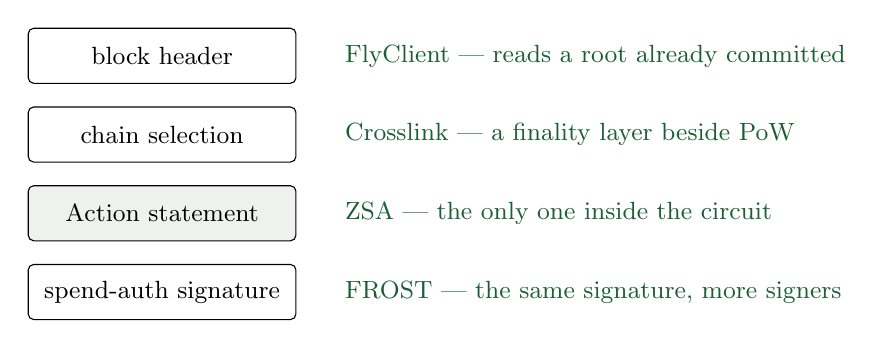
\begin{tikzpicture}[x=1cm, y=1cm, >={Stealth[length=2mm]},
  layer/.style={draw, rounded corners=2pt, minimum height=7mm,
    minimum width=34mm, font=\small, align=center},
  tag/.style={font=\small, text=arb, anchor=west}]
\node[layer] (hdr) at (0,3.0) {block header};
\node[layer] (cons) at (0,2.0) {chain selection};
\node[layer, fill=arb!8] (stmt) at (0,1.0) {Action statement};
\node[layer] (sig) at (0,0) {spend-auth signature};
\node[tag] at (2.2,3.0) {FlyClient --- reads a root already committed};
\node[tag] at (2.2,2.0) {Crosslink --- a finality layer beside PoW};
\node[tag] at (2.2,1.0) {ZSA --- the only one inside the circuit};
\node[tag] at (2.2,0) {FROST --- the same signature, more signers};
\end{tikzpicture}}
\end{center}
\Write
Beside the shaded box: ``ZSA only: Asset Base witnessed once; A1, A2 on
a per-asset commitment; A4 by variable-base multiplication; A3 dummy
skip kept for the native asset alone; split notes''. Under the stack:
``the other three leave the ten clauses as they are''.
\Say
\textbf{Place each extension on the stack you already know.} FlyClient
reads a root the header already commits. Crosslink adds a finality
layer beside proof of work, at the chain-selection layer. FROST
produces the same spend-auth signature with more signers. Only ZSA sits
inside the circuit.

\textbf{What ZSA changes in the statement.} An Asset Base witnessed
once; A1 and A2 on a per-asset commitment; A4 by variable-base
multiplication; the A3 dummy skip kept for the native asset alone; and
split notes.

\textbf{The one thing to emphasise.} The other three leave the ten
clauses exactly as they are.
\src{\emph{ZSA Guide}, ``The Action statement, extended''; \emph{FROST
Guide}, ``Scope''; \emph{FlyClient Guide}, ``The deployment boundary,
stated at the outset''; \emph{Crosslink Guide}, ``Scope, status, and
sources''}
\end{board}

% compute/a_checks.py:
%   (1) coin exists      Bitcoin: UTXO lookup          shielded: commitment
%       in an append-only tree + membership proof (A3)
%   (2) authorised       Bitcoin: script + signature   shielded: key
%       knowledge in the circuit (A6/A7) + re-randomised signature
%   (3) not spent twice  Bitcoin: UTXO deleted         shielded: nullifier,
%       published once, in the nullifier set (A5)
%   (4) conserved        Bitcoin: sum(in) >= sum(out)  shielded: homomorphic
%       value commitments (A4) + binding signature
\begin{board}{Takeaways: four checks, four mechanisms}{all four}
\Draw
Three columns --- check, Bitcoin, Zcash --- one row per check, in the
order of the spine:
\begin{enumerate}
  \item coin exists: UTXO lookup --- a commitment in an append-only tree;
    membership proven under an anchor, the position a private witness
    (A3).
  \item authorised: script and signature --- the circuit ties \rksym{} to
    \aksym{} (A6) and \aksym, \nksym{} to the note's address (A7); the
    node's signature check under \rksym{} proves $\rsk = \asksym +
    \alpha$.
  \item not spent twice: the UTXO is deleted --- the nullifier, keyed by
    \nksym{} and seeded by $\rho$: revealed once, rejected on repeat,
    unlinkable to \cmsym{} (A5).
  \item conserved: $\sum \mathrm{in} \ge \sum \mathrm{out}$ in the clear
    --- homomorphic value commitments (A4); the binding signature proves
    knowledge of $\sum \rcv$; fully shielded, valueBalance is the fee.
\end{enumerate}
\Write
Under the table: ``a stranger still performs all four; the note is never
seen''.
\Say
\textbf{Close on the spine.} Four checks a Bitcoin node makes by
looking at the coin; four mechanisms that let a stranger make the same
checks without ever seeing the note.

\textbf{Existence and authorisation.} The coin is a commitment in an
append-only tree, membership proven under an anchor with the position
a private witness. Authorisation is the circuit tying \rksym{} to
\aksym{} and \aksym, \nksym{} to the note's address, plus the node's
signature check under \rksym, which proves $\rsk = \asksym + \alpha$.

\textbf{Double spend and conservation.} The nullifier, keyed by
\nksym{} and seeded by $\rho$, is revealed once, rejected on repeat and
unlinkable to \cmsym. Conservation is homomorphic value commitments and
a binding signature proving knowledge of $\sum \rcv$; fully shielded,
valueBalance is the fee.

\textbf{The one sentence to leave on the board.} A stranger still
performs all four; the note is never seen.
\Avoid
A multiplicative form, $\rsk = \alpha \cdot \asksym$ or
$\rksym = [\alpha]\,\aksym$: the re-randomisation is additive.
Describing $\rho$ as the leaf position: the position is a private
witness of A3 and never enters the nullifier.
\src{\emph{Ironwood Guide}, ``The four requirements on a shielded
payment''; ``What a node verifies, without ever observing the note'';
``The Action statement, formally''}
\end{board}

\begin{board}{Where to read more: the Zcash Arboretum}{all four}
\Write
\begin{enumerate}
  \item Foundations: \emph{Math Guide} (fields, curves, hardness);
    \emph{Crypto Guide} (the toolbox's primitives); \emph{Halo 2 Guide}
    (the proof system, in full).
  \item Deployed protocol: \emph{Consensus Guide} (the consensus part);
    \emph{Ironwood Guide} (the spine of this workshop); \emph{Wallet
    Guide} (keys, fees, the pipeline, and what the server learns).
  \item Frontier: \emph{FlyClient}, \emph{ZSA}, \emph{Crosslink} and
    \emph{FROST Guides}, each with its bins visible.
  \item Bottom line: ``all non-normative --- the protocol specification
    and the ZIPs are authoritative''.
\end{enumerate}
\Say
\textbf{Three shelves.} Foundations for the mathematics, the primitives
and the proof system in full; deployed protocol for consensus, the
Ironwood spine of this workshop, wallets and the light-client server;
frontier for the four extensions, each with its bins visible.

\textbf{None of it is normative.} The protocol specification and the
ZIPs are authoritative, and every volume cites the section it draws on.
\end{board}

%% ---- 12-backup.tex
\section{Backup --- optional boards}

Every board in this section is optional: reach for one when a question
calls for it, and skip the section otherwise. No board here carries a
figure; three carry a table, given as rows in writing order.

\begin{board}{Sources --- the volumes, the specification, the
  ZIPs}{optional}
\Write
\begin{itemize}
  \item Volumes (non-normative): \emph{Ironwood} (the shielded critical
    path); \emph{Halo 2}, \emph{Wallet}, \emph{Crypto},
    \emph{Consensus}, \emph{Math}; one row each from \emph{FROST},
    \emph{FlyClient}, \emph{ZSA}, \emph{Crosslink}.
  \item Normative: the protocol specification; the ZIPs.
  \item Final or Active: 32 keys, 203 expiry, 209 pool balances,
    213 shielded coinbase, 221 history tree, 244 digests, 316 unified
    addresses, 317 fees.
  \item Draft: 229 v6 format (the two pools), 258 the Ironwood upgrade,
    307 compact blocks, 312 FROST, 315 wallet practice, 318 migration,
    326 wallets after the seal, 374 PCZT.
  \item Proposed: 2005 quantum recoverability. Reserved stub: 2006 the
    cross-address restriction.
  \item Bins: \emph{specified} / \emph{designed but unspecified} /
    \emph{open problem}.
\end{itemize}
\Say
\textbf{Everything in this workshop traces to a volume, and every deployed
claim to the specification or a ZIP.} The volumes are non-normative: the
Ironwood Guide carries the shielded critical path; the Halo 2, Wallet,
Crypto, Consensus and Math Guides carry the rest; the FROST,
FlyClient, ZSA and Crosslink Guides each supplied one row.

\textbf{Normative means the protocol specification and the ZIPs.} Read
the three ZIP lists off the board. One footnote on 318, migration: it was
a Reserved stub at the pinned zips checkout, \texttt{69610984}, and a
Draft at the recheck, \texttt{dd1667ff}.

\textbf{The rule for every slide you saw:} a deployed claim cites a
specification section or a ZIP; a design-stage claim carries its bin ---
specified, designed but unspecified, open problem.

\textbf{The Bitcoin contrast: BIPs, and no specification.} In Bitcoin the
reference client's behaviour is the definition. Here the specification is
a document, and a node implements it.
\Ask
What is normative here? The specification and the ZIPs; the volumes are
not.
\src{\emph{Ironwood Guide}, ``Two pools, one protocol: doors and the v6
transaction''; \emph{Consensus Guide}, ``Sources and their standing''}
\end{board}

\begin{board}{Implementation snapshots, as the volumes cite
  them}{optional}
\Draw
\begin{enumerate}
  \item Two columns, headed \emph{Volume} and \emph{Snapshot}.
  \item Ironwood: \textsf{orchard} 0.15.0 (the \textsf{librustzcash}
    pin); \textsf{orchard} \texttt{bef8a27} (circuit, cross-address);
    \textsf{librustzcash} \texttt{e30517e4}; \textsf{zips}
    \texttt{69610984}, rechecked at \texttt{dd1667ff}.
  \item Halo 2: \textsf{halo2\_proofs} 0.3.2; \textsf{halo2\_gadgets}
    0.5.0; \textsf{orchard} 0.15.3.
  \item Wallet: \textsf{librustzcash} \texttt{e30517e4}, later snapshot
    \texttt{91f448b5}; \textsf{zips} \texttt{c6b7035};
    synchronisation: \textsf{librustzcash} \texttt{e30517e4};
    \textsf{lightwalletd} \texttt{61fee32e}; \textsf{Zaino}
    \texttt{0e057e22}; \textsf{zips} \texttt{6961098}.
  \item Consensus: \textsf{zips} \texttt{69610984}; \textsf{zebra}
    \texttt{fa7657f1c}; \textsf{librustzcash} \texttt{e30517e43};
    rechecked at \textsf{zips} \texttt{e753a6a3}.
\end{enumerate}
\Write
Only the heading: \emph{snapshots, as the volumes cite them}. Write a row
when a question asks for it; otherwise read the rows out.
\Say
\textbf{Each volume pins the implementation it cites.} This board is the
answer to ``which version?'' for four of the volumes: the Ironwood
Guide's \textsf{orchard} and \textsf{librustzcash}
pins and its zips checkout with the recheck; the Halo 2 Guide's
\textsf{halo2\_proofs}, \textsf{halo2\_gadgets} and \textsf{orchard}
pins; the Wallet Guide's later \textsf{librustzcash} snapshot and its
\textsf{lightwalletd} and \textsf{Zaino} pins; the Consensus
Guide's \textsf{zebra} pin and its own zips recheck.

\textbf{A Bitcoin Core release number does the same job.} A claim about
a default is a claim about one version, and this table is where that
version lives.
\src{\emph{Ironwood Guide}, ``Two pools, one protocol: doors and the v6
transaction''; \emph{Halo 2 Guide}, ``From statement to circuit:
arithmetisation in practice''; \emph{Wallet Guide}, ``Diversified and
unified addresses (ZIP-316)''; ``Normative status and
wire-format history''; \emph{Consensus Guide}, ``Sources and their
standing''}
\end{board}

\begin{board}{Implementation snapshots, continued}{optional}
\Draw
\begin{enumerate}
  \item Same two columns, \emph{Volume} and \emph{Snapshot}.
  \item FROST: \textsf{frost} \texttt{0966bd1}; \textsf{reddsa}
    \texttt{63c6ac0}; \textsf{zips} \texttt{e753a6a3}.
  \item FlyClient: \textsf{zcash\_history} 0.5.0; \textsf{zips}
    \texttt{e753a6a3}.
  \item ZSA: \textsf{zips} \texttt{69610984}, rechecked at
    \texttt{e753a6a3}.
  \item Crosslink: tfl-book \texttt{fe6e1d6}; \textsf{zips}
    \texttt{e753a6a}.
  \item Crypto: no baseline pin; one design-stage cite, the
    \textsf{orchard} fork \texttt{cf801a5} (ZSA issuance).
  \item Math: no implementation pin; instances cite the specification.
\end{enumerate}
\Write
Only the heading: \emph{snapshots, continued}. Rows on request.
\Say
\textbf{The frontier volumes pin the same way.} FROST, FlyClient and
Crosslink each pin an artefact and a zips checkout; ZSA pins a zips
checkout and its recheck.

\textbf{Two volumes pin no deployed implementation.} The Crypto Guide
has no baseline pin --- one design-stage cite only, the \textsf{orchard}
fork for ZSA issuance. The Math Guide has no implementation pin at all:
its instances cite the specification.
\src{\emph{FROST Guide}, ``The source ladder''; \emph{FlyClient Guide},
``Sources and pinning''; \emph{ZSA Guide}, ``Sources''; \emph{Crosslink
Guide}, ``The source landscape''; \emph{Crypto Guide}, ``The transparent
layer's schemes: ECDSA and BIP-340 over secp256k1''}
\end{board}

\begin{board}{Scope}{optional}
\Write
\begin{itemize}
  \item A wallet default = the snapshot the volume cites, not every
    wallet.
  \item A node rail = Zebra, named only for the reorg window and the
    tie-break.
  \item Three toys: a prime-order group (balance); the $\F_{97}$ circuit
    (the proof system); the additive $\mathbb{Z}_{97}$ stand-in (the IPA
    fold, no discrete-log hardness). One mechanism each; no soundness
    estimated.
  \item Bins: \emph{specified} (a published artefact pins it down);
    \emph{designed but unspecified} (an informal source describes it);
    \emph{open problem} (no artefact exists).
  \item A deployed rule may still carry a Draft ZIP: bin and deployment
    tracked separately.
\end{itemize}
\Say
\textbf{Every default you heard today was one version's default.} A
wallet default describes the snapshot the volume cites, not every
wallet; a node rail describes Zebra, and Zebra was named only for the
reorg window and the tie-break. A Bitcoin Core release number does the
same job: a claim about a default is a claim about one version.

\textbf{The three toys isolated one mechanism each.} The prime-order
group stood in for balance, the $\F_{97}$ circuit for the proof system,
the additive $\mathbb{Z}_{97}$ group for the IPA fold --- that last one
with no discrete-log hardness at all. None of them estimates soundness.

\textbf{The bins are the volumes' bins.} Specified: a published artefact
pins it down. Designed but unspecified: an informal source describes it.
Open problem: no artefact exists.

\textbf{The Bitcoin contrast is a BIP's status field.} The difference is
that here a deployed rule may still carry a Draft ZIP, so the bin and
the deployment are tracked separately.
\Ask
Which toy had no discrete-log hardness? The additive $\mathbb{Z}_{97}$
stand-in for the IPA fold.
\src{\emph{Ironwood Guide}, ``Two pools, one protocol: doors and the v6
transaction''; \emph{Consensus Guide}, ``Sources and their standing''}
\end{board}

\begin{board}{The Pasta field discipline --- where each object
  lives}{optional}
\Draw
\begin{enumerate}
  \item Three columns, headed \emph{lives in}, \emph{elements},
    \emph{role}.
  \item \Fpv{} (Pallas \emph{scalar} field): $\asksym, \rivk, \rcm,
    \rcv, \alpha, \rsk, \esk, \mathsf{bsk}$ --- multiply points.
  \item \Fpp{} (Pallas \emph{base} field): $\nksym, \rho, \psi, \ivk,
    \cmx, \nfsym$ --- the circuit's native field.
  \item $\Ep(\Fpp)$ (Pallas points): $\aksym, \rksym, \gd, \pkd, \epk,
    \cmsym, \cvsym$ --- group elements.
  \item bit strings: $\mathsf{sk}, \mathsf{rseed}, \dk, \ovk$ ($256$);
    $d$ ($88$) --- keys, seeds, the diversifier.
\end{enumerate}
\Write
\begin{itemize}
  \item One rule: multiplies a point $\Rightarrow$ scalar modulo the
    group order $p_{\Vesta}$; hashed or compared by the circuit
    $\Rightarrow$ base-field element; consumed by BLAKE2b $\Rightarrow$
    byte string.
  \item Two base-field elements act as scalars: $\pkd = [\ivk]\,\gd$
    and the nullifier's $F_{\nksym}(\rho) + \psi$ --- valid because
    $p_{\Pallas} < p_{\Vesta}$ (both $255$ bits).
  \item Bitcoin's secp256k1: coordinates modulo $p$, scalars modulo $n$;
    ECDSA $r := x(R) \bmod n$.
\end{itemize}
\Say
\textbf{One rule sorts every symbol of the workshop.} What multiplies a
point is a scalar modulo the group order $p_{\Vesta}$; what the circuit
hashes or compares is a base-field element; what BLAKE2b consumes is a
byte string. Fill the table row by row and the rule does the sorting.

\textbf{Two elements cross the line, and one inequality makes that
legal.} The incoming viewing key $\ivk$ is a base-field element yet
multiplies $\gd$; the nullifier's $F_{\nksym}(\rho) + \psi$ is base-field
arithmetic yet scales a point. Both are valid only because $p_{\Pallas}
< p_{\Vesta}$ --- every base-field element is below the group order ---
with both primes $255$ bits.

\textbf{Bitcoin makes the same move once.} Its secp256k1 has the same two
fields, coordinates modulo $p$ and scalars modulo $n$, and ECDSA sets $r
:= x(R) \bmod n$. Nobody notices, because nothing recomputes it inside a
proof.
\Ask
Why may $\ivk$, a base-field element, multiply a point? Because
$p_{\Pallas} < p_{\Vesta}$: every base-field element is a valid scalar.
\Avoid
Do not gloss $\rho$, in the base-field row, as the note's position in
the tree: on this board it is the input to the nullifier's
$F_{\nksym}(\rho) + \psi$, a per-note field element.
\src{\emph{Ironwood Guide}, ``From $\mathsf{sk}$ to the spend-side
secrets''; ``Viewing keys''; ``The note and its commitment''; ``The
nullifier, and the loop back to minting''; ``Spend authorisation:
RedPallas re-randomisation''; \emph{Crypto Guide}, ``The transparent
layer's schemes: ECDSA and BIP-340 over secp256k1''}
\end{board}

\begin{board}{The Pasta field discipline --- the two primes}{optional}
\Write
\begin{gather*}
p_{\Pallas} = 2^{254} + \mathtt{0x224698fc094cf91b992d30ed00000001},\\
p_{\Vesta}  = 2^{254} + \mathtt{0x224698fc0994a8dd8c46eb2100000001}
\end{gather*}
\begin{itemize}
  \item The cycle: $\#\Ep_{\Pallas}(\Fpp) = p_{\Vesta}$ and
    $\#\Ep_{\Vesta}(\Fpv) = p_{\Pallas}$, both prime, cofactor $1$.
  \item Both $p - 1$ carry exactly $2^{32}$; the Action circuit uses
    $2^{11}$ rows. Both primes $\equiv 1 \bmod 3$: an order-$3$
    endomorphism.
  \item Deployed: circuit over \Fpp{}; commitments on Vesta, scalar field
    \Fpp{}; one half of the cycle, no recursion.
  \item Bitcoin's secp256k1: two-adicity $1$ (base), $6$ (scalar);
    largest domain $2$ (or $64$) points.
\end{itemize}
\Say
\textbf{Write the two primes and point at the shared prefix.} Both are
$2^{254}$ plus a tail; the tails differ. The cycle is the fact that the
Pallas curve over the Pallas base field has exactly $p_{\Vesta}$ points,
and the Vesta curve over its base field exactly $p_{\Pallas}$ --- both
prime, cofactor $1$. Each curve's scalar field is the other's base
field.

\textbf{Two properties of $p - 1$ are what the proof system wanted.}
Both carry exactly $2^{32}$, so power-of-two evaluation domains go up to
$2^{32}$; the Action circuit uses $2^{11}$ rows. Both primes are $1 \bmod
3$, so an order-$3$ endomorphism speeds scalar multiplication.

\textbf{Deployed is one half of the cycle.} The circuit's native field is
\Fpp{}, so Pallas points are native to it; its commitments live on
Vesta, whose scalar field is that same \Fpp{}. Recursion is not
deployed; verification amortises by batching instead.

\textbf{The Bitcoin contrast is secp256k1's two-adicity.}
Its $p - 1$ has two-adicity $1$, its scalar field $6$: the largest
power-of-two domain has $2$ (or $64$) points --- no room for a
$2^{11}$-row circuit, and no need for one. Say that this last number is
our own computation, not a volume figure.
\Ask
Why not build the circuit over secp256k1? Its two-adicity is $1$ (scalar
field $6$): the largest power-of-two domain has $2$ (or $64$) points,
far short of $2^{11}$ rows.
\src{\emph{Math Guide}, ``Pallas and Vesta assembled''; ``Base fields,
scalar fields, and the Pasta cycle''; \emph{Halo 2 Guide}, ``A cycle of
curves for efficient native recursion''; \emph{Ironwood Guide}, ``Flags,
public inputs, and circuit parameters''; protocol specification, ``Pallas
and Vesta''}
\end{board}

\begin{board}{Sinsemilla --- the hash}{optional --- exists}
\Write
\begin{align*}
Q(D) &:= \GroupHash^{\G}(\texttt{z.cash:SinsemillaQ},\, D),\\
P[m] &:= \GroupHash^{\G}(\texttt{z.cash:SinsemillaS},\, \mathrm{LE}_{32}(m)),
  \qquad 0 \le m < 2^{10}
\end{align*}
\[
\mathsf{Sinsemilla}_D(M) := \mathsf{Acc}_\ell, \qquad
\mathsf{Acc}_0 := Q(D), \qquad
\mathsf{Acc}_{i+1} := (\mathsf{Acc}_i \dotplus P[m_{i+1}]) \dotplus
\mathsf{Acc}_i
\]
\begin{itemize}
  \item Chunk width $k = 10$; at most $c = 253$ chunks ($2530$ bits);
    zero-padded on the right to a multiple of $10$ bits.
  \item Table $1024$ points, shared by every domain; $Q(D)$ per domain:
    $1025$ generators, all $\GroupHash$ outputs.
  \item Per chunk: one lookup, two incomplete additions ($\dotplus$).
    A $510$-bit message: $51$ rounds.
\end{itemize}
\Say
\textbf{Write the two generator families first, then the accumulator.}
The per-domain point $Q(D)$ and the $1024$-entry table $P[m]$ are all
$\GroupHash$ outputs --- $1025$ nothing-up-my-sleeve generators. The
table is shared by every domain; only $Q(D)$ changes with the domain.

\textbf{The hash is a walk.} Start the accumulator at $Q(D)$; for each
$10$-bit chunk, add the chunk's table point to the accumulator, then add
the old accumulator to the result. The message is zero-padded on the
right to a multiple of $10$ bits, and there are at most $253$ chunks,
$2530$ bits.

\textbf{The cost model is the point.} Each chunk costs one table lookup
and two incomplete additions; a $510$-bit message costs $51$ rounds, not
$510$ bit operations. Inside the circuit the table is a lookup argument.

\textbf{The Bitcoin contrast is SHA-256's home ground.} SHA-256 is tuned
for a CPU's word operations; inside a circuit every one of its bits is a
constraint. Sinsemilla is tuned for the circuit that must recompute it
--- and would be a poor CPU hash.
\Ask
How many rounds does a $510$-bit message cost? Fifty-one: one lookup and
two incomplete additions per $10$-bit chunk.
\src{\emph{Ironwood Guide}, ``Sinsemilla: hash, commitment, and short
forms''; ``Why Sinsemilla: in-circuit cost''; protocol specification,
``Sinsemilla Hash Function''}
\end{board}

\begin{board}{Sinsemilla --- the commitment and its short
  forms}{optional --- exists}
\Write
\begin{gather*}
\mathsf{SinsemillaCommit}_r(D, M) := \mathsf{Sinsemilla}_{D\|\texttt{-M}}(M)
  + [r]\,H_D,\\
\mathsf{ShortCommit}_r(D, M) := \Extract\bigl(\mathsf{SinsemillaCommit}_r(D,
  M)\bigr), \\
\mathsf{ShortHash}_D(M) := \Extract\bigl(\mathsf{Sinsemilla}_D(M)\bigr),
\qquad
H_D := \GroupHash^{\G}(D \,\|\, \texttt{-r},\ \varepsilon)
\end{gather*}
\begin{itemize}
  \item Instances: $\NoteCommit$ --- this commitment in its own domain, a
    point; the chain stores $\cmx$, its $x$.
  \item Key commitment $\CommitIvk$ --- $\mathsf{ShortCommit}$ over
    $\mathrm{LE}_{255}(\Extract(\aksym)) \,\|\, \mathrm{LE}_{255}(\nksym)$,
    $510$ bits, $51$ rounds.
  \item Tree node hash --- $\mathsf{ShortHash}$ over $520$ bits, $52$
    rounds.
\end{itemize}
\Say
\textbf{The commitment is the hash plus one blinding term.} Hash the
message in the domain's \texttt{-M} sub-domain, then add $[r]\,H_D$,
where $H_D$ is a $\GroupHash$ point in the domain's own \texttt{-r}
sub-domain. The short forms take the $x$-coordinate.

\textbf{Hiding needs no assumption.} For uniform $r$ the term $[r]\,H_D$
is uniform on the group, so the commitment reveals nothing about $M$.

\textbf{Binding rests on the two bases being unrelated.} The point $H_D$
sits in its own sub-domain, unrelated to $Q$ and the table as far as
anyone knows --- Pedersen's split of message base from blinding base.

\textbf{Three instances carried the workshop.} The note commitment
$\NoteCommit$ is this commitment in its own domain: a point, of which
the chain stores $\cmx$. The key commitment $\CommitIvk$ is the short
commitment over $\Extract(\aksym)$ and $\nksym$, $510$ bits, $51$
rounds. The tree's node hash is the short hash over $520$ bits, $52$
rounds.

\textbf{The Bitcoin bridge comes next.} Confidential Transactions'
$[v]V + [r]R$ is the one-slot Pedersen ancestor of this shape.
\Ask
Which side of the commitment needs an assumption, hiding or binding?
Binding: hiding is unconditional for uniform $r$; binding needs $H_D$
unrelated to $Q$ and the table.
\src{\emph{Ironwood Guide}, ``Sinsemilla: hash, commitment, and short
forms''; ``The note and its commitment''; ``The tree, its hash, and its
anchors''; protocol specification, ``Sinsemilla commitments''}
\end{board}

\begin{board}{Sinsemilla beside Confidential Transactions}{optional ---
  exists}
\Write
\[
\text{CT: } [v]\,V + [r]\,R; \quad
\text{Pedersen hash: } \textstyle\sum_{j} [m_j]\,P_j; \quad
\text{Sinsemilla: } [2^{\ell}]\,Q(D) + \textstyle\sum_{i}
  \bigl[2^{\ell - i}\bigr]\, P[m_i].
\]
\begin{itemize}
  \item One chunk: $[2]\,Q(D) + P[m_1]$ --- a lookup, not $[m_1]\,V$.
  \item Pedersen's coefficient has become Sinsemilla's index.
\end{itemize}
\Say
\textbf{Write the three forms on one line and read them left to right.}
Confidential Transactions' $[v]V + [r]R$ is the one-slot Pedersen
commitment. The Pedersen \emph{hash} extends it to a message with one
independent generator per chunk --- a table that grows with the message
length.

\textbf{Sinsemilla keeps the reduction and swaps the roles.} The
discrete-log collision reduction stays. But a chunk value now
\emph{selects} a point from one shared $1024$-entry table, and the
chunk's position supplies a fixed power-of-two weight. One table serves
every domain and every length up to $253$ chunks.

\textbf{The one-chunk case shows the swap.} A one-chunk Sinsemilla is
$[2]\,Q(D) + P[m_1]$: a lookup, not $[m_1]\,V$. Pedersen's coefficient
has become Sinsemilla's index.

\textbf{The Bitcoin contrast is what checks the opening.} In Elements the
opening of $[v]V + [r]R$ is range-proved by a Bulletproof; here
$\NoteCommit$'s opening is recomputed inside the Action proof, which is
what the lookup table is tuned for.
\Ask
What is a one-chunk Sinsemilla? The point $[2]\,Q(D) + P[m_1]$ --- the
chunk indexes the table instead of scaling a generator.
\src{\emph{Crypto Guide}, ``Sinsemilla: an algebraic hash-based
commitment''; \emph{Ironwood Guide}, ``Sinsemilla collision
resistance''; ``Why Sinsemilla: in-circuit cost''}
\end{board}

\begin{board}{Sinsemilla --- why a collision is a discrete
  logarithm}{optional --- exists}
\Write
\begin{gather*}
\mathsf{Sinsemilla}_D(M) = [2^{\ell}]\, Q(D) + \sum_{i=1}^{\ell}
  \bigl[2^{\ell - i}\bigr]\, P[m_i],
\qquad
\chi_j(m) := \sum_{i=1}^{\ell} 2^{\ell - i}\,[m_i = j],\\
\mathsf{Sinsemilla}_D(M) = \mathsf{Sinsemilla}_D(M') \ \Longrightarrow\
\sum_{j=0}^{2^{10}-1} \bigl[\chi_j(m) - \chi_j(m')\bigr]\, P[j] = \mathcal{O}.
\end{gather*}
\begin{itemize}
  \item Take $M \ne M'$ of equal length; $\chi_j$ taken modulo
    $p_{\Vesta}$.
  \item The bound $\ell \le 253$ keeps $2^{253} < p_{\Vesta}$: nothing
    wraps; $\chi(m)$ is injective.
\end{itemize}
\Say
\textbf{Unfold the accumulator, assuming no addition exception.} Every
chunk lands on a table generator with a power-of-two weight, and $Q(D)$
carries $2^{\ell}$. A repeated chunk value collects its weights into
$\chi_j$, taken modulo $p_{\Vesta}$. Take two distinct messages of equal
length.

\textbf{A collision is a relation among the generators.} Subtract the
two unfolded sums: the $Q$ terms cancel, and what remains is a linear
relation among the $P[j]$ with coefficients $\chi_j(m) - \chi_j(m')$.

\textbf{The relation is non-trivial because $\chi$ is injective.} The
binary digits of $\chi_j$ mark exactly where chunk value $j$ occurs, and
$\ell \le 253$ keeps $2^{253} < p_{\Vesta}$, so nothing wraps modulo the
group order. Distinct messages give distinct vectors, so some
coefficient is non-zero --- and a non-trivial relation among
independently sampled random-oracle generators is found only by
discrete logarithms.

\textbf{The Bitcoin contrast is the kind of assumption.} A SHA-256
collision would falsify a heuristic; a Sinsemilla collision would
compute a discrete logarithm on Pallas --- the same kind of assumption
that guards every Bitcoin key, on a different curve.
\Ask
Why does $\ell \le 253$ matter to the proof? It keeps $2^{253} <
p_{\Vesta}$, so the weight vector $\chi(m)$ never wraps and stays
injective.
\src{\emph{Ironwood Guide}, ``Sinsemilla collision resistance'';
\emph{Crypto Guide}, ``Sinsemilla: an algebraic hash-based commitment''}
\end{board}

\begin{board}{Sinsemilla --- the collision argument's fine
  print}{optional --- exists}
\Write
\[
\mathsf{Sinsemilla}_D(M) = -\mathsf{Sinsemilla}_D(M') \ \Longrightarrow\
[2^{\ell + 1}]\, Q(D) + \sum_{j}
  \bigl[\chi_j(m) + \chi_j(m')\bigr]\, P[j] = \mathcal{O}
\]
\begin{itemize}
  \item The coefficient $2^{\ell + 1} \ne 0 \bmod p_{\Vesta}$:
    non-trivial whether or not any chunk differs.
  \item Blinded forms: subtracting two openings adds $[r - r']\,H_D$ (or
    $[r + r']\,H_D$).
  \item Fixed length is load-bearing: every deployed use fixes its input
    length.
\end{itemize}
\Say
\textbf{Taking $x$-coordinates adds a second case.} The short forms
identify $P$ with $-P$, so a short-form collision is either the $+$ case
from the previous board or this $-$ case. Its $Q$-coefficient is
$2^{\ell + 1}$, non-zero modulo $p_{\Vesta}$, so the relation is
non-trivial whether or not any chunk differs.

\textbf{Blinding does not weaken it.} Subtracting two openings of the
commitment adds $[r - r']\,H_D$, or $[r + r']\,H_D$ in the $-$ case; the
message coefficients or the $Q$-coefficient keep the relation
non-trivial. Two distinct notes cannot share $\cmsym$, nor $\cmx$.

\textbf{The addition exception is not a loophole.} An undefined
incomplete addition is an equality between accumulator points --- itself
a relation among the same generators.

\textbf{Fixed length is load-bearing.} Zero-padding makes two messages of
different bit-lengths collide with no relation at all, so every deployed
use fixes its input length.

\textbf{The Bitcoin contrast is one hash at every length.} A Bitcoin hash
is used at every length; here each domain hashes one fixed length, and
the theorem is stated for exactly that.
\Ask
What breaks if the input length is not fixed? Zero-padding lets two
messages of different bit-lengths collide with no relation among the
generators at all.
\src{\emph{Ironwood Guide}, ``Sinsemilla collision resistance''}
\end{board}

\begin{board}{The seal --- three rules, in full}{optional --- conserved}
\Write
\begin{enumerate}
  \item \textbf{No issuance.} Coinbase: \emph{empty} Orchard component.
  \item \textbf{No circulation.} Every Orchard-pool Action:
    $\mathsf{enableCrossAddress} = 0$ --- enforced by the Action-circuit
    verifying key, selected by branch.
  \item \textbf{No entry.} Per transaction:
    $v_{\mathrm{balance}}^{\mathsf{Orchard}} \ge 0$.
\end{enumerate}
All three bind every transaction \emph{regardless of its version}
(ZIP-258).
\Say
\textbf{Three consensus rules seal the Orchard pool to spend-only.}
Number them as you write them. No issuance: a coinbase transaction
carries an empty Orchard component. No circulation: every Orchard-pool
Action has $\mathsf{enableCrossAddress} = 0$. No entry: per transaction,
$v_{\mathrm{balance}}^{\mathsf{Orchard}} \ge 0$ --- net value may leave
the pool, never enter.

\textbf{All three bind regardless of transaction version.} The second is
enforced by the Action-circuit verifying key, which consensus selects by
branch, so a v5 transaction cannot bypass it; ZIP-229 states the
version-independence explicitly.

\textbf{The second rule is the deepest, because it lives in the
circuit.} An Orchard-pool spend can pay only its own receiver. The
motive is recoverability: lead-byte-$\mathtt{0x02}$ notes cannot be
recovered after a quantum break, so consensus stops their circulation
and funnels the value out, while owners keep spending.

\textbf{Bitcoin retires no output type.} An early P2PK coin is spendable
today on the terms it was created with. Zcash retires a pool by sealing
its doors and metering its exit.
\Ask
Which of the three rules lives in the circuit? No circulation: the
verifying key, selected by branch, enforces $\mathsf{enableCrossAddress}
= 0$.
\Avoid
Do not say the seal applies only to v6 transactions: all three rules
bind every transaction regardless of its version.
\src{\emph{Ironwood Guide}, ``The seal: three rules''}
\end{board}

\begin{board}{The cross-address restriction, A10, in full}{optional ---
  conserved}
\Write
With $\delta := \mathsf{disableCrossAddress}$ and $x(\cdot), y(\cdot)$
the affine coordinates of a Pallas point:
\begin{gather*}
\delta \cdot \bigl(x(\gd_{\mathrm{old}}) - x(\gd_{\mathrm{new}})\bigr) = 0,
\qquad
\delta \cdot \bigl(y(\gd_{\mathrm{old}}) - y(\gd_{\mathrm{new}})\bigr) = 0,\\
\delta \cdot \bigl(x(\pkd_{\mathrm{old}}) - x(\pkd_{\mathrm{new}})\bigr) = 0,
\qquad
\delta \cdot \bigl(y(\pkd_{\mathrm{old}}) - y(\pkd_{\mathrm{new}})\bigr) = 0.
\end{gather*}
\begin{itemize}
  \item Public inputs, in order: $\mathsf{anchor}$; $\cvsym$ ($x$, $y$);
    $\nfsym$; $\rksym$ ($x$, $y$); $\cmx$; $\mathsf{enableSpends}$;
    $\mathsf{enableOutputs}$; $\delta$ (index $9$) --- ten in all.
  \item Same gate shape as A3: $v_{\mathrm{old}} \cdot (\mathsf{root} -
    \mathsf{anchor}) = 0$.
  \item Flags byte: $\mathtt{0b001}$ spends, $\mathtt{0b010}$ outputs,
    $\mathtt{0b100}$ cross-address; canonical $\mathtt{0b011}$ Orchard
    pool, $\mathtt{0b111}$ Ironwood.
\end{itemize}
\Say
\textbf{A10 is four equalities in the base field.} With $\delta$ the
disable flag, each equality says: if $\delta \ne 0$, one coordinate of
the old receiver equals the same coordinate of the new one. Four rows
cover $x$ and $y$ of $\gd$ and of $\pkd$, so with $\delta \ne 0$ the
receivers are equal as full points, not merely in $x$.

\textbf{The flag is the tenth public input.} Write the instance in order:
anchor, the two coordinates of $\cvsym$, $\nfsym$, the two of $\rksym$,
$\cmx$, $\mathsf{enableSpends}$, $\mathsf{enableOutputs}$, and $\delta$
at index $9$. The gate shape is A3's $v_{\mathrm{old}} \cdot
(\mathsf{root} - \mathsf{anchor}) = 0$ on four more rows.

\textbf{On the wire the polarity is reversed.} Bit $2$ of the flags byte
is $\mathsf{enableCrossAddress}$ --- bits $\mathtt{0b001}$ spends,
$\mathtt{0b010}$ outputs, $\mathtt{0b100}$ cross-address --- and the
canonical bytes are $\mathtt{0b011}$ for the Orchard pool and
$\mathtt{0b111}$ for Ironwood. Bit $2 = 0$ is what a v5 signer treating
it as reserved-zero already produces, so hardware signers keep signing
Orchard-pool unshielding unchanged.

\textbf{The Bitcoin contrast is how a rule narrows.} A soft fork narrows
which scripts are valid; here the narrowing is a new verifying key
selected by branch, and the wire change is one formerly reserved bit.
\Ask
Why four equalities and not two? Equality in $x$ alone would identify
$P$ with $-P$; $x$ and $y$ of both $\gd$ and $\pkd$ make the receivers
equal as full points.
\Avoid
Do not read $\delta$ as the wire flag: the wire carries
$\mathsf{enableCrossAddress}$, the instance carries its negation
$\mathsf{disableCrossAddress}$.
\src{\emph{Ironwood Guide}, ``The cross-address restriction (A10)'';
``Flags, public inputs, and circuit parameters''}
\end{board}

\begin{board}{Spending under the restriction}{optional --- conserved}
\Write
\[
(\mathsf{addr}_{\mathrm{old}},\ v_{\mathrm{old}}) \ \longrightarrow\
(\mathsf{addr}_{\mathrm{new}} = \mathsf{addr}_{\mathrm{old}},\
 v_{\mathrm{new}} = 0), \qquad
v_{\mathrm{balance}}^{\mathsf{Orchard}} = v_{\mathrm{old}} > 0.
\]
\begin{itemize}
  \item Pay anyone by \emph{exiting}: value leaves through a positive
    $v_{\mathrm{balance}}^{\mathsf{Orchard}}$; the output slot holds a
    fabricated zero-valued note to the spent note's own receiver.
  \item Self-sends stay possible; wallets forbid sends to
    \emph{external} Orchard-pool receivers (ZIP-326).
\end{itemize}
\Say
\textbf{An Action spends one note and creates one, and the restriction
fixes the created note's receiver.} Under A10 the created note must pay
the spent note's own receiver. So an owner pays anyone by exiting: the
real value leaves through a positive
$v_{\mathrm{balance}}^{\mathsf{Orchard}}$, and the output slot holds a
fabricated zero-valued note to the spent note's own receiver --- which
is also what keeps the Orchard tree growing.

\textbf{Self-sends survive by construction.} Paying an Orchard-pool
receiver requires a spend at that receiver, hence its spending key.
Wallet rules close the gap by forbidding sends to external Orchard-pool
receivers --- that is ZIP-326.

\textbf{The nearest Bitcoin concept is a covenant.} A covenant
restricting where an output may go is something Bitcoin script does not
offer; here it is one gate in a fixed circuit.
\Ask
How does an Orchard-pool owner pay Bob? By exiting: the value leaves as
a positive $v_{\mathrm{balance}}^{\mathsf{Orchard}}$, and the Action's
output is a zero-valued note to the spent note's own receiver.
\Avoid
Do not attribute the fabricated zero-valued output to the two-Action
minimum: it is there because every Action creates one note and the
restriction fixes that note's receiver.
\src{\emph{Ironwood Guide}, ``Spending under the restriction''}
\end{board}

\begin{board}{The fabricated output, and the restriction's
  standing}{optional}
\Write
\begin{itemize}
  \item Fabricated output: $C_{\mathrm{enc}}$ = random bytes.
  \item Inside a PCZT: recipient, value, $\mathsf{rseed}$ explicit
    $\Rightarrow$ signer classifies it as a tolerable dummy.
  \item \emph{Specified}: the flag's encoding, its consensus rule, the
    verifying-key selection by branch (ZIP-229, ZIP-258).
  \item \emph{Designed but unspecified}: the semantics of ``equal
    receivers'', the flag-to-instance mapping, the dummy-spend
    treatment.
  \item ZIP-2006: a Reserved stub.
\end{itemize}
\Say
\textbf{The fabrication is thorough.} The fabricated output's
$C_{\mathrm{enc}}$ is random bytes. A real encryption would let any
$\ivk$ holder --- including a later quantum adversary who recovered
$\ivk$ from a published address --- decrypt it and link the Action's
nullifier to the address. That is ZIP-326's reasoning.

\textbf{Between construction and signing the pretence is dropped.}
Inside a PCZT the fabricated output carries its recipient, value and
$\mathsf{rseed}$ explicitly, so a signer can classify it as a tolerable
dummy rather than an opaque payment.

\textbf{Its standing is split.} The restriction is deployed and enforced
by consensus, yet its owning ZIP-2006 is a Reserved stub. Specified: the
flag's encoding, its consensus rule, the verifying-key selection by
branch, in ZIP-229 and ZIP-258. Designed but unspecified: the normative
semantics of ``equal receivers'', the flag-to-instance mapping, the
dummy-spend treatment.

\textbf{The Bitcoin contrast is what a signer can see.} A Bitcoin signer
sees every output in the clear; a shielded signer needs the format to
tell it which output is a dummy.
\Ask
Why is the fabricated $C_{\mathrm{enc}}$ random rather than a real
encryption of the zero note? A real encryption would let an $\ivk$
holder --- a future one included --- link the Action's nullifier to the
address.
\src{\emph{Ironwood Guide}, ``Spending under the restriction''}
\end{board}

\begin{board}{The turnstile and migration}{optional --- conserved}
\Write
\[
\mathsf{IronwoodPoolBalance} := -\sum_{\mathrm{tx}}
  v_{\mathrm{balance}}^{\mathsf{Ironwood}}(\mathrm{tx}) \;\ge\; 0,
\qquad
v_{\mathrm{balance}}^{\mathsf{Orchard}} \ge 0 \text{ per transaction.}
\]
\begin{itemize}
  \item Migrating transaction: Orchard-pool spends with
    $v_{\mathrm{balance}}^{\mathsf{Orchard}} > 0$ $\rightarrow$
    transparent funds (fees and transparent outputs paid here)
    $\rightarrow$ $v_{\mathrm{balance}}^{\mathsf{Ironwood}} < 0$. Both
    fields cleartext.
  \item Pool balances: zero before the upgrade, never negative, summing
    to at most $\mathsf{MAX\_MONEY}$ (ZIP-209).
  \item Consensus caps nothing migration-specific; ZIP-318 recommends
    migration outputs of at most $10\,000$ ZEC.
  \item Ironwood tree capacity $2^{32}$; history tree gains three
    Ironwood fields.
\end{itemize}
\Say
\textbf{The turnstile is the instrument that retired Sprout.} It is a
one-way, publicly metered gate, and its consensus content is exactly the
two rules on the board: the seal's third, and the Ironwood pool-balance
row under ZIP-209's rule --- zero before the upgrade, never negative,
all pool balances summing to at most $\mathsf{MAX\_MONEY}$.

\textbf{A migrating transaction has a fixed shape.} It spends
Orchard-pool notes with $v_{\mathrm{balance}}^{\mathsf{Orchard}} > 0$
into its transparent funds --- where fees and transparent outputs are
paid too --- and absorbs them with $v_{\mathrm{balance}}^{\mathsf{Ironwood}}
< 0$. Both fields are cleartext: the amount crossing is public in every
transaction.

\textbf{Consensus caps nothing migration-specific.} ZIP-318 --- a
Reserved stub at the pin, a Draft at the later recheck --- recommends
migration outputs of at most $10\,000$ ZEC. The Ironwood tree has its
twin's $2^{32}$ capacity; the history tree gains three Ironwood fields.

\textbf{The Bitcoin contrast is the ledger row itself.} Bitcoin keeps no
per-type ledger row because every amount is already public; the pool
balance is the shielded ledger's one public number per pool.
\Ask
Where does a migrating transaction pay its fee? From the transparent
funds it passes through between the Orchard exit and the Ironwood
entry.
\Avoid
Do not say the pool is auditable: the balance row is the one public
number per pool, and what it does is meter the exit. Do not present
$10\,000$ ZEC as a consensus cap: it is a ZIP-318 recommendation.
\src{\emph{Ironwood Guide}, ``The turnstile and migration''; ``Pool
balances: ZIP-209 and its Ironwood analogue''}
\end{board}

\begin{board}{The quantum footnote --- what Part I left out}{optional}
\Write
\begin{itemize}
  \item One external $\ivk$ opens neither the internal-scope $\ivk$ nor
    any scope whose address the adversary never learns.
  \item The $\rcm$ derivation's collision bound: classical $O(q^2/N)$
    $\rightarrow$ QROM $O(q^3/N)$ (Zhandry, compressed oracle). At $q =
    2^{60}$, $N \approx 2^{254}$: $2^{-134}$ classically, $2^{-74}$ in
    the QROM.
  \item Recovery Statement, key half: $\mathsf{BindKeys}$ ---
    $\asksym$, $\aksym$, $\nksym$ from $\mathsf{sk}$; plus $\rivk$ from
    $\mathsf{sk}$ by $\mathsf{PRFexpand}$, or from a quantum key
    $\mathsf{qk}$ = one BLAKE3 compression of $\mathsf{qsk}$;
    signatures of knowledge over the sighash.
\end{itemize}
\Say
\textbf{The retroactive break has an edge.} One external $\ivk$ does not
open the separate internal-scope $\ivk$, where change lands (Part D),
nor any scope whose address the adversary never learns. The attack is
keyed by the address, not by the ciphertext.

\textbf{The binding bound has a price.} The classical collision bound
$O(q^2/N)$ on the $\rcm$ derivation lifts, by Zhandry's compressed-oracle
technique, to $O(q^3/N)$ in the quantum random-oracle model. At $q =
2^{60}$ and $N \approx 2^{254}$ that is about $2^{-134}$ classically
against $2^{-74}$: the lift costs a factor $q$.

\textbf{The Recovery Statement's key half is $\mathsf{BindKeys}$ plus
the $\rivk$ branch.} The name $\mathsf{BindKeys}$ covers the derivations
of $\asksym$, $\aksym$, $\nksym$ from $\mathsf{sk}$. The $\rivk$ branch
derives $\rivk$ from $\mathsf{sk}$ by
$\mathsf{PRFexpand}$, or --- where no single $\mathsf{sk}$ serves,
FROST-generated or hardware-held keys --- from a quantum key
$\mathsf{qk}$, one BLAKE3 compression of a secret $\mathsf{qsk}$, with
signatures of knowledge over the sighash tying the claimed keys to the
spend.

\textbf{Bitcoin's exposure is of Part I's table's kind, with two
differences.} A forged signature under an exposed public key must be
accepted. But a forged RedPallas signature alone spends nothing here ---
theft also needs the note's witness or a proof forgery --- and
counterfeit, not theft, is what the pool's exit caps.
\Ask
Does a recovered external $\ivk$ reach the change? No: change lands
under the separate internal-scope $\ivk$, which the external one does
not open.
\Avoid
Do not say change is found through $\ovk$: on this board the change is
reached only through the internal-scope $\ivk$, which the external
$\ivk$ does not open. Do not turn the $2^{-74}$ into a timing claim: it
is a bound at one query budget, not a clock.
\src{\emph{Ironwood Guide}, ``The retroactive break: harvest now, decrypt
later''; ``ZIP-2005: quantum recoverability''; ``Prospective breaks: the
discrete-log integrity stack''}
\end{board}

\end{document}
